%=====================================================================
%  《N=2 超对称规范理论中的 S-对偶导引》中文译注本 —— 主文件
%  底本：arXiv:hep-th/9701069v1
%  编译：xelatex main.tex（两遍）
%=====================================================================
\documentclass[UTF8,11pt,fontset=fandol,a4paper]{ctexart}
%=====================================================================
%  《N=2 超对称规范理论中的 S-对偶导引》中文译注本 —— 导言区
%  底本：L. Alvarez-Gaumé, S. F. Hassan, arXiv:hep-th/9701069v1
%        (CERN-TH/96-371), Fortsch. Phys. 45 (1997) 159--236, 82 pp.
%  编译方式：xelatex main.tex（两遍，第二遍生成目录与交叉引用）
%
%  说明：
%  1) 本文档类为 ctexart（论文体例），章节编号与原文严格一致；
%  2) 公式环境沿用原文的 equation / eqnarray 结构，公式编号由 LaTeX
%     自动生成，与原文 (1.1)--(4.x) 逐一对应。原文的简写宏
%     \beq \eeq \bea \eea \bq \eq 已在整理底本时展开为
%     标准环境，以方便教授直接在源码上删改；
%  3) % [Tutor Note: ...] 为审校批注（LaTeX 注释，编译后不显示）；
%  4) 符号约定：原文全文采用 (+,-,-,-) 号差，本译本一律照录，
%     不逐式改写为 (-,+,+,+)（详见 front.tex 第 2 节“符号约定说明”）。
%=====================================================================
\usepackage[a4paper,left=2cm,right=2cm,top=2.4cm,bottom=2.4cm,
            headheight=14pt]{geometry}
\usepackage{amsmath}
\usepackage{amssymb}
\usepackage{amsthm}
\usepackage{mathtools}
\usepackage{bm}
\usepackage{graphicx}
\usepackage{xcolor}
\usepackage[most]{tcolorbox}
\usepackage{caption}
\usepackage{enumitem}
\usepackage{booktabs}
\usepackage{array}
\usepackage{multirow}
\usepackage{fancyhdr}
\usepackage[unicode,colorlinks=true,linkcolor=blue!45!black,
            citecolor=blue!45!black,urlcolor=blue!45!black]{hyperref}
\usepackage{bookmark}

%---------------------- 版式与字体 ----------------------
\allowdisplaybreaks[4]
\linespread{1.32}
\setlength{\emergencystretch}{3em}
\setlength{\parindent}{2em}
\setlist{itemsep=2pt,topsep=3pt,parsep=0pt}
\renewcommand{\figurename}{图}
\captionsetup{font=small,labelsep=quad,justification=centering,skip=5pt}
\ctexset{
  section={format=\Large\bfseries\heiti, beforeskip=18pt, afterskip=8pt},
  subsection={format=\large\bfseries, beforeskip=12pt, afterskip=5pt},
  subsubsection={format=\normalsize\bfseries, beforeskip=8pt, afterskip=3pt}
}

%---------------------- 页眉页脚 ----------------------
\pagestyle{fancy}
\fancyhf{}
\fancyhead[L]{\small $N=2$ 超对称规范理论中的 $S$-对偶导引}
\fancyhead[R]{\small\rightmark}
\fancyfoot[C]{\thepage}
\renewcommand{\headrulewidth}{0.4pt}
\fancypagestyle{plain}{\fancyhf{}\fancyfoot[C]{\thepage}%
  \renewcommand{\headrulewidth}{0pt}}
\renewcommand{\sectionmark}[1]{\markright{\thesection\quad #1}}

%---------------------- 本节重点（Key Takeaways） ----------------------
% 每个 \section 标题之后使用：
%   \begin{keypoints} \item ... \end{keypoints}
\newtcolorbox{keypoints}{
  enhanced, breakable,
  colback=blue!3!white, colframe=blue!55!black,
  boxrule=0.6pt, arc=2pt,
  left=8pt, right=8pt, top=4pt, bottom=4pt,
  title={本节重点（Key Takeaways）},
  fonttitle=\bfseries\small, fontupper=\small,
  coltitle=white, colbacktitle=blue!55!black
}

%---------------------- 常用记号（与原文一致，勿改） ----------------------
\newcommand{\rd}{\mathrm{d}}
\newcommand{\Tr}{\operatorname{Tr}}
\newcommand{\tr}{\operatorname{tr}}
\newcommand{\Imag}{\operatorname{Im}}
\newcommand{\Real}{\operatorname{Re}}


%---------------------- PDF 元数据 ----------------------
\hypersetup{
  pdftitle={N=2 超对称规范理论中的 S-对偶导引（中文译注本）},
  pdfauthor={L. Alvarez-Gaume, S. F. Hassan; 中文译注},
  pdfsubject={arXiv:hep-th/9701069v1, Fortschr. Phys. 45 (1997) 159-236},
  pdfkeywords={N=2 supersymmetry, Seiberg-Witten, S-duality, monopole, 中译本}
}


\begin{document}

%=====================================================================
%  封面、摘要、译本说明
%  本文件由 Lead 撰写；译者不要修改。
%=====================================================================
\thispagestyle{empty}
\begin{center}
\vspace*{1.2cm}

{\heiti\LARGE $N=2$ 超对称规范理论中的 $S$-对偶导引}\\[10pt]
{\heiti\Large ——Seiberg--Witten 工作的教学式综述}\\[4pt]

\vspace{1.0cm}
{\large L. Alvarez-Gaum\'e,\quad S. F. Hassan}\\[6pt]
{\normalsize Theoretical Physics Division, CERN, CH-1211 Geneva 23}\\[4pt]
{\normalsize CERN-TH/96-371\quad hep-th/9701069\quad December 1996}\\[4pt]
{\normalsize 原载于\ Fortschr.\ Phys.\ \textbf{45} (1997) 159--236}

\vspace{1.2cm}
{\large\bfseries 中文译注本}\\[6pt]
{\normalsize 底本：arXiv:hep-th/9701069v1（82 页，含插图 7 幅）}\\[2pt]
{\normalsize 译文与审校批注：2026 年 10 月}

\vspace{1.0cm}
\begin{minipage}{0.86\textwidth}
\small
\textbf{内容简介}\quad 本讲义系统讲授 $N=2$ 超对称规范理论的精确结果：前半部分回顾规范场论中的磁单极
（狄拉克单极、't Hooft--Polyakov 单极、Bogomol'nyi 界与 BPS 态）以及超对称规范理论的构造；
后半部分详述 Seiberg--Witten 对 $SU(2)$、$N=2$ 纯规范理论及含物质理论低能有效作用量的精确求解，
包括模空间、单值变换、对偶性与 Seiberg--Witten 曲线。译文完整保留原文全部编号公式、交叉引用与文献
编号，并在关键推导处附学术级审校批注。
\end{minipage}

\vfill
{\small 编译方式：\texttt{xelatex main.tex}（两遍）}
\end{center}
\newpage

%=====================================================================
\section*{摘要}
\addcontentsline{toc}{section}{摘要}
%=====================================================================
本讲义旨在对 Seiberg 与 Witten 关于 $S$-对偶以及含物质与不含物质的 $N=2$ 超对称规范理论精确结果的工作，
作一教学式的导引。前半部分回顾规范场论中的磁单极与超对称规范理论的构造；后半部分阐述 Seiberg--Witten 的工作。
\medskip

\noindent\textbf{关键词：}\ 超对称；$N=2$ 规范理论；磁单极；电磁对偶；Seiberg--Witten 解；模空间；单值变换

\newpage

%=====================================================================
\section*{译本说明}
\addcontentsline{toc}{section}{译本说明}
%=====================================================================

\subsection*{一、底本与页码对照}

本译本以 arXiv:hep-th/9701069v1（1997 年 1 月 14 日提交，82 页，LaTeX 源码含 7 幅 EPS 插图）为唯一底本，
同时参考期刊版 Fortschr.\ Phys.\ \textbf{45} (1997) 159--236。原文 PDF 的页码对应关系为
\begin{center}
\textbf{原文 PDF 页号 = 原文印刷页号 + 1},
\end{center}
即 PDF 第 1 页为标题页，正文自 PDF 第 2 页（印刷页 1）起。本译本全部审校批注中的“原文 PDF 第 $N$ 页”
均按此约定标注，便于对照电子底本逐页核查。

原文共四节：第 1 节为规范场论中的磁单极；第 2 节为超对称规范理论；第 3 节为 $N=2$ 纯规范理论的
Seiberg--Witten 分析；第 4 节为含物质的情形。另有致谢与参考文献。

\subsection*{二、翻译与公式保真原则}

\begin{enumerate}
  \item \textbf{语义级翻译，不取字面对译。}术语以中文学术界通行译法为准（规范场论、和乐、反常、超场、
        手征多重态、单值变换等），首次出现时在批注中给出英文原词。
  \item \textbf{公式逐字符保真。}本译本直接以作者原始的 LaTeX 源码为工作底本，所有显示公式、行内公式、
        上下标、希腊字母、指标位置、花体与大写、以及公式编号均与原文逐一对应；原文用
        \verb|\beq|、\verb|\bea| 等简写宏书写的环境在整理底本时展开为 \verb|equation|、\verb|eqnarray|
        标准环境，数学内容一字未改。
  \item \textbf{编号与交叉引用。}公式编号沿用 LaTeX 自动编号，与原文 (1.1)--(4.x) 完全一致；
        原文的 \verb|\label|/\verb|\ref| 交叉引用机制予以保留并正常编译，正文中的式号可直接跳转。
  \item \textbf{不增删物理内容。}遇长难句或作者跳步处，译文保留原意并另加批注说明，绝不以猜测补足原文
        未写的物理内容。原文笔误一律保留原文形式，并在批注中如实指出。
  \item \textbf{参考文献。}文献条目保留原文英文，编号 [1]--[40] 与原文一致，便于与原文及引文索引对照。
\end{enumerate}

\subsection*{三、审校批注体例}

译本在源码中以 LaTeX 注释形式插入批注，格式固定为
\begin{center}
\verb|% [Tutor Note: ...]|
\end{center}
编译后不显示，供教授直接阅读源码时查阅。批注分四类：
\begin{itemize}
  \item \textbf{易错预警}：涉及张量缩并、指标升降、符号约定、全导数/边界项、$\epsilon$ 张量约定处，
        提示核对的具体位置与陷阱；
  \item \textbf{含糊点拨}：原文以 “It is obvious / One can show / It is easy to see” 等语跳过证明之处，
        补出被省略的核心逻辑、所依据的定理与可查文献；
  \item \textbf{原文笔误}：如实指出印刷错误（含拼写、符号、公式），并给出正确形式；
  \item \textbf{术语说明}：非常见译名首次出现时给出英文原词与文献中的异名。
\end{itemize}
全部批注在文末“审校批注索引”与随附的 \texttt{审校批注汇总.md} 中有汇总，便于不读源码时检索。

\subsection*{四、符号约定说明（重要）}

原文\textbf{通篇采用号差} $(+,-,-,-)$（Minkowski 度规 $\eta_{\mu\nu}=\mathrm{diag}(1,-1,-1,-1)$，
$\varepsilon^{0123}=+1$），并在第 1.1 节开宗明义地声明了这一约定。教授要求所有符号采用 $(-,+,+,+)$。
此处必须说明本译本的处理方式与理由：

\begin{enumerate}
  \item 号差不是排版细节，而是\textbf{贯穿全文的物理约定}：$F_{0i}$ 与电场 $E^i$ 的符号关系、
        费米子动能项与质量项的相对符号、超代数 $\{Q,\bar Q\}$ 的右端、中心荷 $Z$ 与 BPS 界的符号、
        $\theta$ 项与瞬子作用量的符号、Seiberg--Witten 曲线与椭圆积分的分支约定，全部与号差绑定。
  \item 若把 $(+,-,-,-)$ 逐式局部改写为 $(-,+,+,+)$，必须同时作整体替换
        $\eta_{\mu\nu}\to-\eta_{\mu\nu}$、$\gamma^\mu\to i\gamma^\mu$（以保证
        $\{\gamma^\mu,\gamma^\nu\}=2\eta^{\mu\nu}$ 不变），并相应调整作用量整体符号与费米场相位；
        这会使\textbf{每一个公式}都偏离原文，且极易在张量缩并与 $\gamma$ 矩阵迹的计算中引入隐蔽错误，
        与“无损、可与原文逐式对读”的翻译目标直接冲突。
  \item 因此本译本\textbf{严格照录原文的} $(+,-,-,-)$ \textbf{约定，不对任何公式作号差改写}。
        这样教授手边的原文、文献 [31,32]（Seiberg--Witten 原文）与本译本三者可以逐式对照。
        若教授需要 $(-,+,+,+)$ 版本，建议在通读本译本后，按上述整体规则统一重写，而不要逐式局部替换；
        任何局部替换都会在超荷代数、BPS 界与模空间度规的符号上造成自相矛盾。
  \item 第 1.1 节（原文 PDF 第 3--5 页）集中列出了全部约定（度规、$\gamma$ 矩阵、$\sigma^{\mu\nu}$、
        $D_\mu$、场强、$\theta$ 项等），建议先读该节再进入正文。
\end{enumerate}

\subsection*{五、插图}

原文共 7 幅插图（Figure 1--7），均为作者提供的 EPS 矢量图。本译本将原始 EPS 逐一转换为 PDF 矢量图
（保留矢量可缩放性），插入正文对应位置，并为每幅图补写中文图注、标注其在原文 PDF 中的位置。
需要说明：\textbf{原文对这 7 幅图只标注了 “Figure $n$”，没有说明性图注}；因此中文图注中明确区分了
“原文标签”与“译者据图补写的说明”，不加引号者即为译者补注，以免与原文混淆。

\begin{center}
\small
\begin{tabular}{@{}cccc@{}}
\toprule
图号 & 原文 PDF 页 & 内容 & 文件 \\
\midrule
图 1 & 第 7 页  & 狄拉克弦与磁单极磁场 & \texttt{figures/fig1.pdf} \\
图 2 & 第 15 页 & $S^2$ 上闭曲线的同伦类 & \texttt{figures/fig2.pdf} \\
图 3 & 第 60 页 & $u$ 平面上的奇点与单值变换 & \texttt{figures/fig3.pdf} \\
图 4 & 第 61 页 & $x$ 空间：双叶黎曼面 & \texttt{figures/fig4.pdf} \\
图 5 & 第 61 页 & 由环面理解 $x$ 空间 & \texttt{figures/fig5.pdf} \\
图 6 & 第 77 页 & $\lambda$ 平面上的分支点与积分路径 & \texttt{figures/fig6.pdf} \\
图 7 & 第 77 页 & 路径 $\Gamma_2$ 的变形 & \texttt{figures/fig7.pdf} \\
\bottomrule
\end{tabular}
\end{center}

\subsection*{六、编译与文件清单}

本译本为单文件主控、分文件组织的 LaTeX 工程，用 XeLaTeX 编译两遍：
\begin{center}
\verb|xelatex main.tex| \quad（两遍，第二遍生成目录与交叉引用）
\end{center}
依赖宏包均为 TeX Live 标准配置（\texttt{ctex}、\texttt{amsmath}、\texttt{amssymb}、\texttt{graphicx}、
\texttt{tcolorbox}、\texttt{caption}、\texttt{enumitem}、\texttt{fancyhdr}、\texttt{hyperref} 等）。
文件组织见随附 \texttt{README.md}。

\subsection*{七、致谢}

原文致谢对象保留原文语义；译文本身的工作由中文译注组完成。原文致谢见正文末尾。

\newpage


\newpage
\tableofcontents
\markboth{}{}
\newpage

%---------------------- 正文（译者分片，按原文顺序） ----------------------
\markboth{引言}{}
% ===== 分片 A：引言 + §1 标题与导语 + §1.1–§1.4（原文 PDF 第 2–9 页）=====
\section*{引言}
\addcontentsline{toc}{section}{引言}

\begin{keypoints}
\begin{itemize}
  \item \textbf{物理图像：}本讲义围绕 Seiberg 与 Witten 关于 $N=2$ 超对称量子色动力学（SQCD）精确结果的工作展开，读懂它需要预先备齐磁单极与超对称两块背景。
  \item \textbf{数学工具：}狄拉克磁单极与电荷量子化 $\to$ 't Hooft–Polyakov 磁单极与 Bogomol'nyi 界 $\to$ $N=1,2$ 超对称拉格朗日量与中心荷 $\to$ 模空间上的单值变换、完全椭圆积分与对偶。
  \item \textbf{关键结论：}全文分四节：§1 规范场论中的磁单极；§2 超对称规范理论；§3 $N=2$ 纯规范理论的 Seiberg–Witten 分析；§4 含物质场的推广。更完整的文献指引见 \cite{Lerche}。
\end{itemize}
\end{keypoints}

本讲义是 1995 年在意大利的里雅斯特（Trieste）暑期学校所作一系列讲座的书面整理稿，其成文远晚于讲座本身。讲座的目的是对 Seiberg 与 Witten 关于量子色动力学的 $N=2$ 超对称扩充之精确结果的工作，给出一个基础性的介绍。我们希望把深入研究其工作所需的全部背景材料集中在一处。我们设想的读者是已经修过量子场论课程的研究生，除此以外并不期望读者具备更多的背景知识就能跟上这些讲座。我们已尽力使讲解循序渐进、便于教学。在某些小节中，我们大量借用了已有的综述：例如在超对称的处理上我们遵循 Bagger 与 Wess \cite{WB}，在磁单极理论中则采用了 Goddard 与 Olive \cite{GO} 以及 S. Coleman \cite{coleman1,coleman2} 的综述。这些文献对这些课题给出了出色的阐述，我们也没有非要改进其讲述的充分理由。同样显而易见的是，我们大量引用了 Seiberg 与 Witten 的原始论文 \cite{SW-I,SW2}，但我们力图提供必要的工具，使有兴趣的学生和/或研究者更容易读懂这些论文。近来还出版了若干水平更高的讲义，其中可以找到更多细节以及与弦论的联系（例如可参见 W. Lerche 的讲义 \cite{Lerche}）。我们还想说明，我们并未试图穷尽地引用该课题的全部文献；更完整的参考文献列表可在 \cite{Lerche} 中找到。本文的文献列表意在为进入弦论与场论中对偶性这一迅速增长的文献提供入门指引。对于因未能列入其工作而可能感到不快的作者，我们深表歉意。

% [Tutor Note: 见原文 PDF 第 2 页引言第一段。文中“Trieste Summer School”指 1995 年在意大利的里雅斯特（Trieste）举办的暑期学校系列讲座，本讲义即这些讲座的整理稿；原文称其为“very late written version”（很晚才写成的版本），故译作“成文远晚于讲座本身”。]

本讲义分为四节，每一节又进一步细分为若干小节。第 1 节介绍规范场论中的磁单极。我们先讨论狄拉克磁单极与电荷量子化的思想，然后描述具有自发对称性破缺的规范理论中的 't Hooft–Polyakov 磁单极。随后我们引入 Bogomol'nyi 界与 BPS 态的概念。在此之后，我们描述磁单极的拓扑分类，然后叙述电磁对偶的 Montonen–Olive 猜想。本节最后，我们说明当拉格朗日量中存在 $\theta$ 项时，磁单极的电荷会因其磁荷而发生平移。第 2 节介绍超对称规范理论。我们首先描述超对称代数，以及它不含中心荷与含中心荷的表示，并讨论它在超场语言下的局域实现。然后构造 $N=1$ 的拉格朗日量，最后构造同时含规范多重态与物质多重态（超多重态）的 $N=2$ 超对称拉格朗日量。在本节末尾，我们分别在纯规范理论与含物质的理论中计算 $N=2$ 中心荷，并确立它与 BPS 界的关系。在前两节建立基础之后，第 3 节描述对规范群为 $SU(2)$ 的 $N=2$ 纯规范理论所作的 Seiberg–Witten 分析。在前两个小节中，我们讨论模空间的参数化与 $R$ 对称性的破缺。接着说明如何利用该理论的手征 $U(1)$ 反常得到低能有效作用量的单圈形式。本节其余部分则致力于借助对偶性以及理论模空间上的奇点结构求出精确的低能有效作用量。我们用完全椭圆积分表示这一精确解。在第 4 节中，我们简要描述对含 $N_f$ 个物质场的 $N=2$ $SU(2)$ 规范理论所作的 Seiberg–Witten 分析。在讨论这类理论的一般特征之后，我们说明其（对偶）群不再单纯是 $SL(2,Z)$。然后描述这些理论模空间上的奇点结构，并勾勒求得精确解的步骤。第 4 节的目的只是让读者对含物质理论的分析有所体会；若要更深入的理解，有兴趣的读者可参阅 Seiberg 与 Witten 的原始工作。

% [Tutor Note: 见原文 PDF 第 3 页引言第二段。原文称含物质时“the duality group is no longer pure $SL(2,Z)$”，其中“pure”指对偶群不再是整个 $SL(2,Z)$，而是它的真子群（同余子群）；具体形式与物质场的味数 $N_f$ 有关，详见原文第 4.6 节（原文 PDF 第 75 页起）。]

\section{规范场论中的磁单极}

\begin{keypoints}
\begin{itemize}
  \item \textbf{物理图像：}磁单极在规范场论中作为孤立子（拓扑缺陷）出现；'t Hooft–Polyakov 磁单极是 $SO(3)$ 规范理论经希格斯机制自发破缺到 $U(1)$ 后的非微扰态。
  \item \textbf{数学工具：}狄拉克弦与电荷量子化条件（式(\ref{XII})、(\ref{DSZ})）；磁单极的拓扑分类（同伦群）；Bogomol'nyi 界与 BPS 饱和。
  \item \textbf{关键结论：}$SO(3)$ Georgi–Glashow 模型的微扰谱为有质量希格斯粒子 $H$、光子 $\gamma$ 与 $W^\pm$ 玻色子，其非微扰谱中还包含磁单极与双子。
  \item \textbf{本节路线：}§1.1 约定与预备知识；§1.2 电荷量子化的半经典推导；§1.3 狄拉克弦；§1.4 Georgi–Glashow 模型。§1.5 之后的单极解、Bogomol'nyi 界、Montonen–Olive 猜想与 $\theta$ 项效应见后续小节。
\end{itemize}
\end{keypoints}

本节我们先回顾狄拉克磁单极的性质与电荷量子化的思想。然后描述具有自发对称性破缺的非阿贝尔规范理论中出现的磁单极与双子，并讨论它们的一般性质。我们还引入 Bogomol'nyi 界与 BPS 态的概念。在最后两个小节中，我们描述电磁对偶的 Montonen–Olive 猜想，以及 Witten 关于拉格朗日量中 $\theta$ 项的存在如何改变磁单极与双子电荷的论证。关于本节大部分材料更详细的讨论，读者可参阅 Goddard 与 Olive 的综述文章 \cite{GO}，以及 Coleman 的讲义 \cite{coleman1,coleman2}。

\subsection{约定与预备知识}

我们先陈述约定：我们始终取 $c=1$，并且几乎总取 $\hbar=1$，除非需要区分经典效应与量子效应。处理指标升降时，我们使用号差为 $\{ +,-,-,-\}$ 的平直 Minkowski 度规 $\eta$。此外，我们选取使麦克斯韦方程组取如下形式的单位：
\begin{equation}
\begin{array}{l}
\vec{\nabla}\cdot\vec{E}=\rho\,,\qquad\vec{\nabla}\times\vec{B}-
\partial \vec{E}/\partial t =\vec{j}\,,\\
\vec{\nabla}\cdot\vec{B}=0\,,\qquad \vec{\nabla}\times\vec{E} +
\partial\vec{B}/\partial t = 0\,.
\label{I}
\end{array}
\end{equation}
在这些单位下，库仑定律中出现因子 $(4 \pi)^{-1}$：对于位于原点的静态点状电荷 $q$，有 $\rho = q 
\delta^{3}(\vec{r})$。将第一个麦克斯韦方程在半径为 $r$ 的球面上积分并利用球对称性，得到
$\int_{S^2} \vec{E} \cdot d \vec{s}=4\pi r^2 E(r)=q$。因此，如前面所说，
$\vec{E}=q\vec{r}/4\pi r^{3}$。由 $\vec{E}=-\vec{\nabla}\phi$ 定义的静电势 $\phi$ 为
$\phi = q / 4 \pi r$。

% [Tutor Note: 见原文 PDF 第 3 页式 (1)。此处采用的是 $c=\hbar=1$ 且库仑定律带因子 $(4\pi)^{-1}$ 的“有理化”单位制（Lorentz–Heaviside 型），故点电荷场强为 $\vec{E}=q\vec{r}/4\pi r^{3}$ 而非 $q\vec{r}/r^{3}$。后文的 $4\pi$、$e=q/\hbar$ 以及磁荷 $g$ 的归一化全都由它确定；若换用 SI 或高斯制，电荷量子化条件会整体差一个 $4\pi$，核对时请务必以此单位制为准。]

在相对论记法中，引入四维势 $A^{\mu}= \{\phi, \vec{A}\}$。电场与磁场定义为相应场强张量 $F_{\mu\nu}$ 的分量，具体如下：
\begin{eqnarray}
F_{\mu \nu} & = &\partial_{\mu}A_{\nu} - \partial_{\nu}A_{\mu}\,,
\nonumber \\
F_{0i} & = &\partial_{0}A_{i} - \partial_{i}A_{0} =
- \partial_{0}A^{i} - \partial_{i}A^{0} = E^{i}\,,\nonumber \\
F_{ij} & = & \partial_{i}A_{j} - \partial_{j}A_{i} =
- (\partial_{i}A^{j} - \partial^{j}A_{i}) =
-\epsilon_{ijk} B^{k}\,,
\label{III}
\end{eqnarray}
于是 $B^i=-\frac{1}{2}\epsilon^{ijk}F_{jk}=-\frac{1}{2}
\epsilon^{oi\mu\nu}F_{\mu\nu}$。对偶场强张量由下式给出
$$
\widetilde F^{\mu \nu} = \frac{1}{2} \varepsilon^{\mu \nu \alpha
\beta} F_{\alpha \beta}\,,
$$
其中 $\varepsilon^{0123}=+1$。用分量记法，我们有
\begin{equation}
F^{\mu \nu} =
\left(
\begin{array}{cccc}
0 & -E_{x} & -E_{y} & -E_{z}  \\
E_{x} & 0 & -B_{z} & B_{y} \\
E_{y} & B_{z} & 0 & -B_{x} \\
E_{z} & -B_{x} & B_{y} & 0
\end{array}
\right)\,,
\qquad
\widetilde F^{\mu \nu} =
\left(
\begin{array}{cccc}
0 & -B_{x} & -B_{y} & -B_{z} \\
B_{x} & 0 & E_{z} & -E_{y} \\
B_{y} & -E_{z} & 0 & E_{x} \\
B_{z} & E_{y} & -E_{x} & 0
\end{array}
\right)\,.
\label{IV}
\end{equation}

% [Tutor Note: 见原文 PDF 第 3 页式 (2) 与第 4 页式 (3)。在号差 $(+,-,-,-)$、$\varepsilon^{0123}=+1$ 下，$F_{0i}=E^i$ 但升指标得 $F^{0i}=-E^i$，同理 $\widetilde F^{0i}=-B^i$；式 (3) 的两个矩阵里 $E$、$B$ 的符号分布正是这一约定的结果，此处是最容易漏掉负号的地方，请逐项核对。]

用电四维流 $j^{\mu}=\{\rho,\vec{j}\}$ 表示，麦克斯韦方程组取紧凑形式
\begin{equation}
\partial_\nu F^{\mu\nu}=-j^\mu\,,\qquad\partial_\nu\,\widetilde
F^{\mu\nu}=0\,. \label{V}
\end{equation}
注意当 $j^\mu =0$ 时，上述方程在替换 $\vec{E} \rightarrow \vec{B}, \vec{B} \rightarrow
-\vec{E}$ 下不变。这称为电磁对偶变换。当存在电源时，该变换不再是麦克斯韦方程组的对称性。为了使这些方程在 $j^{\mu}$ 非零时恢复对偶不变性，Dirac \cite{Dirac} 引入了磁四维流 $k^{\mu}=\{\sigma ,\vec{k}\}$，并把麦克斯韦方程组修改为
\begin{equation}
\partial_\nu F^{\mu\nu}=-j^\mu\,,\qquad\partial_\nu\,
\widetilde F^{\mu\nu}= -k^\mu \,.   
\label{VI}
\end{equation}
现在上述方程在场与流的联合对偶变换下不变，该变换可写为
\begin{equation}
F\rightarrow \widetilde F\,,\,\widetilde F\rightarrow-F\,;\qquad 
j^\mu\rightarrow k^\mu\,,\, k^\mu\rightarrow -j^\mu\,.
\label{emduality}
\end{equation}
注意方程组(\ref{VI})的完全不变群比这个离散对偶变换更大。事实上，它们在一个连续的 $SO(2)$ 群下不变，该群把电学量与磁学量相互旋转。

% [Tutor Note: 见原文 PDF 第 4 页式 (5)、(6)。要点有二：其一，对偶不变性只在场与流“同时”按式 (6) 变换时才成立，单独变换场并不是麦克斯韦方程组的对称性；其二，原文所说连续的 $SO(2)$ 群指 $(F,\widetilde F)$ 平面内的转动（等价于对复组合 $F+i\widetilde F$ 作相位变换），这正是后文 $S$ 对偶连续版本的雏形。]

对于点状电源与点状磁源，流密度可写为
\begin{eqnarray}
j^{\mu}(x) & = & \sum_{a} q_{a} \, \int \, dx_{a}^{\mu}
\delta^{4} (x - x_{a})\,, \nonumber \\
k^{\mu}(x) & = & \sum_{a} g_{a} \, \int \, dx_{a}^{\mu}
\delta^{4} (x - x_{a})\,.\nonumber
\end{eqnarray}
带有电荷 $q$ 与磁荷 $g$ 的粒子受到如下洛伦兹力：
$$
m\,\frac{d^2x^\mu}{d\tau^2}=(q F^{\mu\nu}+g\, \widetilde F^{\mu\nu})
\frac{dx_\nu}{d\tau}\,.
$$

尽管在运动方程的层面上，Dirac 对麦克斯韦理论的修改似乎无关紧要，但它在量子理论中有着极为非平凡的后果。认识这一问题的一个途径是注意到，在理论的量子表述中矢量势 $\vec{A}$ 是不可或缺的；另一方面，方程
$\vec{B}=\vec{\nabla}\times \vec{A}$ 与 $\vec{\nabla}\cdot\vec{B}\ne
0$ 并不相容，除非矢量势 $\vec{A}$ 带有奇点，因而并非整体良定义。结果表明，这些奇点依赖于规范选择，因此它们的存在不应当在实验上可观测。在可以仅用 $\vec B$ 表述的经典理论中，这一要求平凡地得到满足。然而在量子理论中，它导致了电荷量子化这一重要现象。下面我们先给出这一效应的半经典推导，然后描述基于狄拉克弦概念的推导。
 
\subsection{电荷量子化的半经典推导}

考虑一个非相对论性电荷 $q$，位于原点处强度为 $g$ 的磁单极附近。电荷 $q$ 受到力 $m\ddot{\vec{r}}=q\dot{\vec{r}}\times\vec{B}$，其中 $\vec{B}$ 是由 $\vec{B}= 
g\vec{r}/4\pi r^3$ 给出的磁单极场。在该力作用下，电荷的轨道角动量的变化由下式给出
$$
\frac{d}{dt}\left(\,m\vec{r}\times\dot{\vec{r}}\right) =
m\vec{r}\times\ddot{\vec{r}}= \frac{qg}{4 \pi r^{3}}\,
\vec{r}\times\left(\dot{\vec{r}}\times\vec{r}\right)= 
\frac{d}{dt}\left(\frac{qg}{4\pi}\,\frac{\vec{r}}{r}\right)\,.
$$
因此，系统的总守恒角动量为
\begin{equation}
\vec{J}=\vec{r}\times m\dot{\vec{r}}-\frac{qg}{4\pi}\,
\frac{\vec{r}}{r}\,.
\label{XI}
\end{equation}
右端第二项（以下记作 $\vec{J}_{em}$）是来自电磁场的贡献。这一项可以直接计算：电磁场的动量密度由其坡印廷矢量 $\vec{E}\times\vec{B}$ 给出，因此它对角动量的贡献为
$$
\vec{J}_{em} = \int \, d^{3}x \, \vec{r} \times
(\vec{E} \times \vec{B}) = \frac{g}{4 \pi} \,
\int \, d^{3} x \, \vec{r} \times
\left( \vec{E} \times \frac{\vec{r}}{r^{3}} \right)\,.
$$
写成分量，
\begin{eqnarray}
J^i_{em} & = & \frac{g}{4 \pi} \, \int \, d^{3}x E^{j}
\left( \delta_{ij} - \frac{x_i x_j}{r^{2}} \right )
\frac{1}{r} = \frac{g}{4 \pi} \, \int \, d^{3}x E^{j}
\partial_{j} (\hat{x}^{i}) \nonumber \\
& = & \frac{g}{4 \pi} \int_{S^2} \hat{x}^i \vec{E}\cdot \vec{ds} 
- \frac{g}{4 \pi} \, \int \, d^{3}x \vec{\nabla} \cdot
\vec{E} \hat{x}^{i}\,. 
\label{XIV}
\end{eqnarray}
当电、磁荷之间的距离与它们到边界 $S^2$ 的距离相比可以忽略时，第一个积分对 $\vec{J}_{em}$ 的贡献因球对称性而消失。于是只剩下
\begin{equation}
\vec{J}_{em}= -\frac{gq}{4 \pi} \hat{r}
\label{Jem}\,.
\end{equation}

% [Tutor Note: 见原文 PDF 第 5 页式 (8)。第二个等号是分部积分：$\partial_j\hat{x}^i=(\delta_{ij}-x_ix_j/r^2)/r$，再把 $E^j\partial_j\hat{x}^i$ 写成 $\partial_j(E^j\hat{x}^i)-\hat{x}^i\partial_j E^j$。原文只说“球对称使第一个积分消失”，对真正给出式 (9) 的 $\vec{\nabla}\cdot\vec{E}=q\delta^{3}(\vec{r})$ 一项轻轻带过——恰恰是原点处的 $\delta$ 源贡献了 $-qg/4\pi\,\hat{r}$。这是本段最容易“差一个符号”的地方，请按 $\partial_j\hat{x}^i$ 的符号重新核对。]

回到式(\ref{XI})，若假设轨道角动量是量子化的，则由此可得
\begin{equation}
\frac{qg}{4 \pi} = \frac{1}{2} n \hbar\,,
\label{XII}
\end{equation}
其中 $n$ 为整数。注意在上面的推导中，我们假设了电荷–磁单极系统的总角动量以半整数倍为单位量子化。考虑到我们并不需要把带电粒子或磁单极当作费米子，这是一个奇怪的假设：两个组分都是玻色子。然而结果表明情形确实如此，而且这种情形并不违反自旋–统计定理
\cite{Goldhaber,Wilczek}。我们不再进一步讨论这一问题，但要指出，下一小节给出的同一方程的推导并不依赖于这一假设。

% [Tutor Note: 见原文 PDF 第 6 页式 (10) 前一句。原文“if we assume that orbital angular momentum is quantized. Then it follows that”在句号处应作逗号（原文标点笔误），译文的句式已按正确逻辑重写。物理上这里假设的是“总角动量（含场角动量 $\vec{J}_{em}$）以 $n\hbar/2$ 量子化”，而非纯轨道角动量；随后原文承认这与两个组元都是玻色子相矛盾，并把解释归于文献 [5,6]（Goldhaber、Wilczek）。下一小节由狄拉克弦给出的推导不依赖此假设。]

式(\ref{XII})就是狄拉克电荷量子化条件。它意味着：如果宇宙中某处存在一个磁荷为 $g$ 的磁单极，那么所有电荷都以 $2\pi\hbar/g$ 为单位量子化。如果我们有若干纯电荷 $q_i$ 和若干纯磁荷 $g_j$，那么它们中任意一对都满足一个量子化条件：
\begin{equation}
\frac{q_{i}g_{j}}{4 \pi \hbar} = \frac{1}{2} n_{ij}
\label{XIII}
\end{equation}
因此，任何电荷都是 $2\pi\hbar/g_j$ 的整数倍。对给定的 $g_j$，设这些电荷的最大公因子为 $n_{0j}$。那么所有电荷都是 $q_{0}=n_{0j}2\pi\hbar /g_{j}$ 的倍数。注意 $q_0$ 本身未必存在于谱中。类似的考虑也适用于磁荷的量子化。

到目前为止，我们只处理了或者带电荷、或者带磁荷的粒子。现在我们考虑双子，即同时携带电荷与磁荷的粒子。考虑两个双子，其荷分别为 $(q_1,g_1)$ 与 $(q_2,g_2)$。对该系统，我们可以按(\ref{XIV})中的步骤重复 $\vec{J}_{em}$ 的计算，只是现在电磁场要分解为 $\vec{E}=\vec{E}_1+\vec{E}_2$ 与 $\vec{B}=\vec{B}_1+ \vec{B}_2$。容易求得结果为

\begin{equation}
\vec{J}_{em}=-\frac{1}{4\pi}\left(q_1 g_2 - q_2 g_1\right)\hat{r} 
\label{Jemd}
\end{equation}
于是电荷量子化条件推广为
\begin{equation}
\frac{q_1 g_2 - q_2 g_1}{4\pi\hbar}=\frac{1}{2} n_{12}
\label{DSZ}
\end{equation}
这称为 Dirac–Schwinger–Zwanziger 条件
\cite{Schwinger,Zwanziger}。该条件在 $SO(2)$ 变换 $(q+ig)\rightarrow e^{i\phi}(q+ig)$ 下不变，而后者也是(\ref{VI})的一个对称性。

% [Tutor Note: 见原文 PDF 第 6 页式 (13)。注意 $n_{12}$ 依赖两粒子的编号顺序，交换 $1\leftrightarrow2$ 时 $n_{12}\to-n_{12}$；而 $q_1g_2-q_2g_1$ 正是二维矢量 $(q_i,g_i)$ 的行列式，在 $(q_i,g_i)$ 整体 $SO(2)$ 转动下不变。这一“量子化条件与连续对偶相容”的事实，正是后文（§4）把对偶群视为 $SL(2,Z)$ 的子群、并研究其单值变换的出发点。]

\subsection{狄拉克弦}

下面我们给出狄拉克量子化条件的更严格推导，它基于狄拉克弦这一概念。用 $\vec{B}_{mon}$ 表示磁单极周围的磁场。由于 $\vec{\nabla}\cdot\vec{B}_{mon}\ne 0$，不可能构造一个良定义的 $\vec{A}_{mon}$ 使得
$\vec{B}_{mon}=\vec{\nabla} \vec{A}_{mon}$。为克服这一困难，Dirac 引入了一根半无限长的螺线管（或弦），它从 $(0,0,-\infty)$ 延伸到磁单极所在的位置 $(0,0,0)$。该螺线管携带磁场 $\vec{B}_{sol}=g\theta (-z)\delta(x)
\delta(y)\hat{z}$，它同样不是无散的。然而，总磁场
\begin{equation}
\vec{B}=\vec{B}_{mon}+\vec{B}_{sol}=\frac{g}{4\pi r^{2}}+g\theta(-z)
\delta(x)\delta(y)\hat{z}\,,
\end{equation}
满足 $\vec{\nabla}\cdot\vec{B}=g\delta(\vec{r})-g\delta(\vec{r}) 
=0$。因此，可以为磁单极–螺线管系统构造一个非奇异的 $\vec{A}=
\vec{A}_{mon}+\vec{A}_{sol}$。事实上，与狄拉克弦相联系的奇异 $\vec{A}_{sol}$ 正是用来抵消 $\vec{A}_{mon}$ 中的奇性的。$\vec{A}_{mon}$ 中奇点的位置、从而狄拉克弦的位置，可以通过奇异规范变换移动。既然狄拉克弦是人为构造的，它就应当是不可观测的，也不应对任何物理过程有贡献。然而，在 Aharonov–Bohm 实验中，弦的存在会通过对其相位的贡献影响电荷的波函数。沿一条环绕该弦、并围出面积 $S$ 的回路 $\Gamma$，由此得到的 Aharonov–Bohm 相位容易算出为
$$
e \oint_{\Gamma} \vec{A}_{sol} \cdot d \vec{l} = e \int_S
\vec{B}_{sol} \cdot d\vec{s} = e g\,.
$$
这里，$e=q/\hbar$ 是电磁耦合常数。只要
$$
e g = 2\pi n\,,
$$
该相位、从而狄拉克弦便是不可观测的，这再次给出狄拉克电荷量子化条件。

% [Tutor Note: 见原文 PDF 第 7 页第 2 行。原文写 $\vec{B}_{mon}=\vec{\nabla} \vec{A}_{mon}$，漏掉叉乘号，应为 $\vec{B}_{mon}=\vec{\nabla}\times\vec{A}_{mon}$（原文笔误，译文照录）。正因为磁单极场满足 $\vec{\nabla}\cdot\vec{B}_{mon}\ne 0$，这样的 $\vec{A}_{mon}$ 才无法整体存在。]

% [Tutor Note: 见原文 PDF 第 7 页式 (14)。其中 $g/4\pi r^{2}$ 一项应为 $g\hat{r}/4\pi r^{2}$（即 $\vec{B}_{mon}=g\vec{r}/4\pi r^{3}$），原文漏写单位矢量 $\hat{r}$（原文笔误，译文照录）；补上它，$\vec{B}_{mon}$ 的方向信息才完整，也才能与 $\vec{\nabla}\cdot\vec{B}_{mon}=g\delta^{3}(\vec{r})$ 自洽。]

% [Tutor Note: 见原文 PDF 第 7 页“Aharonov–Bohm 相位”一段，紧接式 (14) 之后。相位 $e\oint_\Gamma\vec{A}_{sol}\cdot d\vec{l}=eg$ 中的 $e$ 是经 $\hbar$ 归一化的耦合常数 $e=q/\hbar$（原文如此，并非裸电荷），故 $eg=2\pi n$ 与上小节的 $qg/4\pi\hbar=n/2$ 完全等价；两种推导的一致性全靠这一归一化，切勿把 $e$ 当作 $q$ 代入。]

\begin{figure}[htbp]
  \centering
  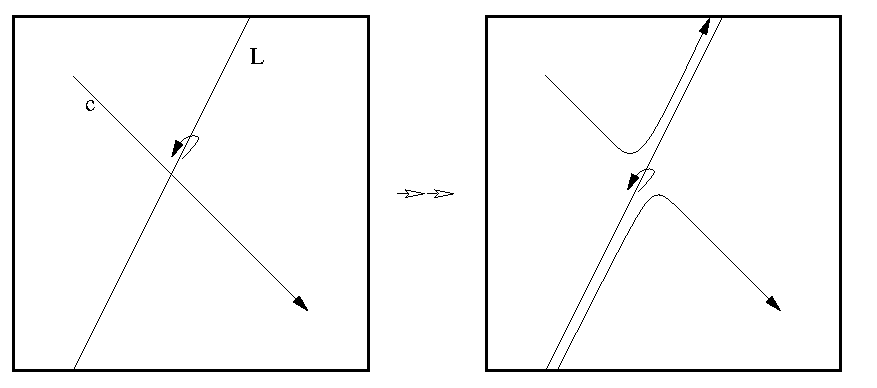
\includegraphics[width=0.62\textwidth]{figures/fig1.pdf}
  \caption{狄拉克弦与磁单极的磁场位形。(a) 磁荷 $g$ 位于原点，其磁场 $\vec{B}_{\rm mon}$ 沿径向向外；
           实心双线为狄拉克弦，其上携带回流磁通 $\vec{B}_{\rm sol}$。(b) 围绕狄拉克弦的闭合回路 $\Gamma$，
           用于计算沿回路的相位 $e\oint_\Gamma \vec{A}\cdot\mathrm{d}\vec{l}=eg$。原文仅标
           “Figure 1”（原文 PDF 第 7 页），无说明性图注；图注说明为译者据图补写。}
  \label{fig:1}
\end{figure}

\subsection{Georgi–Glashow 模型：一个有磁单极的简单理论}

到目前为止，我们一直在粒子力学的框架内工作，其中电荷与磁荷都是点状客体，并且是人为地引入理论中的。然而在场论中，这类客体也可以作为孤立子出现，即具有局域能量密度的场方程的非平凡解。如果与某孤立子解相联系的规范场位形具有磁性，该孤立子便可被认定为磁单极。最简单的孤立子出现在 Sine-Gordon 理论中，这是一个 $1+1$ 维的标量场论。然而，由 Derrick 定理，二维以上的标量场论不能支持静态有限能量解。这基本上是因为：孤立子在远距离处的非平凡结构使该位形的总能量发散。向理论中加入规范场可以弥补这一状况。因此，四维中含规范相互作用的标量理论可以容许静态有限能量的场位形。这类孤立子位形的稳定性往往与它们由守恒的拓扑荷所刻画这一事实有关。关于这些问题的更详细讨论，读者可参阅 \cite{GO, coleman1, coleman2}。下面我们描述 Georgi–Glashow 模型，这是一个 $3+1$ 维的、具有磁单极解的简单理论。

% [Tutor Note: 见原文 PDF 第 8 页“Derrick 定理”一句。原文只给结论，其证明是标度论证：对静态场作标度变换 $\phi_\lambda(\vec{x})=\phi(\lambda\vec{x})$，能量泛函可写成 $E(\lambda)=\lambda^{2-d}K+\lambda^{-d}V$（$K$ 为梯度项、$V$ 为势能项，均非负）；$d>1$ 时 $\mathrm{d}E/\mathrm{d}\lambda=0$ 无解，故 $d\ge2$ 的标量场论不存在静态有限能量解。原文另把这归因于孤立子在远距离处的非平凡结构，这是从位形角度的直观说法。]

Georgi–Glashow 模型是一个 Yang–Mills–Higgs 系统，它包含一个希格斯多重态 $\phi^a\,(a=1,2,3)$，它在规范群 $SO(3)$ 的伴随表示中按矢量变换，以及规范场 $W_\mu=W^a_\mu T^a$。这里，$T^a$ 是 $SO(3)$ 的厄米生成元，满足 $[T^a,T^b]=if^{abc}T^c$。在伴随表示中，有 $(T^a)_{bc}=-if^a_{bc}$；并且对 $SO(3)$ 而言 $f^{abc}=\epsilon^{abc}$。$W_\mu$ 的场强以及作用在 $\phi^a$ 上的协变导数定义为
\begin{eqnarray}
G_{\mu \nu} &=& \partial_{\mu}W_{\nu} - \partial_{\nu} W_{\mu} +
ie [W_{\mu},W_{\nu}]\,,
\nonumber\\
D_\mu\phi^a &=& \partial_\mu\phi^a - e\epsilon^{abc} W^b_\mu \phi^c\,.
\end{eqnarray}
最小拉格朗日量则为
\begin{equation}
{\cal L}  =  - \frac{1}{4} G^{a}_{\mu \nu} G^{a \mu \nu} +
\frac{1}{2} D^{\mu}\phi^a D_{\mu}\phi^a - V(\phi)\,,
\label{GGmodel}
\end{equation}
其中
\begin{equation}
V(\phi)=\frac{\lambda}{4}\left(\phi^2 - a^2 \right)^2\,.
\label{GGpot}
\end{equation}
由此拉格朗日量得到的运动方程为
\begin{equation}
(D_\nu G^{\mu \nu})^a=-e\,\epsilon^{abc}\,\phi^b\,(D^\mu\phi)^c,
\qquad D^\mu D_\mu \phi^a =-\lambda\phi^a (\phi^{2} - a^{2})\,. 
\label{XXIX}
\end{equation}
场强还满足比安基恒等式
\begin{equation}
D_\nu\,\widetilde G^{\mu \nu a} = 0\,.
\label{bianchi}
\end{equation}

% [Tutor Note: 见原文 PDF 第 8 页式 (15)、(16)。$W_\mu=W^a_\mu T^a$ 是矩阵值场，$G_{\mu\nu}=G^a_{\mu\nu}T^a$；用 $(T^a)_{bc}=-if^a_{bc}$ 与 $f^{abc}=\epsilon^{abc}$ 展开 $ie[W_\mu,W_\nu]$，得 $G^a_{\mu\nu}=\partial_\mu W^a_\nu-\partial_\nu W^a_\mu-e\epsilon^{abc}W^b_\mu W^c_\nu$。式中的因子 $i$ 与 $D_\mu\phi^a$ 里的 $-e$ 是配套的，符号弄反会直接改变式 (18) 的运动方程，并影响后文 BPS 界与磁荷的符号。]

我们来求该理论的真空位形。采用记号 $G_a^{0i}=-{\cal E}_a^i$ 与 $G_a^{ij} = -\epsilon^{ij}_
{\hphantom{ij}k}{\cal B}_a^k$，能量密度可写为
\begin{equation}
\theta_{00}=\frac{1}{2}\left(({\cal E}_a^i)^2+({\cal B}_a^i)^2 +
  (D^0\phi_a)^2 + ( D^i \phi_a)^2 \right) + V (\phi)\,.
\label{XXX}
\end{equation} 
注意 $\theta_{00} \geq 0$，并且它仅当下式成立时才为零：
\begin{equation}
G_{a}^{\mu \nu} = 0, \quad D_{\mu} \phi = 0, \quad V(\phi) = 0\,.
\label{XXXI}
\end{equation} 
第一个方程表明，在真空中 $W^a_\mu$ 是纯规范；后两个方程则定义了希格斯真空。真空空间的结构由 $V(\phi)=0$ 决定，其解为 $\phi^a= \phi^a_{vac}$，并满足 $|\phi_{vac}|=a$。因此，希格斯真空空间是场空间中半径为 $a$ 的二维球面（$S^2$）。为建立微扰论，我们必须选定其中一个真空，从而自发地破缺规范对称性（这就是通常的希格斯机制）。保持该真空不变的那部分对称性仍然保留下来，相应的未破缺生成元为 $\phi^c_{vac} T^c/a$。与该生成元相联系的规范玻色子是 $A_\mu=\phi^c_{vac}W^c_\mu/a$，而这一残存 $U(1)$ 的电荷算符由下式给出
\begin{equation} 
Q = \hbar e \frac{\phi^c_{vac}T^c}{a}\,.
\label{XXXIII}
\end{equation}
若群是紧致的，则该电荷是量子化的。理论的微扰谱可通过将 $\phi^a$ 在所选真空附近展开而得到：
$$
\phi^{a} = \phi^{a}_{vac} + \phi '^{a}\,.
$$
一个方便的选择是 $\phi^c_{vac}=\delta^{c3}a$。微扰谱（在选定适当规范后即显现）由一个有质量的希格斯粒子（$H$）、一个无质量光子（$\gamma$）和两个带电荷的有质量玻色子（$W^\pm$）组成；下表自左至右依次给出质量、自旋与电荷：
$$
\begin{tabular}{|c|c|c|c|}
\hline
& Mass & Spin & Charge \\
\hline
$H$ & $a(2\lambda)^{\frac{1}{2}} \hbar$ & $0$ &$0$ \\
\hline
$\gamma$ & $0$ & $\hbar$ & $0$ \\
\hline
$W^{\pm}$ & $ae\hbar = aq$ & $\hbar$ & $\pm q = \pm e \hbar$ \\
\hline
\end{tabular}
$$
下一节我们将考察 Georgi–Glashow 模型中磁单极（非微扰态）的存在性。

% [Tutor Note: 见原文 PDF 第 9 页微扰谱表格。表中“Spin”一列对光子与 $W^\pm$ 填 $\hbar$、对 $H$ 填 $0$，这是原文的写法：自旋一栏理应填自旋量子数 $1,1,0$（即 $s\hbar$ 中的 $s$），原文直接填入 $\hbar$，单位上亦不自洽，属原文笔误；为与源公式块保持一致，表头 Mass/Spin/Charge 保留原文，译名即“质量/自旋/电荷”。表中 $W^\pm$ 的质量 $ae\hbar=aq$ 与电荷 $\pm q=\pm e\hbar$ 彼此一致。]

% [Tutor Note: 本片原文拼写笔误汇总（译文均按正确词义翻译，源文件未改）：p2 “intented”→intended；p3 “proporties”→properties、“Minkowsky”→Minkowski；p4 “quations”→equations；p5 “elecromagnetic”→electromagnetic；p6 “fermios”→fermions，且“both of the components are bosonic.”句首小写；p7 “intruduced”→introduced；p8 “satifying”→satisfying、“representaion”→representation、“cavariant”→covariant。另有句读笔误一处，见式 (10) 前的批注。]
   % 引言、§1 与 §1.1--§1.4（原文 PDF 2--9 页）
%=====================================================================
%  分片 B：§1.5–§1.10（原文 PDF 第 9–22 页；原文印刷页 8–21）
%  底本：translate/src/src_B.tex；公式、编号、交叉引用逐字照录
%=====================================================================
% （本节重点见 §1 开头，由分片 A 负责）

\subsection{'t Hooft–Polyakov 磁单极}

我们在 Georgi–Glashow 模型中寻找不依赖时间、能量有限的解。能量有限要求：当 $r\rightarrow \infty$ 时，由 (\ref{XXX}) 给出的能量密度 $\theta_{00}$ 必须比 $1/r^3$ 更快地趋于零。这意味着当 $r\rightarrow \infty$ 时，我们的解必须过渡到由 (\ref{XXXI}) 定义的希格斯真空。下面我们先假定这样的有限能量解存在，并证明它可以带有与其孤子数相联系的磁单极荷，而孤子数又由相应的希格斯真空决定。这一结论的证明无需显式处理任何具体解。接下来，我们将介绍 't Hooft–Polyakov 拟设（ansatz），用以具体构造一个这样的磁单极解。我们还会评论双子（dyonic）解的存在性。为方便起见，本节中把矢量记号用于 $SO(3)$ 规范群指标，而不用于空间指标。

% [Tutor Note: 见原文 PDF 第 9 页开头。有限能量条件为 $E=\int\theta_{00}\,d^3x<\infty$：三维体积元带来 $r^2dr$，故要求 $\theta_{00}$ 的衰减快于 $1/r^3$（而不是快于 $1/r^2$）；这里的 $\theta_{00}$ 在静态情形下就是能量密度。]

\noindent\underline{磁荷的拓扑性质：}
\noindent 令 $\vec{\phi}_{vac}$ 表示处于希格斯真空中的场 $\vec{\phi}$。它满足方程
\begin{eqnarray}
&\vec{\phi}_{vac}\cdot\vec{\phi}_{vac} = a^2\,, &\nonumber \\
&\partial_{\mu} \vec{\phi}_{vac}-e\,\vec{W}_{\mu} \times
\vec{\phi}_{vac} = 0\,,& 
\label{vec-vac}
\end{eqnarray}
由此可解出 $\vec{W}_\mu$。最一般的解为
\begin{equation}
\vec{W}_{\mu} = \frac{1}{ea^{2}}\, \vec{\phi}_{vac} \times
\partial_\mu\vec{\phi}_{vac}+\frac{1}{a}\vec{\phi}_{vac}A_{\mu}\,.
\label{sol-vac}
\end{equation}
% [Tutor Note: 见原文 PDF 第 10 页式 (24)。此处系数最容易写错：第一项的 $1/(ea^2)$ 中 $a^2$ 来自 $\vec{\phi}_{vac}\cdot\vec{\phi}_{vac}=a^2$，第二项的 $1/a$ 保证 $A_\mu$ 是归一化的 $U(1)$ 规范场。代回式 (23) 时只需两个恒等式：$\vec{\phi}_{vac}\cdot\partial_\mu\vec{\phi}_{vac}=0$ 与 $(\vec{\phi}_{vac}\times\partial_\mu\vec{\phi}_{vac})\times\vec{\phi}_{vac}=a^2\partial_\mu\vec{\phi}_{vac}$。]
为看出它确实满足 (\ref{vec-vac})，注意 $\partial_\mu\vec{\phi}_{vac}\cdot\vec{\phi}_{vac}=0$，于是
$$
\frac{1}{ea^2}(\vec{\phi}_{vac}\times\partial_{\mu}\vec{\phi}_{vac})
\times \vec{\phi}_{vac}= \frac{1}{ea^2}\left(\partial_\mu\vec{\phi}_{vac}a^2
-\vec{\phi}_{vac} (\vec{\phi}_{vac}\cdot\partial_\mu\phi_{vac})\right)= 
\frac{1}{e}\partial_\mu\vec{\phi}_{vac}\,.
$$
式 (\ref{sol-vac}) 右端第一项是特解，而 $\vec{\phi}_{vac}A_\mu$ 是齐次方程的通解。利用这个解，我们现在可以计算场强张量 $\vec{G}_{\mu\nu}$。对应于规范群未破缺部分的场强 $F_{\mu\nu}$ 可确定为
\begin{eqnarray}
F_{\mu\nu}&=&\frac{1}{a}\vec{\phi}_{vac}\cdot\vec{G}_{\mu \nu}
\nonumber\\
&=&\partial_\mu A_\nu -\partial_\nu A_\mu +
\frac{1}{a^3 e}\vec{\phi}_{vac}\cdot (\partial_\mu\vec{\phi}_{vac}
\times\partial_\nu\vec{\phi}_{vac})\,.
\label{F-vac}
\end{eqnarray}
利用希格斯真空中的运动方程可得
$$
\partial_\mu F^{\mu\nu}=0\,,\qquad \partial_\mu\,\widetilde F^{\mu\nu}=0\,.
$$
这证实 $F_{\mu\nu}$ 是一个合法的 $U(1)$ 场强张量。磁场由 $B^i=-\frac{1}{2}\epsilon^{ijk}F_{jk}$ 给出。现在考虑一个静态、能量有限的解，以及一个包围该解核心的曲面 $\Sigma$。我们取 $\Sigma$ 足够远，使其上解已处于希格斯真空中。于是可以用希格斯真空中的磁场来计算与该解相联系的磁荷 $g_\Sigma$：
\begin{equation}
g_\Sigma=\int_\Sigma\,B^i ds^i=-\frac{1}{2 ea^3} \int_\Sigma\, 
\epsilon_{ijk}\,\vec{\phi}_{vac}\cdot \left(\partial^j\vec{\phi}_{vac}
\times\partial^k\vec{\phi}_{vac}\right)ds^i\,.
\label{XL}
\end{equation}
下面说明右端的表达式是一个拓扑量：由于 $\phi^2=a$，希格斯真空的流形（${\cal M}_0$）具有 $S^2$ 的拓扑。
% [Tutor Note: 原文笔误，见原文 PDF 第 10 页式 (26) 之后。“Since $\phi^2=a$;”有两处问题：(1) 应为 $\phi^2=a^2$，与式 (23) 一致；(2) 分号应为逗号。译文照录公式原样，只按文意断句。]
场 $\vec{\phi}_{vac}$ 定义了从 $\Sigma$ 到 ${\cal M}_0$ 的映射。由于 $\Sigma$ 也是 $S^2$，映射 $\phi_{vac}:\Sigma\rightarrow{\cal M}_0$ 由其同伦群 $\pi_2 (S^2)$ 刻画。换言之，$\phi_{vac}$ 由一个整数 $\nu$（绕数）刻画，它计算该映射把 $\Sigma$ 缠绕到 ${\cal M}_0$ 上的次数。用映射 $\phi_{vac}$ 表示，这个整数为
\begin{equation}
\nu = \frac{1}{4\pi a^{3}} \, \int_\Sigma\,\frac{1}{2}
\epsilon_{ijk}\vec{\phi}_{vac}\cdot\left(\partial^j\vec{\phi}_{vac}
\times \partial^k\vec{\phi}_{vac}\right)\,d s^i\,.
\label{XLI}
\end{equation}
与磁荷的表达式比较，我们得到重要结果
\begin{equation}
g_{\Sigma} = - \frac{4\pi \nu}{e}\,.
\label{XLII}
\end{equation}
% [Tutor Note: 见原文 PDF 第 10 页式 (28)。原文说它与狄拉克条件“相差因子 2”，核对如下：取 $q_0=e\hbar/2$，则 $g_\Sigma q_0/(4\pi\hbar)=-\nu/2$，而狄拉克条件为 $qg/(4\pi\hbar)=n/2$，故要求 $\nu=-n$。式 (26) 中的负号来自 $B^i=-\frac{1}{2}\epsilon^{ijk}F_{jk}$ 与曲面定向的约定，不要与式 (27) 中 $\nu$ 的符号约定混为一谈。]
因此，孤子的绕数决定它的磁单极荷。注意上式与狄拉克量子化条件相差一个因子 $2$。这是因为本模型中可能存在的最小电荷是 $q_0=e\hbar/2$，用它可把 (\ref{XLII}) 化为狄拉克条件。

\noindent\underline{磁单极的拟设：}
\noindent 现在我们介绍 't Hooft \cite{thooft} 与 Polyakov \cite{polya} 提出的拟设，用于在 Georgi–Glashow 模型中构造磁单极解。对于球对称、宇称不变、静态且能量有限的解，他们提出：
\begin{eqnarray}
\phi^a & = & \frac{x^a}{er^2}\,H(aer)\,,\nonumber\\
W^a_i&=&-\epsilon^a_{ij}\frac{x^j}{er^2}\left(1 - K(aer)\right)\,,
\qquad W^a_0= 0\,.
\label{tp-ansatz}
\end{eqnarray}
对于 $r\rightarrow\infty$ 处的非平凡希格斯真空，他们取 $\phi^c_{vac}=ax^c/r= a\hat{x}^c$。注意这把空间无穷远处的 $S^2$ 映到真空流形上，绕数为 1。函数 $H(aer)$ 与 $K(aer)$ 的渐近行为由 $r\rightarrow\infty$ 时的希格斯真空以及 $r=0$ 处的正则性决定。具体地，定义 $\xi=aer$，我们有：当 $\xi\rightarrow\infty,\,H\sim\xi,\, K\rightarrow 0$，当 $\xi\rightarrow 0,\, H\sim\xi,\,(K-1)\sim\xi$。该解的质量可参数化为
$$
M = \frac{4 \pi a}{e} f \, (\lambda /e^{2})
$$
% [Tutor Note: 见原文 PDF 第 11 页式 (29) 之后。核对边界条件：$r\to0$ 时 $H\sim\xi$ 使 $\phi^a=(x^a/er^2)H\to c_1x^a\to0$，故场在原点正则；$r\to\infty$ 时 $H\sim\xi$ 给出 $\phi^a\to ax^a/r=a\hat{x}^a$，而 $K\to0$ 给出 $W^a_i\to-\epsilon^a_{ij}x^j/er^2$。注意 $H$、$K$ 的自变量是 $\xi=aer$ 而不是 $r$，做量纲核对时不要丢掉 $e$ 与 $a$。]
对该拟设，运动方程约化为关于 $K$ 与 $H$ 的两个耦合方程，它们只在某些极限下才能精确求解。当 $r\rightarrow 0$ 时，得到 $H\rightarrow ec_1 r^2$ 与 $K=1+ec_2r^2$，这表明场在 $r=0$ 处不奇异。当 $r\rightarrow\infty$ 时，我们得到 $H\rightarrow\xi+c_3 exp(-a\sqrt{2\lambda}r)$ 与 $K\rightarrow c_4\xi exp(-\xi)$，从而 $W^a_i\approx-\epsilon^a_{ij}x^j/er^2$。再次定义 $F_{ij}=\phi^c G^c_{ij}/a$，磁场为 $B^{i} = - x^i/e r^3$。相应的磁单极荷为 $g=-4\pi/e$，这与该解的绕数为 1 所预期的一致。应当指出，'t Hooft 对阿贝尔场强张量的定义略有不同，但在大距离下它化为上述形式。

注意在上述磁单极解中，狄拉克弦的出现并不显然。为了把狄拉克弦提取出来，我们必须对该解作一个奇异规范变换，把非平凡的希格斯真空 $\phi^c_{vac}=a\hat{x}^c$ 旋转为平庸真空 $\phi^c_{vac}= a \delta^{c3}$。在此过程中，规范场产生了狄拉克弦奇点，它现在充当磁荷的源 \cite{thooft}。

\noindent\underline{Julia–Zee 双子：}

't Hooft–Polyakov 磁单极携带一个单位的磁荷，不带电荷。Georgi–Glashow 模型也允许既带磁荷又带电荷的解。构造这类解的一个拟设由 Julia 与 Zee \cite{Julia-Zee} 提出。在该拟设中，$\phi^a$ 与 $W^a_i$ 的形式与 't Hooft–Polyakov 拟设完全相同，但 $W^a_0$ 不再为零：$W^a_0=x^a J(aer)/er^2$。它充当双子电荷的源。双子的电荷依赖于一个连续参数，在经典层次上并不满足量子化条件。然而，半经典论证 \cite{TW1,GSW} 表明，在 CP 不变的理论中，在量子层次上，双子的电荷量子化为 $q=n\hbar e$。只要认识到磁单极在规范变换下并非不变（而规范变换当然是运动方程的对称性），这一点就很容易理解。为正确处理相应的零模，应把规范自由度视为集体坐标。经过量子化，这个集体坐标导致磁单极存在带离散电荷的带电态。当拉格朗日量中存在破坏 CP 的项时，情况更为微妙，我们将在后面讨论。在下一小节中，我们将描述一个极限，在其中 't Hooft–Polyakov 与 Julia–Zee 拟设的运动方程可以精确求解。这就是孤子质量达到 Bogomol'nyi 界饱和的极限。
% [Tutor Note: 原文 PDF 第 11 页这一段有数处拼写笔误：“easiy”应为“easily”，“guage”应为“gauge”，“treate”应为“treat”，“depends of”应为“depends on”；译文均按原意处理。关于集体坐标论证：静态双子解带有一个连续参数（即 $W^a_0$ 的系数），它对应于保持希格斯真空的 $U(1)$ 规范方向的零模；把该规范自由度作为集体坐标量子化后，其共轭动量（电荷）取分立值 $q=n\hbar e$，细节见文献 [12,13]。]

\subsection{Bogomol'nyi 界与 BPS 态}

本小节中，我们导出双子质量上的 Bogomol'nyi 界 \cite{bogomol}，用其电荷与磁荷（它们是 $F^{\mu\nu}=\vec{\phi}\cdot \vec{G}^{\mu\nu}/a$ 的源）来表示。利用比安基恒等式 (\ref{bianchi}) 以及 (\ref{XXIX}) 中的第一个方程，可把这些荷写成
\begin{eqnarray} 
g&\equiv&\int_{S^2_\infty}B_i dS^i=\frac{1}{a}\int{\cal B}^a_i\phi^a
dS^i = \frac{1}{a} \int {\cal B}^a_i (D^i \phi)^a d^3x\,,
\nonumber\\
q&\equiv&\int_{S^2_\infty}E_i dS^i=\frac{1}{a}\int{\cal E}^a_i\phi^a
dS^i = \frac{1}{a} \int {\cal E}^a_i (D^i \phi)^a d^3x\,. 
\label{gq}
\end{eqnarray}
% [Tutor Note: 见原文 PDF 第 12 页式 (30)。把面积分化为体积分用了两个不同方程：磁荷用非阿贝尔比安基恒等式 $D_i{\cal B}^a_i=0$，电荷用高斯定律（即 (\ref{XXIX}) 的第一个方程）。注意等号链中“面积分”与“体积分”之间的那一步并不只是把 $a$ 提出：需要把 $\phi^a/a$ 作为单位矢量场、分部积分并用 $D_i{\cal B}^a_i=0$，才能把被积函数中的 $\phi^a$ 换成 $(D^i\phi)^a$；这是本节最容易被读者一带而过的地方。]
现在，在质心系中，双子的质量由下式给出
$$
M\equiv \int d^3x \theta_{00}= \int d^3x \left(\,\frac{1}{2}
\left[({\cal E}^a_k)^2+({\cal B}^a_k)^2 + (D_k\phi^a)^2 + 
(D_0\phi^a)^2 \right]+ V(\phi) \right)\,,
$$
其中 $\theta_{\mu\nu}$ 是能量动量张量。稍加运算，并利用 (\ref{gq}) 中给出的电荷与磁荷表达式，可把它写成
\begin{eqnarray}
M&=&\int d^3x \left(\,\frac{1}{2}\left[({\cal E}^a_k -
D_k\phi^a\sin\theta)^2 + ({\cal B}^a_k-D_k\phi^a\cos\theta )^2
+(D_0\phi^a)^2\right] + V(\phi) \right)
\nonumber\\
&+& a (q \sin \theta + g \cos \theta )\,,
\label{M-bog}
\end{eqnarray}
% [Tutor Note: 易错预警，见原文 PDF 第 12 页式 (31)。平方配方时务必与式 (30) 中 $g,q$ 的定义对照：把方括号内展开，除保留 $\frac12[({\cal E}^a_k)^2+({\cal B}^a_k)^2+(D_k\phi^a)^2+(D_0\phi^a)^2]$ 外，交叉项为 $-\sin\theta\,{\cal E}\cdot D\phi-\cos\theta\,{\cal B}\cdot D\phi=-a(q\sin\theta+g\cos\theta)$（注意是负号！），移项后才得到式 (31) 末行的 $+a(q\sin\theta+g\cos\theta)$。若把交叉项符号弄反，就会得出 $M\le a\sqrt{q^2+g^2}$ 的错误结论。对 $\theta$ 求极值时用 $\tan\theta=q/g$，最大值为 $\sqrt{q^2+g^2}$。]
其中 $\theta$ 是任意角。由于第一行中的各项为正，我们可以写出 $M\geq (q \sin \theta + g \cos \theta )$。该界在 $\tan\theta = q/g$ 时取最大。于是得到双子质量上的 Bogomol'nyi 界
$$
M \geq a\, \sqrt{g^2 + q^2}\,.
$$
对 't Hooft–Polyakov 解，我们有 $q = 0$，因此 $M \geq a|g|$。但 $|g|=4\pi/e$，且 $M_W=ae\hbar=aq$，所以
$$
M \geq a \frac{4 \pi}{e} = \frac{4 \pi}{e^{2}\hbar} M_{W} =
\frac{4 \pi \hbar}{q^{2}} M_{W} = \frac{\nu}{\alpha} M_{W}\,.
$$
这里 $\alpha$ 是精细结构常数，$\nu=1$ 或 $1/4$，取决于电子电荷取 $q$ 还是 $q/2$。由于 $\alpha$ 是一个很小的数（对电磁相互作用 $\sim 1/137$），上述关系意味着磁单极远比与对称性破缺相联系的 W 玻色子重。
% [Tutor Note: 见原文 PDF 第 12 页。此处对 $\hbar$ 的处理较随意：由 $M_W=ae\hbar=aq$ 与 $\nu/\alpha$ 的写法可反推出 $\alpha\equiv q^2/(4\pi\hbar)$，只有取 $\hbar=1$ 时才与通常的 $\alpha=e^2/4\pi\sim1/137$ 相符。原文此处只作定性结论（磁单极远重于 W 玻色子），不必纠结 $\hbar$ 的幂次；$\nu=1$ 或 $1/4$ 则取决于把“电子电荷”取作 $q$ 还是 $q/2$。]
由 (\ref{M-bog}) 可见，除非 $\lambda\rightarrow 0$ 使 $V(\phi)=0$，否则界不会饱和。这就是理论的 Bogomol'nyi–Prasad–Sommerfield（BPS）极限 \cite{bogomol,PS}。注意在此极限下，$\phi_{vac}^2 =a^2$ 不再由理论决定，因此必须作为希格斯场的边界条件加上。此外，在此极限下希格斯标量变为无质量。现在，为使界饱和，我们必须取
\begin{equation}
D_0 \phi^a=0\,,\qquad {\cal E}^a_k=(D_k\phi)^a\sin\theta\,,
\qquad{\cal B}^a_k = (D_k\phi)^a\cos\theta\,,
\label{L}
\end{equation}
其中 $\tan\theta=q/g$。在 BPS 极限下，可以在 (\ref{XXIX}) 中或在 (\ref{L}) 中使用 't Hooft–Polyakov（或 Julia–Zee）拟设，从而得到精确的磁单极（或双子）解 \cite{bogomol, PS}。这些解自动达到 Bogomol'nyi 界，被称为 BPS 态。还要注意，在 BPS 极限下，理论的所有微扰激发都达到该界，因而属于 BPS 谱。我们将在后面看到，在 $N=2$ 超对称理论中 BPS 界以非常自然的方式出现。
% [Tutor Note: 见原文 PDF 第 13 页。式 (32) 其实是两类一阶（BPS）方程的合写：$D_0\phi=0$ 与 $\vec{\cal E}=\sin\theta\,D\phi$、$\vec{\cal B}=\cos\theta\,D\phi$；把 't Hooft–Polyakov 拟设代入这些一阶方程即可精确求解（原文引 [14,15]）。另注意：$\lambda\to0$ 时 $V=0$，$a$ 不再由势的极小值固定，故 $|\phi|=a$ 只能作为边界条件强加，这一点在后文 Seiberg–Witten 分析中至关重要。]

\subsection{远距离下的磁单极}

迄今为止，我们都是从理论的希格斯真空结构出发来描述 Georgi–Glashow 模型中产生的磁单极。本节将考虑一般杨–米尔斯–希格斯系统中的磁单极，并把希格斯真空的描述与用未破缺规范场给出的描述联系起来。这些规范场保持无质量，是研究大距离下磁单极时相关的场。这种表述便于描述非阿贝尔磁单极。

设 $\phi$ 按规范群 $G$ 的某个给定表示中的矢量变换。为记号方便，下文我们不再区分群元素 $g$ 与它的某一具体实现。把规范场写成 $W_\mu=T^aW^a_\mu$，我们可以构造 $\phi$ 的协变导数与 $W_\mu$ 的曲率张量如下
\begin{eqnarray}
D_\mu \phi &=& \partial_{\mu} \phi + ie W_{\mu} \phi\,,
\nonumber \\
G_{\mu\nu}&=&\partial_\mu W_\nu -\partial_\nu W_\mu +
ie [W_\mu, W_\nu] \,.
\nonumber
\end{eqnarray}
% [Tutor Note: 术语与记号说明，见原文 PDF 第 13 页。原文用同一个字母 $g$ 表示两件完全不同的东西：群元素 $g$（如式 (36) 的 $g(s,t)$）与磁荷 $g$（见式 (30) 与式 (35)）。阅读时须按上下文区分，切勿把 $g(s,t)$ 的指标结构套到磁荷上。]
拉格朗日密度 ${\cal L}$、能量动量张量 $\theta_{\mu\nu}$ 与规范流 $j^a_\mu$ 则如下给出
\begin{eqnarray}
{\cal L}&=&-\frac{1}{4}(G^a_{\mu\nu})^2+(D^\mu\phi)^\dagger D_\mu\phi
-V(\phi) \,,
\nonumber\\
\theta_{\mu\nu}&=&-G^a_{\mu\lambda}G^{a\lambda}_\nu +
(D_\mu\phi)^\dagger(D_\nu\phi) + (D_\nu\phi)^\dagger(D_\mu\phi) 
- g_{\mu\nu} {\cal L} \,,
\nonumber \\
\theta_{00}&=& \frac{1}{2}{\cal E}^{ia}{\cal E}^a_i +
\frac{1}{2}{\cal B}^{ia}{\cal B}^a_i +D_0\phi^\dagger D_0\phi +
D_i\phi^\dagger D_i\phi + V(\phi)\,,
\nonumber \\
j^a_\mu &=& ie \phi^\dagger T^a D_\mu\phi -
ie (D_\mu\phi)^\dagger T^a \phi\,.
\label{LIII}
\end{eqnarray}
这里希格斯势是规范不变的：$V(g\phi)=V(\phi)$。由上述拉格朗日量得到的运动方程为
\begin{equation}
D^\mu D_\mu\phi^a=-\frac{\partial V}{\partial \phi^a}\,,\qquad
D^\nu G^a_{\mu\nu} = - j_\mu^a\,.
\label{LIV}
\end{equation}
当规范群 $SO(3)$ 自发破缺到 $U(1)$ 时，我们可以像上一节那样精确算出 Bogomol'nyi 界，结果为
\begin{equation}
M\geq \sqrt 2 \, a \sqrt{g^2 + q^2}\,.
\label{Bbound}
\end{equation}
% [Tutor Note: 易错预警，见原文 PDF 第 14 页式 (35)。与 §1.6 的 $M\ge a\sqrt{g^2+q^2}$ 相比这里多出因子 $\sqrt2$：式 (33) 的希格斯动能是复标量的 $(D_\mu\phi)^\dagger D^\mu\phi$，平方配方时须写成 $\frac{1}{2}|{\cal E}-\sqrt2\,D\phi\sin\theta|^2$、$\frac{1}{2}|{\cal B}-\sqrt2\,D\phi\cos\theta|^2$ 之类的形式（实部、虚部各贡献一份），交叉项才给出 $\sqrt2\,a(q\sin\theta+g\cos\theta)$；若照搬 §1.6 实伴随场的 $\frac12(D\phi)^2$ 配方，就会漏掉这个 $\sqrt2$。]
对一般的规范群 $G$，如 Georgi–Glashow 模型那样，希格斯真空由下式定义
$$
V(\phi)=0\,,\qquad D_\mu\phi=0 \,.
$$
第一个方程定义了真空流形 ${\cal M}_0\equiv \{\phi\,: V(\phi)=0\}$，第二个方程给出
$$
[D_\mu, D_\nu] \phi =G_{\mu\nu} \phi = 0\,. 
$$
因此，在希格斯真空中，$G_{\mu\nu}$ 取值于规范群 $G$ 中保持希格斯真空不变的某个子群。我们用 $H$ 表示 $G$ 的这个未破缺子群。$G$ 中不保持希格斯真空不变的生成元当然被破缺，相应的规范玻色子获得质量。如果 $V(\phi)$ 没有额外的整体对称性与偶然的极小值，那么可以合理地假定 $G$ 在 ${\cal M}_0$ 上的作用是传递的。这意味着 ${\cal M}_0$ 中任一点都可通过 $G$ 的某个元素与任意另一点（特别是与某个参考点 $\phi_0$）相联系。因此，${\cal M}_0$ 中任一点的小群（不变群）$H\subset G$ 都同构于其他任一点的小群。于是 ${\cal M}_0$ 的结构由右陪集 $G/H$ 描述。
% [Tutor Note: 含糊点拨，见原文 PDF 第 14 页。原文“$G_{\mu\nu}$ 取值于 $G$ 的某个子群”严格说应为“取值于该子群的李代数”；这里只是省略了“李代数”三字，物理内容不变。又：原文此处有重复词 “the the little group”，系笔误。]
为使解具有有限能量，在离解核心足够远处，场 $\phi$ 必须取值于希格斯真空中。设 $\Sigma$ 是包围核心的一个二维曲面，使得在它上面 $\phi$ 已处于 ${\cal M}_0$ 中。在此曲面上，$\phi$ 描述一个从 $\Sigma$（具有 $S^2$ 的拓扑）到 ${\cal M}_0$ 的映射。该映射由其同伦类刻画，同伦类必须是 $\pi_2({\cal M}_0)\simeq \pi_2(G/H)$ 的一个元素。如前所述，相应的拓扑数就是解的磁荷。只要没有磁单极穿过曲面 $\Sigma$，$\phi$ 就保持为时间的连续函数，其同伦类不变。要证明映射 $\phi$ 满足 $\pi_2(G/H)$ 的群性质，必须考虑若干彼此远离的磁单极，并研究它们的磁荷如何合成。关于这一问题的讨论见 \cite{coleman1}。

以上关于磁单极拓扑刻画的讨论是基于希格斯真空的结构。然而，用未破缺规范场来描述更为自然。这两种描述之间的关系包含在方程 $D_\mu\phi =0$ 之中，该方程在 $S^2$ 曲面 $\Sigma$ 上成立。让我们用正方形 $\{ 0 \leq s, t \leq 1 \}$ 来参数化 $S^2$。从这个正方形到球面的映射 $r(s,t)$ 除在正方形的边界上外处处单值，而该边界被等同于球面上的一个点：
% [Tutor Note: 原文笔误，见原文 PDF 第 14 页：“from this square to the sphare” 中 “sphare” 应为 “sphere”。]
$$
r(0,t) = r(1,t) =r(s,0) =r(s,1) = r_0\,.
$$
固定 $s$ 时，当 $t$ 从 $0$ 变到 $1$，$r(s,t)$ 描述 $S^2$ 上的一条闭路径。

\begin{figure}[htbp]
  \centering
  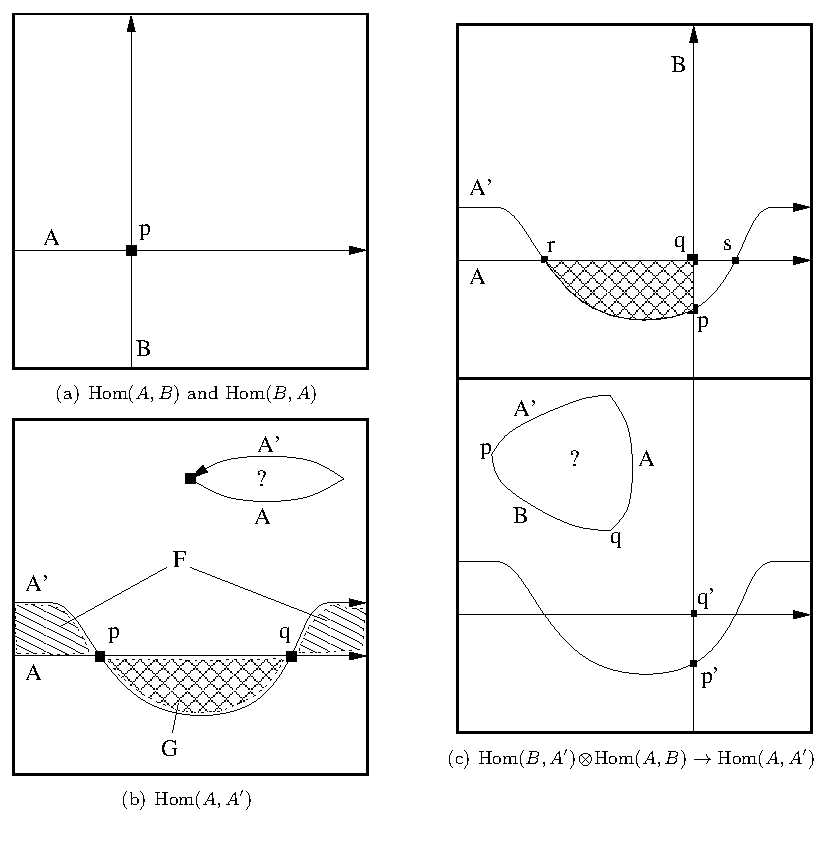
\includegraphics[width=0.92\textwidth]{figures/fig2.pdf}
  \caption{二维球面 $S^2$ 上闭曲线的同伦类。(左) 参数域 $(s,t)\in[0,1]^2$，边界整体映为基点 $r_0$，
           竖直箭头表示 $t$ 增大方向；(右) 球面 $\Sigma$ 上对应的闭曲线族，均自基点 $r_0$ 出发并回到 $r_0$。
           原文仅标 “Figure 2”（原文 PDF 第 15 页），无说明性图注。}
  \label{fig:2}
\end{figure}
% [Tutor Note: 图 2 的读法，见原文 PDF 第 15 页。$(s,t)$ 正方形的整个边界都映到基点 $r_0$，故对每个固定的 $s$，$t\in[0,1]$ 是 $\Sigma$ 上一条由 $r_0$ 出发又回到 $r_0$ 的闭曲线；右图中这些闭曲线按同伦类分层，其绕数即磁荷。注意左图中竖直箭头只表示 $t$ 增大方向，图中的“曲线族”是同一映射 $r(s,t)$ 在不同 $s$ 处的像。]

沿 $t$ 方向的协变导数为
$$
D_t \phi(s,t) =\frac{\partial r^i}{\partial t}D_i \phi(s,t)=0\,.
$$
对常数 $s$，可把它解出为
$$
\phi(s,t)=g(s,t)\phi(s,0)\,, 
$$
其中 $g(s,t)$ 满足 $D_t g=0$、$g(s,0)=1$，并由路径编序积分给出
\begin{equation}
g (s,t) =  P\left(\,\exp \left(\,ie\int^{t}_{0}
\vec{W}\cdot\frac{\partial \vec{r}}{\partial t} \, dt\right)\right)\,. 
\label{LVIII}
\end{equation}
% [Tutor Note: 见原文 PDF 第 15 页式 (36)。$P$ 表示路径编序（沿 $t$ 增大方向）；指数中 $ie\int\vec{W}\cdot d\vec{r}$ 的量纲须与式 (33) 的 $D_\mu=\partial_\mu+ieW_\mu$ 一致，核对时勿额外添加 $e$ 或 $2\pi$。]
显然，$g(s,t)$ 是 $G$ 的一个元素，它通过规范变换把任意 $\phi(s,t)$ 变到参考值 $\phi(s,0)$，而 $\phi(s,0)=\phi_0$ 与 $s$ 无关。因此，$g(s,t)$ 包含与 $\phi(s,t)$ 相同的拓扑信息，并由 $\pi_2(G/H)$ 中的一个同伦类刻画。由于在 $s=0,1$ 处 $\partial r/ \partial t =0$，故 $g(0,t)=g(1,t)=1$。当 $t=1$ 时，$\phi(s,1)=g(s,1)\phi_0$。但由于 $\phi(s,1)=\phi_0$，我们断定 $g(s,1)$ 必为未破缺规范群 $H$ 的元素，并把它记为 $h(s)$：
\begin{equation}
h(s)\equiv g(s,1)=P\,\exp\left(ie\int^1_0\,\vec{W}\cdot\frac{\partial
\vec{r}}{\partial t}\,dt\right)\,. 
\label{LIX}
\end{equation}
由于 $h(1)=h(0)=1$，当我们沿 $s$ 移动时，$h(s)$ 描述 $H$ 中的一条闭路径，因而属于 $\pi_1(H)$。然而要注意，当 $t$ 从 $1$ 变到 $0$ 时，$g(s,t)$ 在 $h(s)$ 与恒等元之间连续插值。因此，$h(s)$ 只能描述 $H$ 中那些在 $H$ 嵌入 $G$ 后同伦于平庸路径的闭路径。我们把 $\pi_1(H)$ 中对应于这类路径的子群记为 $\pi_1(H)_G$。若映射 $\phi(s,t)$ 的同伦类在 $\pi_2(G/H)$ 中改变，则 $h(s)$ 的同伦类在 $\pi_1(H)_G$ 中改变。事实上，$\pi_2(G/H)$ 与 $\pi_1(H)_G$ 之间存在一一对应，两个群同构 \cite{coleman1}。于是，我们同样可以用其在 $\pi_1(H)_G$ 中的同伦类来刻画磁单极。

让我们更详细地讨论这一点。由于 $H$ 中的任何闭路径也是 $G$ 中的闭路径，存在从 $\pi_1(H)$ 到 $\pi_1(G)$ 的自然同态。如上文讨论所示，$\pi_1(H)_G$ 位于该同态的核中。此外，对紧致连通群 $G$，$\pi_2(G)=0$，这意味着 $\pi_2(G)$ 可作为单位元嵌入 $\pi_2(G/H)$。我们上面所做的，基本上是构造了如下正合序列的一部分：
$$
\pi_2(G)\rightarrow\pi_2(G/H)\rightarrow\pi_1(H)\rightarrow 
\pi_1(G)\rightarrow\pi_1(G/H)\rightarrow\pi_0(H)
$$
% [Tutor Note: 含糊点拨，见原文 PDF 第 16 页的正合序列。原文“$\pi_2(G)$ 可作为单位元嵌入 $\pi_2(G/H)$”的措辞不严谨：对紧致连通 $G$ 有 $\pi_2(G)=0$，于是由正合性得 $\pi_2(G/H)$ 单射地映入 $\pi_1(H)$，其像正是（在 $G$ 中同伦于平庸路径的）$\pi_1(H)_G$，故 $\pi_2(G/H)\cong\pi_1(H)_G$。原文所谓“嵌入”只是说明 $\pi_2(G)=0$ 这一环在序列中不贡献，读者不必按字面理解为群嵌入。完整讨论见文献 [2]（Coleman）。]
注意若 $G$ 单连通，则 $\pi_1(G)=0$ 且 $\pi_1(H)_G=\pi_1(H)$，于是整个 $\pi_1(H)$ 都进入磁单极的物理描述。对非单连通的 $G$，这种情况可以在存在狄拉克弦时实现。这样的弦表现为 $(s,t)$ 平面上的一个奇点；在它存在时，不再能把 $h(s)$ 连续形变到恒等映射。因此 $h(s)$ 的同伦类不再受限于 $\pi_1(H)_G$。然而，对非单连通的 $G$，只要把 $G$ 嵌入其万有覆盖群 $\tilde G$，仍可用不受限制的 $\pi_1$ 群来描述。我们用 $\hat H$ 表示 $\phi$ 的小群。由于 $\tilde G$ 必定连通，$\pi_1(\tilde G)=0$ 且 $\pi_1(\hat H)= \pi_1(H)_G$。作为例子，考虑 Georgi–Glashow 模型。这里 $G = SO(3)$（其中 $(Ta)_{ij}=-i\epsilon_{aij}$），$\tilde{G} = SU(2)$（其中 $T_a=\frac{1}{2}\sigma_a$）。$H$（或 $\hat H$）中同伦不等价的路径为：
$$
h(t)=\exp(it\,\vec{\phi}\cdot\vec{T}\,4\pi N/a),\quad {\rm for}\,\,\, 
0 \leq t \leq 1\,.
$$
刻画 $\pi_1$ 中元素的整数 $N$ 如下确定：
$$
\begin{array}{llll}
\tilde G=SU(2),& \tilde H=U(1),& \vec{\phi}\cdot\vec{T}\in 
\frac{1}{2}{\bf Z},& \Rightarrow\,\, N \in {\bf Z}\,, \cr
G=SO(3),& H=SO(2),& \vec{\phi}\cdot\vec{T}\in {\bf Z},&
\Rightarrow\,\, N \in \frac{1}{2}{\bf Z}\,.
\end{array}
$$
由于 $SO(3)\sim S^2/{\bf Z}_2$，两种情形下都只有整数 $N$ 的路径有贡献。后面我们会证明 $g=4\pi N/e$。对 $SU(2)$，$q_0=e\hbar/2$ 且 $gq_0/4\pi\hbar=N/2$；对 $SO(3)$，$q_0=e\hbar$ 且 $gq_0/4\pi\hbar=N$。
% [Tutor Note: 见原文 PDF 第 16 页。原文称“后面我们会证明 $g=4\pi N/e$”，但本分片后文并未再给出独立证明；读者可对照式 (37)–(42) 的广义量子化条件自行补出（比较 $h(t)$ 的指数中 $4\pi N/a$ 的归一化与式 (41) 中 $G_0$ 前的 $ie/4\pi$）。另注意半整数 $N$ 的路径在 $SO(3)$ 中虽闭合，却生成 $\pi_1(SO(3))={\bf Z}_2$ 的非平凡类，不在 $\pi_1(H)_G$ 中，故最终两种情形都只保留整数 $N$。]

对 Glashow–Weinberg–Salam 模型，$G=SU(2)\times U(1)$，$H=U(1)$ 是 $SU(2)$ 与 $U(1)$ 的线性组合。虽然 $\pi_{1} (H) = {\bf Z}$，但 $\pi_{1} (H)_{G} = 0$。因此在该模型中，任何非平凡磁单极都必须带有狄拉克弦。

我们的目标是只用未破缺规范场（$H$ 场）来描述磁单极。虽然已经得到了用 $\pi_1(H)_G$ 的表述，但由 (\ref{LIX}) 给出的 $h(s)$ 只涉及 $H$ 场这一点并不显然。下面来说明：量 $g^{-1}(s,t)D_s g(s,t)$ 在依赖于 $t$ 的规范变换下不变。此外，由构造 $D_t g(s,t)=0$。因此可以写出
\begin{equation}
\partial_t(g^{-1}D_s g)= D_t(g^{-1}D_s g)=g^{-1}[D_t,D_s] g =
ie g^{-1} G_{ij} g \frac{\partial r^i}{\partial t} \frac{\partial r^j}
{\partial s}\,.
\label{LX}
\end{equation}
把上式的第一项与最后一项从 $t=0$ 积分到 $t=1$。由于 $t=0$ 时 $g^{-1}D_s g=0$、$t=1$ 时 $g^{-1}D_s g=h^{-1}dh/ds$，我们得到
\begin{equation}
h^{-1} \, \frac{dh}{ds} = ie \, \int^{1}_{0} dt \,
g^{-1} G_{ij}\,g \,\frac{\partial r^i}{\partial t} \,
\frac{\partial r^j}{\partial s}\,.
\label{LXI}
\end{equation}
由于 $G_{ij}$ 是在 $\Sigma$ 上计算的，它只涉及 $H$ 规范场。用 $g$ 作共轭不会引入对重规范场的依赖，这从方程的左边可以明显看出。因此映射完全由 $H$ 场给出，与希格斯场无关。作为一个简单应用，考虑狄拉克磁单极。把 (\ref{LXI}) 从 $s=0$ 积分到 $s=1$，得到 $h(1)=exp(ie\int {\vec B}\cdot{\vec ds})$。由于 $h(1)=1$，这给出狄拉克量子化条件 $eg=2\pi n$，或 $qg/4\pi\hbar=n/2$。(\ref{LXI}) 的另一个有趣推论是对夸克分数电荷的一种可能解释。我们将在下一节描述这一点。

\subsection{磁单极与分数电荷}

到目前为止，我们已经看到磁单极的存在如何使电荷以整数单位量子化。然而在物理世界中，我们还会遇到带分数电荷的夸克。下面我们将看到，磁单极的存在如何也能解释这些分数电荷 \cite{CO,GO}。

让我们把伴随希格斯场表示为 $\phi=\phi^a T^a$，其中 $T^a$ 是基本表示矩阵。此外，我们只考虑上一小节所述的曲面 $\Sigma$ 上的 $\phi$。当 $\phi$ 处于希格斯真空中时，生成元 $T^a$ 属于 $G$ 的未破缺子群 $H$，当且仅当 $[T^a,\phi]=0$。这意味着 $\phi$ 本身就是 $H$ 的一个生成元，并且与其他生成元对易。因此 $H$ 的李代数为 $L(H)=u(1)\oplus L(K)$ 的形式，我们取 $L(K)$ 与 $u(1)$ 正交：对 $K^a\in K$ 有 ${\rm Tr}(\phi K^a)=0$。局域地，$H$ 具有 $U(1)\times K$ 的结构，但这未必是整体结构。我们把 $K$ 称为色群，并把 $U(1)$ 认同为电磁相互作用对应的群。$H$ 中的规范场可分解为 $W^\mu=A^\mu\phi/a + X^\mu$，其中 ${\rm Tr}(\phi X^\mu)=0$。展开协变导数 $\partial_\mu+ ie W_\mu$，可以确定与 $A_\mu$ 耦合的电荷算符为 $Q=(e\hbar/a)\phi$。

由于 $h^{-1} dh/ds$ 是 $H$ 的一个生成元，我们可以写出
\begin{equation}
h^{-1} \frac{dh}{ds}=ie\alpha (s)\,\frac{\phi_0}{a} +
i \beta_{a} K^{a} \,.
\label{hab}
\end{equation}
利用 ${\rm Tr}(T_a T_b)=\delta_{ab}$、$\phi(r)=g\phi_0 g^{-1}$ 以及方程 (\ref{LXI})，得到
\begin{eqnarray}
\alpha (s)&=&-\frac{i}{ae}{\rm Tr}\left(\phi_0 h^{-1}\frac{dh}{ds} 
\right) \nonumber \\
&=&\frac{1}{a} \int^{1}_{0}{\rm Tr} \left(\varphi (r) G_{ij}\right) 
\frac{\partial r^i}{\partial t}\frac{\partial r^j}{\partial s}\,dt\,.
\nonumber
\end{eqnarray}
把电磁场强张量确定为 $F^{\mu\nu}={\rm Tr}\,(\phi G^{\mu\nu}/a)$，我们得到 $\alpha(s)= d\Omega/ds$，其中 $\Omega(s)$ 是固定 $s$ 时路径 $0\leq t\leq 1$ 在 $S^2$ 上于原点处所张立体角内的磁通量。把它代回 (\ref{hab}) 并从 $s=0$ 积分到 $s$，得到
$$
h(s)= k(s) e^{i Q \Omega(s) / \hbar}\,.
$$
% [Tutor Note: 含糊点拨，见原文 PDF 第 17 页。原文“the magnetic flux in a solid angle subtended at the origin by the path”措辞较绕：应理解成“穿过该路径所张立体角（以原点为顶点）的磁通量”，即 $\Omega(s)$ 本身是立体角、乘以 $B$ 才是通量；这正是 $\alpha(s)=d\Omega/ds$ 的几何含义。]
由于 $h(1)=1$ 且 $\Omega (1) = g$（其中 $g$ 是 $\Sigma$ 内部的总磁荷），量子化条件被替换为
$$
e^{igQ/\hbar} = k(1)^{-1}=k \in K \,.
$$
左端在 $K$ 下不变，因此我们最多只能有 $k\in {\bf Z}(K)$，即 $K$ 的中心。若取 $K = SU(N)$，则 $k=e^{2\pi in/N}$，其中 $n=1,2,\dots N$。如果所有 $n$ 值都被允许，则 $U(1)\cap K\subset Z_{N}$。这对应于整体上 $H$ 不能分解为 $U(1)\times K$ 这一事实。现在，设 $|s>$ 是一个色单态。则 $k|s> = |s>$ 且 $exp(igq_s/\hbar)=1$，这又是狄拉克量子化条件。于是，若 $q_0$ 与 $g_0$ 是色单态的电荷与磁荷单位，则 $q_s=n_sq_0$，$g=mg_0$，且 $g_0q_0=2\pi\hbar$。色非单态 $|c>$ 可按其在色群 $K$ 的中心下的行为分类：
$$
k|c> = e^{2\pi i \, t(c)/N} |c> =e^{igQ / \hbar} |c>\,,
$$
其中 $t(c)$ 是模 $N$ 的整数。对最小磁单极 $g_{0}$，我们得到 $g_0 q_c /\hbar=2\pi(m + t(c)/N) $，因此
$$
q_c = q_0 (m + \frac{t(c)}{N})\,. 
$$
若像 QCD 那样取 $N=3$ 且 $m=0$，则 $q_c=q_0/3, 2q_0/3,q_0$。
% [Tutor Note: 含糊点拨，见原文 PDF 第 18 页。原文“If all values of $n$ are allowed, then $U(1)\cap K\subset Z_N$”一步较绕：其含义是整体上 $H$ 不是直积 $U(1)\times K$，而是 $(U(1)\times K)/Z_N$ 型的结构，故 $U(1)$ 与 $K$ 的中心在整体上重合；对色单态（$k=1$）回到通常的狄拉克条件，而对色非单态则得到以 $1/N$ 为单位的分数电荷。注意原文用 $|s>$、$|c>$ 而不是 $|s\rangle$、$|c\rangle$，系作者笔误，译文照录。]

\subsection{非阿贝尔磁荷与 Montonen–Olive 猜想}

本小节我们首先考虑把电荷量子化推广到非阿贝尔磁单极 \cite{GNO}，然后描述 Montonen 与 Olive 的电磁对偶猜想 \cite{MO}。

Goddard、Nuyts 与 Olive \cite{GNO} 试图对所有 $H$-磁单极位形进行分类。为描述这样的磁单极，我们考虑静态位形并取规范 $\vec{r}\cdot\vec{W}^a =0$。在大距离下，可合理地把场强的磁场分量写成
$$
G_{ij} = \frac{1}{4 \pi r^2} \, \epsilon_{ijk} \, \hat{r}^k G(r)\,, 
$$
其中 $D_\mu G(r)=0$。由于 $G(r)$ 按伴随表示变换，可以写成 $G(r)=g(s,t)G_{0}g(s,t)^{-1}$。把上述表达式代入 (\ref{LXI}) 并对 $s$ 积分，得到
\begin{eqnarray}
{\rm ln}\left(h(s)\right) & = & \frac{ie}{4\pi r^2} G_0  
\int^s_0 ds\int^1_0 dt\,\epsilon_{ijk}\hat{r}^k \,
\frac{\partial r^i}{\partial t}\frac{\partial r^j}{\partial s}
\nonumber \\
& = & \frac{ie}{4\pi} G_0\,\Omega (s)\,.
\label{LXX}
\end{eqnarray}
% [Tutor Note: 原文笔误，见原文 PDF 第 18 页：“the magnetic componenets”中 “componenets” 应为 “components”。]
这里 $\Omega (s)$ 是 $S^2$ 上环路 $0\leq t\leq 1,\,s={\rm const}$ 在原点张开的立体角。于是 $\pi_1(H)_G$ 中的元素为
$$
h(s)= e^{\frac{ie}{4 \pi} G_0\Omega(s)}\,. 
$$
由于 $h(1)=1$，上式意味着
\begin{equation}
e^{ie G_0} = 1\,,
\label{LXXI} 
\end{equation}
这就是广义的电荷量子化条件。显然，$G_0$ 在规范群中的共轭变换下是任意的。这一自由度可用来求解电荷量子化条件，如下所述：假定 $H$ 紧致且连通，令 $T$ 表示由 $H$ 的嘉当子代数生成的阿贝尔子群。那么 $H$ 的任一元素都至少与 $T$ 的一个元素共轭。因此总能找到某个标架使 $G_0 = \beta^a T^a$。系数 $\beta^a$ 仍不唯一，因为它们在保持 $G_0$ 这一参数化不变的 $H$ 外尔群下变换。因此，由外尔群作用相联系的 $\beta^a$ 的等价类，才是刻画非阿贝尔磁荷的规范不变对象。$\beta^a$ 由量子化条件 $exp(ie \beta^a T^a)=1$ 决定。为解出它，令 $\omega^a$ 表示 $H$ 在给定表示中的权矢量，$\Lambda(H)$ 表示权格。则量子化条件意味着
$$
e \beta^a \omega^a \in 2\pi{\bf Z}\,,\qquad {\rm for\, all}\,\, 
\omega\in \Lambda(H)\,.
$$      
注意 $e$ 与 $2\pi$ 的因子依赖于约定。因此 $e\beta$ 位于与 $\Lambda(H)$ 对偶的格上：$e\beta \in \Lambda^*(H)$。这个对偶格本身可视为某个对偶群 $H^v$ 的权格，它以 $e\beta$ 为权矢量（详见 \cite{GNO}）。此外，$(H^v)^v=H$。$H$ 称为电群，$H^v$ 称为磁群。磁荷与 $H^v$ 的关系，和电荷与 $H$ 的关系完全相同。对偶群对的一个简单例子由 $SO(3)$ 与 $SU(2)$ 提供。此时 $G_0=\beta T^3$。$T^3$ 对 $SO(3)$ 有整本征值，对 $SU(2)$ 有半整本征值。量子化条件 $exp(ie\beta T^3)=1$ 给出：
% [Tutor Note: 见原文 PDF 第 18–19 页。由式 (42) 得到 $e\beta^a\omega^a\in2\pi{\bf Z}$ 后，$e\beta$ 落在与权格 $\Lambda(H)$ 对偶的格 $\Lambda^*(H)$ 上；原文随即把这个对偶格解释为对偶群 $H^v$ 的权格。这一步依赖 $H$ 的表示与归一化约定（原文也明说 “factors of $e$ and $2\pi$ are convention dependent”），下面 $SO(3)$ 与 $SU(2)$ 的例子正是用 $T^3$ 的整/半整本征值来体现这种约定依赖。]
\begin{eqnarray}
{\rm for}\,\,\,H=SO(3)\,:\quad e\beta &=& 4\pi \frac{n}{2}=4\pi \times 
({\rm weight \,\,of\,\,} SU(2))\,, \nonumber\\ 
{\rm for}\,\,\,H=SU(2)\,:\quad e\beta &=& 4\pi n = 4\pi \times 
({\rm weight\,\,of\,\,}SO(3))\,. \nonumber
\end{eqnarray}
对一般的 $SU(N)$ 群，对偶关系为 $(SU(NM)/{\bf Z}_N)^v = (SU(NM)/{\bf Z}_M)$，特别地，$SU(N)^v = SU(N)/Z_N$。

现在，我们简要描述以上述结果为基础的 Montonen–Olive 猜想 \cite{MO}。该猜想断言：一个规范理论由 $H \times H^{v}$ 刻画，并且该理论有两种等价的描述：一种用 $H$ 规范场，其微扰谱中是通常的带电粒子；另一种用 $H^{v}$ 规范场，其微扰谱中是磁单极。与电荷相联系的 Noether 流，同样与和磁荷相联系的拓扑流互换。因此，$H$ 理论的耦合常数 $q/\hbar$ 在对偶的 $H^v$ 理论中由 $g/\hbar$ 替代。由于 $g\sim 1/e$，该猜想把一个强耦合理论与一个弱耦合理论联系起来，反之亦然。因此，要证明或否证这个猜想都不容易。Montonen 与 Olive 在 Georgi–Glashow 模型的 BPS 极限下给出了支持该猜想的一些半经典证据。该模型的微扰谱包含一个希格斯玻色子、一个光子与两个有质量的带电矢量玻色子，另以磁单极作为孤子型经典解。未破缺的规范群是自对偶的，$H=U(1)=H^v$，因此对偶理论与原理论形式相同，只是磁单极成为基本态，而有质量的规范玻色子成为孤子解。对偶理论中规范玻色子的质量（在那里它以孤子出现）可用 BPS 公式计算，结果正好是正确值。此外，Manton \cite{manton} 得到的两磁单极之间的长程力，也可通过计算对偶理论中 $W$ 玻色子之间的势得到，结果相同。
% [Tutor Note: 原文笔误，见原文 PDF 第 19 页。本页有三处拼写错误：“weekly coupled”应为“weakly coupled”，“monoples”应为“monopoles”，“superysymmetry”应为“supersymmetry”；另有“in the in the $H^v$-theory”重复了“in the”（在原文 PDF 第 19 页下半页）。物理上注意：Montonen–Olive 猜想交换的是微扰谱中的基本粒子与孤子，即 $H$ 理论与 $H^v$ 理论互换，耦合常数 $q/\hbar\leftrightarrow g/\hbar$；在自对偶的 $H=U(1)=H^v$ 情形，这一互换表现为 $e\leftrightarrow g=4\pi/e$，即强耦合与弱耦合互换。]

由于 Montonen–Olive 对偶本质上是非微扰的，除非我们对理论的微扰与非微扰方面有某种控制，否则无法在微扰框架内验证它。超对称恰恰提供了这种控制。事实上，在 $N=4$ 超杨–米尔斯理论中，该对偶的一些非常非平凡的预言已在 \cite{sen} 中得到验证。在后面的部分中，我们将详细讨论 $N=2$ 超对称规范理论中 Montonen–Olive 对偶的类比。然而，其先决条件是在杨–米尔斯作用量中引入 $\theta$ 项，它会改变双子的电荷。

\subsection{$\theta$ 参数与磁单极电荷}

本节中我们将遵循 Witten \cite{Witten79} 证明：当拉格朗日量中存在 $\theta$ 项时，粒子的磁荷总会对其电荷有贡献。

如 Schwinger 与 Zwanziger 所证明，对电荷为 $(q_1,g_1)$ 与 $(q_2,g_2)$ 的两个双子，量子化条件取形式
\begin{equation}
q_1g_2 - q_2g_1 = 2 \pi n \hbar
\label{LXXVI}
\end{equation}
对一个电荷 $q_0$ 与一个双子 $(q_n,g_n)$，这给出 $q_0g_n = 2\pi n\hbar$。因此双子可能具有的最小磁荷为 $g_0=2\pi\hbar/q_0$。对两个具有相同磁荷 $g_0$、电荷分别为 $q_1$ 与 $q_2$ 的双子，量子化条件意味着 $q_1-q_2= nq_0$。因此，虽然电荷之差是量子化的，单个电荷仍可任意。双子电荷的这种任意性在理论 CP 不变时可如下确定：在 CP 变换下 $(q,g)\rightarrow (-q,g)$。若理论 CP 不变，态 $(q,g_0)$ 的存在必然导致 $(-q,g_0)$ 的存在。把量子化条件用于这一对态，得到 $2q =q_0\times integer$。这意味着 $q=nq_0$ 或 $q=(n+\frac{1}{2})q_0$，不过在同一个理论中只能出现整数电荷或半奇数电荷的双子，而不能两者兼有。

在上述论证中，为得到双子电荷的整数或半奇数整数值，假定 CP 不变是关键的。然而在现实世界中 CP 不变性被破坏，没有理由期待电荷按上述方式量子化。为研究 CP 破坏的效应，我们考虑在 Georgi–Glashow 模型中加入一个 $\theta$ 项，它是 CP 破坏的来源：
% [Tutor Note: 原文笔误，见原文 PDF 第 20 页：“half-odd inegral values”中 “inegral” 应为 “integral”；译文按正确含义处理。]
\begin{equation}
{\cal L}=-\frac{1}{4}\,F^a_{\mu\nu}F^{a\mu\nu}+\frac{1}{2}
(D_{\mu} \vec{\phi})^{2} - \lambda (\phi^{2} - a^{2} )^{2}
+\frac{\theta e^2}{32\pi^2}\,F^a_{\mu\nu}\tilde F^{a\mu\nu}\,. 
\label{LXXVIII}
\end{equation}
这里 $\tilde F^{a\mu\nu}=\frac{1}{2}\epsilon^{\mu\nu\rho\sigma} F^a_{\rho\sigma}$，矢量记号用于表示规范空间中的指标。$\theta$ 项的存在不影响运动方程，但会改变物理，因为理论不再 CP 不变。我们想构造该理论中的电荷算符。理论具有 $SO(3)$ 规范对称性，但电荷与一个保持希格斯真空不变的未破缺 $U(1)$ 相联系。因此，我们定义一个算符 $N$，它实现绕 $\hat{\phi}$ 方向、规范参数为 $\Lambda^a = \phi^a/a$ 的规范转动。这些变换对应于电荷。在 $N$ 作用下，矢量 $\vec v $ 与规范场 $\vec A_\mu$ 变换为
$$
\delta \vec{v} = \frac{1}{a} \, \vec{\phi} \times \vec{v}\,, \quad
\delta \vec{A}_{\mu} = \frac{1}{ea} \, D_{\mu} \vec{\phi}\,.
$$
% [Tutor Note: 易错预警，见原文 PDF 第 20–21 页。核对 $\theta$ 项的归一化：$F^a_{\mu\nu}\tilde F^{a\mu\nu}$ 是全导数，$\partial_\mu K^\mu=\frac12\epsilon^{\mu\nu\rho\sigma}F^a_{\mu\nu}F^a_{\rho\sigma}$，故式 (44) 中系数取 $\theta e^2/32\pi^2$ 才能保证 $\theta\to\theta+2\pi$ 是物理上等价的周期；若把 $\tilde F$ 的 $\frac12$ 漏掉，$\theta$ 的周期会差一个因子 2。]
显然 $\vec{\phi}$ 保持不变。在大距离处 $|\phi|=a$，算符 $e^{2\pi i N}$ 是绕 $\hat{\phi}$ 的 $2 \pi$ 转动，因此 $\exp\,(2\pi iN)=1$。在其他地方，转角为 $2\pi |\phi|/a$。然而，由高斯定律，若规范变换在 $\infty$ 处为 $1$，它使物理态保持不变。因此只有变换的大距离行为才是重要的，$N$ 的本征值以整数单位量子化。现在用 Noether 公式计算 $N$：
$$
N=\int\,d^3x\left(\frac{\delta{\cal L}}{\delta\partial_0 A^a_i}\;
\delta A_{i}^{a} + \frac{\delta {\cal L}}{\delta \partial_{0}
\phi^{a}} \; \delta \phi^{a} \right )\,.
$$
由于 $\delta \vec\phi= 0$，只有规范部分（其中也包括 $\theta$ 项）有贡献：
\begin{eqnarray}
\frac{\delta}{\delta \partial_{0}A^{a}_{i}} \,
\left ( F^{a}_{\mu \nu} F^{a\mu\nu}\right) &=&
4F^{aoi} = -4 {\cal E}^{ai}\,, \nonumber\\
\frac{\delta}{\delta \partial_{0}A^{a}_{i}} \,
\left(\tilde{F}^a_{\mu\nu}F^{a\mu\nu}\right) &=&
2\epsilon^{ijk}F^a_{jk} =-4 {\cal B}^{ai}\,. \nonumber
\end{eqnarray}
于是得到
\begin{eqnarray}
N &=&\frac{1}{ae} \int d^{3}x D_{i}\vec{\phi} \cdot \vec{\cal E}^i
- \frac{\theta e}{8\pi^{2}a}\,\int d^3x \, D_{i}\vec{\phi}
\cdot \vec{\cal B}^i \nonumber\\
&=& \frac{1}{e} Q - \frac{\theta e}{8 \pi^2} M \,,\nonumber
\end{eqnarray}
其中我们用了方程 (\ref{gq})。这里 $Q$ 与 $M$ 是电荷与磁荷算符，本征值分别为 $q$ 与 $g$，而 $N$ 以整数单位量子化。由此得到电荷的如下公式
$$
q=ne + \frac{\theta e^2}{8\pi^2} g \,.
$$  
% [Tutor Note: 原文笔误，见原文 PDF 第 21 页：“with eigenvalues $q$ and $g$, respectivly”中 “respectivly” 应为 “respectively”。另，这里的 $n$ 是 $N$ 的本征值（整数），与 §1.9 中刻画 $\pi_1$ 的整数 $N$ 无关。]
对 't Hooft–Polyakov 磁单极，$n=1$，$g=-4\pi/e$，因此 $q=e(1-\theta/2\pi)$。对一般的双子解，我们得到
\begin{equation}
g= \frac{4\pi}{e} m,\qquad q = ne + \frac{\theta e}{2\pi}m\,.
\label{gqtheta}
\end{equation}
% [Tutor Note: 易错预警，见原文 PDF 第 21 页式 (45)。这里 $g=\frac{4\pi}{e}m$ 的 $m$ 与电荷公式中 $ne$ 的 $n$ 是彼此独立的整数。对 't Hooft–Polyakov 单极，$g=-4\pi/e$ 意味着 $m=-1$（原文只写了“$n=1$”），代回式 (45) 才得到 $q=e(1-\theta/2\pi)$；若误取 $m=1$，会得到 $q=e(1+\theta/2\pi)$。]
因此，在存在 $\theta$ 项时，磁单极总是带有电荷，而该电荷不是某个基本单位的整数倍。

把带电态表示为复平面上的点非常有用：电荷沿实轴，磁荷沿虚轴。于是，一个态可表示为
\begin{equation}
q+ig=e(n+m\tau)\,,
\label{qig}
\end{equation}
其中
\begin{equation}
\tau=\frac{\theta}{2\pi} + \frac{4\pi i}{e^2}
\label{tau}
\end{equation}
在此参数化下，Bogomol'nyi 界 (\ref{Bbound}) 取形式
\begin{equation}
M \geq {\sqrt 2}|ae(n+m\tau)|\,.
\label{BBtau}
\end{equation}
注意 (\ref{qig}) 意味着所有态都位于一个格参数为 $\tau$ 的二维格点上，而 (\ref{BBtau}) 意味着一个态的 BPS 界正比于其格点到原点的距离。这些方程在后续讨论中起着非常重要的作用。
% [Tutor Note: 见原文 PDF 第 22 页式 (46)–(48)。$\tau=\theta/2\pi+4\pi i/e^2$ 的实部为 $\theta/2\pi$、虚部为 $4\pi/e^2$；式 (48) 的 BPS 界即“质量不小于其格点到原点距离”，这正是后文（§2 起）把 BPS 态、格点与单值变换联系起来的出发点，建议牢记式 (46)–(48) 这三个式子。]
   % §1.5--§1.10（原文 PDF 9--22 页）
\section{超对称规范理论}

% [Tutor Note: 原文 PDF 第 22 页（印刷页 21）。本节从头建立 $N=1$ 超对称的旋量约定与超场形式，阅读时宜对照原文 PDF 第 22--23 页式 (49) 前后的约定表；文中所引 [22,23,24] 即 \cite{WB,West,Sohnius}（Wess--Bagger、West、Sohnius 三本/篇标准文献）。]

\begin{keypoints}
\begin{itemize}
  \item \textbf{物理图像：} $N=1$ 超对称把玻色子与费米子组织进同一超多重态（标量多重态、矢量多重态）；超代数表示分为长、短多重态，$M=\sqrt2|Z|$ 的 BPS 态只保持一半超对称。
  \item \textbf{数学工具：} 二分量旋量与 $\epsilon$ 张量约定、$\sigma^{\mu\nu}$、超空间 $(x^\mu,\theta^\alpha,\bar\theta_{\dot\alpha})$ 与超场展开、超协变导数 $D_\alpha,\bar D_{\dot\alpha}$、手征超场 $\Phi$ 与矢量超场 $V$、Wess--Zumino 规范。
  \item \textbf{关键结论：} 无中心荷代数 (\ref{susy-noC}) 与含中心荷代数 (\ref{susy-C})--(\ref{susy-ab})，由此得质量界 $M\geq\sqrt2|Z|$；手征超场展开 (\ref{csfy})、矢量超场分量 (\ref{W-abelian})--(\ref{W-nonabelian})；$W^\alpha W_\alpha|_{\theta\theta}$ (\ref{WW-nonabelian}) 给出规范场动能与 $\theta$ 项。
  \item \textbf{伏笔：} 完整 $N=1$ 拉格朗日量 (\ref{fullSF})/(\ref{fullC}) 消去 $F,D^a$ 辅助场后得标量势 (\ref{Spot})；$N=1$ 超对称不固定标量部分与杨--米尔斯部分的相对归一化，这是下一节 $N=2$ 构造的出发点。
\end{itemize}
\end{keypoints}

本节将解释超对称与超对称场论中与 Witten 和 Seiberg 工作相关的若干方面。我们先说明所用的约定，然后简要描述含中心荷与不含中心荷的超对称代数的表示；随后以量子场的语言讨论 $N=1$ 超对称的表示，并构造具有 $N=1$ 与 $N=2$ 超对称的拉格朗日量。本节大部分内容如今已是标准材料，可参见 \cite{WB,West,Sohnius}。在本节末尾，我们将显式算出含物质与不含物质的 $N=2$ 理论中的中心荷。

\subsection{约定}

% [Tutor Note: 原文 PDF 第 22 页（印刷页 21）首句 "We start by descrbing our conventions" 中 "descrbing" 为原文拼写错误，应为 "describing"。译文按正确词义译出，原文误拼在此注明，未改动原文。]

我们先说明所用的约定。采用平直度规 $\eta_{ab} = {\rm diag}~ (1,-1,-1,-1)$。洛伦兹群 $SL(2, C)\sim SU(2)_L\times SU(2)_R$ 的旋量以带点与不带点两类分量书写，在 $SL(2,C)$ 下按如下方式变换：
$$
\psi'_\alpha = M_{\alpha}^{~\beta} \psi_\beta\,, \qquad
\bar\psi'_{\dot{\alpha}} = M^{*~\dot{\beta}}_{\dot{\alpha}}
\bar{\psi}_{\dot{\beta}}\,.
$$
旋量指标用 $\epsilon$ 张量升降，
$$
\epsilon^{\alpha \beta} = \epsilon^{\dot{\alpha}\dot{\beta}} =
\left( \begin{array}{lr}
0 & 1 \\
-1 & 0
\end{array} \right) =
(i \sigma_{2})\,.
$$
按定义，该张量在 $SL(2,C)$ 变换下不变：$\epsilon^{\alpha \beta} = M_{~\gamma}^{\alpha}
\epsilon^{\gamma \delta}M_{\delta}^{~\beta}$。这可以写成
$M^T\sigma_2 M=\sigma_2$，由此可得 $\sigma_2 M=(M^T)^{-1}\sigma_2$。利用这一点，可把带升指标的旋量的变换写成
$$
\psi'^\alpha =\psi^\beta (M^{-1})^{~\alpha}_{\beta}\,,\qquad
\bar{\psi}'^{\dot{\alpha}} = \bar{\psi}^{\dot{\beta}}
(M^*)^{-1~\dot{\alpha}}_{\dot{\beta}}\,.
$$

% [Tutor Note: 原文 PDF 第 22 页，式 (49) 之前。$M^T\sigma_2M=\sigma_2$ 是由 $\epsilon^{\alpha\beta}=M^\alpha_{~\gamma}\epsilon^{\gamma\delta}M^\delta_{~\beta}$ 与 $\sigma_2=i\epsilon$ 对照得到的矩阵形式；注意 $M_\alpha^{~\beta}$（行 $\alpha$、列 $\beta$）与转置 $(M^T)_\alpha^{~\beta}=M^\beta_{~\alpha}$ 的指标对应，以及 $(M^{-1})^\alpha_{~\beta}$ 的指标位置，稍有不慎就会把升降指标的变换写反。]

现在定义
$$
(\sigma^\mu)_{\alpha \dot{\alpha}} \equiv (1, \vec{\sigma})\,,
$$
于是
$$
\sigma^\mu P_\mu = \left ( \begin{array}{lr}
P^{0} - P^{3} & -P^{1} + i P^{2} \\
-P^{1} - iP^{2} & P^{0} + P^{3}
\end{array} \right )\,, 
$$
且 $\det(\sigma^\mu P_\mu)=P_\mu P^\mu$。我们可以用 $\epsilon$ 张量升高 $\sigma^\mu$ 的指标，并把 $\bar\sigma$ 定义为
$$
(\bar{\sigma}^\mu)^{\dot{\alpha}\alpha}=-(\sigma^\mu)^{\alpha\dot{\alpha}}
=\epsilon^{\dot{\alpha}\dot{\beta}}\epsilon^{\alpha \beta}
(\sigma^\mu)_{\beta \dot{\beta}}\,. 
$$
在数值上，这给出
$$
(\bar{\sigma}^\mu) = (i\sigma_2) (\sigma^\mu)^T (i\sigma_2)^T =
\sigma_2 (\sigma^\mu)^T\sigma_2 = (1, - \vec{\sigma})\,.
$$

% [Tutor Note: 原文 PDF 第 23 页（印刷页 22），$\bar\sigma^\mu$ 的定义式。由 $\epsilon$ 张量两次升指标得 $(\bar\sigma^\mu)^{\dot\alpha\alpha}=-(\sigma^\mu)^{\alpha\dot\alpha}=(i\sigma_2)(\sigma^\mu)^T(i\sigma_2)^T$，数值上为 $(1,-\vec\sigma)$，即 $\bar\sigma^0=\sigma^0=1$、$\bar\sigma^i=-\sigma^i$。这一负号是 (+---) 号差下 $\sigma$ 与 $\bar\sigma$ 关系的关键，后文 $W^\alpha W_\alpha$ 中 $F\widetilde F$ 项的符号由此决定；切勿套用 $(-,+,+,+)$ 文献的约定。]

在这样的约定下，洛伦兹变换由下式生成
\begin{eqnarray}
(\sigma^{\mu\nu})_\alpha^{~\beta} & = & \frac{1}{4}
[\sigma^\mu_{\alpha \dot{\beta}} \bar{\sigma}^{\nu\dot{\beta}\beta}- 
(\mu \leftrightarrow \nu)]\,, \nonumber \\
(\bar{\sigma}^{\mu\nu})^{\dot{\alpha}}_{\dot{~\beta}}&=&\frac{1}{4}
[\bar{\sigma}^{\mu\dot{\alpha}\beta}\sigma^\nu_{\beta\dot{\beta}}-
(\mu\leftrightarrow \nu)]\,.\nonumber
\end{eqnarray}
对旋量的标量积，我们采用如下约定
\begin{eqnarray}
\psi \chi &= & \psi^{\alpha} \chi_{\alpha} = - \psi_{\alpha}
\chi^{\alpha} = \chi^{\alpha} \psi_{\alpha} = \chi \psi\,,\nonumber\\ 
\bar{\psi} \bar{\chi} &=& \bar{\psi}_{\dot{\alpha}} 
\bar{\chi}^{\dot{\alpha}} =\bar{\chi} \bar{\psi}\,,\nonumber \\
(\psi\chi)^\dagger&=&\bar{\chi}_{\dot{\alpha}}\bar{\psi}^{\dot{\alpha}}
=\bar{\chi}\bar{\psi}=\bar{\psi}\bar{\chi}\,. \nonumber
\end{eqnarray}

% [Tutor Note: 原文 PDF 第 23 页，$\sigma^{\mu\nu}$ 定义与旋量标量积。两处易错：(i) 因子 $1/4$（而非某些教材的 $1/2$）来自 $\sigma^{\mu\nu}=\frac14(\sigma^\mu\bar\sigma^\nu-\sigma^\nu\bar\sigma^\mu)$，且第一个式子的指标为 $(\sigma^{\mu\nu})_\alpha^{~\beta}$、第二个为 $(\bar\sigma^{\mu\nu})^{\dot\alpha}_{~\dot\beta}$，缩并时方向不同；(ii) $\psi\chi=\psi^\alpha\chi_\alpha=-\psi_\alpha\chi^\alpha=\chi^\alpha\psi_\alpha=\chi\psi$ 中两个负号分别来自 $\epsilon$ 升指标与 Grassmann 反交换，$({\psi\chi})^\dagger=\bar\chi\bar\psi$ 的次序也不可颠倒。后文所有 Yukawa 项与质量项的符号都依赖这组约定。]

我们再列出一些旋量恒等式
$$
\begin{array}{rl}
\chi\sigma^\mu\bar{\psi} & =-\bar{\psi}\bar{\sigma}^\mu\chi\,, \\
(\chi\sigma^\mu\bar{\psi})^\dagger & =\psi\sigma^\mu\bar{\chi}\,, \\
\chi\sigma^\mu\bar{\sigma}^\nu\psi & =\psi\sigma^\nu\bar{\sigma}^\mu
\chi \,,\\ 
(\chi\sigma^\mu\bar{\sigma}^\nu\psi)^\dagger & =\bar{\psi} 
\bar{\sigma}^\nu \sigma^\mu \bar{\chi}\,.
\end{array}
$$
在上述基底下，狄拉克矩阵以及狄拉克旋量与 Majorana 旋量分别为
\begin{equation}
\gamma^\mu = \left( \begin{array}{cc}
0 & \sigma^\mu \\ \bar{\sigma}^\mu & 0 \end{array} \right)\,, \qquad
\psi_D=\left(\begin{array}{c}\psi_\alpha\\\bar{\chi}^{\dot\alpha}
\end{array}\right)\,,\qquad
\psi_M=\left(\begin{array}{c}\psi_\alpha\\{\bar{\psi}^{\dot{\alpha}}}
\end{array}\right)\,.
\label{sp-comp}
\end{equation}
如通常那样定义 $\gamma_5=-i\gamma^0\gamma^1\gamma^2\gamma^3$。考虑一个沿 $z$ 方向运动的无质量费米子。此时 $P^\mu=
E(1,0,0,1)$，狄拉克方程给出 $(\gamma^0-\gamma^3)\psi=0$。
由于此时螺旋度算符为 $J_3=\frac{i}{2}\gamma^1\gamma^2$，
可得 $J_3\psi=\frac{i}{2}(\gamma^0)^2 \gamma^1\gamma^2\psi =
\frac{i}{2}\gamma^0\gamma^1\gamma^2\gamma^3\psi=-\frac{1}{2}\gamma_5\psi$。
因此，
$$
\gamma_5 =+1 \Rightarrow -ve \;{\rm helicity}\,,
\gamma_5 =-1 \Rightarrow +ve \;{\rm helicity}\,.
$$

% [Tutor Note: 原文 PDF 第 23 页，$\gamma_5$ 与螺旋度。在 (+---) 号差下对 Dirac 方程的解有 $J_3=-\frac12\gamma_5$，故 $\gamma_5=+1$ 对应负螺旋度（原文写作 $+1\Rightarrow -ve$ helicity）。这与 $(-,+,+,+)$ 文献中常见的"$\gamma_5=+1$ 即正螺旋度"相反，引用时务必核对号差约定。]

\subsection{无中心荷的超对称代数}

在没有中心荷时，超对称代数写成
\begin{eqnarray}
&&\{ Q^{I}_{\alpha}, \bar{Q}_{\dot{\alpha} J} \} = 2
\sigma^\mu_{\alpha \dot{\alpha}} P_\mu \delta^{I}_{J}\,, 
\nonumber\\
&&\{Q^I_\alpha , Q^J_\beta\}=0\,,\,\{{\bar Q}_{\dot\alpha I}\,,\, 
{\bar Q}_{\dot\beta J}\}=0\,.
\label{susy-noC}
\end{eqnarray}
这里 $Q$ 与 $\bar Q$ 是超对称生成元，在角动量代数下按自旋 $1/2$ 的算符变换。指标 $I, J$ 从 $1$ 取到 $N$，$N$ 为超对称的总数。此外，超对称生成元与动量算符 $P_\mu$ 对易，从而也与 $P^2$ 对易。因此，代数任一给定表示中的所有态都具有相同的质量。一个理论若要是超对称的，其粒子内容必须构成上述代数的一个表示。超对称代数可以嵌入超 Poincaré 代数，其表示可用 Wigner 方法系统地求得。下面我们简要描述超对称代数的表示。

\noindent\underline{无质量不可约表示}：
\noindent 对无质量态，我们总可转到 $P^{\mu} = M (1,0,0,1)$ 的参照系。此时超对称代数变为
$$
\{ Q^{I}_{\alpha}, \bar{Q}_{\dot{\alpha}J} \} =
\left ( \begin{array}{lr}
0 & 0 \\ 0 & 4M \end{array} \right )
\delta^{I}_{J}\,.
$$
现在，在幺正理论中态的模总是正定的。由于 $Q_\alpha$ 与 $\bar Q_{\dot\alpha}$ 互为共轭，且 $\{ Q_{1}, \bar{Q}_{\dot{1}}\}=0$，由此可知
$Q_1|phys>= \bar{Q}_{\dot{1}}|phys> =0$。至于其余生成元，方便的做法是把它们重新标度为
$$
a^I=\frac{1}{2\sqrt{M}}Q^I_2\,,\qquad
(a^I)^\dagger=\frac{1}{2\sqrt{M}}\bar Q^I_{\dot 2}\,.
$$
于是超对称代数取形式
$$
\{ a^I, (a^J)^\dagger \} = \delta^{IJ}\,,\quad  \{ a^I, a^J \}=0\,,
\quad \{ (a^I)^\dagger, (a^J)^\dagger \} = 0\,.
$$

% [Tutor Note: 原文 PDF 第 23 页（印刷页 22），无质量表示的 $\{Q^I_\alpha,\bar Q_{\dot\alpha J}\}$ 矩阵。取 $P^\mu=M(1,0,0,1)$ 后 $\sigma^\mu P_\mu=\mathrm{diag}(P^0-P^3,\,P^0+P^3)=\mathrm{diag}(0,2M)$，乘以式 (50) 的因子 2 即得右下角的 $4M$。又：由 $\{Q_1,\bar Q_{\dot1}\}=0$ 推出 $Q_1|phys>=0$ 的依据是幺正性，$0=\langle phys|\{Q_1,\bar Q_{\dot1}\}|phys\rangle=\|Q_1|phys\rangle\|^2+\|\bar Q_{\dot1}|phys\rangle\|^2$；注意超荷反对易子为 $+2\sigma^\mu P_\mu$（正号），而 §2.4 超协变导数为 $\{D_\alpha,\bar D_{\dot\alpha}\}=-2i\sigma^\mu\partial_\mu$（负号），两者恰好相反，是本章最常见的符号陷阱。]

这是一个含 $2N$ 个生成元的 Clifford 代数，具有 $2^{N}$ 维表示。从角动量代数的观点看，$a^I$ 是（无质量态）螺旋度的上升算符，$(a^I)^\dagger$ 则是下降算符。我们选取真空，使得 $J_3|\Omega_\lambda>=\lambda 
|\Omega_\lambda>$ 且对一切 $I$ 有 $a^I|\Omega_\lambda>=0$。其余态由 $(a^I)^\dagger$ 作用在真空态上生成。由反对称性可知，含 $m$ 个
$(a^I)^\dagger$、因而螺旋度为 $\lambda -m/2$ 的态，其简并度为 $^N{\bf C}_m$。如此构造的所有态的螺旋度覆盖从 $\lambda$ 到 $\lambda-N/2$ 的范围。例如：
$$
\begin{array}{rrrrrr}
N = 1\,:& \quad |\lambda >,&    |\lambda-1/2>\hphantom{,}& & &\\
N = 2\,:& \quad |\lambda >,& 2\,|\lambda-1/2>,&|\lambda -1>\hphantom{,}&&\\ 
N = 4\,:& \quad |\lambda >,& 4\,|\lambda-1/2>,&
6\,|\lambda -1 >,&4\,|\lambda - 3/2>,& |\lambda -2 >
\end{array}
$$

% [Tutor Note: 原文 PDF 第 23 页。"$a^I$ is a rising operator and $(a^I)^\dagger$ is a lowering operator for the helicity" 一句容易误解：按角动量，$(a^I)^\dagger$ 使 $J_3$ 增加 $1/2$；但原文以"$m$ 个 $(a^I)^\dagger$ 给出螺旋度 $\lambda-m/2$"定义螺旋度，故对螺旋度而言 $(a^I)^\dagger$ 是下降算符。判断升降时请以 $J_3$ 的矩阵元为准，不要只看名称。]

不可约表示不一定具有 CPT 不变性。因此，若要把物理态赋予这些表示，必须补上它们的 CPT 共轭；若某表示是 CPT 自共轭的，则保持不变。下面我们列出补上 CPT 共轭后的表示，并指出可赋予它们的粒子谱：
$$
\begin{array}{lrllllll}
N=1,&\lambda=1/2:&\,\,\, |1/2>\,,&|0>\,,   &|-1/2>\,,&|0>\hphantom{,}&& \\
    &\lambda=1:&\,\,\,|1> \,,&|1/2>\,, &|-1>\,,  &|-1/2>\hphantom{,}&& \\
N=2,&\lambda=1/2:&\,\,\,|1/2>\,,&2|0>\,,&|-1/2>\,,&|-1/2>\,,&2|0>\,,&|1/2>\\
    &\lambda=1:&\,\,\, |1> \,,&2|1/2>\,,&|0>\,,   &|-1>\,, &2|-1/2>\,,&|0>\\
N=4,&\lambda=1:&\,\,\, |1>\,,&4|1/2>\,,&6|0>\,,&4|-1/2>\,,&|-1>\hphantom{,}&
\end{array}
$$

% [Tutor Note: 原文 PDF 第 24 页（印刷页 23）。"we have to suplement them with their CPT conjugates" 与 "which can be assiged to them" 中 "suplement"、"assiged" 均为原文拼写错误，应作 "supplement"、"assigned"。又：表中 $N=2,\ \lambda=1/2$ 一行把 $|1/2>,2|0>,|-1/2>$ 与其 CPT 共轭 $|-1/2>,2|0>,|1/2>$ 并列，故 $|0>$、$|1/2>$ 各出现两次，这不是重复排版，而是把表示扩充为 CPT 自共轭的结果。]

于是，对 $N=1$，若 $\lambda=1/2$，表示包含一个 Majorana 旋量与一个复标量（标量多重态）；若 $\lambda=1$，则包含一个无质量矢量与一个 Majorana 旋量（矢量多重态）。对 $N=2$ 且 $\lambda=1/2$，有两个 Majorana 旋量（或一个狄拉克旋量）和两个复标量；该表示的粒子内容与两份 $N=1$、$\lambda=1/2$ 多重态相同。对 $N=2$ 且 $\lambda=1$，有一个无质量矢量、两个 Majorana 旋量和一个复标量。注意该多重态的粒子内容恰好等于 $\lambda=1/2$ 与 $\lambda=1$ 的两个 $N=1$ 多重态之和。对 $N=4$，表示是自共轭的，容纳一个无质量矢量、两个狄拉克费米子和三个复标量。

\noindent\underline{有质量不可约表示}：
\noindent 对有质量态，我们总可转到静止系 $P_\mu=(M,0,0,0)$，并定义
$$
a^I_\alpha=Q^I_\alpha/\sqrt{2M}\,,\quad (a^I_\alpha)^\dagger= 
{\bar Q}_{\dot\alpha I}/\sqrt{2M}\,.
$$
于是超对称代数化为
$$
\{a^I_1,(a_1^J)^\dagger\}=\delta^{IJ}\,,\qquad 
\{a^I_2,(a_2^J)^\dagger\}=\delta^{IJ}\,,
$$
其余反对易子全为零。Clifford 真空由 $a^I_\alpha |\Omega>=0$ 定义，表示通过把 $(a^I_\alpha)^\dagger$ 作用到 $\Omega$ 上构造。设
$|\Omega>$ 为自旋单态，则第 $m$ 层有 $^{2N}{\rm C}_m$ 个态，表示的维数为
$\sum_{m=0}^{2N}{}^{2N}{\rm\bf C}_m=2^{2N}$。所能达到的最大自旋是 $N/2$，而不是人们朴素预期的 $N$。原因是
$(a^I_1)^\dagger(a^I_2)^\dagger=\frac{1}{2}
\epsilon^{\alpha\beta} (a^I_\alpha)^\dagger(a^I_\beta)^\dagger$ 是标量。因此 $m=2N$ 的态与真空一样自旋为零。具有给定自旋的态的简并度由群 $USp(2N)$ 的不可约表示标记，这里不作讨论。作为替代，我们看最简单的例子。对 $N=1$，有质量表示包含 $2^2=4$ 个态，
$$
|\Omega>,\quad a^\dagger_\alpha |\Omega>,\quad\frac{1}{\sqrt{2}}
\epsilon^{\alpha \beta} a^\dagger_\alpha a^\dagger_\beta |\Omega>\,,
$$
其自旋内容为 $(0)\oplus (1/2)\oplus (0)$。这里 $(j)$ 表示总自旋为 $j$、简并度为 $2j+1$ 的态。因此在上例中，我们有一个外尔（或 Majorana）旋量和一个复标量
$(\lambda , \phi)$。对 $N=2$，表示包含 $2^4=16$ 个态，它们在角动量的 $SU(2)$ 下分解为
$5(0)\oplus 4(1/2)\oplus 1(1)$。$N=4$ 的有质量多重态有
$2^8=256$ 个态，并包含一个自旋 $2$ 的态。

% [Tutor Note: 原文 PDF 第 25 页（印刷页 24）。三处提醒：(i) 最大自旋为 $N/2$ 而非 $N$，关键是 $(a^I_1)^\dagger(a^I_2)^\dagger$ 在自旋指标上反对称、只能给出标量（原文用 $\frac12\epsilon^{\alpha\beta}(a^I_\alpha)^\dagger(a^I_\beta)^\dagger$ 说明）；(ii) $USp(2N)$ 为紧致辛群，有质量多重态的简并度按其不可约表示分类，原文明确略去不证；(iii) "the dimension of the the representation" 中衍出一个 "the"，系原文笔误。]

至此我们考虑的都是以单态真空为基础的表示。现在考虑自旋为 $j$、简并度为 $2j+1$ 的真空 $|\Omega_j>$。此时表示含 $(2j+1)2^{2N}$ 个态。其谱可通过把 Clifford 代数的 $j=0$ 表示与自旋 $j$ 按角动量相加规则组合而得到。例如，要得到以
$|\Omega_j>$ 为基础的 $N=1$ 表示，我们把 $(0)\oplus(1/2)\oplus (0)$ 与 $(j)$ 组合，得到 $(j)\oplus(j+1/2)\oplus(j-1/2)\oplus(j)$。对 $j=1/2$，得到
$(1/2)\oplus(1)\oplus(0)\oplus(1/2)$，对应于一个规范场、一个狄拉克费米子和一个标量场，三者质量相同。注意在所有这些情形中，玻色与费米的自由度数都相同。

\subsection{含中心荷的超对称代数}

如 Haag、Lapuszanski 与 Sohnius \cite{HLS} 所示，超对称代数 (\ref{susy-noC}) 容许中心扩张，可推广为
\begin{eqnarray}
&&\{ Q^{I}_{\alpha}, \bar{Q}_{\dot{\beta}J} \} =
2 \sigma^\mu_{\alpha \dot{\beta}} P_\mu \delta^{I}_{J}\,, 
\nonumber\\
&&\{ Q^I_\alpha, Q^J_\beta \}=2{\sqrt 2}\epsilon_{\alpha\beta} Z^{IJ}\,,
\nonumber \\
&&\{\bar{Q}_{\dot{\alpha}I},\bar{Q}_{\dot{\beta}J} \} =
2{\sqrt 2}\epsilon_{\dot{\alpha} \dot{\beta}} Z^{*}_{IJ}\,,
\label{susy-C}
\end{eqnarray}
其中 $Z$ 与 $Z^*$ 为在 $I$ 与 $J$ 上反对称的中心荷矩阵。我们先讨论 $N$ 为偶数的情形。借助一个幺正变换，可把 $Z$ 化为斜对角形式：$\tilde{Z}^{IJ} = U^{I}_{A}U^{J}_{B}Z^{AB}$，使其形如 $Z=\epsilon\otimes D$，其中 $D$ 是 $N/2$ 维对角矩阵。于是，标记超对称个数的指标 $I$ 可分解为 $(a,m)$：$a=1,2$ 来自反对称张量 $\epsilon$，$m=1,...,N/2$ 来自对角矩阵 $D$。再作一次手征转动，可使 $D$ 的本征值取实数。一旦完成斜对角化，只需考虑 $N=2$ 超对称就够了；此时代数取形式
\begin{eqnarray}
&&\{Q^a_\alpha,{\bar Q}_{\dot\beta b}\}=2(\sigma^\mu)_{\alpha\dot\beta}  
P_\mu \delta^{a}_{b}\,,\nonumber \\
&&\{ Q^a_\alpha,Q^b_\beta\}=2{\sqrt 2}\epsilon_{\alpha\beta}
\epsilon^{ab}Z\,, \nonumber \\ 
&&\{{\bar Q}_{\dot\alpha a},{\bar Q}_{\dot\beta b}\}= 
2{\sqrt 2}\epsilon_{\dot\alpha\dot\beta}\epsilon_{ab} Z \,.
\label{Susy-C'}
\end{eqnarray}

% [Tutor Note: 原文 PDF 第 26 页（印刷页 25），式 (51) 前后。两处易错与一处笔误：(i) 中心荷只出现在 $\{Q,Q\}$ 与 $\{\bar Q,\bar Q\}$ 中，系数为 $2\sqrt2\,\epsilon_{\alpha\beta}Z^{IJ}$（不是 $2\epsilon Z$），$\{Q,\bar Q\}$ 中没有中心荷；(ii) 斜对角化后 $Z=\epsilon\otimes D$，指标 $(a,m)$ 的拆分意味着不同 $m$ 的子代数相互对易，"只需考虑 $N=2$"的根据在此——每个 $m$ 给出独立的 $N=2$ 代数，各自给出 $M\geq\sqrt2|Z_m|$，故合起来要求 $M\geq\sqrt2\max_m|Z_m|$；(iii) 原文 "Haag, Lapuszanski and Sohnius" 中 "Lapuszanski" 应作 "Łopuszański"（即 Haag--Łopuszański--Sohnius 定理，文献 \cite{HLS}）。]

由于 $Z$ 与所有生成元对易，我们可以把它固定为该给定表示的本征值。现在定义：
$$
a_\alpha=\frac{1}{2} \{ Q^1_\alpha +
\epsilon_{\alpha\beta} (Q^2_\beta)^\dagger \}\,, \qquad
b_\alpha=\frac{1}{2} \{ Q_\alpha^1 -
\epsilon_{\alpha\beta} (Q^2_\beta)^\dagger \}\,. 
$$
于是代数 (\ref{susy-C}) 化为
\begin{equation}
\{a_\alpha,a^\dagger_\beta\}=\delta_{\alpha\beta}(M+{\sqrt 2}Z)\,,\qquad
\{ b_\alpha,b^\dagger_\beta\}=\delta_{\alpha\beta} (M-{\sqrt 2}Z)\,,
\label{susy-ab}
\end{equation}
其余反对易子全为零。

% [Tutor Note: 原文 PDF 第 26 页（印刷页 25），式 (53) 及其前一句。两点：(i) 原文写 "Then, the algebra (51) reduces to"，但按上下文此处应指斜对角化后得到的 $N=2$ 代数式 (52)（式 (51) 是带 $I,J$ 指标的完整代数），疑为原文式号笔误，译文照原文译出，请教授核对；(ii) 组合 $a_\alpha=\frac12\{Q^1_\alpha+\epsilon_{\alpha\beta}(Q^2_\beta)^\dagger\}$ 中的 $(Q^2_\beta)^\dagger$ 是 $\bar Q_{\dot\beta}^{\,2}$，其指标结构（带点指标 $\dot\beta$ 与 $a_\alpha$ 的 $\alpha$ 通过 $\epsilon$ 相配）是得到 $\delta_{\alpha\beta}(M\pm\sqrt2Z)$ 的关键，符号写反则长短多重态的判据会颠倒。]

由于所有物理态都有正定模，可知对无质量态，中心荷只能平庸地实现（即 $Z=0$）。对有质量态，这给出质量界 $M\geq {\sqrt 2}|Z|$。当
$M={\sqrt 2}|Z|$ 时，(\ref{susy-ab}) 中有一组算符平庸实现，代数与无质量情形相似，表示的维数大大减小。例如，约化的有质量 $N = 2$ 多重态与无质量 $N = 2$ 多重态具有相同数目的态。因此，带中心荷的 $N=2$ 代数的表示可分为长多重态（$M >
{\sqrt 2}|Z|$）与短多重态（$M={\sqrt 2}|Z|$）。

质量界 $M\geq {\sqrt 2}|Z|$ 使人想起 Georgi–Glashow 模型中的 Bogomol'nyi 界。事实上，在 Georgi–Glashow 模型的超对称版本（基于无中心荷的代数）中，孤子解确实在超对称代数中产生中心扩张项，从而实现 (\ref{susy-C})\cite{Olive-Witten}。中心荷的起源很容易理解：超对称荷 $Q$ 与 $\bar Q$ 是场中局域表达式（超流的时间分量）的空间积分；计算它们的反对易子时，会遇到通常被忽略的表面项。然而，在存在电荷与磁荷时，这些表面项不为零，从而给出中心荷。正如本节末尾将要显式证明的，结果为
\begin{equation}
Z = a (q+ig)= ae (n+m\tau)\,,
\label{Ztau}
\end{equation}
于是 $M\geq {\sqrt 2}|Z|$ 与 Bogomol'nyi 界 (\ref{Bbound}) 一致。由 (\ref{susy-ab}) 可以看出，BPS 态（即达到该界的态）被一半超对称生成元湮灭，因而属于
(\ref{susy-C}) 的约化表示。这一点的重要推论是：对 BPS 态，其荷与质量之间的关系由超对称决定，在量子理论中不受微扰或非微扰修正。原因在于，若该关系被修改，这些态就不再属于短多重态。另一方面，量子修正不应产生把短多重态变成长多重态所需的额外自由度。既然没有其他可能，我们便得出结论：对短多重态，关系 $M={\sqrt 2}|Z|$ 既不受到微扰修正，也不受到非微扰修正。

% [Tutor Note: 原文 PDF 第 27 页（印刷页 26），式 (54)。这里 $a=|\langle\phi\rangle|$ 是 §1 中希格斯真空的模（原文 PDF 第 21 页明确取 $|\phi|=a$），$e$ 为基本电荷，$n,m$ 分别为电荷与磁荷的整数量子数，$\tau=\theta/2\pi+4\pi i/e^2$（原文 PDF 第 22 页式 (47)）；式 (54) 把中心荷归一化为 $ae(n+m\tau)$，故 $M\geq\sqrt2|Z|$ 与 Bogomol'nyi 界 (35) 同义。"量子修正不应产生额外自由度"一句是原文的启发式论证（短多重态的自由度数由代数决定，不能连续改变），并非严格证明。]

\subsection{$N=1$ 超对称的局域表示}

本小节描述超对称在量子场论中如何作用于局域场。众所周知，Poincaré 群自然地作用在时空坐标上；其他一切对象都按定义在时空流形上的张量或旋量的分量变换。类似地，超对称变换自然地作用在时空的一个扩充上，这个扩充称为“超空间”。于是量子场按定义在超空间上的“超场”的分量变换。下面我们先描述这些概念，再引入手征超场与矢量超场。

\noindent\underline{超空间}：
\noindent 超空间是在时空坐标 $x^\mu$ 上添加四个旋量自由度 $\theta^\alpha,\bar\theta_{\dot\alpha}$ 得到的。旋量指标用 $\epsilon$ 张量升降，且 $\theta\theta = \theta^\alpha\theta_\alpha = -2
\theta^1\theta^2$。类似地，$\bar\theta\bar\theta=
\bar\theta_{\dot\alpha}\bar\theta^{\dot\alpha}= 2\bar\theta_{\dot 1} 
\bar\theta_{\dot 2}$。我们还有
$$
\theta^{\alpha}\theta^{\beta}=\frac{1}{2} \epsilon^{\alpha \beta}
\theta \theta\,,\qquad
\bar{\theta}_{\dot{\alpha}}\bar{\theta}_{\dot{\beta}}=-\frac{1}{2}
\epsilon_{\dot{\alpha}\dot{\beta}} \bar{\theta}\bar{\theta}\,,\qquad
\theta \sigma^\mu \bar{\theta} \theta \sigma^\nu \bar{\theta}=
\frac{1}{2}\theta \theta \bar{\theta}\bar{\theta} \eta^{\mu\nu}\,.
$$
这些公式是 Fierz 重排的基础。

% [Tutor Note: 原文 PDF 第 27 页（印刷页 26），超空间约定。注意 $\theta\theta\equiv\theta^\alpha\theta_\alpha=-2\theta^1\theta^2$ 与 $\bar\theta\bar\theta\equiv\bar\theta_{\dot\alpha}\bar\theta^{\dot\alpha}=+2\bar\theta_{\dot1}\bar\theta_{\dot2}$ 的符号相反：这源于 $\theta$ 与 $\bar\theta$ 指标升降所用的同一 $\epsilon$ 张量的缩并方式；换用其他教材的 $\epsilon$ 约定时，凡 $\theta\theta$ 型的项都会整体变号。第三式 $\theta\sigma^\mu\bar\theta\,\theta\sigma^\nu\bar\theta=\frac12\theta\theta\bar\theta\bar\theta\,\eta^{\mu\nu}$ 是 Fierz 重排的基本恒等式，其系数 $1/2$ 与 $\eta^{\mu\nu}$ 的位置都不可改动。]

在 $N=1$ 的超对称变换 (\ref{susy-noC}) 下（变换参数记为 $\xi$ 与 $\bar\xi$），超空间坐标取如下变换：
\begin{eqnarray}
x^\mu &\rightarrow& x'^\mu=x^\mu + i\theta\sigma^\mu\bar\xi
- i\xi\sigma^\mu\bar\theta \,,\nonumber\\
\theta &\rightarrow&\theta'=\theta + \xi\,, \nonumber\\
\bar\theta &\rightarrow& \bar\theta'=\bar\theta +\bar\xi\,.
\label{superspace}
\end{eqnarray}
由于这些变换由算符
$\xi^\alpha Q_\alpha + \bar{\xi}_{\dot\alpha}\bar{Q}^{\dot\alpha}$ 实现，我们可以容易地得到超荷作用在超空间上的表示
\begin{equation}
Q_\alpha=\frac{\partial}{\partial\theta^\alpha}- 
i\sigma^\mu_{\alpha\dot{\alpha}}\bar{\theta}^{\dot{\alpha}}\,
\partial_\mu\,,\qquad \bar{Q}_{\dot\alpha} = -\frac{\partial}{\partial
\bar{\theta}^{\dot\alpha}}+i\theta^\alpha 
\sigma^\mu_{\alpha\dot{\alpha}}\, \partial_\mu\,.
\label{superspace-Q}
\end{equation}
它们满足 $\{Q_\alpha ,\bar{Q}_{\dot\alpha}\}= 
2i\sigma^\mu_{\alpha\dot\alpha}\,\partial_\mu$。此外，利用链式法则容易看出，$\partial/\partial x^\mu$ 在 (\ref{superspace}) 下不变，而 $\partial/\partial\theta$ 与 $\partial/\partial\bar\theta$ 则不然。因此我们引入超协变导数
\begin{equation}
D_\alpha = \frac{\partial}{\partial \theta^\alpha} +
i\sigma^\mu_{\alpha\dot\alpha}\,\partial_\mu \,,\qquad
\bar{D}_{\dot{\alpha}} = -\frac{\partial}{\partial
\bar{\theta}^{\dot{\alpha}}}-i\sigma^\mu_{\alpha \dot{\alpha}}
\theta^{\alpha} \, \partial_\mu \,.
\label{superspaceD}
\end{equation}
它们满足 $\{ D_\alpha,\bar{D}_{\dot\alpha}\}=-2i\sigma^\mu_{\alpha
\dot{\alpha}}\,\partial_\mu$，并与 $Q$、$\bar Q$ 对易。

% [Tutor Note: 原文 PDF 第 28 页（印刷页 27），式 (57) 有一处原文公式笔误：$D_\alpha=\partial/\partial\theta^\alpha+i\sigma^\mu_{\alpha\dot\alpha}\partial_\mu$ 中漏写了 $\bar\theta^{\dot\alpha}$ 因子，正确形式应为 $D_\alpha=\partial/\partial\theta^\alpha+i\sigma^\mu_{\alpha\dot\alpha}\bar\theta^{\dot\alpha}\partial_\mu$；否则 $\{D_\alpha,\bar D_{\dot\alpha}\}$ 只能得到 $-i\sigma^\mu_{\alpha\dot\alpha}\partial_\mu$ 项（只有正确形式才给出原文所写的 $-2i\sigma^\mu\partial_\mu$）。正文公式按原文照录，正确形式在此注明。另需注意 $\{Q,\bar Q\}=+2i\sigma^\mu\partial_\mu$ 与 $\{D,\bar D\}=-2i\sigma^\mu\partial_\mu$ 差一负号，且 $Q_\alpha$ 与 $\bar Q_{\dot\alpha}$ 的一阶项符号相反（分别对应式 (55) 中 $x^\mu$ 位移的两项），这三处合起来是本章最易出错的地方。]

\noindent\underline{超场}：
\noindent 超场是超空间上的函数，记作
$F(x,\theta,\bar\theta)$。由于 $\theta$ 坐标反交换，最一般的 $N=1$ 超场总可展开为
\begin{eqnarray}
F(x,\theta,\bar\theta)&=& f(x)+\theta\phi(x) + \bar\theta\bar\chi(x)
+\theta\theta m(x) +\bar\theta\bar\theta n(x) + 
\theta\sigma^\mu\bar\theta v_\mu (x) \nonumber\\
&+&\theta\theta\bar\theta\bar\lambda(x)+\bar\theta\bar\theta\theta\psi(x)
+ \theta\theta\bar\theta\bar\theta d(x)\,. 
\label{superfield}
\end{eqnarray}
显然，超场的任意函数本身仍是超场。在超对称下，超场按 $\delta F=(\xi
Q+\bar\xi\bar Q)F$ 变换，由此可得各分量场的变换。注意，由于 $d(x)$ 是多重态中量纲最高的分量，它在超对称下的变分总是其他分量的全导数。因此，忽略表面项，该分量的时空积分在超对称下不变。这告诉我们：超对称拉格朗日密度可以构造为某个适当超场的最高量纲分量。为描述物理系统，我们并不需要超场的全部分量；对超场施加适当约束即可挑出相关的分量。

% [Tutor Note: 原文 PDF 第 28 页，式 (58) 的超场展开。系数 $1$（$f$）、$1$（$\theta\phi$）、$1$（$\theta^2m$）、$1/2$ 量的 $\theta^2\bar\theta^2d$ 都是相对于 $\theta\theta=\theta^\alpha\theta_\alpha$ 的约定；注意展开中 $\theta^2$ 项、$\bar\theta^2$ 项彼此独立，$\theta\sigma^\mu\bar\theta v_\mu$ 是唯一同时含 $\theta$ 与 $\bar\theta$ 的双线性项。$d(x)$ 的变分是全导数这一事实，是"超对称拉氏量 = 超场最高分量"这一构造原则的根据。]

\noindent\underline{手征多重态}：
\noindent $N=1$ 标量多重态由一个带约束的超场表示：
$$
\bar{D}_{\dot{\alpha}} \Phi = 0 \,.
$$
这样的超场称为手征超场。注意，若取
$y^\mu = x^\mu +i\theta\sigma^\mu\bar{\theta}$，则
$$
\bar{D}_{\dot\alpha}y^\mu=0,\quad\bar{D}_{\dot\alpha}\theta^\beta=0\,.
$$
因此 $(y,\theta)$ 的任意函数都是手征超场。可以证明这也是必要条件。于是任意手征超场可展开为
\begin{equation}
\Phi(y,\theta)=A(y)+\sqrt{2}\theta\psi(y)+\theta\theta F(y)\,.
\label{csfy}
\end{equation}
这里 $A$ 与 $\psi$ 分别是标量分量与费米分量，$F$ 是为使代数在壳外闭合所需的辅助场。类似地，反手征超场由 $D_{\alpha}\Phi^\dagger=0$ 定义，可展开为
\begin{equation}
\Phi^\dagger(y^\dagger,\bar\theta) =A^\dagger(y^\dagger)+\sqrt{2}
\bar{\theta}\bar{\psi}(y^\dagger)+\bar{\theta}\bar{\theta} 
F^\dagger(y^\dagger)\,,
\label{acsfy}
\end{equation}
其中 $y^{\mu\dagger}=x^\mu-i\theta\sigma^\mu\bar{\theta}$。
手征超场之积仍是手征超场。一般地，手征超场的任意函数都是手征超场：
\begin{eqnarray}
{\cal W}(\Phi_{i}) &=& {\cal W}(A_{i} + \sqrt{2} \theta \psi_{i} +
\theta \theta F_{i} ) \nonumber \\
&=&{\cal W}(A_{i}) + \frac{\partial {\cal W}}{\partial A_{i}}
\sqrt{2} \theta \psi_{i} + \theta \theta \left (\frac{\partial 
{\cal W}}{\partial A_{i}} F_{i} - \frac{1}{2} \, \frac{\partial^{2}
{\cal W}}{\partial A_i A_j}\, \psi_{i} \psi_{j} \right)\,.
\label{spotential}
\end{eqnarray}
${\cal W}$ 称为超势。用原始变量表示，$\Phi$ 与 $\Phi^\dagger$ 取形式
\begin{eqnarray}
\Phi(x,\theta,\bar\theta) &=& A(x)+i\theta\sigma^\mu \bar{\theta}
\partial_\mu A-\frac{1}{4}\theta^2 \bar{\theta}^2 \Box A 
\nonumber\\
&&+\sqrt{2}\theta\psi(x)-\frac{i}{\sqrt{2}}\theta\theta
\partial_\mu\psi\sigma^\mu\bar{\theta} +\theta \theta F(x)\,,
\label{csfield}
\\
\Phi^\dagger(x,\theta,\bar\theta)&=&A^\dagger(x)-i\theta\sigma^\mu
\bar{\theta} \partial_\mu A^\dagger - \frac{1}{4} \theta^{2}
\bar{\theta}^{2} \Box A^\dagger \nonumber\\
&&+\sqrt{2} \bar{\theta} \bar{\psi} (x) + \frac{i}{\sqrt{2}} \,
\bar{\theta} \bar{\theta} \, \theta \sigma^\mu \, \partial_\mu
\bar{\psi} + \bar{\theta} \bar{\theta} F^\dagger (x)\,.
\label{asfield}
\end{eqnarray}

% [Tutor Note: 原文 PDF 第 28 页（印刷页 27），式 (59) 及其下方。原文 "Here, $A$ and $\psi$ are the fermionic and scalar components respectively" 中 "fermionic" 与 "scalar" 的词序写反了：由式 (59) 可见 $A$ 是标量分量、$\psi$ 是费米分量。译文按正确物理含义译出，原文错误在此注明。另外，式 (59) 中 $A,\psi,F$ 都依赖 $y=x+i\theta\sigma\bar\theta$ 而非 $x$，这正是手征超场的本质（$\bar D\Phi=0$ 的解全部集中在 $(y,\theta)$ 上）；式 (62)--(63) 换回 $(x,\theta,\bar\theta)$ 后出现的 $\Box A$、$\partial_\mu\psi$ 等项正是 $y$ 与 $x$ 之差的高阶效应，作分量计算时不可遗漏。]

\noindent\underline{矢量多重态}：
\noindent 该多重态由满足 $V=V^\dagger$ 的实超场表示。按分量写，其形式为
$$
\begin{array}{lll}
V(x, \theta, \bar{\theta}) =& C + i \theta  \chi - i \bar{\theta}
\bar{\chi} + \frac{i}{2} \theta^{2} (M + i N) - \frac{i}{2}
\bar{\theta}^{2} (M - iN) \\
& - \theta \sigma^\mu \bar{\theta} A_\mu + i \theta^{2} \bar{\theta}
(\bar{\lambda} + \frac{i}{2} \bar{\sigma}^\mu \partial_\mu \chi )\\
& - i \bar{\theta}^{2} \theta (\lambda + \frac{i}{2} \sigma^\mu
\partial_\mu \bar{\chi} ) + \frac{1}{2} \theta^{2} \bar{\theta}^{2}
(D - \frac{1}{2} \Box C)\,.
\end{array}
$$
其中许多分量可用阿贝尔规范变换 $V \rightarrow V + \Lambda + \Lambda^\dagger$ 规范掉，这里
$\Lambda$（$\Lambda^\dagger$）是手征（反手征）超场。在所谓 Wess–Zumino 规范中取 $C=M=N=\chi= 0$，于是
$$
V=-\theta \sigma^\mu\bar{\theta}A_\mu+i\theta^{2}
\bar{\theta}\bar{\lambda} - i \bar{\theta}^{2} \theta \lambda +
\frac{1}{2} \theta^{2} \bar{\theta}^{2} D\,.
$$
在此规范下，$V^2=\frac{1}{2}A_\mu A^\mu \theta^{2}\bar{\theta}^{2}$，且 $V^{3}=0$。Wess–Zumino 规范破坏超对称，但不破坏阿贝尔规范场 $A_\mu$ 的规范对称性。阿贝尔场强定义为
$$
W_{\alpha} = - \frac{1}{4} \bar{D}^{2} D_{\alpha} V\,,\qquad
\bar{W}_{\dot{\alpha}}=-\frac{1}{4}D^{2} \bar{D}_{\dot{\alpha}}V\,.
$$
$W_{\alpha}$ 是手征超场。由于它是规范不变的，可在 Wess–Zumino 规范中计算，其形式为
\begin{equation}
W_\alpha =-i\lambda_\alpha (y)+\theta_\alpha D-\frac{i}{2} 
(\sigma^\mu\bar{\sigma}^\nu \theta)_\alpha \, F_{\mu\nu}+ 
\theta^2 (\sigma^\mu \partial_\mu \bar{\lambda} )_{\alpha}\,,
\label{W-abelian}
\end{equation}
其中 $F_{\mu\nu}=\partial_\mu A_\nu -\partial_\nu A_\mu$ 是熟知的阿贝尔场强张量。

% [Tutor Note: 原文 PDF 第 29 页（印刷页 28），矢量超场与 Wess--Zumino 规范。四点是核对重点：(i) $V$ 的展开系数 $i/2$（$\theta^2$ 项）、$-i/2$（$\bar\theta^2$ 项）、负号（$\theta\sigma^\mu\bar\theta A_\mu$ 项）由 $V=V^\dagger$ 的实性条件固定，改动任一系数都会破坏实性；(ii) 规范变换为 $V\to V+\Lambda+\Lambda^\dagger$ 且 $\Lambda$ 必须是手征超场，这是保持 $V$ 为实超场且 $W_\alpha$ 手征的前提；(iii) 只有在这一规范下才有 $V^3=0$ 与 $V^2=\frac12A_\mu A^\mu\theta^2\bar\theta^2$，超场多项式才能截断；(iv) 规范固定条件 $C=M=N=\chi=0$ 与超对称不相容（WZ 规范破坏超对称但不破坏规范对称性），故按此规范作超对称变换时必须配合补偿变换；原文明确说明这一点，切勿把 WZ 规范下的分量变换直接当作超对称变换。]

在非阿贝尔情形，$V$ 属于规范群的伴随表示：$V=V_AT^A$，其中 $T^{A\dagger}=T^A$。规范变换现在由
$$
e^{-2V} \rightarrow e^{-i \Lambda^\dagger} e^{-2V} e^{i \Lambda}
\qquad {\rm where}, \; \Lambda = \Lambda_{A}T^{A}
$$
实现。非阿贝尔规范场强定义为
$$
W_{\alpha} = \frac{1}{8} \bar{D}^{2} e^{2V} D_{\alpha} e^{-2V}
$$
并按
$$
W_\alpha\rightarrow W'_\alpha= e^{-i\Lambda}W_\alpha e^{i\Lambda}\,.
$$
变换。按分量写，其形式为
\begin{equation}
W_\alpha =T^a \left (-i \lambda^{a}_{\alpha} + \theta_{\alpha}
D^{a} - \frac{i}{2}(\sigma^\mu \bar{\sigma}^\nu \theta )_{\alpha}
F^{a}_{\mu\nu}+\theta^2 \sigma^\mu D_\mu\bar{\lambda}^a \right)\,, 
\label{W-nonabelian}
\end{equation}
其中
$$
F^a_{\mu\nu}=\partial_\mu A^a_\nu -\partial_\nu A^a_\mu + 
\, f^{abc} A^b_\mu A^c_\nu\,,\qquad
D_\mu\bar{\lambda}^a=\partial_\mu\bar{\lambda}^a +
\,f^{abc} A_\mu^b \bar{\lambda}^c \,.
$$
下一节我们将用超场构造超对称拉格朗日量。

% [Tutor Note: 原文 PDF 第 29--30 页（印刷页 28--29），场强的超场定义。注意阿贝尔情形 $W_\alpha=-\frac14\bar D^2D_\alpha V$（因子 $1/4$），非阿贝尔情形 $W_\alpha=\frac18\bar D^2 e^{2V}D_\alpha e^{-2V}$（因子 $1/8$）：两者归一化不同，比较系数时务必分清。非阿贝尔规范变换为 $e^{-2V}\to e^{-i\Lambda^\dagger}e^{-2V}e^{i\Lambda}$（左乘 $\Lambda^\dagger$、右乘 $\Lambda$），与常见的 $e^{2V}$ 写法的符号约定相反；式 (65) 中 $f^{abc}A^b_\mu A^c_\nu$ 与 $D_\mu\bar\lambda^a=(\partial_\mu+f^{abc}A^b_\mu)\bar\lambda^c$ 的符号由 $T^a$ 的伴随表示约定固定，换用 $T^a_{bc}=+if^{abc}$ 的教材时整体反号，需逐项核对。]

\subsection{$N=1$ 拉格朗日量的构造}

本节将构造标量多重态与矢量多重态的 $N=1$ 拉格朗日量。它们是我们真正关心的 $N=2$ 拉格朗日量的基本构件。如前所述，超对称拉格朗日量可构造为超场的最高分量；于是问题化为寻找合适的超场。

\noindent\underline{标量多重态的拉格朗日量}：
\noindent 先考虑手征超场与反手征超场之积
$\Phi_i^\dagger\Phi_j$。这是一般超场，其最高分量可用
(\ref{csfield}) 与 (\ref{asfield}) 算出为
\begin{eqnarray}
\Phi^\dagger_i\Phi_j\mid_{\theta^{2}\bar{\theta}^{2}}\,\,\,=
&-&\frac{1}{4}\,A^\dagger_i\Box A_j -\frac{1}{4}\Box A^\dagger_i 
A_j+F^\dagger_i F_j +\frac{1}{2}\,\partial_\mu A^\dagger_i\partial^\mu
A_j \nonumber\\
&-& \frac{i}{2}\,\psi_j\sigma^\mu \partial_\mu \bar{\psi}_{i} +
\frac{i}{2} \partial_\mu \psi_j \sigma^\mu\bar{\psi}_i\,.\nonumber
\end{eqnarray}
略去若干全导数并对 $i=j$ 求和，得到自由场拉格朗日量
$$
{\cal L}=
\Phi^\dagger_i \Phi_i \mid_{\theta^2\bar\theta^2}
=\partial_\mu A^\dagger_i \partial^\mu A_i + F^\dagger_i F_i -i
\bar{\psi}_i \bar{\sigma}^\mu \partial_\mu \psi_i\,.
$$
这是一个无质量标量与一个无质量费米子的自由拉格朗日量，其中的辅助场可用其运动方程消去。超对称相互作用项可用超势 (\ref{spotential}) 及其共轭构造，二者分别是 $\Phi$ 与 $\Phi^\dagger$ 的全纯函数。此外注意，场 $\Phi$ 的空间可带有非平凡度规 $g^{ij}$；此时标量动能项例如取形式 $g^{ij}\partial_\mu
A_i^\dagger \partial^\mu A_j$，其他项也作相应修改。在此情形下，上述自由场拉格朗日量必须换成一个非线性
$\sigma$ 模型。于是，标量多重态（含相互作用项）的最一般的 $N=1$ 超对称拉格朗日量为
$$
{\cal L}=\int\,d^{4}\theta\,K(\Phi,\Phi^\dagger) +
\int d^{2} \theta {\cal W}(\Phi) + \int d^{2} \bar{\theta} 
\bar{\cal W}(\Phi^\dagger)\,.
$$
注意 $\theta$ 积分取出超场的最高分量；在我们的约定下，$\int d^2 \theta \theta^2=1$ 且
$\int d^2 \bar\theta \bar\theta^2=1$。用非全纯函数 $K(A, A^\dagger)$ 表示，场空间上的度规为
$g^{ij}=\partial^2K/\partial A_i\partial A^\dagger_j$。正因如此，函数 $K(\Phi,\Phi^\dagger)$ 被称为凯勒势。

% [Tutor Note: 原文 PDF 第 30 页（印刷页 29），$\Phi_i^\dagger\Phi_j$ 的最高分量与自由拉格朗日量。核对要点：(i) $-\frac14A_i^\dagger\Box A_j-\frac14\Box A_i^\dagger A_j$ 两项经分部积分合成 $+\frac12\partial_\mu A_i^\dagger\partial^\mu A_j$（实标量动能正确）；(ii) 费米项 $-\frac i2\psi_j\sigma^\mu\partial_\mu\bar\psi_i+\frac i2\partial_\mu\psi_j\sigma^\mu\bar\psi_i$ 分部积分后化为 $-i\bar\psi_i\bar\sigma^\mu\partial_\mu\psi_i$，相对符号极易写反，可用厄米性校验；(iii) $F_i^\dagger F_j$ 为辅助场项，原文 "summing over $i=j$" 系笔误，意思应为"取 $i=j$ 并对 $i$ 求和"。又：原文此处把 $g^{ij}$ 记作场空间度规（通常教材写作 $g_{i\bar\jmath}$），本译本按原记号照录。]

对可重整理论，$K$ 与 ${\cal W}$ 的形式并非任意，而要受 $R$ 对称性约束。该对称性作用在手征超场上如下
\begin{eqnarray}
R\,\Phi (x,\theta) = \Phi'(x,\theta) &=& e^{2 in\alpha}
\Phi (x, e^{-i\alpha}\theta)\,, \nonumber \\
R\,\Phi^\dagger(x,\bar\theta ) = \Phi'^\dagger(x,\theta) &=& e^{-2
in\alpha}\Phi^\dagger(x, e^{i \alpha}\bar{\theta})\,. \nonumber
\end{eqnarray}
在此之下，各分量场按如下方式变换：
$$
\begin{array}{lll}
A & \rightarrow e^{2i n \alpha} A \,,\\
\psi & \rightarrow e^{2i(n-1/2) \alpha} \psi\,, \\
F & \rightarrow e^{2i(n-1) \alpha} F\,.
\end{array}
$$
我们称 $n$ 为 $R$ 特征标。由于 $\theta \rightarrow
e^{+i\alpha}\theta$，即 $d^2\theta \rightarrow e^{-2 i\alpha}d^2
\theta$，${\cal W}$ 每一项中各超场的 $R$ 特征标之和必须等于一。类似地，$K$ 应当是 $R$ 中性的。矢量多重态是实的，没有自然的 $R$ 对称性。这一对称性在超对称规范理论的研究中起重要作用，下一节我们还会回来讨论它。

% [Tutor Note: 原文 PDF 第 31 页（印刷页 30），$R$ 对称性。注意 $R$ 作用为 $\Phi'(x,\theta)=e^{2in\alpha}\Phi(x,e^{-i\alpha}\theta)$，故等价地 $\theta\to e^{+i\alpha}\theta$、$d^2\theta\to e^{-2i\alpha}d^2\theta$；于是 $\int d^2\theta\,{\cal W}$ 不变要求 ${\cal W}$ 中每一项的 $R$ 特征标之和为 $1$，而 $K$ 须为 $R$ 中性。原文此处 "Since $\theta\to e^{+i\alpha}\theta$, or $d^2\theta\to\ldots$, The R-character..." 中 "or" 应为 "i.e."、"The" 误作大写，均系原文笔误。术语上，本译本把 R-character 统一译作“$R$ 特征标”（即超场的 $R$ 荷）。$R$ 特征标的定义（$A\to e^{2in\alpha}A$，$\psi\to e^{2i(n-1/2)\alpha}\psi$，$F\to e^{2i(n-1)\alpha}F$）与 $d^2\theta$ 的权重 $e^{-2i\alpha}$ 必须配套，否则可重整性对 ${\cal W}$ 的约束会算错。]

\noindent\underline{矢量多重态的拉格朗日量}：
\noindent 如上一节所述，由 (\ref{W-abelian}) 给出的阿贝尔场强 $W$ 是手征超场。利用那里的展开，容易算出
$$
W^\alpha W_\alpha\mid_{\theta\theta}=-2i\lambda\sigma^\mu\partial_\mu
\bar{\lambda} + D^2 - \frac{1}{2} F^{\mu\nu} F_{\mu\nu} +\frac{i}{4} \,
\epsilon^{\mu\nu\rho\sigma} F_{\mu\nu}F_{\rho\sigma}\,.
$$
因此，通常的阿贝尔超对称拉格朗日量（不含 $F\widetilde F$ 项）为
$$
{\cal L}=\frac{1}{4g^{2}}\left(\int d^2\theta\, W^\alpha W_\alpha +
\int d^2\bar\theta\, \bar{W}_{\dot\alpha} \bar{W}^{\dot\alpha}\right)\,.
$$
类似地，在非阿贝尔情形，采用归一化
${\rm Tr}T^aT^b=\delta^{ab}$，有
\begin{equation}
{\rm Tr}(W^\alpha W_\alpha \mid_{\theta\theta})=-2i\lambda^a\sigma^\mu 
D_\mu \bar{\lambda}^a +D^a D^a -\frac{1}{2} F^{a\mu\nu}
F^a_{\mu\nu} +\frac{i}{4}\epsilon^{\mu\nu\rho\sigma} F^a_{\mu\nu} 
F^a_{\rho\sigma}\,,
\label{WW-nonabelian}
\end{equation}
从而通常的非阿贝尔超对称拉格朗日量（不含 $F\widetilde F$ 项）为
$$
{\cal L}=\frac{1}{4g^2}{\rm Tr}\left(\int d^2\theta\, W^\alpha W_\alpha 
+\int d^2\bar\theta\, \bar{W}_{\dot\alpha}\bar{W}^{\dot\alpha}\right)\,.
$$
然而我们关心的是拉格朗日量 (\ref{LXXVIII}) 的超对称类似物，它同时含有 $\theta$ 项。由 (\ref{WW-nonabelian}) 显然可见，带 $\theta$ 项的超杨--米尔斯拉格朗日量可写成
\begin{eqnarray}
{\cal L}&=&\frac{1}{8\pi}{\rm Im}\left(\,\tau\,{\rm Tr}\int d^2\theta\,
W^\alpha W_\alpha \right) \nonumber\\
&=&-\frac{1}{4g^2} F^a_{\mu\nu}F^{a\mu\nu}+ \frac{\theta}{32\pi^2}  
F^a_{\mu\nu}\tilde F^{a\mu\nu}+ \frac{1}{g^2}(\frac{1}{2}D^a D^a 
-i\lambda^a\sigma^\mu D_\mu\bar{\lambda}^a) \,,
\label{tauWW}
\end{eqnarray}
其中 $\tau = \theta/2\pi + 4\pi i/g^2$。注意 $\tau$ 可看作一个常手征超场。

% [Tutor Note: 原文 PDF 第 31 页（印刷页 30），$W^\alpha W_\alpha|_{\theta\theta}$ 与式 (66)--(67)。关键约定：$\widetilde F^{\mu\nu}\equiv\frac12\epsilon^{\mu\nu\rho\sigma}F_{\rho\sigma}$，故式中的 $\frac i4\epsilon^{\mu\nu\rho\sigma}F_{\mu\nu}F_{\rho\sigma}=\frac i2 F\widetilde F$；对偶项的归一化取决于此定义，若把 $\widetilde F$ 定义成无 $1/2$ 的形式，$F\widetilde F$ 的系数会差因子 2。$F\widetilde F$ 为全导数，在通常的超对称拉格朗日量中被丢弃，把它保留并配以 $\tau$ 的虚部（$\theta/2\pi$）即得式 (67)：其中 $-1/4g^2$ 来自 $\tau$ 实部 $4\pi/g^2$ 乘 $-\frac12$ 再乘 $1/8\pi$，$\theta/32\pi^2$ 来自 $\theta/2\pi$ 乘 $\frac12$ 再乘 $1/8\pi$，可用来校验系数。]

\noindent\underline{相互作用项与一般 $N=1$ 拉格朗日量}：
设手征超场 $\Phi_i$ 属于规范群的某个给定表示，其生成元为矩阵 $T^a_{ij}$。动能项
$\Phi_i^\dagger\Phi_i$ 在整体规范变换
$\Phi^\prime=e^{-i\Lambda} \Phi$ 下不变。在局域情形，为保证 $\Phi^\prime$ 仍是手征超场，$\Lambda$ 必须是手征超场。于是超对称且规范不变的动能项为 $\Phi^\dagger e^{-2V}\Phi$。现在我们可以写出完整的 $N=1$ 超对称拉格朗日量：
\begin{equation}
{\cal L}=\frac{1}{8\pi}\,{\rm Im}\left(\tau{\rm Tr}\int d^\theta
\,W^\alpha W_\alpha \right)+\int d^2\theta d^2\bar\theta\,\Phi^\dagger 
e^{-2V}\Phi+ \int d^2\theta\,{\cal W}+\int d^2\bar\theta\,\bar{\cal W}\,.     
\label{fullSF}
\end{equation}
注意，由于每一项各自不变，标量部分与杨--米尔斯部分之间的相对归一化并不由 $N=1$ 超对称固定。上式中我们把标量部分的归一化取为一，但稍后我们将通过重新标度标量多重态 $\Phi$ 来改变它。用分量场表示，上述拉格朗日量取形式
\begin{eqnarray}
{\cal L}\,=&-&\frac{1}{4g^2}F^a_{\mu\nu}F^{a\mu\nu}+\frac{\theta} 
{32\pi^2}F^a_{\mu\nu}\widetilde F^{a\mu\nu}
-\frac{i}{g^2} \,\lambda^a \sigma^\mu D_\mu \bar{\lambda}^a 
+\frac{1}{2g^2}D^a D^a  \nonumber\\
&+& (\partial_\mu A-iA^a_\mu T^a A)^\dagger(\partial^\mu A-iA^{a\mu} 
T^a A) -i\,\bar{\psi} 
\bar{\sigma}^\mu (\partial_\mu\psi -iA^a_\mu T^a \psi)\nonumber\\
&-& D^a A^\dagger T^a A -i\sqrt{2}\,A^\dagger T^a \lambda^a
\psi+i\sqrt{2}\, \bar{\psi} T^a A \bar{\lambda}^a + F^\dagger_i F_i
\nonumber\\ 
&+&\frac{\partial {\cal W}}{\partial A_i} \, F_{i} +
\frac{\partial \bar{\cal W}}{\partial A^\dagger_i} \, F^\dagger_{i} -
\frac{1}{2}\,\frac{\partial^2 {\cal W}}{\partial A_i\partial A_j}\,
\psi_{i}\psi_{j}-\frac{1}{2}\,\frac{\partial^2 \bar{\cal W}} 
{\partial A_i^\dagger\partial
  A_j^\dagger}\,\bar{\psi}_{i}\bar{\psi}_{j}\,. 
\label{fullC}
\end{eqnarray}
这里 ${\cal W}$ 表示超势的标量分量。辅助场 $F$ 与 $D^a$ 可用其运动方程消去；涉及这些场的项从而给出标量势
\begin{equation}
V = \sum_i\,\left|\frac{\partial{\cal W}}{\partial A_i}\right|^2
-\frac{1}{2} g^2 (A^\dagger T^a A)^2\,.
\label{Spot}
\end{equation}

% [Tutor Note: 原文 PDF 第 32 页（印刷页 31），式 (68) 的排版笔误：第一项印作 $\int d^\theta$，缺少上标 $2$，应为 $\int d^2\theta\,W^\alpha W_\alpha$。正文公式按原文照录，正确形式在此注明；若照原文排版，$\int d^\theta$ 只是一个形式上缺了上标的写法，物理含义仍是 $\int d^2\theta$。]

% [Tutor Note: 原文 PDF 第 32 页（印刷页 31），式 (68) 下方。$N=1$ 超对称允许标量部分与杨--米尔斯部分取任意相对归一化（每项分别不变），原文把标量部分归一化为 $1$；下一节（原文 §2.6，见原文 PDF 第 32--33 页式 (69) 之后）将用 $\Phi\to\Phi/g$ 重新标度，使两个费米子的动能项归一化相同，这正是 $N=2$ 对 $N=1$ 拉格朗日量施加的第一个约束。这是理解 $N=2$ 构造的关键一步。]

% [Tutor Note: 原文 PDF 第 32 页（印刷页 31），式 (70) 的符号需核对。由式 (69) 的辅助场项 $+\frac{1}{2g^2}D^aD^a-D^aA^\dagger T^aA$ 消去 $D^a$（得 $D^a=g^2A^\dagger T^aA$）后，得到的应是 $+\frac12g^2(A^\dagger T^aA)^2$：原文式 (70) 第二项写作负号，会使标量势沿 $D$ 方向无下界，且与下一节式 (71) 的正定结果 $-\frac{1}{2g^2}{\rm Tr}([A^\dagger,A]^2)\geq0$ 不一致，疑为原文笔误。译文照录原文的负号，请教授核对原文 PDF 第 32 页式 (70)。]
   % §2 与 §2.1--§2.5（原文 PDF 22--32 页）
% （本节重点见 §2 开头，由分片 C 负责）

\subsection{规范场的 $N=2$ 超对称拉格朗日量}

壳上的 $N=1$ 标量多重态 $(A, \psi)$ 与矢量多重态 $(A_\mu,\lambda)$
合在一起，其场内容与壳上的 $N=2$ 矢量多重态 $(A,\psi,\lambda, A_\mu)$
相同。拉格朗日量 (\ref{fullC}) 包含所有这些场，但本身并不具有
$N=2$ 超对称性。现在假定 $(A,\psi,\lambda, A_\mu)$ 构成一个
$N=2$ 矢量多重态，并讨论这一假定对 (\ref{fullC}) 中的
$N=1$ 拉格朗日量所施加的限制。首先，既然 $A^a_\mu$ 与 $\lambda^a$
属于规范群的伴随表示，那么 $A_i$ 与 $\psi_i$ 若要成为同一多重态的
一部分，也必须属于同一表示。因此 $T^a_{ij}=-if^a_{ij}$，并且指标集合
$\{ i \}$ 与 $\{ a \}$ 重合。其次，既然 $N=2$ 代数中的两个超对称生成元
地位相同，(\ref{fullC}) 中的费米子 $\psi^a$ 与 $\lambda^a$ 也应当如此。
为满足这一条件，我们令超势 ${\cal W}$ 为零，因为它只与 $\psi^a$ 耦合。
这一条件同时固定了拉格朗日量中 Yang--Mills 部分与标量部分之间任意的
相对归一化，因为它要求两个费米子的动能项具有相同的归一化。这可以通过
在 (\ref{fullC}) 中作标度变换 $\Phi\rightarrow\Phi/g$ 来实现。结果表明，
只要拉格朗日量 (\ref{fullC}) 满足这些条件，它就具有 $N=2$ 超对称性。
此时含辅助场的各项取形式
$$
\frac{1}{g^2}{\rm Tr}\left(\frac{1}{2}DD +D\,[A^\dagger\,,\,A] + 
F^\dagger F \right)\,, 
$$
其中我们用了记号 $\Phi=\Phi^a T^a$，$T^a$ 取基本表示。消去 $D$ 与 $F$ 后，
得到标量势
\begin{equation}
V=- \frac{1}{2g^2} {\rm Tr}\left([A^\dagger\,,\,A]^2 \right)\,.
\label{scalarV}
\end{equation}
% [Tutor Note: 见原文 PDF 第 33 页式 (71)。这里的符号与因子极易出错。把辅助场
% 部分的拉格朗日量写全为 $\frac{1}{g^2}{\rm Tr}(\frac{1}{2}D^aD^a+D^a[A^\dagger,A]^a+F^{\dagger a}F^a)$，
% $D$ 的代数方程给出 $D^a=-[A^\dagger,A]^a$；代回后 $\frac{1}{2}D^2$ 项只剩
% $-\frac{1}{2g^2}{\rm Tr}([A^\dagger,A]^2)$。由于 $[A^\dagger,A]$ 反厄米，这个量非负，
% 这正是标量势的正定性来源。注意：(i) 系数 $1/2$ 与 $1/g^2$ 同时出现，漏掉任何一个都会
% 使 (71) 与 (72) 中的 $-\frac{1}{2}[A^\dagger,A]^2$ 对不上；(ii) 原文把二次项写成
% $\frac{1}{2}DD$（$D$ 的指标缩并省略），不要误读为两个不同的 $D$ 场。]

具有 $N=2$ 超对称性的完整拉格朗日量现在可以写成
\begin{eqnarray}
{\cal L}&=&\frac{1}{8\pi}{\rm Im\, Tr}\left[\,\tau\left(\int d^2\theta\,
W^\alpha W_\alpha +2\,\int d^2\theta d^2\bar\theta\, \Phi^\dagger 
e^{-2V}\Phi \right)\right] 
\nonumber \\ 
&=&\frac{1}{g^2}{\rm Tr}\Big(-\frac{1}{4}F_{\mu\nu}F^{\mu\nu}+ 
g^2\frac{\theta}{32\pi^2}F_{\mu\nu}\widetilde F^{\mu\nu}+
(D_\mu A)^\dagger D^\mu A -\frac{1}{2} [A^\dagger\,,\,A]^2
\nonumber\\
&&{\hphantom {\frac{1}{g^2}{\rm Tr}(\,} }
-i\,\lambda\sigma^\mu D_\mu\bar\lambda -i\,\bar{\psi} 
\bar{\sigma}^\mu D_\mu\psi-i\sqrt{2}\,[\lambda,\psi]\,A^\dagger
-i\sqrt{2}\,[\bar\lambda,\bar\psi]\,A \Big)\,,
\label{N=2}
\end{eqnarray}
其中在分量展开中已消去辅助场。
% [Tutor Note: 见原文 PDF 第 33 页式 (72)。(72) 的第一行是全纯规范耦合
% $\tau=\theta/2\pi+4\pi i/g^2$ 的 $N=1$ 超空间写法；第二行才是分量形式，其 Yang--Mills
% 项系数为 $1/g^2$，标量动能项系数也是 $1/g^2$，两者的相对归一化正是上一段所说的
% "两个费米子动能归一化相同" 所固定。与 §1 的 Yang--Mills--Higgs 拉格朗日量逐项对照时，
% 注意这里 $A$ 带有因子 $1/g$（见正文对 $\Phi\to\Phi/g$ 的标度），所以 Higgs 势写成
% $-(1/2g^2){\rm Tr}([A^\dagger,A]^2)$ 而非 §1 中的 $\lambda(\phi^\dagger\phi-v^2)^2$ 形式。
% 另外 $\theta$ 项系数 $g^2\theta/32\pi^2$ 中的 $g^2$ 来自 $\tau$ 的虚部与 $F\widetilde F$
% 的归一化，切勿与 $\theta/32\pi^2$ 混淆。]
注意 (\ref{N=2}) 是 §1 所述 Yang--Mills--Higgs 理论的超对称推广：Higgs 势 $V$
由 (\ref{scalarV}) 给出，并且带有一个 $\theta$ 项。因此 §1 的讨论同样适用于我们的
$N=2$ 超对称理论。特别地，Higgs 真空由 $D_\mu A=0, V=0$ 定义，并且只要 $A$ 与
$A^\dagger$ 对易，势在非零场位形上就为零。于是该模型既有磁单极解也有双子解，并包含
有质量的规范玻色子。例如，若规范群为 $SU(2)$ 或 $SO(3)$，它破缺到 $U(1)$，
其中两个规范玻色子获得质量。

现在假定我们关心的是该模型在低于某个截断 $\Lambda$ 的能量下的行为，而 $\Lambda$
小于理论中最轻的有质量态的质量。在这样的能量下不会遇到任何壳上有质量态，物理可由
威尔逊低能有效作用量描述。该有效作用量通过把全部有质量态以及标度 $\Lambda$ 以上的
全部无质量激发完全积分掉而得到 \cite{SV1,SV2}。这通常是一个复杂的过程，无法显式
完成。所幸在我们这个模型中，威尔逊有效作用量的一般形式受到 $N=2$ 超对称性的严格
限制。把理论 (\ref{N=2}) 用下面描述的 $N=2$ 超场表述时，这一点最容易看出。
 
\noindent\underline{$N=2$ 超空间表述：}
$N=2$ 超空间是通过在 $N=1$ 超空间上再加四个费米自由度（例如 $\tilde\theta$ 与
$\bar{\tilde\theta}$）而得到的。因此，一般的 $N=2$ 超场可以写成
$F(x,\theta,\bar\theta,\tilde\theta,\bar{\tilde\theta})$。
我们需要一个分量与 $N=2$ 矢量多重态相同的超场。这可通过对一般 $N=2$ 超场施加
手征性约束与实性约束而得到 \cite{Grimm}。下面我们按 \cite{bilal} 的方式来简要
描述这一点。$N=2$ 手征超场 $\Psi$ 由约束 $\bar
D_{\dot\alpha}\Psi=0$ 与 $\bar{\tilde D}_{\dot\alpha}\Psi=0$ 定义，其中
超协变导数 $\bar{\tilde D}_{\dot\alpha}$ 的定义与 $\bar D_{\dot\alpha}$ 相同，
只需把 $\theta$ 换成 $\tilde\theta$。$\Psi$ 的展开可以按 $\tilde\theta$ 的幂次
整理，并写成
$$
\Psi=\Psi^{(1)}(\tilde y,\theta)+\sqrt{2}\tilde\theta^\alpha
\Psi^{(2)}_\alpha(\tilde y, \theta) + \tilde\theta^\alpha
\tilde\theta_\alpha \Psi^{(3)}(\tilde y, \theta)\,,
$$
其中 $y^\mu =x^\mu +i\theta\sigma^\mu\bar\theta +i\tilde\theta
\sigma^\mu\bar{\tilde\theta}$。这一展开有助于把 $N=2$ 表述与我们迄今一直使用的
$N=1$ 语言联系起来。显然，分量 $\Psi^{(1)}$ 与 $N=1$ 手征超场 $\Phi$ 形式相同。
其余两个分量受一个实性条件的约束。结果是 $\Psi^{(2)}_\alpha=
W_\alpha (\tilde y, \theta)$，即 (\ref{W-nonabelian}) 所给，而 $\Psi^{(3)}$ 由
下式给出
$$
\Psi^{(3)}(\tilde y,\theta)= \Phi^\dagger(\tilde y-i\theta\sigma 
\bar\theta, \theta,\bar\theta) exp \left[2gV(\tilde y -i\theta\sigma
\bar\theta, \theta,\bar\theta\right]\,\mid_{\bar\theta\bar\theta}\,.
$$
% [Tutor Note: 见原文 PDF 第 34 页 $\Psi^{(3)}$ 的表达式。原文此处排版有笔误：
% $\exp$ 的方括号内 $2gV(\cdots$ 只开了一个圆括号而没有闭合，源码中
% $\backslash$left[ $\cdots$ $\backslash$right] 也不配对；按上下文（以及 $\bar\theta\bar\theta$
% 投影）应为 $\Phi^\dagger(\cdots)\exp[2gV(\cdots)]|_{\bar\theta\bar\theta}$。
% 本书译文照录原文的写法，未作修补。]
这里 $\Phi(\tilde y -i\theta\sigma\bar\theta,\theta,\bar\theta)$ 应按
(\ref{csfield}) 中的展开来理解。显然，$\Psi$ 具有与 $N=2$ 矢量多重态相同的场内容。
可以验证，用 $N=2$ 超场 $\Psi$ 表示时，$N=2$ 拉格朗日量 (\ref{N=2}) 由如下
紧凑表达式给出
\begin{equation}
{\cal L}= \frac{1}{4\pi}{\rm Im\,Tr}\int d^2\theta d^2\tilde\theta\,
\frac{1}{2}\tau\Psi^2\,.
\label{N=2manifest}
\end{equation}

利用 $N=2$ 手征超场 $\Psi$（也称为 $N=2$ 矢量超场），我们现在可以构造规范场的
最一般的 $N=2$ 拉格朗日量：对应于任意函数 ${\cal F}(\Psi)$，都可以构造一个
拉格朗日量
\begin{eqnarray}
{\cal L}&=& \frac{1}{4\pi}{\rm Im\,Tr}\int d^2\theta d^2\tilde\theta
\,{\cal F}(\Psi) 
\nonumber\\
&=&\frac{1}{8\pi}{\rm Im}\left(\int d^2\theta\, {\cal F}_{ab}(\Phi) 
W^{a\alpha}W^b_\alpha + 2\int d^2\theta d^2\bar\theta\, (\Phi^\dagger 
e^{2gV})^a {\cal F}_a(\Phi)\right)\,. 
\label{N=2general}
\end{eqnarray}
这里 ${\cal F}_a(\Phi)=\partial{\cal F}/\partial\Phi^a$，
${\cal F}_{ab}(\Phi)=\partial^2{\cal F}/\partial\Phi^a\partial\Phi^b$，
${\cal F}$ 称为 $N=2$ 预势。由上可以直接读出凯勒势为
${\rm Im}(\Phi^{\dagger a} {\cal F}_a(\Phi)$。它给出场空间上的度规
$g_{ab}={\rm Im}(\partial_a\partial_b{\cal F})$。这种形式的度规称为特殊凯勒度规。
% [Tutor Note: 见原文 PDF 第 34 页式 (74) 及其后。两处需留意。
% (i) 原文 (74) 第二行写的是 $(\Phi^\dagger e^{2gV})^a{\cal F}_a(\Phi)$，指数是
% $+2gV$；而 (72) 中规范不变的凯勒项是 $\Phi^\dagger e^{-2V}\Phi$。若取
% ${\cal F}=\frac12\tau\Psi^2$ 回到 (72)，按规范不变性这里通常应是 $\Phi^\dagger e^{-2gV}$
% （$g$ 因 $\Phi\to\Phi/g$ 的标度而出现；同一理由下 (72) 的指数也应是 $-2gV$）。
% 也就是说 (72) 与 (74) 两处的符号及 $g$ 因子互不自洽，至少有一处是原文笔误。
% 译文照录原文，读者自行推导有效作用量时请以规范不变性为准核对文献 [27,28]
% （Grimm；Bilal）的约定。
% (ii) 紧接着"读出凯勒势"的句子在原文中括号不配对：${\rm Im}(\Phi^{\dagger a}{\cal F}_a(\Phi)$
% 少一个右括号，译文照录；另外度规 $g_{ab}={\rm Im}(\partial_a\partial_b{\cal F})$
% 严格说是混合分量 $g_{a\bar b}$ 的写法（凯勒度规的非零分量是 $\partial_a\partial_{\bar b}K$），
% 原文指标约定如此。]
如果我们要求可重整性，那么 ${\cal F}$ 必须如 (\ref{N=2manifest}) 那样是 $\Psi$
的二次式。然而，如果要写出低能有效作用量，可重整性就不再是判据，${\cal F}$ 可以有
更复杂的形式。特别地，我们可以从对应于二次预势的微观理论 (\ref{N=2}) 出发，尝试为
低能威尔逊有效作用量构造修改后的 ${\cal F}$。这一函数的精确确定正是 Seiberg 与
Witten 工作的主题。
% [Tutor Note: 见原文 PDF 第 34 页末段。这里的逻辑是：$N=2$ 超对称把低能有效作用量
% 完全装入一个全纯函数 ${\cal F}(\Psi)$（预势）之中，因此确定量子修正后的 ${\cal F}$
% 就等于确定整个低能理论。注意 ${\cal F}$ 与 $N=1$ 的超势 ${\cal W}$ 是两个不同的
% 对象（前者是全纯规范动力学的一部分，后者给出 Yukawa 耦合与 F 项），全文中
% "prepotential" 一律译作"预势"。可重整性只允许二次 ${\cal F}$，故低能有效理论
% 中 ${\cal F}$ 的非二次部分必定来自量子修正，确定它便是非微扰问题。]

\subsection{物质场的 $N=2$ 超对称拉格朗日量}

由于物质场与规范场在规范群的不同表示下变换，它们不能属于同一多重态。
$N=2$ 的物质超多重态称为超多重态，它包含一对复标量与一对二分量旋量，
它们都在规范群的同一表示下变换。由前面关于超对称代数表示的讨论可知，
若超多重态有质量，则其质量应当以超对称代数中中心扩张的形式出现。
% [Tutor Note: 见原文 PDF 第 34 页 §2.7 开头。这里的论证是 §2.3 关于含中心荷
% 代数表示（原文 PDF 第 26 页起）的结论的直接应用：无中心荷时，有质量的
% $N=2$ 多重态必须是"长"多重态，其分量数比超多重态（短多重态）多；只有中心荷
% 取特定值（BPS 条件 $M=\sqrt{2}|Z|$）时，有质量表示才能保持"短"，才能装进
% 超多重态。因此裸质量 $m_i$ 必须同时作为中心荷出现——这正是 §2.9 要计算的内容。]
这是因为否则 $N=2$ 超对称性将要求比超多重态所含更多的分量。用 $N=1$ 记号，
一个超多重态包含一个手征超场 $Q$ 和一个反手征超场
$\widetilde Q^\dagger$，二者都在规范群 $SU(N_c)$ 的同一表示 $N_c$ 下变换。
我们把 $Q$ 与 $\widetilde Q$ 的分量分别记为 $(q,\psi_q,F_q)$ 与
$(\widetilde q,\psi_{\widetilde q},F_{\widetilde q})$。$N_f$ 个超多重态
（以指标 $i$ 标记）与一个 $N=2$ 矢量多重态相互作用的拉格朗日量，可以部分地
从 $N=1$ 理论推断出来，其形式为
\begin{eqnarray}
{\cal L}=&&\int d\theta^4\left( Q^\dagger_i e^{-2V}Q_i +\widetilde Q_i
e^{2V}\widetilde Q^\dagger_i\right)+\int
d\theta^2\left(\sqrt{2}\widetilde Q_i\Phi Q_i+m_i\widetilde Q_i
Q_i\right)+\,h.c.\nonumber\\       &&+\cdots
\label{N=2hyper}
\end{eqnarray}
这里省略号代表纯 $N=2$ 矢量多重态的拉格朗日量，并且我们略去了规范群指标。
项 $\sqrt{2}\widetilde Q_i\Phi Q_i$ 通过 $N=2$ 超对称性与超多重态同
$N=1$ 矢量多重态 $V$ 的耦合相联系。在 $N=1$ 拉格朗日量中并不要求存在这一项。
与通常的 QCD 一样，当所有质量 $m_i$ 都相等时，理论在整体味群 $SU(N_f)$ 下不变。
% [Tutor Note: 见原文 PDF 第 35 页式 (75)。这是本片最易写错的超势之一，请注意：
% (i) 超势为 $\sqrt{2}\widetilde Q_i\Phi Q_i+m_i\widetilde Q_iQ_i$，其中 $\Phi=\Phi^aT^a$
% 取伴随表示，$Q_i$ 与 $\widetilde Q_i$ 分别取 $N_c$ 与 $\bar N_c$ 表示，指标缩并后
% 是规范单态。(ii) 系数 $\sqrt2$ 由 $N=2$ 超对称固定，不能与质量项的相对系数任意
% 改变；它与式 (78) 中物质超流里的 $i\sqrt2$ 因子同源。(iii) 当 $A$ 取真空期望值
% $a$ 时，$\sqrt2\widetilde q\,\Phi q$ 与 $m\widetilde q q$ 一起给出 $N=2$ 不变
% 的质量项，其结构保证了 BPS 关系 $M=\sqrt2|Z|$（见 §2.9）。(iv) 原文把 $N_f$ 个
% 超多重态的质量都取为对角形式，未写味混合；一般情形可通过对 $Q_i$ 作 $U(N_f)$ 旋转
% 对角化。]

消去超多重态中出现的辅助场 $F_q$ 与 $F_{\widetilde q}$，会给出对标量势的一项
贡献（与 (\ref{Spot}) 比较）
$$
V=\frac{1}{2}g^2\sum_a D_a D^a\,,
$$
其中
\begin{equation}
D^a=\sum_{i=1}^{N_f}\left(q^\dagger_i\lambda^a q_i -\widetilde
q_i\lambda^a \widetilde q_i^\dagger\right)\,.
\label{D-term}
\end{equation}
这里 $\lambda^a$ 是规范群在基本表示下的生成元。这一项称为 $D$ 项。需要指出的是，
$N=2$ 代数具有整体 $SU(2)_R$ 对称性，它理应是拉格朗日量的对称性。然而，在我们
用 $Q$ 与 $\widetilde Q^\dagger$ 对超多重态所作的分解中，这一对称性并不显然，
因为它把标量分量 $q$ 与 $\widetilde q^\dagger$ 作为二重态旋转。写出具有显式
$SU(2)_R$ 对称性的 $N=2$ 拉格朗日量并不困难 \cite{West}。
% [Tutor Note: 见原文 PDF 第 35 页式 (76)。两处易错：(i) $D^a$ 中 $q^\dagger_i\lambda^a q_i$
% 与 $-\widetilde q_i\lambda^a\widetilde q_i^\dagger$ 两项符号相反，这是因为 $Q$ 与
% $\widetilde Q$ 的 $U(1)$ 荷相反；若把第二项的符号写错，消去 $D$ 后的标量势就不再
% 半正定。(ii) 这里的 $\lambda^a$ 是基本表示的生成元矩阵（$N_c\times N_c$），
% 不是伴随表示的结构常数 $f^{abc}$；$\sum_a$ 是对规范群所有生成元求和，
% 与式 (71) 中 ${\rm Tr}$ 的写法只是记号不同。(iii) 原文把 $D$ 项与超多重态质量项
% 一起极小化并引用文献 [29,30]；这一步的物理内容是寻找标量势的平坦方向，
% 其分析结果直接给出式 (77) 的矩阵条件。]

\noindent\underline{$D$ 项的极小化：}
为求理论的真空，现在还必须极小化 $D$ 项贡献与超多重态质量项对标量势的贡献
\cite{DDS,ADS}。对于非零的夸克质量，唯一的解是
$q=\widetilde q =0$。因此只有标量 $A$ 可以有非零的真空期望值。但当 $m_i=0$ 时，
$D$ 项可以在一组非零的 $q$ 与 $\widetilde q$ 处取极小（势有平坦方向）。然而，
拉格朗日量中的 $\widetilde Q\Phi Q$ 项此时要求 $A_{vac}=0$。下面我们确定这些
平坦方向。

$D$ 项的极小值对应于 $D^a=0$。为求解此式，注意 $q^{(i)}_\alpha$（其中 $\alpha$
表示色指标）可以看作 ${\bf C}^{N_f}$ 中的 $N_c$ 个矢量。因此可以构造标量积矩阵
$$
\sum_i q^{(i)}_\alpha q^{\dagger (i)}_\beta=q_\alpha\cdot
q^\dagger_\beta=(qq^\dagger)_{\alpha\beta}\,.
$$
用它表示，
$$
\sum_i q^\dagger_i\lambda^aq_i={\rm Tr}\,\left(qq^\dagger
\lambda^a\right) \,.
$$
类似地，我们构造矩阵 $\widetilde q_\alpha^\dagger \cdot
\widetilde q_\beta = (\widetilde q^\dagger\widetilde q)_{\alpha\beta}$。
于是 $D^a=0$ 可以写成
$$
D^a={\rm Tr}\left[\left(qq^\dagger-\widetilde q^\dagger
\widetilde q\right)\,\lambda^a\right]=0 \,.
$$
由于 $\lambda^a$ 处于 $SU(N_c)$ 的不可约表示，上述条件由下式解出
\begin{equation}
(qq^\dagger) - (\widetilde q^\dagger\widetilde q)=c^2{\bf 1}_{N_c}\,.
\label{D=0} 
\end{equation}
这里可以区分两种情形：$N_f < N_c$ 与 $N_f\geq N_c$。
% [Tutor Note: 见原文 PDF 第 36 页式 (77) 之前。由 ${\rm Tr}[(qq^\dagger-\widetilde q^\dagger\widetilde q)\lambda^a]=0$
% 推出 (77)，用的是 $\lambda^a$ 在不可约表示下的完备性（Schur 引理）：若矩阵 $M$ 与
% 所有生成元对易，则 $M\propto{\bf 1}$。这里 $M=qq^\dagger-\widetilde q^\dagger\widetilde q$
% 实际上满足的是更强的条件 ${\rm Tr}(M\lambda^a)=0$（对所有 $a$），即 $M$ 正交于
% 所有无迹生成元，故 $M\propto{\bf 1}$。注意常数写成 $c^2{\bf 1}_{N_c}$（$c$ 可正可负，
% 写 $c^2$ 便于下面开方），这种"用平方记常数"的写法在原文中出现多次。]

\noindent 1) $N_f < N_c$：此时矩阵 $(qq^\dagger)$ 的秩为 $N_f$，因而它有
$N-N_f$ 个零本征值。对矩阵 $(\widetilde q^\dagger\widetilde q)$ 也一样。利用
$SU(N_c)\times SU(N_f)\times U(1)_R$ 旋转，可以把 $(qq^\dagger)$ 对角化，而
条件 (\ref{D=0}) 于是要求 $(\widetilde
q^\dagger\widetilde q)$ 也必须是对角的。因此在这个基下，可以解出 $q$ 与
$\widetilde q$ 为
$$
q = \left(
\begin{array}{cccc}
v^{(1)}_1 & 0 &\cdots&0\\
0 & v^{(2)}_2 &&\\
\vdots&&\ddots & \\
&&&v^{(N_f)}_{N_f}\\
0&0&\cdots&0\\
\vdots&\vdots&&\vdots
\end{array}
\right)\,, \quad
\widetilde q = \left(
\begin{array}{cccccc}
\tilde v^{(1)}_1 & 0 & \cdots & & 0 & \cdots \\
 0 & \tilde v^{(2)}_2 & & & 0 & \cdots \\
\vdots  & & \ddots &  &   &  \\
 0 & & &\tilde v^{(N_f)}_{N_f} & 0 & \cdots  \\
\end{array}
\right)\,.
$$
零本征值的存在意味着 $c = 0$，从而
$v^{(i)}_i =\tilde{v}^{(i)}_i$。此时规范对称性破缺到 $SU(N_c-N_f)$，
但 $N_c=N_f-1$ 时除外——那时它完全破缺。$2N_fN_c-N^2_f$ 个夸克超场变重，
剩下的 $N^2_f$ 个夸克超场保持无质量，对应于破缺的整体对称性的 Goldstone 玻色子。
% [Tutor Note: 见原文 PDF 第 36 页第 1 种情形。此段有两处原文笔误，译文照录：
% (i) "它有 $N-N_f$ 个零本征值"应为 $N_c-N_f$（同段其余各处均用 $N_c$）；
% (ii) "但 $N_c=N_f-1$ 时除外，那时它完全破缺"应为 $N_c=N_f+1$：因为破缺后的
% 未破缺群是 $SU(N_c-N_f)$，只有当 $N_c-N_f=1$ 时它是平凡群 $SU(1)$，规范对称性
% 才完全破缺。另外，"$2N_fN_c-N_f^2$ 个夸克超场变重"这个数目恰等于被破缺的规范
% 生成元数 $\dim SU(N_c)-\dim SU(N_c-N_f)$，即 Higgs 机制中每个被吃掉一个手征超场；
% 这与"剩下 $N_f^2$ 个无质量超场作为破缺整体对称性的 Goldstone 玻色子"是自洽的。]

\noindent 2) $N_f \leq N$:  此时 $(qq^\dagger)$
的秩为 $N_c$，一般说来它的本征值不为零。于是 $c\not=0$。与上面同样的论证，
此时 $q$ 与 $\widetilde q$ 的真空值可以写成
$$
q = \left(
\begin{array}{cccccc}
v^{(1)}_1 & 0 & \cdots & & 0 & \cdots \\
 0 & v^{(2)}_2 & & & 0 & \cdots \\
\vdots  & & \ddots &  &   &  \\
 0 & & & v^{(N_c)}_{N_c} & 0 & \cdots  \\
\end{array}
\right)\,,\quad
\widetilde q = \left(
\begin{array}{cccc}
\tilde v^{(1)}_1 & 0 &\cdots&0\\
0 &\tilde v^{(2)}_2 &&\\
\vdots&&\ddots & \\
&&&\tilde v^{(N_c)}_{N_c}\\
0&0&\cdots&0\\
\vdots&\vdots&&\vdots
\end{array}
\right)\,.
$$
以及
$$
\tilde{v}_{i}^{(i)} = \sqrt{|v_{i}^{(i)}|^2 - c^2} \, .
$$
此时规范群完全破缺；依赖于 $v_{i}^{(i)}$ 的取值，手征对称性破缺的模式相当复杂，
有多种可能。对于 $N_f > N$，有残余的 $R$ 对称性。
% [Tutor Note: 见原文 PDF 第 36 页第 2 种情形。原文标题写作 "$N_f\leq N$"，
% 但按本节开头的分类 "$N_f<N_c$ 与 $N_f\geq N_c$"，此处应为 $N_f\geq N_c$；
% 同段末尾 "For $N_f>N$, there are surviving $R$-symmetries" 中的 $N$ 也应为
% $N_c$（且按字面应是 $N_f\geq N_c$ 的情形）。两处均疑为原文把 $N_c$ 简写成 $N$
% 造成的笔误，译文照录原文。$\tilde v_i^{(i)}=\sqrt{|v_i^{(i)}|^2-c^2}$ 直接由
% 式 (77) 的对角分量 $|v_i^{(i)}|^2-|\tilde v_i^{(i)}|^2=c^2$ 得到，注意这里取
% 的是 $|\cdot|^2$ 而非 $(\cdot)^2$。]

\subsection{$N=2$ 纯规范理论中的中心荷}

我们已经看到，含中心荷 $Z$ 的 $N=2$ 超对称代数对粒子质量给出界
$M\ge \sqrt{2}|Z|$。我们还曾指出，这个界与由电荷、磁荷确定的 BPS 质量界相同。
本节我们按照 \cite{Olive-Witten} 显式计算 $Z$，以此来证明上述论断。
% [Tutor Note: 见原文 PDF 第 37 页 §2.8 开头。$M\ge\sqrt2|Z|$ 是 §2.3 讨论含中心荷
% 代数表示时得到的结论（原文 PDF 第 26--27 页，见分片 C）；本节要证明它与 §1 的
% Bogomol'nyi 界是同一个界。注意 $\sqrt2$ 因子是 $N=2$ 代数归一化的产物，本节
% 末尾（原文 PDF 第 41 页）由 (84) 之前的 $\tau_{cl}$ 表达式得到的
% $M\ge\sqrt2|Z|$ 必须与之一致，切勿中途丢掉或改成 $\sqrt2/2$。]

在超对称代数中，中心荷 $Z$ 出现在超荷 $Q^I_\alpha$ 的对易子中，而超荷本身是
$S^{I0}_\alpha$ 的空间积分（这里 $S^{I\mu}_\alpha$ 表示超流）。因此，我们首先
要由基本场算出 $S^{I0}$，然后计算它们的对易子。中心荷与这一对易子的空间积分中
的一个表面项有关；当场位形对应电荷与磁荷时，该项不为零。
  
作为热身，我们从 $N=1$ 手征超场理论开始。其拉格朗日量为
$$
{\cal L}=\int d^4 \theta\,\Phi^\dagger\Phi +\int d^2 \theta \;
{\cal W}(\Phi) + \int d^2 \bar\theta \bar{\cal W}(\Phi^\dagger)\,.
$$
定义 $y^\mu=x^\mu + i \theta \sigma^\mu \bar{\theta}$，超场可以展开为
$\Phi=A(y)+\sqrt{2}\,\theta\psi(y)
+\theta\theta F(y)$。在这个基下，$Q_{\alpha}=\partial /
\partial\theta^{\alpha}$，$\bar{Q}_{\dot{\alpha}}=-
\partial/\partial\bar{\theta}^{\dot{\alpha}} + 2i
(\theta \sigma^\mu)_{\dot{\alpha}}\,\partial/\partial y^\mu$，而场的超对称
变分 $\delta_{\epsilon}=\epsilon^\alpha Q_\alpha +
\bar{\epsilon}_{\dot{\alpha}} \bar{Q}^{\dot{\alpha}}$ 由下式给出
$$
\begin{array}{ll}
\delta A=\sqrt{2} \epsilon \psi\,,&
\delta\bar A=\sqrt{2} \bar{\epsilon}\bar{\psi}\,, \\
\delta\psi=\sqrt{2}\epsilon F + i\sqrt{2}\sigma^\mu
\bar{\epsilon} \partial_\mu A\,, &
\delta\bar{\psi}=-i\sqrt{2}\epsilon\sigma^\mu
\partial_\mu \bar{A}+\sqrt{2} \bar{F} \bar{\epsilon}\,, \\
\delta F=i\sqrt{2} \bar{\epsilon}\bar{\sigma^\mu}
\partial_\mu \psi\,, & \delta \bar{F}=i\sqrt{2}\epsilon 
\sigma^\mu \partial_\mu \bar{\psi}\,.
\end{array}
$$
利用这些变换，我们可以计算含超势 ${\cal W}$ 的项的变化为
\begin{eqnarray}
\delta ({\cal W}'F - \frac{1}{2} \frac{\partial^2 {\cal W}}{\partial
  A^2}\psi\psi) 
&=& {\cal W}''\delta AF+{\cal W}'\delta F-\frac{1}{2}{\cal W}'''\delta
A\psi\psi+{\cal W}'' \psi \delta \psi \nonumber\\
&=& {\cal W}''\sqrt{2}\epsilon\psi F+i\sqrt{2}{\cal W}'\bar{\epsilon}
\bar{\sigma}^\mu \partial_\mu \psi+\sqrt{2}{\cal W}''\psi(i\sigma^\mu 
\bar{\epsilon}\partial_\mu A + \epsilon F) \nonumber\\
&=&\partial_\mu \left( i \sqrt{2} \frac{\partial {\cal W}}{\partial A}
\bar{\epsilon} \bar{\sigma}^\mu \psi \right )\,.\nonumber
\end{eqnarray}
注意我们用了 ${\cal W}'''\delta A\psi\psi={\cal W}'''
\sqrt{2}(\epsilon \psi)\psi\psi=0$。由于 ${\cal W}'''$ 全对称，这一结论在
存在多个场 $\psi^i$ 时同样成立。于是有
$$
\delta (\int d^{2} \theta {\cal W} + \int d^{2} \bar{\theta}
\bar{{\cal W}})=i\sqrt{2}\partial_\mu\left(\frac{\partial {\cal W}}
{\partial A_j} \bar{\epsilon}\bar{\sigma}^\mu \psi^{j} -
\frac{\partial \bar{{\cal W}}}{\partial \bar{A}_j} \bar{\psi}_{j}
\bar{\sigma}^\mu \epsilon \right)\,.
$$
接下来计算动能项的变化，
$$
{\cal L}_{D} = \partial_\mu A^\dagger \partial^\mu A +
F^\dagger F-\frac{i}{2}\bar{\psi} \bar{\sigma}^\mu\partial_\mu\psi+
\frac{i}{2}\partial_\mu\bar{\psi}\bar{\sigma}^\mu\psi\,.
$$
稍微冗长的计算给出：
\begin{eqnarray}
\delta {\cal L}_{D}=&-&\frac{i}{\sqrt{2}}\partial_\mu (F\bar{\psi}
\bar{\sigma}^\mu \epsilon ) +
\frac{i}{\sqrt{2}} \partial_\mu (\epsilon\psi\partial^\mu A^\dagger - 
\epsilon \sigma^{\nu\mu}\psi \partial_\nu A^\dagger)\nonumber \\
&+& \frac{i}{\sqrt{2}}\partial_\mu (F^\dagger \bar{\epsilon}
\bar{\sigma}^\mu\psi)+\frac{i}{\sqrt{2}}\partial_\mu (\bar{\epsilon} 
\bar{\psi}\partial^\mu A-\bar{\psi}\bar{\sigma}^{\mu\nu}\bar{\epsilon}
\partial_\nu A )\,.\nonumber
\end{eqnarray}
% [Tutor Note: 见原文 PDF 第 37--38 页。原文说 "a slightly lengthy computation yields"
% 便跳过了全部中间步骤，这是本节的第一个"含糊"处：实际做法是把
% $\delta{\cal L}_D$ 中的各项分部积分，把不是全导数的部分用运动方程或
% $\sigma$ 矩阵恒等式归并，最后得到四个全导数的组合。核对要点是式 (78) 中四个
% 系数依次为 $\sqrt2$、$i\sqrt2$、$\sqrt2$、$-i\sqrt2$，其中两个 $i$ 的符号由
% $\bar\psi\bar\sigma^\mu\partial_\mu\psi$ 与 $\partial_\mu\bar\psi\bar\sigma^\mu\psi$
% 的相对符号决定；写成超流时再把 $\epsilon$、$\bar\epsilon$ 吸收进去，所以
% 实际的 $S^\rho_\alpha$ 与这里差一个 $\epsilon$ 因子（见式 (79)）。]
把超势与动能项的变化相加，并利用定义
$$
\sigma^{\mu\nu}=\frac{1}{2} (\sigma^\mu \bar{\sigma}^\nu -
\sigma^\nu \bar{\sigma}^\mu )\,,\quad
\bar{\sigma}^{\mu\nu} = \frac{1}{2} (\bar{\sigma}^\mu \sigma^\nu
- \bar{\sigma}^\nu \sigma^\mu ) \,,
$$
我们得到超流为
\begin{equation}
S^\rho_{matter}=\sqrt{2}\epsilon \sigma^\nu\bar{\sigma}^\rho \psi
\partial_\nu A^\dagger + i \sqrt{2}\frac{\partial\bar{{\cal W}}}
{\partial A^\dagger}\bar{\psi}\bar{\sigma}^\rho\epsilon
+ \sqrt{2}\bar{\psi} \bar{\sigma}^\rho\sigma^\nu\bar{\epsilon}
\partial_\nu A - i\sqrt{2}\frac{\partial {\cal W}}{\partial A} 
\bar{\epsilon} \bar{\sigma}^\rho \psi\,. 
\label{N=1scch}
\end{equation}
% [Tutor Note: 见原文 PDF 第 38 页式 (78)。底本（作者 1996 年的 LaTeX 源码）把本式
% 写在 \beq...\eeq（即 equation 环境）中，却在式中带了 \nonumber；当年的 LaTeX 2e
% 在 equation 环境中忽略 \nonumber，故原文 PDF 该式仍有编号 (78)。在载入 amsmath 的
% 现代编译下，\nonumber（=\notag）会真正取消编号，从而使 (78) 及以后所有公式的编号
% 比原文少 1。为满足“公式编号与原文逐一对应”的要求，本译本删去了这一多余的
% \nonumber（公式的数学内容一字未动），该式仍编为 (78)。]
注意为方便起见，我们把超对称变换参数 $\epsilon,\bar\epsilon$ 包含进了超流的
定义。因此按分量展开，我们实际上有：
\begin{equation}
S^\rho =\epsilon^\alpha S^\rho_\alpha + \bar\epsilon_{\dot\alpha}
\bar S^{\rho\dot\alpha}\,.
\label{S-comp}
\end{equation}
% [Tutor Note: 见原文 PDF 第 38 页式 (78)--(79)。这是本节最容易混淆的约定：
% (i) 原文把 $\epsilon,\bar\epsilon$ 吸收进 $S^\rho$，故 (79) 中 $S^\rho$ 是
% "带参数的"超流；后面式 (80) 之前的 $S^{\rho}_{gauge}$、式 (82) 以及 §2.9 中的
% $\epsilon^\alpha S^\mu_{(1)\alpha}$ 都沿用这一约定。计算超荷对易子时必须先
% 把参数提出，否则会多出 $1/\sqrt2$ 与 $i$ 因子。
% (ii) (78) 中 $\bar{\cal W}$ 与 ${\cal W}$ 的导数项分别带 $\bar\psi$ 与 $\psi$，
% 其 $i\sqrt2$ 的符号相反，这是下面 (82) 中相应项的来源。]
  
接下来考虑规范场的引入，它们由矢量多重态描述。该多重态中各场的超对称变分为
\begin{equation}
\begin{array}{lll}
\delta A^a_\mu &=& -i\bar{\epsilon}\bar{\sigma}_\mu\lambda^a +
i \bar{\lambda}^a \bar{\sigma}_\mu\epsilon \,,\\
\delta D^{a} &=&\bar{\epsilon}\bar{\sigma}^\mu D_\mu \lambda^a +
D_\mu \lambda^{a} \bar{\sigma}^\mu \epsilon \,,\\
\delta\lambda^a &=& \frac{1}{2} \sigma^{\mu\nu}\epsilon F^a_{\mu\nu} 
+ i\epsilon D^a \,,\\
\delta\bar{\lambda}^a &=&\frac{1}{2}\bar{\epsilon}\bar{\sigma}^{\nu
\mu} F^a_{\mu\nu} - i \bar{\epsilon} D^a \,.
\end{array}
\label{str1-g}
\end{equation}
此外，在存在规范相互作用时，物质场的变换需要作一些修改：
\begin{equation}
\begin{array}{lll}
\delta A &=& \sqrt{2} \epsilon \psi \,,\\
\delta \psi &=& \sqrt{2} \epsilon F + i \sqrt{2} \sigma^\mu
\bar{\epsilon} D_\mu A \,,\\
\delta\bar{\psi}&=&\sqrt{2}\bar{\epsilon} F^\dagger -i\sqrt{2}
\epsilon \sigma^\mu D_\mu A^\dagger \,,\\
\delta F &=& i\sqrt{2}\bar{\epsilon} \bar{\sigma}^\mu D_\mu \psi - 
2i T^a A \bar{\epsilon} \bar{\lambda}^a\,.
\end{array}
\label{str1-m}
\end{equation}
% [Tutor Note: 见原文 PDF 第 38 页式 (80)--(81)。这两组变分是后面全部计算的输入，
% 极易抄错：(i) $\delta A^a_\mu$ 中 $\epsilon$ 与 $\bar\epsilon$ 的位置、以及
% $-i$ 与 $+i$ 的分配；$\delta D^a$ 没有 $i$ 因子，且两项的 $\bar\sigma^\mu$ 在
% 不同的两侧。(ii) 式 (81) 第三行 $\delta\bar\psi$ 中 $\bar\epsilon$ 配 $F^\dagger$、
% $\epsilon$ 配 $D_\mu A^\dagger$，与第二行恰好"交叉"，写成同侧就会破坏超对称。
% (iii) $\delta F$ 最后一项 $-2iT^aA\bar\epsilon\bar\lambda^a$ 是为了抵消
% (69) 中 $A^\dagger T^a\lambda^a\psi$ 项里 $\delta\psi$ 的一部分而必需的，
% 系数 2 与生成元的归一化有关；若漏掉此项，超流 (82) 将不守恒。]
$\delta F$ 中的最后一项是必需的，用来抵消拉格朗日量
(\ref{fullC}) 中 $A^\dagger T^a\lambda^a\psi$ 项里 $\psi$ 变分的一部分。
描述纯矢量超场的那部分拉格朗日量可以写成
$$
{\cal L}=\frac{1}{g^2}\left(-\frac{1}{4} F^a_{\mu\nu} F^{a\mu\nu}-
\frac{i}{2}\bar\lambda^a\bar\sigma^\mu D_\mu\lambda^a+\frac{i}{2}
D_\mu \bar\lambda^a\bar\sigma^\mu\lambda^a+\frac{1}{2}D^{2} \right) + 
\frac{\theta}{32 \pi^2} F^a_{\mu\nu} \tilde{F}^{a\mu\nu} \,.
$$
若忽略 $\theta F \tilde{F}$ 项，则由拉格朗日量的这一部分得到的超流为
$$
S^\rho_{gauge}=-\frac{i}{2g^2}\left(\bar{\lambda}^a \bar{\sigma}^\rho
\sigma^{\mu\nu}\epsilon F^a_{\mu\nu}+\bar{\epsilon}\bar{\sigma}^{\mu\nu} 
\bar{\sigma}^\rho \lambda^a F^a_{\mu\nu}\right)\,.
$$
对于与物质耦合的理论，超流并不只是上述两项之和再加上 $S^\rho_{matter}$ 的
规范协变化版本。我们还预期有来自 $D^a A^\dagger T^a A$
与 $i A^\dagger T^a \lambda^a\psi+h.c.$ 这些项的贡献。把这些考虑在内，
相互作用 $N=1$ 拉格朗日量 (\ref{fullC}) 的超流为
\begin{eqnarray}
S^\rho = &-&\frac{i}{2g^2}\left(\bar{\lambda}^a \bar{\sigma}^\rho
\sigma^{\mu\nu}\epsilon +\bar{\epsilon}\bar{\sigma}^{\mu\nu} 
\bar{\sigma}^\rho \lambda^a\right) F^a_{\mu\nu} -
\left(\bar{\epsilon} \bar{\sigma}^\rho \lambda^a + \bar{\lambda}^a 
\bar{\sigma}^\rho \epsilon\right) A^\dagger T^a A
\nonumber\\
&+& \sqrt{2}\epsilon\sigma^\mu \bar{\sigma}^\rho \psi D_\mu A^\dagger
+\sqrt{2}\bar{\psi}\bar{\sigma}^\rho\sigma^\mu\bar{\epsilon}D_\mu A
+i\sqrt{2}\frac{\partial \bar{\cal W}}{\partial A^\dagger}\bar{\psi}
\bar{\sigma}^\rho\epsilon-i\sqrt{2}\frac{\partial{\cal W}}{\partial A}
\bar{\epsilon}\bar{\sigma}^\rho \psi\,.
\label{N=1sc}
\end{eqnarray}
% [Tutor Note: 见原文 PDF 第 39 页式 (82) 之前。原文那句
% "the supercurrent is not just the sum of the above, plus the
% gauge-covariantized version of $S^\rho_{matter}$" 措辞含混（直译会读成
% "不仅是上述之和再加协变化版本"），其本意是：超流并不等于"上面两项之和"
% 加上"物质超流的规范协变化"，还必须补上来自 $D^aA^\dagger T^aA$ 与
% $iA^\dagger T^a\lambda^a\psi$ 的额外项，否则超流不守恒。译文按此理解处理，
% 读者对照 (82) 与 (78) 即可看出第三、四行就是协变化后的物质项，而第二行末的
% $A^\dagger T^aA$ 项则是额外贡献。]

现在把注意力转向纯 $N=2$ 规范理论。如 §1 所讨论，它由 $N=1$ 理论
(\ref{fullC}) 令 ${\cal W}=0$ 并把手征超场 $\Phi$ 标度为 $\Phi/g$ 而得到。
此外，$\Phi$ 现在是规范群伴随表示中的一个矢量。于是把 $(\lambda,\psi)$ 重新
记为 $(\lambda_1,\lambda_2)$，我们可以容易地写下其中一个 $N=2$ 超流为
\begin{eqnarray}
g^2 S^\rho_{(1)}=&-&\frac{i}{2}\left(\bar{\lambda}^a_1\bar{\sigma}^\rho
\sigma^{\mu\nu}\epsilon + \bar{\epsilon}\bar{\sigma}^{\mu\nu}
\bar{\sigma}^\rho \lambda^a_1\right) F^a_{\mu\nu} -
\left(\bar{\epsilon}\bar{\sigma}^\rho\lambda^a_{1}+\bar{\lambda}^a_{1}
\bar{\sigma}^\rho \epsilon\right) A^\dagger T^a A 
\nonumber \\
&+&\sqrt{2}\,\epsilon\sigma^\mu\bar{\sigma}^\rho\lambda^a_{2}\, D_\mu
A^{a\dagger}+\sqrt{2}\,\bar{\lambda}^a_{2}\bar{\sigma}^\rho \sigma^\mu
\bar{\epsilon}\, D_\mu A^a \,.\nonumber 
\end{eqnarray}
$N=2$ 理论还在第二组超对称变换（参数为 $\epsilon'$）下不变，该变换由
(\ref{str1-g}) 与 (\ref{str1-m}) 作替换
$\lambda\rightarrow\psi$、$\psi\rightarrow -\lambda$ 得到。这对应于对
（$\lambda,\psi$）二重态作 $SU(2)_R$ 的一个元素变换，而 $SU(2)_R$ 正是
$N=2$ 代数的对称群。相应的守恒流于是由 $S^\rho_{(1)}$ 作替换
$\lambda_1 \rightarrow\lambda_2$、$\lambda_2\rightarrow-\lambda_1$ 得到：
\begin{eqnarray}
g^2 S^\rho_{(2)}=&-&\frac{i}{2}\left(\bar{\lambda}^a_2\bar{\sigma}^\rho
\sigma^{\mu\nu}\epsilon' + \bar{\epsilon'}\bar{\sigma}^{\mu\nu}
\bar{\sigma}^\rho \lambda^a_2 \right) F^a_{\mu\nu} -
\left(\bar{\epsilon'}\bar{\sigma}^\rho\lambda^a_{2}+\bar{\lambda}^a_{2}
\bar{\sigma}^\rho \epsilon'\right) A^\dagger T^a A 
\nonumber \\
&-&\sqrt{2}\,\epsilon'\sigma^\mu \bar{\sigma}^\rho\lambda^a_{1}\,D_\mu
A^{a\dagger}-\sqrt{2}\,\bar{\lambda}^a_{1}\bar{\sigma}^\rho \sigma^\mu
\bar{\epsilon'}\, D_\mu A^a \,.\nonumber 
\end{eqnarray}
% [Tutor Note: 见原文 PDF 第 39 页。两个超流都整体乘了 $g^2$（左端写成 $g^2S$），
% 因为下面用 $g^2S^\mu$ 与规范费米子的归一化配套；还原物理超流时别忘了除以 $g^2$。
% 第二个超流是 $SU(2)_R$ 旋转的结果：$\lambda_2\to-\lambda_1$ 使末两项整体变号，
% 同时变换参数换成 $\epsilon'$，这不是笔误。注意原文说这对应于
% "$(\lambda,\psi)$ 二重态作 $SU(2)_R$ 变换"，其具体实现是
% $(\lambda_1,\lambda_2)\to(\lambda_2,-\lambda_1)$，即 $SU(2)_R$ 的一个
% $90^\circ$ 转动（$\epsilon_{12}$ 型），读者可自行验证它保持 $N=2$ 代数不变。]
我们先集中讨论 $S^\mu_{(1)}$。利用恒等式
\begin{eqnarray}
\sigma^a \bar{\sigma}^b \sigma^c &=& \eta^{ab} \sigma^c - \eta^{ac}
\sigma^b + \eta^{bc} \sigma^a + i \epsilon^{abcd} \sigma_d \,, 
\nonumber\\
\bar{\sigma}^a \sigma^b \bar{\sigma}^c &=& \eta^{ab} \bar{\sigma}^c
- \eta^{ac} \bar{\sigma}^b + \eta^{bc} \bar{\sigma}^a - i
\epsilon^{abcd} \bar{\sigma}_d \nonumber\,,
\end{eqnarray}
以及 $\chi\sigma^\mu\bar\psi=-\bar\psi\bar\sigma^\mu\chi$，这一超流可以改写为
\begin{eqnarray}
g^2S^\mu_{(1)}=&-&\epsilon\sigma_\nu\bar{\lambda}^a_{1}(iF^{a\mu\nu}+ 
\widetilde F^{a\mu\nu})+\sqrt{2}\,\epsilon\sigma^\nu\bar{\sigma}^\mu
\lambda^a_{2}\,D_\nu A^{\dagger a}+\epsilon\sigma^\mu 
\bar{\lambda}^a_{1} A^\dagger T^a A \nonumber \\
&+& (\mbox{\it $\bar\epsilon$ dependent terms})\,.\nonumber
\end{eqnarray}
% [Tutor Note: 见原文 PDF 第 39 页。这两个 $\sigma$ 矩阵恒等式的最后一项
% $\pm i\epsilon^{abcd}$ 的符号完全取决于 $\epsilon^{0123}$ 的取值约定
% （以及 $\eta={\rm diag}(1,-1,-1,-1)$ 的号差），原文在 §1.1 的约定中固定了这一点。
% 若采用相反的 $\epsilon^{0123}$ 约定，化简后会得到 $-iF+\widetilde F$ 之类的
% 不同组合，进而使中心荷的实部/虚部归属颠倒。这是本节最容易出现"整体符号错误"
% 的地方，请务必核对原始约定。]
由上可以容易地读出分量
$S^\mu_{(1)\alpha}$（见式 (\ref{S-comp})）为
$$
g^2 S^\mu_{(1)\alpha}= \sigma_{\nu\alpha\dot\alpha}
\bar{\lambda}^{a\dot\alpha}_{1} (iF^{a\mu\nu}+\widetilde F^{a\mu\nu})
+\sqrt{2}(\sigma^\nu\bar{\sigma}^\mu\lambda^a_{2})_\alpha D_\nu 
A^{\dagger a}+\sigma^\mu_{\alpha\dot{\alpha}}
\bar{\lambda}^{a\dot{\alpha}}_{1} A^\dagger T^a A\,. 
$$
利用
$$
\bar{\lambda}^{\dot{\alpha}}_{1}=\epsilon^{\dot{\alpha}\dot{\beta}}
\bar\lambda_{1\dot\beta}=i(\sigma_y\lambda^\dagger_1)^{\dot\alpha}\,,
\qquad(\mbox{Note that}\;\bar\lambda_{\dot\beta}=\lambda^\dagger_\beta) 
$$
降低旋量指标，并对矢量的空间分量采用矢量记号，
流的 $\mu=0$ 分量取形式
\begin{eqnarray}
g^2S^0_{(1)\alpha}\,\,=&-&i(\vec{\sigma}\sigma_y\lambda^{\dagger a}_1)_\alpha
\cdot (i\vec{F}^a+\vec{\widetilde F})^a \nonumber\\
&+& \sqrt{2} \lambda^a_{2\alpha} D_0 A^{\dagger a} +
\sqrt{2}(\vec{\sigma}\cdot\vec{D}A^{\dagger a}\lambda^a_{2})_\alpha 
+i(\sigma_y\lambda^{\dagger a}_1)_\alpha A^\dagger T^a A\,, \nonumber
\end{eqnarray}
其中
$$
\vec{F}^a=F^{a 0i}\,,\quad \vec{\widetilde F}^a=\widetilde F^{a0i}\,.
$$
与前面一样，$S^0_{(2)\alpha}$ 的表达式由上式作替换
$\lambda_1\rightarrow\lambda_2$、$\lambda_2\rightarrow-\lambda_1$ 得到。
% [Tutor Note: 见原文 PDF 第 39--40 页。这一步的指标位置极易写错：
% $\sigma_{\nu\alpha\dot\alpha}\bar\lambda^{\dot\alpha}$ 与
% $(\sigma^\nu\bar\sigma^\mu\lambda)_\alpha$ 的旋量指标都作用在 $\alpha$ 上，
% 而 $\sigma^\mu_{\alpha\dot\alpha}\bar\lambda^{\dot\alpha}A^\dagger T^aA$
% 一项来自 $\epsilon\sigma^\mu\bar\lambda A^\dagger T^aA$ 中去掉 $\epsilon$。
% 另外 $\bar\lambda^{\dot\alpha}=i(\sigma_y\lambda^\dagger)^{\dot\alpha}$ 中的
% $i$ 与 $\sigma_y$ 是 $(\frac12,0)$ 与 $(0,\frac12)$ 表示互换的标准结果，
% 原文在括号里特别注明 $\bar\lambda_{\dot\beta}=\lambda^\dagger_\beta$ 供核对。]

为计算中心荷，我们关心反对易子
$$
\{Q_{(1)\alpha}\,,\,Q_{(2)\beta}\} =
\left\{\int d^3x\,S^0_{(1)\alpha}(\vec{x},0)\,,\,\int d^3y\,S^0_{(2)
\beta}(\vec{y},0)\right\} \,.
$$
正如 Olive 与 Witten \cite{Olive-Witten} 所指出的，其非零贡献来自某些测量
电荷与磁荷的边界项。为验证这一结果，我们必须在反对易子中寻找形如
$\int d^3 x\partial_i 
(A^{\dagger a} F^{aoi} + A^{\dagger a}\widetilde F^{aoi})$ 的项。
为此只需保留超流中的相关项：
\begin{eqnarray}
g^2S^0_{(1)\alpha}&=&-i(\vec{\sigma}\sigma_y\lambda^{\dagger a}_1)_\alpha
\cdot (i\vec{F}^a+\vec{\widetilde F})^a +\sqrt{2}\,(\vec{\sigma}\cdot
\vec{D}A^{\dagger a}\lambda^a_{2})_\alpha + \cdots \,,\nonumber\\
g^2S^0_{(2)\alpha}&=&-i(\vec{\sigma}\sigma_y\lambda^{\dagger a}_2)_\alpha
\cdot (i\vec{F}^a+\vec{\widetilde F})^a -\sqrt{2}\,(\vec{\sigma}\cdot
\vec{D}A^{\dagger a}\lambda^a_{1})_\alpha + \cdots\,.
\end{eqnarray}
利用它，我们得到
\begin{eqnarray}
\{Q_{(1)\alpha}\,,\,Q_{(2)\beta}\}&=&\frac{1}{g^4}\int d^3x\int d^3y\;
\big[i\sqrt{2}(\sigma^i\sigma_y)_{\alpha\gamma}\sigma^j_{\beta\lambda}
\{\lambda^{\dagger a}_{1\gamma},\lambda^b_{1\lambda}\}(iF^a_{0i}+
\widetilde F^a_{0i})D_j A^{\dagger b}     \nonumber\\
&&\qquad\qquad\quad -i\sqrt{2}(\sigma^j)_{\alpha\gamma}(\sigma^i
\sigma_y)_{\beta\lambda}\{\lambda^{\dagger a}_{2\gamma},
\lambda^b_{2\lambda}\}(iF^a_{0i}+\widetilde F^a_{0i})D_j 
A^{\dagger b}\big]      \nonumber \\
&=&\frac{1}{g^2}\int d^3x\,i\sqrt{2}\left[(\sigma^i\sigma_y
\sigma^{j\,T})_{\alpha\beta}-(\sigma^i\sigma_y\sigma^{j\,T})_{\beta\alpha}
\right](iF^a_{0i}+\widetilde F^a_{0i})D_j{A^\dagger}^{a}\,. \nonumber
\end{eqnarray}
% [Tutor Note: 见原文 PDF 第 40 页。这里原文把两处"显然"的步骤跳过了，实际用到：
% (i) 等时反对易关系 $\{\lambda^{\dagger a}_{1\gamma},\lambda^b_{1\lambda}\}
% \propto\delta^{ab}\delta_{\gamma\lambda}$（规范费米子按 $\lambda\to g\lambda$
% 归一化后，这正是第一行系数 $1/g^4$ 变成第二行 $1/g^2$ 的原因）；
% (ii) $\lambda_1$ 与 $\lambda_2$ 同属一个 $N=2$ 多重态，彼此反对易，因此两组
% 费米子不能交叉缩并，只能各自成对出现，这正是第一行两项的来历；
% (iii) $\sigma^{j\,T}$ 的出现来自交换 $\alpha\leftrightarrow\beta$ 时转置
% $\sigma^j$。最后的 $\sigma^i\sigma_y\sigma^{j\,T}$ 只有其反对称部分存活。]

方括号中涉及 $\sigma$ 矩阵的项，若利用 $\sigma^i\sigma_y=-\sigma_y\sigma^{i\,T}$，
便可化简，于是
$$
(\sigma^i\sigma_y\sigma^{j\,T})_{\alpha\beta}=-(\sigma_y\sigma^{i\,T} 
\sigma^{j\,T})_{\alpha\beta}=-[\sigma_y(\delta^{ij}-i\epsilon^{ijk}
\sigma_k^T)]_{\alpha\beta} \,.
$$
用它减去把 $\alpha$ 与 $\beta$ 互换后得到的类似式子，得到方括号内的项等于
$-2(\sigma_y)_{\alpha\beta}\delta^{ij}=2i\epsilon_{\alpha\beta}
\delta^{ij}$。因此对易子取形式
$$
\{Q_{(1)\alpha},Q_{(2)\beta}\}=-\frac{2\sqrt{2}}{g^2}
\epsilon_{\alpha\beta}\int d^3x (iF^{a0i}+\widetilde F^{a0i}) 
D_i A^{\dagger a} \,.
$$
利用磁部分的 Bianchi 恒等式与电部分的运动方程，容易证明这与下式相同
$$
\{Q_{(1)\alpha},Q_{(2)\beta}\}=-\frac{2\sqrt{2}}{g^2}
\epsilon_{\alpha \beta}\int d^3x\,\partial_i\left[(iF^{a0i}+
\widetilde F^{a0i}) A^{\dagger a}\right] \,.
$$
% [Tutor Note: 见原文 PDF 第 40--41 页。两点提示：(i) 由
% $-2(\sigma_y)_{\alpha\beta}\delta^{ij}$ 写成 $2i\epsilon_{\alpha\beta}\delta^{ij}$
% 用了 $(\sigma_y)_{\alpha\beta}=-i\epsilon_{\alpha\beta}$ 的约定（即
% $\epsilon_{12}=+1$、$\sigma_y=\begin{pmatrix}0&-i\\ i&0\end{pmatrix}$）；
% 若把 $\epsilon_{\alpha\beta}$ 的符号约定弄反，中心荷的实部与虚部就会对调。
% (ii) 从 $F^{a0i}D_iA^{\dagger a}$ 到全导数 $\partial_i(F^{a0i}A^{\dagger a})$
% 需要：对磁部分用 Bianchi 恒等式 $D_i\widetilde F^{a0i}=0$，对电部分在源外区域
% 用运动方程 $D_iF^{a0i}=0$。原文只说 "one can easily show"，这一步实质上是把
% $\partial_i(F A)$ 展开后丢掉 $D_iF$ 项；它正是 §1 中 Bogomol'nyi 表面项论证
% 的超对称版本。]
类似地，
$$
\{\bar Q_{(1)\dot{\alpha}},\bar Q_{(2)\dot{\beta}}\}=-\frac
{2\sqrt{2}}{g^2} \epsilon_{\dot{\alpha}\dot{\beta}} \int d^3 x\,
\partial_i \left[(-iF^{a0i}+\widetilde F^{a0i}) A^a \right]\,.
$$
于是，在超流的对易子中，我们重新得到了全导数，它们正是电荷密度与磁荷密度：
$$
Q_{ele}=-\frac{1}{ag}\int d^3x \partial_i(F^{a0i} A^a)= gn_e\,,\qquad 
Q_{mag}=-\frac{1}{ag}\int d^3x \partial_i(\widetilde F^{a0i} A^a)=
\frac{4\pi}{g}n_m \,.
$$
% [Tutor Note: 见原文 PDF 第 41 页电荷与磁荷的表达式。这是全节最易出归一化错误
% 的地方：(i) $Q_{ele}$ 与 $Q_{mag}$ 的分母都是 $ag$，但右端分别是 $gn_e$ 与
% $\frac{4\pi}{g}n_m$；磁荷的 $4\pi/g$ 来自 't Hooft 张量 $\widetilde F$ 的归一化
% （见 §1.4 关于电荷量子化的讨论，原文 PDF 第 7 页起）。(ii) $a$ 是 Higgs 真空中
% $A$ 的取值，其归一化取决于生成元的选取（原文 $T^a$ 取基本表示，
% ${\rm Tr}(T^aT^b)=\frac12\delta^{ab}$）；若换成 $A=\frac a2\sigma_3$ 的写法，
% $Q_{ele}$ 的系数就会差因子 2。(iii) 两个公式都隐含了 $a$ 与 $g$ 的乘积
% $ag$，这正是狄拉克量子化条件 $eg=2\pi$ 型结构的体现。]
这里 $a$ 是 $A$ 在 Higgs 真空中的取值。上面用到的电荷量子化条件对应于积分的
基本电荷，正如 $SU(2)$ 破缺到 $U(1)$ 且场处于伴随表示的情形。现在与
(\ref{Susy-C'}) 比较，可以容易地读出 $N=2$ 中心荷为 $Z=-ia(n_e+ (4\pi
i/g^2)n_m)$。回忆 $Z$ 的相位是依赖于约定的，我们主要关心它的模长。
% [Tutor Note: 见原文 PDF 第 41 页。此处 $Z=-ia(n_e+(4\pi i/g^2)n_m)$ 与下面
% 含 $\theta$ 的 $Z=a(n_e+\tau_{cl}n_m)$ 相差一个整体因子 $-i$（原文自己也说
% "ignoring an overall factor of $-i$"）。两种写法不可混用：$|Z|$ 不受整体相位
% 影响，但 BPS 等号条件 $M=\sqrt2|Z|$ 中 $Z$ 的相位与超对称投影（哪一个超荷
% 被保留）有关，写有效作用量时一般用后面 $Z=an_e+a_Dn_m$ 的全纯形式。
% 另外此处的比较对象是式 (52)（原文 PDF 第 22 页附近，分片 C 的范围内），
% 原文说 "comparing with (52)" 即指 §2.2 中中心扩张的代数形式。]
为找出 $\theta$ 参数的影响，我们可以修改上述计算，把 $\theta F\widetilde F$
的贡献加进去，或者直接利用 §1.10 中描述的 Witten 效应。如那里所学到的，
$\theta$ 参数的作用是把电荷移动为
$Q_{ele}=gn_e+(\theta g^2/8\pi^2)Q_{mag}$。利用这一点（并忽略一个整体的
$-i$ 因子），我们得到中心荷为
$$
Z= a\,(n_e + \tau_{cl} n_m)\,,\quad\rm{where},\quad 
\tau_{cl} = \frac{\theta}{2\pi} + \frac{4\pi i}{g^2}\,.
$$
% [Tutor Note: 见原文 PDF 第 41 页。(i) 原文 "the Witten effect described in
% section (1.10)" 指的是 §1.10 “$\theta$ 参数与磁单极电荷”（原文 PDF 第 20 页起），
% 该处正是推导电荷平移 $q=ne+\theta e^2g/8\pi^2$ 的地方；原文编号无误。
% （本讲义 §1 共 10 个小节，§1.10 即 $\theta$ 参数一节。）
% (ii) 复耦合 $\tau_{cl}=\theta/2\pi+4\pi i/g^2$ 的下标 $cl$ 表示这是经典值
% （未含量子修正）；它与 (72) 第一行的 $\tau$ 一致，区别只在本书后文会用
% 量子修正后的 $\tau$。
% (iii) $Q_{ele}$ 的移动量 $(\theta g^2/8\pi^2)Q_{mag}$ 与 $Q_{mag}=4\pi n_m/g$
% 合起来给出 $Q_{ele}=g(n_e+\frac{\theta}{2\pi}n_m)$，这正是 $\tau_{cl}$ 的
% 实部来源；核对时注意 $\theta$ 的周期 $2\pi$。]
利用超对称代数，这意味着质量界
$$
M \geq \sqrt{2}\, |Z|= {\sqrt 2}\,|\,a\,(n_e + \tau_{cl} n_m )\,|\,,
$$
即 BPS 界。至此我们考虑的是微观 $N=2$ 作用量 (\ref{N=2})。在由预势 ${\cal F}$
指定的有效作用量 (\ref{N=2general}) 层面上，中心荷取形式
$$
Z = an_e + a_D n_m \,,
$$
其中 $a_D=\partial{\cal F}/\partial a$。这个公式可以如下理解：正如我们将在
下一节看到的，理论 (\ref{N=2general}) 有一种对偶描述，其中基本对象是磁单极
而不是电荷。在这一描述中，$n_e$ 与 $n_m$ 互换，$a$ 也换成 $a_D$。因此在对偶
理论中，容易推断出磁单极对 BPS 界的贡献为 $a_Dn_m$。正如我们将在下一节看到的，
完整的对偶群是 $SL(2,Z)$，在它之下 $a$ 与 $a_D$ 作为二重态变换。把这些事实
结合起来，就得到上面给出的中心扩张公式。类似的构造适用于带伴随物质的任意群
$SU(N)$。
% [Tutor Note: 见原文 PDF 第 41 页末段。(i) 原文用对偶论证而不是直接计算来"导出"
% $Z=an_e+a_Dn_m$，这属于典型的"含糊点拨"处：严格证明需要 §3 的 $SL(2,Z)$
% 变换性质（原文 PDF 第 43 页起，分片 E），这里只需记住 $(a,a_D)$ 在
% $SL(2,Z)$ 下按二重态变换、且 $a_D=\partial{\cal F}/\partial a$。
% (ii) 这里的 $a$ 是标量场 $A$ 的真空期望值（在 $SU(2)$ 中 $a$ 是
% Cartan 子代数分量的值），$a_D$ 是"对偶"标量；$Z$ 用 $a$ 与 $a_D$ 表达是
% Seiberg--Witten 理论的核心公式之一。
% (iii) 注意 $\tau$ 与预势的关系：$\tau=\partial^2{\cal F}/\partial a^2$，
% 因此 $a_D=\partial{\cal F}/\partial a$ 与 $\tau$ 是同一预势的一阶、二阶导数，
% 后文 §3.6--3.7（原文 PDF 第 54、57 页）的单值变换与 $U(1)$ 的 $\beta$ 函数
% 都建立在这个关系上。]

\subsection{含物质的 $N=2$ 规范理论中的中心荷}

当把基本表示的物质加入上面描述的 $N=2$ 纯规范理论时，有一处重要的变化：
中心荷也会收到来自物质场质量的贡献。在 $N=2$ 超对称中，物质场是超多重态的
一部分。用 $N=1$ 记号描述超多重态最方便的方式是：它由一个手征超场 $Q$ 与一个
反手征超场 $\widetilde Q^\dagger$ 组成。$Q$（$\widetilde Q$）包含分量
$q,\psi_q$（$\widetilde q,\psi_{\widetilde q}$），并在规范群 $SU(N)$ 的
$N$（$\bar{N}$）表示下变换。在 $N=2$ 代数的 $SU(2)_{R}$ 对称性下，
$q,\widetilde q^\dagger$ 构成二重态，而 $\psi_q$ 与
$\psi^\dagger_{\tilde q}$ 是单态。由于超多重态中各场的自旋 $\leq 1/2$，
它们属于 $N=2$ 代数的短表示，因此必须满足关系 $M=\sqrt{2} Z$。上一节导出的
$Z$ 在存在裸超多重态质量时不满足这一关系，这表明中心荷必须收到来自超多重态的
进一步贡献。下面我们就来计算这一贡献。
% [Tutor Note: 见原文 PDF 第 42 页 §2.9 开头。原文写短多重态 "must satisfy
% the relation $M=\sqrt{2}Z$"，严格说应为 $M=\sqrt{2}|Z|$：$Z$ 含相位（§2.8 末尾
% 已指出其相位约定任意），短（BPS）多重态的质量只由 $|Z|$ 决定；原文此处的
% $Z$ 被默认为正实数（在适当相位约定下）。译文照录原文。另注意此处逻辑：
% "$Z$ 不满足该关系" 是推出"中心荷还缺一块"的依据，而不是说前面的计算有错。]

除了手征场 $Q$ 与 $\widetilde Q$ 的标准动能项与规范耦合之外，含物质的 $N=2$
拉格朗日量还包含由下式给出的 $N=1$ 超势
$$
\sum_{i=1}^{N_f}\sqrt{2}\widetilde{Q}_i\Phi Q_i+\sum_{i=1}^{N_f} m_i 
\widetilde{Q}_i Q_i + h.c.
$$
这里指标 $i$ 遍历 $N_f$ 个夸克味，$\Phi$ 是矢量多重态在伴随表示中的手征超场。
第一项通过 $N=2$ 超对称性与物质场的规范耦合相联系，第二项则是 $N=2$ 不变的质量项。
% [Tutor Note: 见原文 PDF 第 42 页超势。请注意两项的相对系数：$\sqrt2\widetilde QQ\Phi$
% 与 $m\widetilde QQ$ 必须同时出现且系数固定，否则 $N=2$ 会破缺为 $N=1$；
% 常见错误是只写质量项而忘记 $\sqrt2\widetilde Q\Phi Q$，或把 $\sqrt2$ 写成 2。
% 这与 §2.7 式 (75) 是同一个超势，只是这里写出了味指标求和并明确 $Q_i$ 在
% $N$、$\widetilde Q_i$ 在 $\bar N$ 表示。]
当所有质量都相等时，理论还具有 $SU(N_f)$ 味对称性；当质量不相等时，它破缺到
更小的子群。若所有质量互不相等，它破缺到 $U(1)^{N_f}$。

$Q$ 与 $\widetilde Q$ 对超流的贡献可以用 (\ref{N=1scch}) 容易地算出，其中超势
${\cal W}$ 如上所给。于是作为对 $S^\mu_{(1)\alpha}$ 的贡献，我们得到（略去色
指标与味指标）：
\begin{eqnarray}
\epsilon^\alpha S^\mu_{(1)\alpha}=\cdots&+&\sqrt{2}\,\epsilon\sigma^\nu  
\bar{\sigma}^\mu\psi_q D_\nu q^\dagger+i\sqrt{2}\,m\,
\widetilde{q}^\dagger \bar{\psi}_q\bar{\sigma}^\mu \epsilon\nonumber\\
&+& \sqrt{2}\,\epsilon\sigma^\nu\bar{\sigma}^\mu\psi_{\widetilde{q}}
D_\nu {\widetilde{q}^\dagger} + i \sqrt{2}\, m\, q^\dagger
\bar{\psi}_{\widetilde{q}} \bar{\sigma}^\mu \epsilon +\cdots\,.\nonumber
\end{eqnarray}
为得到第二个超流中相应的项，我们必须作替换
$q\rightarrow\widetilde q^\dagger$、$\widetilde q^\dagger\rightarrow -q$，
\begin{eqnarray}
\epsilon^\alpha S^\mu_{(2)\alpha}=\cdots&+&\sqrt{2}\,\epsilon\sigma^\nu  
\bar{\sigma}^\mu\psi_q D_\nu \widetilde q - i\sqrt{2}\,m\,
q \bar{\psi}_q\bar{\sigma}^\mu \epsilon\nonumber\\
&-& \sqrt{2}\,\epsilon\sigma^\nu\bar{\sigma}^\mu\psi_{\widetilde{q}}
D_\nu q + i \sqrt{2}\, m\, \widetilde q \bar{\psi}_{\widetilde{q}} 
\bar{\sigma}^\mu \epsilon +\cdots\nonumber\,.
\end{eqnarray}
% [Tutor Note: 见原文 PDF 第 42 页这两组式子。要点：(i) 替换规则
% $q\to\widetilde q^\dagger$、$\widetilde q^\dagger\to-q$ 只作用于标量
% （$q,\widetilde q^\dagger$ 构成 $SU(2)_R$ 二重态），费米子
% $\psi_q,\psi_{\widetilde q}$ 是单态因而不变；这与 §2.8 中
% $\lambda_1\to\lambda_2,\lambda_2\to-\lambda_1$ 是同一个 $SU(2)_R$ 旋转。
% (ii) $m$ 项前的 $i\sqrt{2}$ 因子来自式 (78) 中
% $i\sqrt{2}\,\partial\bar{\cal W}/\partial A^\dagger\,\bar\psi\bar\sigma^\rho\epsilon$
% 一项；因为 $\partial\bar{\cal W}/\partial\bar q = m\widetilde q$ 型，
% 代入后即得这些项。(iii) 第二组式子中 $m$ 项的整体符号翻转，正是因为
% $\widetilde q^\dagger\to-q$；若符号写错，反对易子中的附加项
% $\sum_i m_i S_i$ 就会抵消而不是相加。]
利用标准的正则对易关系，并按照与上一节类似的步骤，可以计算这些额外项对
超荷反对易子的贡献。附加项的形式为
$2i\epsilon_{\alpha\beta}\,\sum_im_i S_i$，其中
$$
S_i=\int d^3x\left(D_0q_i^\dagger q_i + q_iD_0q_i^\dagger
-\frac{i}{2}\psi^\dagger_{qi}\psi_{qi} + \frac{i}{2}\psi_{qi}
\psi^\dagger_{qi} -(q\rightarrow \widetilde q, \psi_q\rightarrow
\psi_{\widetilde q})\right)\,,
$$   
这里指标 $i$ 不求和。显然，这是一个与整体 $U(1)$ 对称性相应的守恒荷，在该
对称性下 $Q_i$ 与 $\widetilde Q_i$ 分别带电荷 $+1$ 与 $-1$。这些正是破缺的
味群的 $U(1)$ 因子。
% [Tutor Note: 见原文 PDF 第 42--43 页 $S_i$ 的定义。这是标准的 Noether 荷：
% 第一项 $D_0q^\dagger q+qD_0q^\dagger$ 是标量场的"动量"部分（对称化以保证
% 厄米性），中间两项是费米子双线性的自旋贡献，括号内最后的替换
% $(q\to\widetilde q,\ \psi_q\to\psi_{\widetilde q})$ 表示对 $\widetilde q$
% 取相反的 $U(1)$ 荷（即整项变号）。原文说 "$i$ is not summed over"，
% 即 $S_i$ 对应第 $i$ 个味，而非求和。注意 $\psi^\dagger_{qi}\psi_{qi}$ 与
% $\psi_{qi}\psi^\dagger_{qi}$ 的次序在两项中相反，这是费米子算符次序所致，
% 保持原文即可。]
把这一附加项考虑在内，中心荷的公式取形式
\begin{equation}
Z = n_e a + n_m a_D + \sum_{i} \;\frac{1}{\sqrt{2}} \; m_i S_i \,.
\label{bps-m}
\end{equation}
这一公式在含夸克超多重态的 $N=2$ $SU(2)$ 规范理论的 Seiberg--Witten 分析中
是至关重要的。
% [Tutor Note: 见原文 PDF 第 43 页式 (84)。这是本片的最后结果，也是 §2 的核心公式
% 之一。系数 $1/\sqrt2$ 的来源值得记住：对 BPS 态 $M=\sqrt2|Z|$，而超多重态的
% 质量项直接进入 $M$，故质量 $m_i$ 必须以 $m_i/\sqrt2$ 的形式出现在 $Z$ 中，
% 再由 $S_i=\pm1$（对 $U(1)$ 荷为 $\pm1$ 的态）给出 $M=m_i$。若把 $1/\sqrt2$
% 写成 $\sqrt2$，BPS 谱就会整体差因子 2。另外式 (84) 是 §3、§4 中确定
% Seiberg--Witten 曲线质量参数的基础：裸质量 $m_i$ 正是通过这一项与
% $a,a_D$ 一起进入中心荷，从而决定 BPS 谱的谱线。]
   % §2.6--§2.9（原文 PDF 32--43 页）
\section{$N=2$ 超对称规范理论的 Seiberg--Witten 分析}

\begin{keypoints}
\begin{itemize}[leftmargin=1.4em,itemsep=2pt,topsep=2pt,parsep=0pt]
  \item \textbf{物理图像：}$N=2$ 纯 $SU(2)$ 理论在模空间（坐标 $u=\langle{\rm Tr}\,\phi^2\rangle$）上处于库仑相；远离奇点时低能自由度只有未破缺的 $U(1)^{r}$ 矢量多重态，BPS 界 $M\geq\sqrt{2}\,|Z|$ 与中心荷 $Z=a\,n_e+a_D\,n_m$ 是全节的出发点。
  \item \textbf{数学工具：}低能有效作用量由全纯预势 ${\cal F}(A)$ 完全决定（式 (3.4)--(3.5)），$\tau(a)=\partial^2{\cal F}/\partial a^2$ 同时给出模空间度规；单圈预势 (3.7) 在微扰论中精确，非微扰修正按 $(\Lambda/A)^{4k}$ 展开。
  \item \textbf{关键结论：}手征反常把 $U(1)_{\cal R}$ 破缺为 ${\bf Z}_{4N_c}$（式 (3.6) 与零模计数一致），希格斯真空又把它破缺到 ${\bf Z}_4$（$SU(2)$ 情形）；${\rm Im}\,\tau$ 调和且必须为正，故 $\tau(a)$ 只能局部定义，须用对偶描述拼接。
  \item \textbf{关键结果：}电磁对偶把 $\tau\to-1/\tau$，与 $\tau\to\tau+1$ 一起生成 $SL(2,{\rm Z})$，在 $(a_D,a)$ 上分式线性地作用；为保持双子质量公式 (3.12)，电荷矢量 $(n_m,n_e)$ 必须按逆矩阵 $M^{-1}$ 变换，且 $M$ 为整系数矩阵。
\end{itemize}
\end{keypoints}

本节中，我们按照 Seiberg 与 Witten 的做法 \cite{SW-I}，分析 $N=2$ 纯 $SU(2)$ 理论。$N=2$ 理论具有强有力的 Ward 恒等式，它们与一些物理输入相结合，可以引出诸如磁单极凝聚这样的有意义结论，并且在把 $N=2$ 软破缺到 $N=1$ 之后，引出由无质量磁单极凝聚所导致的禁闭。这条推理链漫长而精细。对于所考虑的这些理论，当把 $\theta$ 角取为零时，BPS 界由下式给出：
\begin{eqnarray}
M &\geq& \sqrt{2}\,\vert Z \vert\,,\nonumber \\
Z &=& a\,(n_e + {i\over \alpha} n_m)\,,\quad{\rm with}\quad 
\alpha = {g^2\over 4\pi}\,. \nonumber
\end{eqnarray}
$Z$ 的形式在同时作 $n_e \leftrightarrow n_m$、$\alpha\leftrightarrow 1/\alpha$ 与 $a \leftrightarrow a/\alpha$ 的交换下保持不变。这可以看作电磁对偶的 Montonen--Olive 猜想的一个佐证，尽管我们已经看到，在 $N=2$ 理论中 $Z$ 会获得一种有意义的重整化。该猜想以其原始形式只在 $N=4$ 理论中才有意义；而对于 $N=2$，我们仍然可以有一个 $SL(2, Z)$ 变换作用在参数 $\tau = \theta/2\pi + i4\pi/g^2$ 上，它体现了 Montonen--Olive 猜想的一种较弱形式。Seiberg 与 Witten 通过把这些变换与整体对称性以及动能正定性的要求结合起来，得以构造出一套确定低能理论精确形式的程序，这将在下面介绍。

% [Tutor Note: 上式中 $Z=a(n_e+\frac{i}{\alpha}n_m)$ 在 $n_e\leftrightarrow n_m$、$\alpha\leftrightarrow1/\alpha$、$a\leftrightarrow a/\alpha$ 下只差一个整体相位（$Z\to iZ$），故 $|Z|$ 不变；这正是 $g\leftrightarrow g_D=4\pi/g$ 的 Montonen--Olive 对偶的“弱形式”。注意这只是经典（树图）层面的观察：$N=2$ 量子理论中 $Z$ 的重整化通过 $a_D=\partial{\cal F}/\partial a$ 进入，精确公式是 (3.12)。]

% [Tutor Note: $\tau=\theta/2\pi+i4\pi/g^2$ 的定义极易记错：虚部是 $4\pi/g^2$（不是 $1/g^2$，也不是 $g^2/4\pi$），因此 $\operatorname{Im}\tau=4\pi/g^2>0$ 恰对应弱耦合极限 $g^2\to0$，即 $\tau$ 位于上半平面（upper half plane）。与本节导语的 $\alpha=g^2/4\pi$ 对照有 $\tau=\theta/2\pi+i/\alpha$。还要区分：此处的 $\tau$ 是经典（树图）耦合；在量子模空间上 $\tau(a)=\partial^2{\cal F}/\partial a^2$（见式 (3.5)），两者仅在 $|a|\to\infty$ 的渐近自由区重合。]

\subsection{模空间的参数化}

$N=2$ 超对称 Yang--Mills 理论 (\ref{N=2}) 的经典作用量中含有标量势

% [Tutor Note: 原文 “containts” 系 “contains” 的拼写笔误（原文 PDF 第 43 页）。势能前的因子 $1/2g^2$ 与 $\operatorname{Tr}$ 的归一化约定绑定（见 §2 的约定）；若改用基本表示下的 $\operatorname{tr}$，前置因子会随之改变。$V\geq0$，且 $V=0\iff[\phi,\phi^\dagger]=0$，这正是下文定义希格斯真空的依据。]
$$
V={1\over 2g^2}{\rm Tr}\left([\phi^\dagger,\phi]^2\right)\,.
$$
由此可见，希格斯真空由 $[\phi,\phi^\dagger]=0$ 定义，这意味着 $\phi$ 取值于规范群的嘉当（Cartan）子代数：$\phi= \phi_i H^i$。于是，一般地，规范群 $G$ 破缺到由嘉当子代数中元素生成的子群 $H$。$G/H$ 中的元素并不使希格斯真空保持不变，但作为规范变换，它们联系着物理上等价的真空。另一方面，一旦选定了嘉当子代数的某一组基，则该子代数内 $\phi$ 的不同真空值就对应于不同的物理理论。因此，$\phi$ 中的这些自由度（即各 $\phi_i$）参数化了物理上不等价真空构成的空间，也就是理论的模空间。该模空间的维数等于规范群 $G$ 的秩 $r$。然而，这一模空间参数化并非我们所需要的形式，因为仍然存在残余的规范不变性：陪集 $G/H$ 中含有这样的元素，它们虽不使真空保持不变，却不会把 $\phi$ 带出嘉当子代数。这些变换正是 Weyl 反射。因此，模空间的正确参数化不是由 $\phi$ 给出，而是由 $\phi$ 构造出的 Weyl 不变函数给出。

% [Tutor Note: 这里的逻辑链值得补全：$G/H$ 中保持嘉当子代数不变的元素构成 Weyl 群，它通过共轭作用把 $\phi$ 在嘉当内的坐标作反射；物理真空由 Weyl 轨道分类，故模空间的坐标函数必须是 Weyl 不变量。Chevalley 定理进一步保证：Weyl 不变多项式环是自由多项式环，恰有 $r$ 个生成元，这与“模空间维数 = 秩 $r$”一致。原文只说“Weyl 反射”而未点明这层不变量理论，容易让读者误以为 $G/H$ 全是规范冗余。]

Weyl 不变量由特征方程
$$
\det (\lambda - \phi ) = 0\,.
$$
由于 Weyl 反射通过共轭作用作用于 $\phi$，$\det (\lambda-\phi)$ 是不变的。因此，若把该量按 $\lambda$ 的幂展开成多项式，则其系数都是 Weyl 不变量。下面我们把这些系数表示为 $\phi$ 的简单函数。设 $a_1,\cdots , a_N$ 表示特征方程的根，亦即 $\phi$ 的本征值。若规范群为 $SU(N)$（或 $SO(N)$），则 ${\rm Tr}\phi=\sum a_i=0$。对本征值 $a_i$ 的一般取值，规范群破缺到 $U(1)^r$。当某些本征值重合时，未破缺的群从 $U(1)^r$ 跳跃为至少与 $U(1)^{r-1}\times SU(2)$ 一样大的群。用 $a_i$ 表示时，特征多项式具有如下形式：
$$
\lambda^N + \lambda^{N-2} \sum_{i<j} a_ia_j - \lambda^{N-3}
\sum_{i<j<k} a_ia_ja_k + \cdots + (-1)^N \prod_{i=1}^N a_i = 0\,.
$$
对 $SU(2)$，$\phi={1\over 2}a\sigma_3$，容易验证所需的 Weyl 不变量为 $u={\rm Tr}(\phi^2)={1\over2}a^2$。对 $SU(3)$，特征多项式中的系数是 $a_1a_2+a_1a_3+a_2a_3$ 与 $a_1 a_2 a_3$，其中 $a_1, a_2, a_3$ 是 $\phi$ 的本征值。利用 $({\rm Tr}\phi)^2=0$ 与 $({\rm Tr}\phi)^3=0$，容易把 Weyl 不变量写成

% [Tutor Note: “容易验证”一步的细节（原文 PDF 第 44 页）：$\phi={1\over2}a\sigma_3$ 时 $\phi^2={1\over4}a^2\mathbb{1}$，在基本表示中 $\operatorname{Tr}\mathbb{1}=2$，故 ${\rm Tr}(\phi^2)={1\over2}a^2$；Weyl 反射 $a\to-a$ 使之不变，而秩为 1 说明这是唯一的独立不变量。]

% [Tutor Note: $({\rm Tr}\phi)^2=0$、$({\rm Tr}\phi)^3=0$ 是缩写，应理解为把 ${\rm Tr}\phi=\sum_i a_i$ 代入后恒为零所得的牛顿恒等式：由 $(\sum_i a_i)^2=0$ 得 $\sum_{i<j}a_ia_j=-{1\over2}\sum_i a_i^2$，于是 $u={1\over2}\sum_i a_i^2=-\sum_{i<j}a_ia_j$；由 $(\sum_i a_i)^3=0$ 并利用三变量对称性可得 $a_1a_2a_3={1\over3}\sum_i a_i^3$。按字面读会把这两个恒等式误解为空话。]
$$
\begin{array}{ll}
u=\frac{1}{2}{\rm Tr}(\phi^2)=-(a_1a_2+a_1a_3+a_2a_3)\,,  \\
v=-\frac{1}{3}{\rm Tr}(\phi^3)=a_1 a_2 a_3\,.
\end{array}
$$
% [Tutor Note: 原文此处有一个符号笔误（原文 PDF 第 44 页）：与上一页的一般展开 $\det(\lambda-\phi)=\lambda^N-\frac12{\rm Tr}(\phi^2)\lambda^{N-2}-\frac13{\rm Tr}(\phi^3)\lambda^{N-3}+\cdots$ 对照，$N=3$ 时常数项为 $-\frac13{\rm Tr}(\phi^3)=-(a_1a_2a_3)$，故正确的定义应是 $v=+\frac13{\rm Tr}(\phi^3)=a_1a_2a_3$；原文写成 $v=-\frac13{\rm Tr}(\phi^3)=a_1a_2a_3$，中间表达式的负号有误（右端 $a_1a_2a_3$ 才是 $v$ 的定义）。公式已按原文照录，此处如实指出。]

一般地，对 $SU(N)$ 可以算出类似的公式。特征多项式的系数是 $\phi$ 的“Chern”类，
$$
\det(\lambda-\phi)=\lambda^N -\lambda^{N-1} c_{1}(\phi)+
\lambda^{N-2}c_{2}(\phi)+\cdots +(-1)^{j} \lambda^{N-j} c_{j} (\phi )+
\cdots + (-1)^N c_N(\phi)= 0\,.
$$
系数 $c_j(\phi)$ 可由下述形式展开容易地确定：
\begin{eqnarray}
\det(\lambda -\phi) &=& \lambda^N \det (1-\phi/\lambda) =
\lambda^N e^{{\rm Tr\,ln}(1-\phi/\lambda)} 
=\lambda^N {\rm exp}\left(-\sum_{n=1}^\infty \frac{{\rm Tr}\,(\phi^n)}
{n\lambda^n}\right) \nonumber \\
&=& \lambda^N - \frac{1}{2}{\rm Tr}(\phi^2)\lambda^{N-2} -\frac{1}{3}
{\rm Tr}(\phi^3) \lambda^{N-3}+\cdots\,. \nonumber
\end{eqnarray} 
注意，${\rm ln} (1-\phi/\lambda)$ 的级数展开只在 $\lambda >> \phi$ 时才有意义。因此，在上述展开中只有 $\lambda$ 的正幂次项是相关的，它们提供了我们为模空间的规范不变参数化所需的全部 Weyl 不变量。

上面我们把 $\phi$ 当作经典量处理。在量子场论中，我们用相应经典 Weyl 不变量的真空期望值来参数化模空间。例如，$SU(2)\,\,N=2$ 超对称 Yang--Mills 理论的模空间由 $u=<{\rm Tr}(\phi^2)>$ 参数化，在经典极限下它化为 $a^2/2$。

% [Tutor Note: 原文用 $<$ 与 $>$ 表示真空期望值（$u=<{\rm Tr}(\phi^2)>$），这是老式 LaTeX 写法，排版上与不等号同形；规范记法应为 $\langle{\rm Tr}(\phi^2)\rangle$。数学内容未改动，仅在此提示。]

\subsection{$R$ 对称性及其破缺}

$N$ 扩展超对称代数 (\ref{susy-noC}) 在 $N$ 个超荷的整体 $U(N)$ 旋转下不变。因此，一个超对称理论也应当表现出这种整体对称性，通常称之为 $R$ 对称性。这一整体对称性对超荷的作用，可以容易地翻译成超空间变量的变换。例如，对 $N=1$，$U(1)$ $R$ 对称性以 $Q\rightarrow e^{-i\alpha}Q$ 作用于超荷。由此可以得到它对超空间坐标的作用为 $\theta\rightarrow e^{i\alpha}\theta$ 与 $\bar\theta\rightarrow e^{-i\alpha}\bar\theta$（见 (\ref{superspace-Q})）。对 $N=2$，我们有一个如上作用于 $N=2$ 超空间坐标 $\theta^I, \bar\theta_I$ 的 $U(1)$，以及一个旋转超荷指标 $I$ 的 $SU(2)$ $R$ 对称性。为使超对称拉格朗日量在这些变换下不变，我们必须给各种超场赋予适当的变换性质。由此可以容易地得到各分量场在 $R$ 对称性下的行为。下面我们将稍为详细地说明这一点。

% [Tutor Note: 这一步“容易翻译”的实质：超荷的微分表示中含 $\partial/\partial\theta$ 项，要使 $\{Q,\bar Q\}\sim\partial_\mu$ 与 $Q$ 作用于 $\theta$ 的形式不变，$\theta$ 必须与 $Q$ 反向变换；同时 $d^4\theta$ 测度在 $\theta\to e^{i\alpha}\theta$ 下不变，而 $d^2\theta$ 测度带荷 $-2$。这既解释了 (3.1) 中 $\Phi$ 前的因子 $e^{2i\alpha}$（$\Phi$ 的 $U(1)_{\cal R}$ 荷为 2），也解释了超势 ${\cal W}=\sqrt{2}\widetilde Q\Phi Q$ 的总荷必须为 2（见 (3.1) 之后关于 ${\cal W}$ 的讨论）。]

\noindent\underline{$N=2$ 矢量多重态上的作用：}
如上一节所讨论的，$N=2$ 矢量多重态包含一个矢量场 $A_\mu$、两个 Weyl 旋量 $\lambda, \psi$ 和一个标量 $\phi$，它们都在规范群 $G$ 的伴随表示中变换。这些分量可以排成
$$
\begin{array}{ccc}
 & A_\mu & \\
 \lambda & & \psi \\
 & \phi &
\end{array}\,.
$$
$SU(2)_R$ 变换作用在上述图示的各行上，把费米子 $(\lambda,\psi)$ 相互旋转，同时保持 $A_\mu$ 与 $\phi$ 不变。在 $N=1$ 形式中，该多重态分解为一个矢量超场 $V(A_\mu, \lambda)$ 与一个手征超场 $\Phi(\phi,\psi)$。因此，$SU(2)_R$ 中在 $N=1$ 语言下仍保持显式的部分，只是一个不混合 $\lambda$ 与 $\psi$ 的 $U(1)_J$ 子群。该子群由 $\sigma_3$ 生成，作用为 $(\lambda,\psi)\rightarrow(e^{i\alpha}\lambda,e^{-i\alpha}\psi)$。$U(1)_{\cal R}$ 对 $N=1$ 超场的作用已在上一节讨论过。下面我们把这些变换总结如下：

% [Tutor Note: 注意区分 $U(1)_J$ 与 $U(1)_{\cal R}$：在 (3.1) 中 $V$ 的变换完全相同，区别仅在于手征超场 $\Phi$ 是否带整体相位 $e^{2i\alpha}$。$U(1)_J\subset SU(2)_R$ 由 $\sigma_3$ 生成，是 $N=1$ 语言下仍显式的那个 $R$ 对称性；$U(1)_{\cal R}$ 则是 $N=2$ 的额外整体 $U(1)$。两者是独立参数，切勿把它们混成一个 $\alpha$（原文在 (3.2) 中同样用 $\alpha$ 记两个不同 $U(1)$ 的参数）。]
\begin{equation}
\begin{array}{lll}
U(1)_{\cal R} &: \Phi\rightarrow e^{2i\alpha}\Phi(e^{-i\alpha}\theta),
&V\rightarrow V(e^{-i\alpha}\theta)\,,
\\ \\
U(1)_J &: \Phi \rightarrow \Phi (e^{-i\alpha}\theta), &
V\rightarrow V(e^{-i\alpha}\theta)\,.
\end{array}
\label{Rb1}
\end{equation}

\noindent\underline{$N=2$ 超多重态上的作用：}
在 $N=2$ 中，物质场以超多重态的形式出现，每个超多重态包含两个复标量 $(q,\widetilde q^\dagger)$ 与两个 Weyl 费米子 $(\psi_q,\widetilde\psi^\dagger_q)$。所有这些分量都在规范群的同一个（通常是基本）表示中变换。超多重态的各分量可以排成
$$
\begin{array}{ccc}
 & \psi_q & \\
 q & & \widetilde q^\dagger \\
 & \widetilde\psi_q^\dagger &
\end{array}\,. 
$$
同样，$SU(2)_R$ 作用于各行，从而旋转 $q,\widetilde q^\dagger$。在 $N=1$ 语言中，超多重态按手征多重态 $Q(q,\psi_q)$ 与 $\widetilde Q(\widetilde q,\widetilde\psi_q)$ 分解，它们带有互为对偶的规范量子数。在这一分解中，$SU(2)_R$ 只有 $U(1)_J$ 子群是显式的。此外，在 $N=1$ 分解中，与矢量多重态相互作用的超多重态会产生一项超势
$$
{\cal W} = \sqrt{2} \widetilde Q \Phi Q.
$$
由于 ${\cal W}$ 应带有两个单位的 $U(1)_{\cal R}$ 荷，$Q$ 与 $\widetilde Q$ 都是中性的。下面我们总结这些变换：

% [Tutor Note: 由 (3.1) 中 $\Phi\to e^{2i\alpha}\Phi$ 可知 ${\cal W}=\sqrt{2}\widetilde Q\Phi Q$ 的 $U(1)_{\cal R}$ 荷为 $\Phi$ 的荷 2；要使超势不变，$Q,\widetilde Q$ 必须中性——这正是 (3.2) 中它们在 $U(1)_{\cal R}$ 下只随超空间坐标平移而无整体相位的理由。]
\begin{equation}
\begin{array}{lll}
U(1)_{\cal R}: &Q \rightarrow Q(e^{-i\alpha}\theta)\,,
& \widetilde Q \rightarrow \widetilde Q (e^{-i\alpha}\theta)\,, \\ \\
U(1)_J : &Q\rightarrow e^{i\alpha} Q(e^{-i\alpha}\theta)\,,
&\widetilde Q\rightarrow e^{i\alpha}\widetilde Q(e^{-i\alpha}\theta)\,. 
\end{array}
\label{Rb2}
\end{equation}
为后文方便，下面列出所有分量场在 $U(1)_{\cal R}$ 与 $U(1)_J$ 下的变换：
$$
\begin{array}{lccc} 
U(1)_{\cal R}:\qquad & \phi &\rightarrow & e^{2i\alpha}\phi\,, \\
&(\psi,\lambda)&\rightarrow & e^{i\alpha}(\psi,\lambda)\,, \\
&(\psi_q,\widetilde\psi_q)&\rightarrow &e^{-i\alpha} 
(\psi_q,\widetilde\psi_q)\,, \\
&(A_\mu, q, \widetilde q)&\rightarrow & (A_\mu, q, \widetilde q)\,.
\\ \\
U(1)_J: &(\lambda, q)&\rightarrow & e^{i\alpha}(\lambda, q)\,,\\
&(\psi,\widetilde q^\dagger)&\rightarrow & e^{-i\alpha}
(\psi,\widetilde q^\dagger)\,,\\
&(\phi, A_\mu, \psi_q,\widetilde\psi_q^\dagger)&\rightarrow &
(\phi, A_\mu, \psi_q,\widetilde\psi_q^\dagger)\,.
\end{array}
$$
注意，我们可以把二分量旋量 $\lambda$ 与 $\bar\psi$ 组合成一个四分量 Dirac 旋量 $\psi_D$（见 (\ref{sp-comp})）。旋量 $\psi_D$ 在 $U(1)_J$ 下按 $e^{i\alpha}\psi_D$ 变换，在 $U(1)_{\cal R}$ 下按 $e^{i\alpha\gamma_5}\psi_D$ 变换。类似地，$U(1)_{\cal R}$ 对由 $\psi_q$ 与 $\widetilde\psi_q^\dagger$ 构造的 Dirac 旋量表现为一个手征 $U(1)$，只是此时的荷符号相反。因此，$U(1)_{\cal R}$ 是一个手征对称性，从而会被手征反常所破缺，这一点将在下面讨论。

% [Tutor Note: $\psi_D$ 的 $U(1)_{\cal R}$ 变换 $e^{i\alpha\gamma_5}$ 是轴（手征）转动，会在路径积分测度中产生反常，这是 $U(1)_{\cal R}$ 破缺的根源；而 $U(1)_J$ 给出普通的矢量相位 $e^{i\alpha}$（$\lambda$ 与 $\psi$ 反向变换，使 $\psi_D=(\lambda,\bar\psi)$ 获得同一相位），因而是非反常的。两种 $U(1)$ 对手征反常的贡献截然不同，这是本节最易混淆之处。]

\noindent\underline{$R$ 对称性的破缺：}
经典地，我们的理论以完整的整体对称群 $SU(2)_R\times U(1)_{\cal R}$ 为对称群。然而在量子层面，$U(1)_{\cal R}$ 由于反常而破缺到一个离散子群。该子群可以容易地由初等的瞬子考虑确定（更直接的方法将在下一小节给出）。为计算规范群 $SU(N_c)$ 的反常，注意由指标定理，在存在一个瞬子时，基本或反基本表示中的每个左行费米子有一个零模，而伴随表示中的每个左手费米子有 $2N_c$ 个零模。该理论中的关联函数涉及对这些零模所对应的费米子集体坐标的积分。要使关联函数非零，它必须含有足够多的费米子插入以“吃掉”这些零模。因此，在存在 $N_f$ 个味时，第一个非零关联函数是

% [Tutor Note: 指标定理给出的零模数核对：对 $SU(N_c)$，表示 $R$ 中一个左手 Weyl 费米子在 $\nu$ 个瞬子背景中有 $2T(R)\nu$ 个零模；$T({\rm adj})=N_c$（故 $2N_c$ 个），$T({\rm fund})={1\over2}$（故 1 个），与原文一致。原文此处 “left moving”（左行）与 “left-handed”（左手）混用，实指同一件事（手征零模）；“representaion” 是 “representation” 的拼写笔误（原文 PDF 第 46 页）。用集体坐标语言说：瞬子振幅的费米子积分要恰好插入全部零模才非零，下式 (3.3) 就是能“吃掉”零模的最小关联函数，其 $U(1)_{\cal R}$ 荷决定破缺后的离散群。]
\begin{equation}
G=\langle\lambda(x_1)\cdots\lambda(x_{2N_c})\psi(y_1)\cdots\psi(y_{2N_c})
\psi_q(z_1)\cdots\psi_q(z_{N_f})\widetilde\psi_q(u_1)\cdots
\widetilde\psi_q(u_{N_f})\rangle \,.
\label{G}
\end{equation}
在 $U(1)_{\cal R}$ 下，$G$ 按如下方式变换：
$$
G \rightarrow e^{i\alpha(4N_c-2N_f)}\,G\,.
$$
因此 $U(1)_{\cal R}$ 破缺到离散群 ${\bf Z}_{4N_c-2N_f}$。下面我们集中讨论纯 Yang--Mills 理论，即 $N_f=0$。此时 $U(1)_{\cal R}\rightarrow {\bf Z}_{4N_c}$，并以 $e^{2\pi i\alpha}$ 表示，其中 $\alpha=n/4N_c\,, n=1,\cdots 4N_c$。于是整体对称群为 $SU(2)_R\times {\bf Z}_{4N_c}$。然而要注意，$SU(2)_R$ 的中心，其作用为 $(\lambda,\psi)\rightarrow e^{i\pi}(\lambda,\psi)$，也包含在 ${\bf Z}_{4N_c}$ 之中（对应于 $n=2N_c$）。因此，真正的对称群是

% [Tutor Note: 荷的核对（极易错）：由 (3.1) 下方的分量表，$\lambda,\psi$ 的 $U(1)_{\cal R}$ 荷各为 $+1$，$\psi_q,\widetilde\psi_q$ 各为 $-1$，故 (3.3) 的总荷为 $2N_c\cdot1+2N_c\cdot1-N_f\cdot1-N_f\cdot1=4N_c-2N_f$。令上式的相位为 1 得 $\alpha=2\pi n/(4N_c-2N_f)$。注意原文在离散情形把群元素写成 $e^{2\pi i\alpha}$、$\alpha=n/4N_c$，这与前文连续转动参数（荷 $q$ 的场取 $e^{iq\alpha}$）的归一化不同：离散情形下荷 $q$ 的场实际获得 $(e^{2\pi in/(4N_c)})^q$。下文说 $\phi^2$（荷 4）变换为 $e^{2\pi in/N_c}\phi^2$ 即按此约定，可自行核对。]

% [Tutor Note: $n=2N_c$ 对应的群元素为 $e^{2\pi i\cdot2N_c/(4N_c)}=e^{i\pi}=-1$，作用在荷 1 的费米子上给 $-1$，恰与 $SU(2)_R$ 中心 $\lambda,\psi\to e^{i\pi}(\lambda,\psi)$ 相同，故必须取商 ${\bf Z}_2$。这是下文 $SU(2)$ 最终群 $(SU(2)_R\times{\bf Z}_4)/{\bf Z}_2$ 的来源。]
$$
\left(SU(2)_R\times {\bf Z}_{4N_c}\right)/{\bf Z}_2\,.
$$

这一残余的 $R$ 对称性还会被希格斯真空进一步破缺。场 $\phi^2$ 在 ${\bf Z}_{4N_c}$ 下的荷为 4，变换为 $e^{2\pi i n/N_c}\phi^2$，它仅在 $n=N_c,2N_c,3N_c,4N_c$ 时不变。因此，若真空由非零的 $\phi^2$ 标志，则 ${\bf Z}_{4N_c}$ 破缺为 ${\bf Z}_4$。这正是 $SU(2)$ 规范理论（$N_c=2$）的情形。此时，那些不保持 $\phi^2$ 不变的元素都表现为一个 ${\bf Z_2}: \phi^2\rightarrow -\phi^2$。因此，$SU(2)$ 规范理论最终的 $R$ 对称群是 $(SU(2)_R\times {\bf Z_4})/{\bf Z_2}$。

对规范群 $SU(3)$，我们有 ${\bf Z_{4N_c}}={\bf Z_{12}}$。真空由 $\phi^2$ 与 $\phi^3$ 参数化，它们在 ${\bf Z}_{4N_c}$ 下分别变换为 $e^{2\pi i n/N_c}\phi^2$ 与 $e^{3\pi i n/N_c}\phi^3$。$\phi^2$ 的不变性要求 $n=N_c,2N_c,3N_c,4N_c$，使 ${\bf Z_{12}}$ 破缺为 ${\bf Z_{4}}$。$\phi^3$ 的不变性挑出 $n=2N_c, 4N_c$。因此，对 $SU(3)$ 规范理论，${\bf Z}_{12}$ 破缺为 ${\bf Z}_2$。破缺掉的 ${\bf Z}_6$ 子群在模空间上的作用非平凡。对 $SU(4)$ 及更高的规范群，${\bf Z}_{4N_c}$ 不再有任何子群留存下来。

% [Tutor Note: “$\phi^3$ 的不变性挑出 $n=2N_c,4N_c$”是压缩表述（原文 PDF 第 47 页），容易误读：单看 $\phi^3$ 的不变性（相位 $e^{3\pi i n/N_c}=1$）只给出 $n$ 为偶数，即 6 个元素（${\bf Z}_6$，与下一句“破缺掉的 ${\bf Z}_6$”呼应）；必须与 $\phi^2$ 的条件 $n\in\{N_c,2N_c,3N_c,4N_c\}=\{3,6,9,12\}$ 取交集，才剩下 $n=6,12$，即 ${\bf Z}_2$。]

% [Tutor Note: 对 $SU(4)$ 及以上“没有任何子群存活”一句若按字面理解会与计算矛盾（原文 PDF 第 47 页）：元素 $n=2N_c$ 对所有 Weyl 不变量 ${\rm Tr}\phi^k$（$U(1)_{\cal R}$ 荷 $q=2k$，均为偶数）给出的相位为 $e^{2\pi i q\cdot2N_c/(4N_c)}=e^{i\pi q}=1$，即它保持整个真空模空间不变。该元素恰好是 $SU(2)_R$ 的中心（见上一段），在 $(SU(2)_R\times{\bf Z}_{4N_c})/{\bf Z}_2$ 的商下与群中心重合，因而不给出新的对称性。原文的意思应理解为“商掉中心后不再有新的离散 $R$ 对称性”；这一点原文没有点明，特此提醒。]

\subsection{$N=2$ 规范理论的低能有效作用量}

让我们考虑基于秩为 $r$ 的群 $G$ 的 $N=2$ 超对称 Yang--Mills 理论，它被非零的 $\langle\phi\rangle$ 自发破缺。在 $\langle\phi\rangle$ 的两个本征值重合的点之外，唯一的无质量场是与 $G$ 的未破缺子群 $U(1)^{r}$ 相联系的矢量超多重态。在足够低的能量下，没有任何有质量态会作为物理态出现，理论的有效描述可以仅用无质量场给出。原则上，这一低能理论可以通过把低能截断以上的所有有质量模式以及无质量模式积分掉而得到。实践中，这一程序并不容易实施。Seiberg 与 Witten 提出了一个间接的程序来确定精确的低能理论，我们将在本节剩余部分予以说明。

% [Tutor Note: 原文 “non of the massive states” 应为 “none of the massive states”；“as we will in the remaining part of this section” 语句不完整（疑脱漏 “do/describe”）。两处均为原文笔误（原文 PDF 第 47 页），译文按语义补足，未增删物理内容。]
$$
\frac{1}{4\pi} \, {\rm Im} \, \left [ \int \, d^{4}\theta \,
\frac{\partial {\cal F}}{\partial A^{i}} \bar{A}^{i} +
\int \, d^{2} \theta \, \frac{1}{2}
\frac{\partial^{2}{\cal F}}{\partial A_{i} \partial A_{j}}
W^{\alpha i} W^j_\alpha
\right ]\,.
$$
用 ${\cal F}(A)$ 表示时，凯勒势由 $K={\rm Im}\left(\bar{A}_{i}\partial{\cal F}(A)/\partial A_{i}\right)$ 给出。若以 $a_i$ 表示手征超场 $A_i$ 的标量分量，则场空间上的度规（因而也是希格斯真空空间上的度规）由下式给出：

% [Tutor Note: 指标位置极易写反：$K={\rm Im}(\bar A_i\,\partial{\cal F}/\partial A_i)$，度规 $g_{i\bar j}={\rm Im}\,\partial^2{\cal F}/\partial a_i\partial a_j$；注意 $\bar A_i$ 是复共轭并带下指标。另注意归一化：由 (3.4) 的 $1/4\pi$，(3.5) 直接给出 $\tau=\partial^2{\cal F}/\partial a^2$（不再带 $1/4\pi$）；若漏掉 (3.4) 中的 $1/4\pi$，$\tau$ 会与 $\tau_{cl}=\theta/2\pi+i4\pi/g^2$ 相差 $4\pi$，后文所有对偶变换都会随之错位。]
$$
ds^2 = g_{i\bar{j}}\,da^i d\bar{a}^j =
{\rm Im}\,\frac{d^2{\cal F}}{\partial a_i \partial a_j}
\, da^i d\bar{a}^j \,.
$$
注意，凭借 $N=2$ 超对称性，该度规与上述拉格朗日量中 $F_{\mu\nu}^iF^{\mu\nu i}$ 项前出现的广义规范耦合相同。这一关系在量子理论中不会被修正。

% [Tutor Note: “度规 = 广义规范耦合”是 $N=2$ 的核心结构：同一个全纯函数 ${\cal F}$ 同时给出标量场空间的凯勒度规与规范动力学因子（$\operatorname{Im}\tau\,F_{\mu\nu}F^{\mu\nu}$ 的系数）。由于 $N=2$ 的非重整化性质，这一等同关系不因量子修正而改变；这正是后文能用 ${\rm Im}\,\tau>0$（动能正定）约束 $\tau$、并把求度规归结为求 $a_D(u),a(u)$ 的原因。]

下面我们主要关心自发破缺到 $U(1)$ 的 $SU(2)$ 规范群。此时低能有效拉格朗日量具有如下形式
\begin{equation}
{\cal L}_{eff}=
\frac{1}{4\pi} \, {\rm Im} \, \left [ \int \, d^{4}\theta \,
\frac{\partial {\cal F}(A)}{\partial A} \bar{A} +
\int \, d^{2} \theta \, \frac{1}{2}
\frac{\partial^{2}{\cal F}}{\partial A^{2}} W^{\alpha} W_{\alpha}
\right ]\,, 
\label{EA}
\end{equation}
而场空间上的度规由下式给出：
\begin{equation}
ds^2= {\rm Im}(\tau)\, da d\bar a\,,\quad {\rm where},\quad
\tau (a) = \frac{\partial^{2} {\cal F}}{\partial a^{2}}.
\label{metric}
\end{equation}
本小节的目标是仿照 \cite{Seiberg88} 确定 ${\cal F}$ 的微扰形式。确定包含非微扰修正在内的预势的精确形式，是后面几个小节的主题。

为确定 ${\cal F}$ 的单圈微扰修正，我们从规范群为 $SU(2)$ 的精确微观理论 (\ref{N=2}) 出发。该理论是渐近自由的，因此在高能下可以作可靠的微扰计算。如上一小节所指出的，该理论的 $U(1)_{\cal R}$ 对称性被标准的手征反常所破缺。于是我们有

% [Tutor Note: 记号陷阱：此处的 $\alpha$ 是 $U(1)_{\cal R}$ 的转动参数；本节导语中的 $\alpha=g^2/4\pi$；(3.10) 前后 $SL(2,{\rm Z})$ 矩阵的四个元素也记作 $\alpha,\beta,\gamma,\delta$。同一个字母在本节中有三种完全不同的含义，阅读时必须按上下文区分，这是原文记号最易误导之处。]
$$
\partial_\mu J^\mu_5= -\frac{N_c}{8\pi^2}F_{\mu\nu}\widetilde
F^{\mu\nu} \,.
$$
这意味着，在单圈层次上，在一个 $U(1)_{\cal R}$ 变换下，有效拉格朗日量的改变为

% [Tutor Note: 反常系数的归一化易错：原文用 $(32\pi^2)^{-1}\int F\widetilde F\in{\bf Z}$（分母是 $32\pi^2$ 而非 $16\pi^2$），这与 $\theta$ 项的写法 $\theta\,(32\pi^2)^{-1}\int F\widetilde F$ 配套（可由 (3.4)--(3.5) 中 $\theta$ 项的系数验证）。核对离散子群时必须使用同一约定，并记住这里的 $\alpha$ 是 $U(1)_{\cal R}$ 的转角。]
\begin{equation}
\delta {\cal L}_{eff}= - \frac{\alpha N_c}{8\pi^2} F\widetilde F\,.
\label{anom}
\end{equation}
若理论中还含有 $N_f$ 个处于基本表示的费米子，则上述表达式中须把 $N_c$ 替换为 $N_c-N_f/2$。注意，由于 $(32\pi^2)^{-1}\int F\widetilde F$ 是整数，该反常把 $U(1)_{\cal R}$ 破缺为 ${\bf Z}_{4N_c}$（在存在物质时为 ${\bf Z}_{4N_c-2N_f}$）。上一小节从瞬子背景中费米子零模的考虑得到了同样的结果。此外，该反常也可视为引起了 $\theta$ 角的平移。下面我们利用这一自由度，通过对费米子作适当的手征转动把 $\theta$ 取为零。

% [Tutor Note: $N_c\to N_c-N_f/2$ 的来源是零模计数：伴随表示（$\lambda,\psi$，荷各 $+1$）贡献 $2N_c+2N_c=4N_c$，每个基本表示味（$\psi_q,\widetilde\psi_q$，荷各 $-1$）贡献 2，故有效荷为 $4N_c-2N_f=4(N_c-N_f/2)$，离散群为 ${\bf Z}_{4(N_c-N_f/2)}={\bf Z}_{4N_c-2N_f}$。]

% [Tutor Note: 手征转动把 $\theta$ 移走的机制：$U(1)_{\cal R}$ 转动使 $\delta{\cal L}_{eff}=-\alpha N_c/(8\pi^2)F\widetilde F$，而 $\theta$ 项为 $\theta\,(32\pi^2)^{-1}F\widetilde F$，故等价于 $\theta\to\theta-4\pi N_c\alpha$（纯 Yang--Mills，$N_f=0$）；选取适当的 $\alpha$ 即可把 $\theta$ 归零。此后本节默认 $\theta=0$，从而 $\tau_{cl}=i4\pi/g^2$ 为纯虚数。]

${\cal F}$ 的单圈形式可由如下要求确定：在 $U(1)_{\cal R}$ 变换下，低能有效作用量 (\ref{EA}) 的改变应如 (\ref{anom}) 所示。变分 $\delta{\cal L}_{eff}$ 只可能来自 ${\cal L}_{eff}$ 中对 $F_{\mu\nu}$ 为二次的项。只写出拉格朗日量 (\ref{EA}) 中的相关项，这意味着
$$ 
\frac{1}{16\pi}{\rm Im}\left[{\cal F}''(e^{2i\alpha}A)(-FF + iF
\widetilde F)\right] = \frac{1}{16\pi}{\rm Im}\left[{\cal F}''(A)
(-FF+iF\widetilde F)\right]-\frac{\alpha N_c}{8\pi^2}F\widetilde F\,.
$$ 
因此，预势的形式受到如下关系的限制：
$$
{\cal F}''(e^{2i\alpha}A)={\cal F}''(A) - \frac{2\alpha N_c}{\pi}\,,
$$
或者，对无穷小的 $\alpha$，受到如下关系的限制：
$$
\frac{\partial^3 {\cal F}}{\partial A^3}=\frac{N_c}{\pi}\frac{i}{A}\,.
$$
上式可以容易地积分，给出预势的单圈表达式

% [Tutor Note: “容易积分”的细节（原文 PDF 第 49 页）：由 $\partial^3{\cal F}/\partial A^3=(N_c/\pi)(i/A)$ 作两次不定积分得 $\partial^2{\cal F}/\partial A^2=(iN_c/\pi)\ln A+c_1$；$N_c=2$ 时与 $\operatorname{Im}\tau$ 的单圈形式 $\tau={\cal F}''=(i/\pi)(\ln(A^2/\Lambda^2)+3)$ 比较可见，$-\ln\Lambda^2$ 与常数 3 都属于积分常数（中含有限部分）。这些常数要与经典项 ${\cal F}=\frac12\tau_{cl}A^2$ 的归一化匹配才能唯一确定，原文省略了这一步；常数“3”也可直接对 $A^2\ln A^2$ 求二阶导（得 $2+1$）核对。]
\begin{equation}
{\cal F}_{1-loop}(A)=\frac{i}{2\pi} A^2 {\rm ln} \frac{A^2}{\Lambda^2}\,.
\label{oneloop}
\end{equation}
这里 $\Lambda$ 是一个固定的、动力学产生的标度，类似于 $\Lambda_{QCD}$。众所周知，由于 $N=2$ 超对称性，上述预势的单圈表达式不会收到更高阶的微扰修正。这与该理论中微扰 $\beta$ 函数只有单圈效应这一事实有关。于是，在该理论中，微扰 $\beta$ 函数的单圈性质与众所周知的反常的单圈性质是相容的。在 $N=1$ 理论中情况并非如此：那里的反常当然仍是单圈效应，但 $\beta$ 函数不是（例如见 \cite{SV1, SV2}）。

% [Tutor Note: “$N=2$ 的 $\beta$ 函数只有单圈”是 $N=2$ 非重整化定理的结论。系数可核对：在 $N=1$ 语言中单圈系数为 $3C_2(G)-T({\rm adj})$，对 $SU(N_c)$ 即 $3N_c-N_c=2N_c$，故 $\beta(g)=-g^3\cdot 2N_c/(16\pi^2)=-N_c g^3/8\pi^2$；$N_c=2$ 正给出原文的 $\beta(g)=-g^3/4\pi^2$。正因为如此，“反常严格单圈”与“预势在微扰论中精确到单圈”才能同时成立。对比 $N=1$：那里手征反常仍严格单圈，但 $\beta$ 函数会得到高阶修正（见 [36,37]），所以 $N=1$ 的预势没有这种单圈精确性。]

尽管 (\ref{oneloop}) 给出的预势在微扰论中是精确的，但如 \cite{Seiberg88} 所论证的，它确实会由于瞬子效应而收到非微扰修正。这些修正的一般形式可如下确定：首先，很清楚，来自瞬子数为 $k$ 的组态的 ${\cal F}$ 修正应正比于 $k$-瞬子因子 $exp(-8\pi^2k/g^2)$（因为预势是全纯函数，它不能从反瞬子组态获得修正）。利用该理论的单圈 $\beta$ 函数 $\beta(g)=-g^3/4\pi^2$，$k$-瞬子因子可以写成

% [Tutor Note: 单圈 $\beta$ 函数积分给出 $8\pi^2/g^2(\mu)=4\ln(\mu/\Lambda)$：由 $dg/d\ln\mu=-g^3/4\pi^2$ 得 $d(8\pi^2/g^2)/d\ln\mu=4$，于是 $e^{-8\pi^2k/g^2}=(\Lambda/\mu)^{4k}$；取 $\mu\sim a$（相关能标）即得下式，常数因子吸收进 $\Lambda$ 的定义。另：全纯性论证（见 [38,39]）排除反瞬子修正——反瞬子贡献依赖 $\bar g$ 而不全纯。]
$$
e^{-8\pi^2k/g^2} = \left(\frac{\Lambda}{a}\right)^{4k}\,.
$$
此外，仿照 Seiberg 在 \cite{Seiberg-n, Seiberg-poh} 中的做法，我们注意到：若赋予 $\Lambda$ 以荷 $2$，则被破缺的 $U(1)_{\cal R}$ 对称性便得到恢复。作了这一修改后，预势在 $U(1)_{\cal R}$ 下应作为一个荷为 $4$ 的场变换，且不带非齐次项。这意味着 $k$-瞬子修正也应正比于 $A^2$。把这些综合起来，包含一般非微扰修正的预势可以写成

% [Tutor Note: 给 $\Lambda$ 赋 $U(1)_{\cal R}$ 荷 2 的技巧值得说明：$\Lambda$ 是动力学标度而非基本场，但在反常意义下可以赋荷，使得 $\ln(A^2/\Lambda^2)$ 成为中性（$A$ 的 $U(1)_{\cal R}$ 荷为 2，故 $A^2$ 与 $\Lambda^2$ 的荷都是 4）；于是单圈项整体带荷 4，与 $k$-瞬子项 $(\Lambda/A)^{4k}A^2$ 的荷一致，$U(1)_{\cal R}$ 便以齐次方式恢复。这是 Seiberg 的全纯性论证（见 [38,39]）的关键一步。]
$$
{\cal F}=\frac{i}{2\pi} A^2 {\rm ln} \frac{A^2}{\Lambda^2}
+\sum_{k=1}^\infty\,{\cal F}_k\left(\frac{\Lambda}{A}\right)^{4k}A^2\,.
$$
系数 ${\cal F}_k$ 不依赖于场，这是因为在超对称理论中瞬子只通过零模对路径积分有贡献 \cite{DD}。系数 ${\cal F}_1$ 已在 \cite{Seiberg88} 中算出，结果非零。确定 ${\cal F}$ 的精确形式是 Seiberg 与 Witten 工作的主题。

${\cal F}$ 的单圈表达式也可以由积分 $\beta$ 函数得到，取 $A$ 作为积分限之一：在经典低能理论中——它只是把有质量场从微观拉格朗日量中丢掉（而不对它们作积分）——预势由 ${\cal F}(A)=\frac{1}{2} \tau_{cl}A^2$ 给出，其中 $\tau_{cl}=\frac{\theta}{2\pi}+i\frac{4\pi}{g^2}$。在量子理论中，对大 $a$（即 $A$ 的标量分量的真空期望值，vev），渐近自由起主导作用，理论处于弱耦合。因此在该极限下，把 $g$ 换成相应的跑动耦合 $g(a)$，就可以得到理论量子行为的一个良好近似（我们已经通过费米子场的手征重定义把 $\theta$ 取为零）。在大 $a$ 极限下，$g(a)$ 及 ${\cal F}(a)$ 可通过积分 $\beta$ 函数在微扰论中求得。

% [Tutor Note: “取 $A$ 为积分限”的细节：由 $\beta$ 函数积分 $1/g^2$ 得 $4\pi/g^2(a)=(2/\pi)\ln(a/\Lambda)+{\rm const}$，其虚部形式恰给出后文 $\operatorname{Im}\tau=\frac1\pi(\ln\frac{a^2}{\Lambda^2}+3)$ 的对数项；常数部分（含“3”）由与经典项 $\frac12\tau_{cl}A^2$ 的匹配确定。原文 “sompnent” 是 “component” 的拼写笔误（原文 PDF 第 50 页），“vev” 指 vacuum expectation value。]

对其他规范群，我们注意到对每个根 $\alpha$（$\alpha > 0$），都有有质量场 $W^{\alpha}, W^{- \alpha}$。对单链（simply-laced）群，$\alpha^{2} = 2$，且
$$
{\cal F} = \frac{i}{4\pi} \, \sum_{\alpha > 0} \, (\vec{\alpha} \cdot
\vec{a})^{2} \, {\rm ln}\, \frac{(\vec{\alpha}\cdot
\vec{a})^{2}}{\Lambda^{2}}\,.
$$
对数的系数来自单圈 $\beta$ 函数，它同时也导致未破缺的整体 $U(1)_{R}$ 对称性。

${\cal F}$ 的单圈表达式，加上“一个良定义的理论应当具有正定的动能项”这一要求，会引出一些很有意义的结论。对大的 $|a|$，利用 (\ref{oneloop}) 可以算出 $\tau(a)=\frac{i}{\pi}({\rm ln}\,\frac{a^2}{\Lambda^2}+ 3)$。这是一个多值函数，尽管由 ${\rm Im}\tau$ 给出的场空间度规是单值的。然而，由于 ${\rm Im}\tau(a)$ 是调和函数，它不可能有整体极小值。因此，若它被整体地定义，就不可能处处为正。所以，动能的正定性要求 $\tau(a)$ 只能局部地定义。这意味着，在复平面上 $\tau(a)$ 变为负值的区域，人们需要该理论的另一种描述。下一小节我们将说明如何得到这些等价描述。

% [Tutor Note: “调和函数不可能有整体极小值”用的是调和函数的最小值原理（maximum principle）：非常数调和函数在开区域内部不能取极值。这里有两层意思：${\rm Im}\,\tau$ 必须处处为正（否则度规不定、动能项变负），但单圈表达式 ${\rm Im}\,\tau=\frac1\pi(\ln\frac{a^2}{\Lambda^2}+3)$ 在小 $|a|$ 处会变负，故微扰描述只在弱耦合区（大 $|a|$）有效；$\tau(a)$ 的多值性（$\ln a^2$ 的对数支）正是后文单值变换（monodromy）的几何根源（原文 PDF 第 50 页）。]

\subsection{对偶}

为找出联系同一理论不同描述的对偶变换，我们考虑作用量玻色部分中的规范场项。在 Minkowski 空间中，采用约定 $(F_{\mu\nu})^2=-(\widetilde F_{\mu \nu})^2$ 与 $\widetilde{\widetilde F}=-F$，这些项可以写成
$$
\frac{1}{32 \pi} \, {\rm Im}\, \int \, \tau (a) (F+i\widetilde F)^2 =
\frac{1}{16 \pi} \, {\rm Im} \, \int \, \tau (a) (F^{2}+i\widetilde
FF) \,.
$$
现在我们把 $F$ 视为独立场，并通过引入一个拉格朗日乘子矢量场 $V_{D}$ 来实现 Bianchi 恒等式 $dF = 0$。为固定拉格朗日乘子项，把 $U(1)\subset SU(2)$ 作如下归一化：所有 $SO(3)$ 场都具有整数电荷。于是，如第 1 节所讨论的，$SU(2)$ 基本表示中的所有物质场将具有半整数电荷。在这一约定下，磁单极满足 $\epsilon^{0\mu\nu\rho}\partial_{\mu}F_{\nu\rho}=8\pi\delta^{(3)}(x)$。现在可以通过把 $V_D$ 与一个磁单极耦合来构造拉格朗日乘子项：

% [Tutor Note: 这里的 $8\pi$ 与 §1 的归一化约定严格绑定：把 $U(1)\subset SU(2)$ 归一化到“$SO(3)$ 场整数电荷”时，基本表示物质场的电荷为半整数，磁单极方程右端为 $8\pi\delta^{(3)}(x)$。若采用 $eg=2\pi$ 或 $eg=4\pi$ 等不同约定，$8\pi$、$1/8\pi$、$1/16\pi$ 等因子会整体改变；务必与 §1（1.2--1.4 小节）中电荷量子化与规范场归一化的约定对照核对（原文 PDF 第 51 页）。]
$$
\frac{1}{8\pi}\,\int\,V_{D \mu}\epsilon^{\mu\nu\rho\sigma}
\partial_{\nu}F_{\rho\sigma}=\frac{1}{8\pi}\,\int\,\widetilde F_{D}F = 
\frac{1}{16\pi}\,{\rm Re}\,\int\,(\widetilde
F_{D}-iF_{D})(F+i\widetilde F)\,,
$$
其中 $F_{D\mu\nu}=\partial_\mu V_{D\nu}-\partial_\nu V_{D\mu}$。把它加到规范场作用量上并对 $F$ 积分，给出对偶理论

% [Tutor Note: 中间略去的代数可补出：利用 2-形式的恒等式 $\widetilde F_D F=F_D\widetilde F$、$\widetilde F_D\widetilde F=-F_D F$ 及 $\operatorname{Re}(iX)=-\operatorname{Im}X$，可把 $\frac1{16\pi}\operatorname{Re}\int(\widetilde F_D-iF_D)(F+i\widetilde F)$ 化为 $\frac1{8\pi}\int\widetilde F_D F$；若把 $X=F+i\widetilde F$ 当作整体（注意 $X^2=2F^2+2iF\widetilde F$），对 $F$ 配方即得下一式的对偶作用量。原文以“Adding this ... and integrating over $F$”一句带过。]
$$
\frac{1}{32\pi}\,{\rm Im}\int \left(-\frac{1}{\tau}\right)
(F_D +i\widetilde F_D)^2=\frac{1}{16\pi}\,{\rm Im}\int\left(-\frac{1}{\tau}
\right) (F_D^2 +i\widetilde F_D F_D)\,.
$$
对偶化也可以在 $N=1$ 超对称语言中进行。此时作用量中的相关项为
$$
\frac{1}{8 \pi} \, {\rm Im} \, \int \, d^{2}\theta
\tau (A) W^{2}\,.
$$
Bianchi 恒等式被替换为 ${\rm Im}{\cal D}W = 0$。这可以通过引入一个矢量超场 $V_{D}$ 来实现，相应的拉格朗日乘子项变为
$$
\frac{1}{4\pi}\,{\rm Im}\,\int d^4x d^4\theta\, V_{D}{\cal D}W 
=\frac{1}{4 \pi}\,{\rm Re}\,\int d^4x d^4\theta\, i{\cal D}V_D W
=-\frac{1}{4\pi}\,{\rm Im}\,\int d^4x d^2\theta\, W_{D} W\,.
$$
把它加到作用量中并对 $W$ 积分，给出对偶作用量
$$
\frac{1}{8\pi}\,{\rm Im}\,\int d^2\theta \left(-\frac{1}{\tau(A)}
W^2_D \right)\,. 
$$
于是，对偶变换的效果是：把耦合到电荷的规范场替换为耦合到磁荷的对偶规范场，同时把规范耦合变换为
\begin{equation}
\tau\rightarrow\tau_D = -\,\frac{1}{\tau}\,.
\label{tautauD}
\end{equation}
我们认出这正是第 1 节的电磁对偶。另外注意，作用量在替换 $\tau\rightarrow\tau+1$ 下不变。这一变换与 (\ref{tautauD}) 中的变换一起生成 $SL(2,{\rm Z})$ 群，因此该群就是我们理论完整的对偶群。该群对 $\tau$ 的作用为

% [Tutor Note: $\tau\to\tau+1$ 对应 $\theta\to\theta+2\pi$：$\theta$ 项为 $\theta(32\pi^2)^{-1}\int F\widetilde F=\theta\nu$，在 $e^{iS}$ 中只依赖 $\theta\bmod 2\pi$，故作用量（路径积分）不变。$T:\tau\to\tau+1$ 与 (3.8) 的 $S:\tau\to-1/\tau$ 一起生成 $SL(2,{\bf Z})$；不同文献对生成元的取法（$S$ 或 $-S$、$T$ 或 $T^{-1}$）只差约定，核对时以下式 (3.11) 的矩阵为准。]
\begin{equation}
\tau\rightarrow{\frac{a\tau + b}{c\tau + d}}\,,
\label{tauSLtwoZ}
\end{equation}
其中 $ad-bc=1$ 且 $a,b,c,d \in {\rm Z}$。

$N=2$ 超对称性把规范场的对偶描述与标量场的对偶描述联系起来。为看出这一点，让我们引入 $h(A)=\partial{\cal F}/\partial A$。用它表示时，$\tau(A)=\partial h(A)/\partial A$，而标量动能项成为 ${\rm Im}\int d^4\theta\,h(A)\bar A$。对相应于 $(\ref{tautauD})$ 的对偶理论，让我们引入相应的对偶变量 $A_D,{\cal F}_D,h_D(A_D)$ 与 $\tau_D$。于是，方程 (\ref{tautauD}) 意味着 $A_D=h=\partial{\cal F}/\partial A$ 且 $h_D = -A$。在这一变换下，标量动能项保持其形式，

% [Tutor Note: $A_D=h$ 与 $h_D=-A$ 的推导：由 $\tau_D=\partial A_D/\partial A=-1/\tau=-\partial A/\partial A_D$，积分即得 $A_D=h(A)$、$h_D(A_D)=-A$（相差可加常数，原文取零）。这正是 $(A_D,A)$ 在 $S:\tau\to-1/\tau$ 下按 (3.11) 的 $S=\begin{pmatrix}0&1\\-1&0\end{pmatrix}$ 变换的含义；代入 $\operatorname{Im}\int d^4\theta\,h\bar A$ 即见其不变（$d^4\theta$ 积分不产生额外因子）。]
$$
{\rm Im}\int d^4\theta\,h(A)\bar A=
{\rm Im}\int d^4\theta\,h_D(A_D)\bar A_D\,. 
$$
下面我们把记号 $A_D$ 与 $h(A)$ 互换使用。

现在考虑完整的 $SL(2,Z)$ 群对 $A$ 与 ${\cal F}$，或等价地对 $A$ 与 $A_D=\partial{\cal F}/\partial A$ 的作用。变换 (\ref{tauSLtwoZ}) 意味着
\begin{equation}
\left(\begin{array}{c}A_D\\ A\end{array}\right)\rightarrow
\left(\begin{array}{cc} a & b \\ c & d \end{array}\right)
\,\left(\begin{array}{c}A_D\\ A \end{array}\right) \,.
\label{ASLtwoZ}
\end{equation} 
注意，一般地我们还可以在以上方程右端加上一个常数列矩阵 $C$。然而，当 $C$ 非零时，无物质情形下理论的 BPS 质量公式在上述变换下不再不变。因此在这种情况下应取 $C=0$。不过，在存在物质场时，BPS 质量公式会被修改，非零的 $C$ 是被允许的。这一情形将在最后一节讨论。在标量场空间上，变换 $\tau\rightarrow -1/\tau$ 与 $\tau\rightarrow \tau+1$ 由以下矩阵实现：
\begin{equation}  
S=\left(\begin{array}{cc}0&1\\-1&0\end{array}\right),\quad
T=\left(\begin{array}{cc}1&1\\0&1\end{array}\right).
\label{ST}
\end{equation}
这些矩阵生成 $SL(2,{\rm Z})$ 群。

${\cal F}$ 的变换可以直接由 (\ref{ASLtwoZ}) 得到，或等价地由下式得到：

% [Tutor Note: 原文 “equivanlently” 为 “equivalently” 的拼写笔误（原文 PDF 第 52 页）。]
\begin{eqnarray}
A'_D &=& a A_D + b A\,, \nonumber\\
A'   &=& c A_D + d A\,. \nonumber
\end{eqnarray}
利用第二式，可以把第一式对 $A'$ 积分，结果为

% [Tutor Note: 此处 $\alpha,\beta,\gamma,\delta$ 是 (3.10) 中 $SL(2,{\rm Z})$ 矩阵的四个元素（即 $\alpha=a,\ \beta=b,\ \gamma=c,\ \delta=d$），与本节其他地方的 $\alpha=g^2/4\pi$ 及 $U(1)_{\cal R}$ 转角无关——同一字母三种含义并存是原文记号的一大陷阱。可自行核对：要求 $\partial{\cal F}'/\partial A'=A'_D$ 就得到 $\beta\gamma=\alpha\delta-1$，即 $\alpha\delta-\beta\gamma=1$。]
$$
{\cal F}'=\frac{1}{2}\beta\delta A^2 +\frac{1}{2}\alpha\gamma A^2_D
+\beta\gamma A A_D + {\cal F}\,.
$$

现在回到 (\ref{metric}) 给出的模空间度规。用变量 $a_D$ 表示，它成为
$$
ds^2={\rm Im}\,da_D d\bar{a}=-\frac{i}{2}(da_D d\bar{a}-da d\bar{a}_D)\,,
$$
它在 $SL(2,{\rm Z})$ 变换下不变。为使描述更精确，注意模空间 ${\cal M}$ 是一维复流形，设 $u$ 是该流形上的全纯坐标。最终我们将把 $u$ 认同为 $\langle{\rm Tr}\phi^2\rangle$。设 $a$ 与 $a_D$ 是空间 $X \cong {\rm C}^2$ 上的坐标，在该空间上可以选取辛形式 $\omega={\rm Im}\,da_D\wedge d\bar{a}$。函数 $(a_{D}(u),a(u))$ 给出一个从 ${\cal M}$ 到 $X$ 的映射 $f$。换言之，它们确定了 $X$（视为 ${\cal M}$ 上的 $SL(2,{\rm Z})$ 丛）的一个截面。用坐标 $u$ 表示时，模空间上的度规具有如下形式

% [Tutor Note: 这段话把度规的 $SL(2,{\rm Z})$ 不变性几何化：$X\cong{\rm C}^2$ 上的辛形式 $\omega={\rm Im}\,da_D\wedge d\bar a$ 在 $SL(2,{\rm Z})$ 下不变（$\operatorname{Im}$ 部分对应 $S$ 保持的反对称形式），而模空间度规是 $\omega$ 沿截面 $f$ 的拉回，故自动不变。“截面”指 $(a_D(u),a(u))$ 作为 $X$ 上丛的局部选取；$u$ 只要求全纯，它与 $\langle{\rm Tr}\phi^2\rangle$ 的最终认同、以及小 $|a|$ 区域的解，将在后续小节确定（原文 PDF 第 52 页）。]
$$
ds^2 ={\rm Im}\,\frac{da_D}{du}\,\frac{d \bar{a}}{d\bar{u}}\,
dud\bar{u}=-\frac{i}{2}\left(\frac{da_{D}}{du}\,\frac{d\bar{a}}{d\bar{u}}
-\frac{d\bar{a}_D}{d\bar{u}}\,\frac{da}{du}\right)dud\bar{u}\,.
$$
这是与辛形式 $\omega$ 相联系的凯勒度规的拉回，因此明显具有 $SL(2,{\rm Z})$ 不变性。取 $u=a$，就回到原来的公式。注意，对任意的 $(a_D(u),a(u))$，该度规并非正定的。不过，我们后面得到的解会确定这些函数，使度规恒为正。

% [Tutor Note: “取 $u=a$ 回到原公式”是因为此时 $\frac{da_D}{du}=\tau$，故度规化为 $\operatorname{Im}\tau\,|da|^2$ 即 (3.5)。另注意：$SL(2,{\rm Z})$ 不变性只保证形式，不保证正定性；正是“动能正定”这一物理要求挑出正确的解（见后续小节）。]

\noindent\underline{高维情形：}
{}对秩为 $r$ 的群，度规具有如下形式

% [Tutor Note: 标题 “Higher Dimensions” 指模空间维数为 $r>1$（更高秩的规范群），不是时空维数；段首的 “{}” 是作者用来避免 \verb|\underline| 后紧跟文字时产生间距的技巧，这里照录。]
$$
ds^2 ={\rm Im}\,\frac{\partial^2{\cal F}}{\partial a_i\partial a_j}\, 
da_i d\bar{a}_j\,.
$$
引入一个空间 $X \simeq {\bf C}^{2r}$，坐标为 $a^{i}, a_{Dj}=\partial {\cal F}/\partial a^{j}$。给 $X$ 赋以辛形式 $\omega=\frac{i}{2}\,\sum_{i}(da^i\wedge d\bar{a}_{Di}-da_{Di} \wedge d\bar{a}^i)$ 与全纯 2-形式 $\omega_h =\sum_{i} \, da^{i} \wedge da_{Di}$。选取 $u^s\, (s=1,...,r)$ 作为模空间 ${\cal M}$ 上的坐标。于是 $a^i(u),a_{Dj}(u)$ 给出一个从 ${\cal M}$ 到 $X$ 的映射 $f$，使得 $f^{*}(\omega_{h}) = 0$（这一条件保证 $a_{Dj}=\partial {\cal F}/\partial a_{j}$）。因此，度规具有如下形式

% [Tutor Note: $f^*(\omega_h)=0$ 等价于 $\partial a_{Di}/\partial a^j=\partial a_{Dj}/\partial a^i$（反对称部分为零），这正是存在局部全纯函数 ${\cal F}(a)$ 使 $a_{Di}=\partial{\cal F}/\partial a^i$ 的积分条件（Poincaré 引理）。原文只说“这一条件保证…”，实际用到的是闭形式局部恰当这一标准事实。]
$$
ds^{2} = {\rm Im} \, \frac{\partial a_{Di}}{\partial u^{r}} \,
\frac{\partial \bar{a}^{i}}{\partial \bar{u}^{s}} \,
du^{r} d\bar{u}^{s}\,.
$$
这是与 $f^*(\omega)$ 相联系的度规，因此它在 $Sp(2r,{\rm R})$ 下不变：若记 $v^T =(a_D, a )$，则度规在 $v\rightarrow Mv + c$ 下不变，其中 $M \in Sp(2r,{\bf R})$。在无物质情形，$c=0$，而且只有 $Sp(2r,{\bf Z})$ 部分留存下来。

若模空间 ${\cal M}$ 具有非平凡结构，则当沿一条闭合回路绕行时，矢量 $v^T=(a_D, a)$ 会被单值群（monodromy group）的一个元素变换。正如后文将表明的，单值群是 $SL(2,{\rm Z})$ 的一个子群，确定它对于求解该问题是至关重要的。

% [Tutor Note: 单值变换（monodromy）的定位：把 $(a_D,a)$ 沿模空间中绕奇点的闭合回路作解析延拓，回到起点时一般不再是原来的值，而相差一个 $SL(2,{\bf Z})$ 变换；这正是 $\tau(a)$ 多值性（对数支）的全局体现，后文将用单值矩阵 $M_\infty$ 等拼接各个弱耦合描述。原文 “on being taken around a close loop” 中 “close loop” 应为 “closed loop”（拼写笔误，原文 PDF 第 53 页）。]

\subsection{双子质量}

如第 1、2 节所述，对微观的 $SU(2)$ 理论，BPS 界由 $M \geq \sqrt{2} |Z|$ 给出，其中，

% [Tutor Note: 原文 “microspcopic” 为 “microscopic” 的拼写笔误（原文 PDF 第 53 页）。此处的 $Z$ 是经典（树图）中心荷；下文 (3.12) 给出低能有效理论中的精确形式 $Z=a n_e+a_D n_m$。]
$$
Z=a(n_e + \tau_{cl}\, n_m)\,, 
$$
且 $\tau_{cl}=\frac{\theta}{2\pi}+i\,\frac{4\pi}{g^2}$。所有达到这一界的态都属于 $N=2$ 代数的短多重态。在更一般的 $N=2$ 理论中，例如我们一直在研究的低能有效作用量，该公式会略有修改。假设理论含有超多重态形式的物质场。当 $a\ne 0$ 时，这些在 $N=1$ 形式中由手征场 $M, \widetilde M$ 描述的场将变为有质量的。若一个超多重态带有电荷 $n_e$，则它与手征场 $A$ 的耦合由 $N=2$ 超对称性唯一确定为

% [Tutor Note: 这里的质量项可从 $N=2$ 的超势 ${\cal W}=\sqrt{2}\widetilde Q\Phi Q$（见 (3.2) 之前关于超势的讨论）得到：把 $\Phi$ 的标量分量取为真空期望值（原文在此处记作 $A$，通常记作 $a$），即得 $\sqrt{2}n_e a M\widetilde M$，于是 $a\ne0$ 时超多重态获得质量——这是希格斯机制在 $N=2$ 中的实现。]
$$
\sqrt{2}\,n_e \, A M \widetilde M\,.
$$
由此我们容易看出，对这样的态，$Z=a\,n_e$。另一方面，若考虑一个带有 $n_m$ 个单位磁荷的磁单极，则一个与第 1.6 小节非常相似的论证给出 BPS 界 $\sqrt{2}|n_m\,a_D|$，或等价地 $Z=n_m\,a_D$。一般地，可以对双子算出这一公式，得到
\begin{equation}
Z = a n_e + a_D n_m\,.
\label{ZaaD}
\end{equation}
若规范群为秩 $r$，则我们有
$$
Z = a^i n_{e,i} + h_i(a) n^i_m =a\cdot n_e +a_D \cdot n_m\,.
$$
由于质量是物理可观测量，质量公式在模空间上的单值变换下应当不变。因此，若 $v=(a_D, a)^T$ 变换为 $M v$（其中 $M\in Sp(2r,{\rm Z})$），则矢量 $w= (n_m, n_e)$ 应变换为 $w M^{-1}$。注意，这再次要求 $M$ 是整系数矩阵。

% [Tutor Note: $w=(n_m,n_e)$ 是行矢量，$Z=w^Tv$ 是不变量；等价的列矢量写法是按 $(M^T)^{-1}$ 变换。$M$ 为整系数矩阵是要求电荷格映射到自身，否则 $n_m,n_e$ 不再是整数——这就是“对偶群必须落在 $Sp(2r,{\bf Z})$ 中”的物理含义。]

在单值变换作用下，耦合矩阵 $\tau_{ij}=\partial a_Di/\partial a_j$ 变换为 $(A\tau+B)(c\tau+D)^{-1}$，其中 $M=\left(\begin{array}{cc}A&B\\C&D\end{array}\right)$。这与亏格 $r$ 的黎曼面在其模空间上单值群作用下的周期矩阵变换非常相似。这使得把我们的 $r$ 维真空模空间 ${\cal M}$ 认同为亏格 $r$ 黎曼面的模空间显得相当自然。变量 $a_i,a_{Dj}$ 于是与这些曲面的周期有关，并且可以计算出来。此外，${\rm Im}\,\tau$ 总是正定的，这就解决了出现负动能项的问题。为对我们的 $SU(2)$ 理论检验这一假设，我们首先必须确定模空间 ${\cal M}$ 上的单值结构。这是下一小节的主题。

% [Tutor Note: 原文此处有一处笔误（原文 PDF 第 54 页）：$\tau_{ij}$ 的变换写作 $(A\tau+B)(c\tau+D)^{-1}$，其中小写 $c$ 与矩阵块 $C$（$M=\begin{pmatrix}A&B\\C&D\end{pmatrix}$）不一致，正确形式应为 $(A\tau+B)(C\tau+D)^{-1}$。同页另有两处小笔误：“geting” 应为 “getting”；$\partial a_Di/\partial a_j$ 的下标应为 $\partial a_{Di}/\partial a_j$。公式与文字已按原文照录，此处如实指出。]
   % §3 与 §3.1--§3.5（原文 PDF 43--54 页）
% （本节重点见 §3 开头，由分片 E 负责）
%=====================================================================
%  分片 F：§3.6--§3.9（原文 PDF 第 54--65 页，止于第 65 页 §4 标题之前）
%  底本：translate/src/src_F.tex（sw.tex 第 3683--4322 行）
%  说明：本片从 §3 中部开始，故不写 keypoints；批注以“原文 PDF 第 N 页”定位，
%        公式括注原文 PDF 的连续编号（(97)--(108) 等），便于与原书对照。
%=====================================================================

\subsection{$SU(2)$ 理论模空间上的单值变换}

我们已讨论过模空间上存在单值变换的可能性，并指出：理解单值变换的结构或许有助于求解该理论，
即确定有效低能理论的精确非微扰预势。这等价于确定函数 $a_D(u)$ 与 $a(u)$。
本小节中，我们要找出模空间 ${\cal M}$ 上的奇点，并计算与之相应的单值变换。

% [Tutor Note: 原文笔误汇总（本分片）：“associalted”→“associated”（PDF 54）；
%  “close loop”→“closed loop”（PDF 54、61）；“elementary stat”→“elementary state”（PDF 56）；
%  “The the associated”→“The associated”（PDF 56）；“gauge theroy”→“gauge theory”、
%  “in terms our”→“in terms of our”（PDF 58）；“singuralites”→“singularities”（PDF 60）；
%  “Sine”→“Since”、“anyone”→“any one”（PDF 61）；“regrad”→“regard”、“Upto”→“up to”（PDF 62）；
%  “in terms complete”→“in terms of complete”（PDF 63）、“hypergeometirc”→“hypergeometric”（PDF 64）。
%  译文一律按正确拼写处理；所有公式照原文抄录，未作“修正”。]

\noindent\underline{大 $u$ 处的单值变换：}

在 $|a|$ 很大时，理论是渐近自由的，且 $u=\frac{1}{2}a^2$。在很好的近似下，预势由单圈公式
${\cal F}(a)=(i/2\pi)a^2\,{\rm ln}\, (a^2/\Lambda^2)$ 给出，由此得到
$$
a_D=\frac{\partial{\cal F}}{\partial a}=
\frac{2ia}{\pi}\,{\rm ln}\,(\frac{a}{\Lambda})+\frac{ia}{\pi}\,.
$$
若在 $u$ 平面上绕 $u=0$ 走一闭合回路，就有
${\rm ln}\,u \rightarrow {\rm ln}\,u+2\pi i$，${\rm ln}\,a \rightarrow {\rm ln}\,a+i\pi$，于是
$$
\begin{array}{rcl}
a_D & \rightarrow & - a_D + 2a \,,\\
a & \rightarrow & - a \,.
\end{array}
$$
这由单值矩阵
\begin{eqnarray}
M_{\infty}&=& PT^{-2}=\left(\begin{array}{cc}
-1 & 2 \\ 0 & -1 \end{array} \right )\,,
\label{mondone}
\end{eqnarray}
实现，它作用在 $(a_D, a)^T$ 上。这里 $P$ 是 $SL(2,{\rm Z})$ 中单位元的负矩阵，$T$ 的定义见 (\ref{ST})。
在该单值变换的作用下，BPS 态的磁量子数与电量子数按
$(n_m,n_e)\rightarrow (-n_m,-n_e-2n_m)$ 变化，因此质量公式保持不变。

% [Tutor Note: 式 (\ref{mondone})（原文编号 (97)，原文 PDF 第 54 页）有三处易错：
%  (1) 单值矩阵作用在列向量 $(a_D,a)^T$ 上，而电荷向量按 $(M^{-1})^T$ 变换（见原文 PDF 第 54 页
%      式 (97) 之前关于 $w=(n_m,n_e)\to wM^{-1}$ 的说明）；两者方向相反，写反会得到 $M_\infty^{-1}$。
%  (2) $M_\infty=PT^{-2}$ 中 $P=-I$ 是 $SL(2,{\rm Z})$ 的中心元，给出整体变号
%      $a\to -a,\ a_D\to -a_D$；$T^{-2}$ 给出 $a_D$ 的平移 $2a$。二者不可拆错。
%  (3) 这里的回路是绕 $u=0$ 的大回路，它与绕 $u=\infty$ 的回路同伦（$u$ 平面上两者只差一块可缩区域），
%      故记为 $M_\infty$；绕行方向取逆时针，若取顺时针则所有单值矩阵都取逆。]

\noindent\underline{有限 $u$ 处的单值变换：}

$u=\infty$ 处的单值变换意味着在 $u$ 平面别处还存在其他单值变换。若这些单值变换与 $M_\infty$ 对易，
则 $a^2$ 是一个良好的整体坐标。然而情况不可能如此，因为那样动能的正定性会遭到破坏。
要得到非阿贝尔的单值变换群，$u$ 平面上至少需要两个位于有限 $u$ 处的奇点，且绕它们有非平凡的单值变换。
这些奇点将由破缺了的离散对称性 $u\rightarrow -u$ 相联系。我们对额外奇点的数目作这一最小假设。
于是，同时包围这两个奇点的回路应当重现单值变换 $M_\infty$。

% [Tutor Note: 原文 PDF 第 55 页第一段。$M_\infty$ 把 $a\to -a$，故 $a^2$ 在 $M_\infty$ 下不变；
%  若其余单值变换都与 $M_\infty$ 对易，单值群便成为阿贝尔群，$a^2$ 才可能是整体坐标。但此时
%  $\tau=da_D/da$ 的虚部无法保持正定，动能项会变号——“非阿贝尔的单值群”与“度规正定”是同一件事
%  的两面；这正是原文断言“this cannot be the case”的物理内容，原文未展开。]

模空间上这些奇点的起源是什么？为得到威尔逊低能有效作用量，我们已经把理论中所有有质量态积掉。
有质量粒子的圈图于是在模空间上给出非平凡的度规。然而质量谱依赖于模 $u$，因而可能出现这样的情形：
对某些 $u$ 值，一些质量变为零。此时我们实际上是在积掉无质量态，从而在模空间上产生奇点。
奇点的性质，即与之相应的单值变换，取决于在奇点处变为无质量的粒子的性质。由于在有限 $u$
（非微扰区域）质量谱作为 $u$ 的函数并不已知，奇点无法直接找出。可行的做法是：假定某些一般态
在特定的 $u$ 值（例如 $u=1$ 与 $u=-1$）变为无质量，并求出相应的单值变换（例如 $M_1$ 与 $M_{-1}$）。
这些无质量态于是由条件 $M_1 M_{-1}=M_\infty$ 确定。

% [Tutor Note: 原文 PDF 第 55 页。严格说，威尔逊有效作用量是把有质量自由度积掉得到的；当某个质量
%  趋于零时，该自由度便不应再被积掉，有效作用量的解析结构在此失效，表现为模空间上的奇点。奇点的
%  单值变换由在奇点处变为无质量的粒子的量子数决定——这正是后文用 $(n_m,n_e)$ 标记 $M(n_m,n_e)$ 的原因。
%  术语 “integrate out” 译作“积掉”。]

朴素地看，人们或许会预期有质量的规范玻色子多重态在变为无质量时贡献奇点。经典上这发生在 $u=0$ 处，
而在量子理论中该点可能移到一个非零的 $u$。然而，正如 \cite{SW-I} 中所论证的，自旋为 1 的多重态
变为无质量并不能给出一致的图像。我们在此不再重复该论证。

理论中自旋 $\le 1/2$ 的其余有质量态只有磁单极与双子，由于自旋条件的限制，它们属于短的 $N=2$
多重态，因而是 BPS 态。这些态由超多重态描述。Seiberg 与 Witten 提出，奇点产生于其中某些非微扰态
变为无质量之时。现在的问题是要计算相应的单值变换。注意，磁单极与双子的超多重态无法以局域的方式
与理论的基本场耦合。然而，在关于对偶的小节中已经看到，可以转到理论的对偶描述，在其中某些对偶
规范场与磁单极或双子的耦合方式，恰好与通常规范场同单位电荷粒子的耦合方式相同。因此我们只需先
计算一个有质量带电超多重态变为无质量时的单值变换，然后利用对偶变换求出一般磁单极或双子的单值变换。
让我们考虑理论的这样一种对偶描述：其中某个磁单极或双子表现为基本态，并用一个字母——比如 $q$——
来标记该描述。在这个态无质量的点附近，所有有质量场都可被积掉，理论实质上是一个与超多重态耦合的
$U(1)$ 理论。若把该描述中标量场的真空期望值（vev）记为 $a(q)$，则单位电荷的 BPS 态在 $a(q)=0$ 时质量趋于零，这一条件在某个
$u=u_q$ 处得到满足。于是在该点附近，$a(q)$ 是良好的局部坐标，可展开为
$a(q)\approx c_q\,(u-u_q)$。此外，在该点附近，单圈 $U(1)$ $\beta$ 函数给出（见下一小节）：
$$
\tau (a(q))=-\frac{i}{\pi}\,{\rm ln}\,\frac{a(q)}{\Lambda}\,,
$$
由此得到
$$
a_D(q)=-\frac{i}{\pi}\,a(q)\,{\rm ln}\,\frac{a(q)}{\Lambda}+
\frac{i}{\pi} \,.
$$
沿围绕 $u_q$ 的闭合回路走一圈，使 $(u-u_q)\rightarrow e^{2\pi i} (u-u_q)$，便得到单值变换
\begin{equation}
\begin{array}{rcl}
a_D(q)& \rightarrow & a_D(q) + 2 a(q)\,,\\
a(q)  & \rightarrow & a(q)\,.
\end{array}
\label{mondq}
\end{equation}

% [Tutor Note: 式 (\ref{mondq})（原文编号 (98)，原文 PDF 第 56 页）。与式 (97) 对比：在大 $u$
%  （弱耦合）处 $a_D\to -a_D+2a$、$a\to -a$；在超多重态无质量点处 $a_D\to a_D+2a$、$a\to a$。
%  两者在 PSL(2,Z) 意义下只差一个整体 $P=-I$，即 $M_\infty$ 对应 $T^{-2}$。需注意 $-I\in\Gamma(2)$
%  （因为 $-1\equiv 1\pmod 2$），所以把 $M_\infty$ 写成 $PT^{-2}$ 并不影响“单值群由 $M_1,M_{-1}$
%  生成并等于 $\Gamma(2)$”这一结论；但若在模变换中忽略这个 $-I$，就会误把 $(a_D,a)$ 与
%  $(-a_D,-a)$ 当成同一个截面。]

现在计算一个 $(n_m,n_e)$ 双子变为无质量时的单值变换（若 $n_m$ 与 $n_e$ 互素，则该双子是稳定的
或临界稳定的）。第一步是找出理论的一种对偶描述，使该双子在其中表现为电荷为 $(0,1)$ 的基本态。
在一般的 $SL(2,{\rm Z})$ 变换下，我们得到一个 $\left(n_m(q),n_e(q)\right)$ 双子，满足
\begin{equation}
\left(\begin{array}{c}a_D(q)\\a(q)\end{array}\right)=
\left(\begin{array}{c}\alpha a_D + \beta a\\
                      \gamma a_D + \delta a \end{array}\right)\,,
\qquad
\left(\begin{array}{c}n_m(q)\\n_e(q)\end{array}\right)=
\left(\begin{array}{c}n_m\delta - n_e\gamma \\
                    -n_m\beta + n_e\alpha \end{array}\right)\,,
\label{asns}
\end{equation}
使得 $Z=n_m a_D + n_e a$ 保持不变。上式中 $\alpha\delta - \beta\gamma =1$。现在选取参数使
$n_m(q) =0, n_e(q)=1$。在这一选取下，$(a_D(q), a(q))$ 成为这样一组变量：该双子经由它们与
$SL(2,{\rm Z})$ 变换后的规范场耦合，其方式恰与单位电荷同通常规范场的耦合相同。特别地，当该双子
在模空间上某点变为无质量时，在这一描述中相应的单值变换由 (\ref{mondq}) 给出。把 (\ref{asns})
中的第一个方程反解，得到 $a_D=-\beta a(q) + n_e a_D(q)$ 与 $a=\alpha a(q) - n_m a_D (q)$。
于是容易求出单值变换对原有变量的作用为
\begin{equation}
\left(\begin{array}{c}a_D<本地路径>)\rightarrow 
\left(\begin{array}{cc}1+2n_e n_m & 2n_e^2\\
-2n_m^2 & 1-2n_e n_m \end{array}\right)\,
\left(\begin{array}{c}a_D<本地路径>)\,.
\label{mondn}
\end{equation}
记该单值矩阵为 $M(n_m,n_e)$，注意 ${\rm Tr}\,M(n_m,n_e)=2$。因此单值变换总属于
$SL(2,{\rm Z})$ 的抛物子群。

% [Tutor Note: 式 (\ref{asns})（原文编号 (99)，原文 PDF 第 56 页）。$SL(2,{\rm Z})$ 矩阵
%  $M=\left(\begin{smallmatrix}\alpha&\beta\\ \gamma&\delta\end{smallmatrix}\right)$ 作用在周期向量上为
%  $v\to Mv$；由 $Z=n_ma_D+n_ea$ 不变可知电荷向量按 $(M^{-1})^T$ 变换，即
%  $(n_m,n_e)\to(\delta n_m-\gamma n_e,\,-\beta n_m+\alpha n_e)$。原文第一分量写作 $n_m\delta-n_e\gamma$，
%  核对时极易把 $\gamma$ 与 $n_e$ 的配对弄错；第二分量同理。另注意 $\alpha\delta-\beta\gamma=1$
%  正是 $SL(2,{\rm Z})$ 的行列式条件。]

% [Tutor Note: 式 (\ref{mondn})（原文编号 (100)，原文 PDF 第 56 页）。${\rm Tr}\,M(n_m,n_e)=2$ 且
%  $M\ne\pm I$，故 $M$ 是 $SL(2,{\rm Z})$ 中的抛物型元素，必与 $T$ 共轭；这是“只需两个奇点就能生成
%  整个单值群”的群论根据。矩阵元 $2n_e^2$、$-2n_m^2$ 中的因子 2 来自单圈 $\beta$ 函数（见下一小节），
%  不是笔误。]

现在计算 $u=\pm 1$ 处的单值变换。假定一个 $(m,n)$ 双子（dyon）在 $u=1$ 处变为无质量，一个
$(m',n')$ 双子（dyon）在 $u=-1$ 处变为无质量。于是相应的单值变换应满足
\begin{equation}
M_1(m,n)\,M_{-1}(m',n') = M (\infty)\,.
\label{mondeq}
\end{equation}
利用 (\ref{mondone}) 与 (\ref{mondn})，上式可以写成
$$
\left ( \begin{array}{cccc} 1 + 2mn & 2n^{2} \\ -2m^{2} & 1-2mn
\end{array} \right ) =
\left( \begin{array}{cccc} -1 & 2 \\ 0 & -1 \end{array} \right )
\left ( \begin{array}{cccc} 1-2m'n' & -2n'^{2} \\
2m'^{2} & 1 + 2m'n' \end{array} \right )\,,
$$
由此得到方程
$$
\begin{array}{rcl}
1 + mn &=& m'n' + 2m'^{2} \,,\\
m^{2} &=& m'^{2} \,,\\
n^{2} &=& n'^{2} + 1 + 2m'n'\,, \\
1 - mn &=& -m'n'\,.
\end{array}
$$
这些方程给出 $m=\pm 1$ 与 $m'=\pm 1$。对每一种 $(m,m')$ 组合，都可容易地确定 $n'$ 作为 $n$ 的函数，
得到如下可能的解集
$$
\begin{array}{cccccccc}
(m,n): &(1,n)&,&(-1, n)&,&(-1, n)&,&(1, n)\,,\\
(m',n'): &(1, n-1)&,&(1, -n-1)&,&(-1, n+1)&,&(-1, -n+1)\,. 
\end{array}
$$
似乎不存在把 $M_{\infty}$ 分解为多于两个这种抛物型 $M(m,n)$ 之乘积的解。此外注意，该解只允许
单位磁荷的双子对单值变换有贡献。这与半经典结果一致：只有这些双子是稳定的。

% [Tutor Note: 原文 PDF 第 56 页式 (101) 之后的解集。由矩阵等式得到四个方程，其中 $m^2=m'^2$
%  只给出 $m=\pm m'$，还需与 $1+mn=m'n'+2m'^2$、$1-mn=-m'n'$ 联立才能定出 $m,m'=\pm 1$。
%  表中四列依次对应 $(m,m')=(1,1),(1,-1),(-1,-1),(-1,1)$，最简单的解 $m=m'=1,n=0,n'=-1$
%  是第一列。另注意矩阵等式的左端是 $M_1$、右端是 $M_\infty M_{-1}^{-1}$，与式 (101) 的乘积次序
%  $M_1M_{-1}=M_\infty$ 一致；若把次序写反，所得方程会变成另一组。]

让我们再作一项一致性检验：一般说来，在单值变换的作用下，双子的量子数会改变。然而我们预期，
那个变为无质量、并且是奇点之源的特殊双子，应当在单值变换下保持不变（因为正是它的性质决定了
单值矩阵）。这可以容易地验证。本征值方程
\begin{equation}
(q_m, q_{e}) \left( \begin{array}{cc}
1+2mn & 2n^{2} \\ -2m^{2} & 1-2mn \end{array} \right ) =
(q_m, q_{e})\,,
\label{mon-inv}
\end{equation}
给出 $nq_m-mq_e=0$，前提是 $m$ 与 $n$ 不同时为零。显然，$q_m=m, q_n=n$ 是该方程的一个解。
若只限于稳定双子，则这是唯一的解。因此，已知单值变换，便能找出产生它的双子。

% [Tutor Note: 式 (\ref{mon-inv})（原文编号 (102)，原文 PDF 第 57 页）之后。原文 “Clearly,
%  $q_m=m, q_n=n$ is a solution” 中 $q_n$ 应为 $q_e$（本征向量按 $(q_m,q_e)$ 排列，见式 (102) 左端）；
%  这是原文笔误，公式本身无误。该本征值方程只定出 $(q_m,q_e)$ 的方向：$nq_m-mq_e=0$ 的通解为
%  $(q_m,q_e)\propto(m,n)$；对稳定双子取最小整数倍，才得到唯一的 $(m,n)$。]

方程 (\ref{mondeq}) 最简单的解对应 $m=m'=1, n=0, n'=-1$。此时单值矩阵为
\begin{equation}
M_1=\left(\begin{array}{cc}1&0\\-2&1\end{array}\right),\qquad
M_{-1}=\left(\begin{array}{cc}-1&2\\-2&3\end{array}\right)\,.
\label{mondothers}
\end{equation}
与 (\ref{mon-inv}) 比较可知：$M_1$ 源于一个磁单极在 $u=1$ 处变为无质量；$M_{-1}$ 则源于一个
$(1,-1)$ 双子（dyon）在 $u=-1$ 处变为无质量。在磁单极变为无质量的点处有 $a_D=0$；在 $(1,-1)$
双子变为无质量的点处有 $a-a_D=0$——由 $Z=n_m a_D + n_e a$ 即可看出。注意，无穷远处的单值变换
$M_\infty$ 把电荷平移 $2$ 个单位。因此，在发生凝聚的奇点处，电荷实际上只在模 $2$ 意义下定义。
我们可以用 $M^{n}_{\infty}$ 对基本群的表示作共轭。

% [Tutor Note: 原文 PDF 第 57 页末。$M_\infty$ 对电荷的作用是
%  $(n_m,n_e)\to(-n_m,-n_e-2n_m)$（见第 54 页），故在磁荷固定的扇区里，电荷只在模 $2n_m$
%  的意义下定义；对 $n_m=1$ 就是模 2。用 $M_\infty^n$ 共轭只改变基本群表示的基底（即单值矩阵的
%  起点），不改变物理；但它会改变“哪个双子表现为基本态”的标记，后文取 $M_1,M_{-1}$ 的表示时
%  已固定了这一基底。]

\subsection{$U(1)\; \beta$ 函数}

在上一小节构造单值变换时，我们用到了 $\beta$ 函数（针对与超多重态耦合的 $U(1)$ 理论）。下面更细致地
考察这一点。若理论中有电荷为 $Q_{f}$ 的 Weyl 费米子与电荷为 $Q_{s}$ 的复标量，则它们对
$U(1) \beta$ 函数的贡献为
$$
\beta(g)\equiv\mu \frac{d}{d \mu}g = \frac{g^{3}}{16\pi^{2}} \,
\left( \sum_{f} \; \frac{2}{3} Q^{2}_{f} +
\sum_{s} \; \frac{1}{3} Q^{2}_{s} \right )\,.
$$
若把 $g^3$ 的系数记为 $b$，并定义 $\alpha= g^2/4\pi$，则上式可改写成
$$
\mu \frac{d}{d\mu} \left( \frac{1}{\alpha} \right) = - 8\pi b\,.
$$
考虑一个超多重态，它是 $N = 2$ 的自旋 $\leq 1/2$ 的约化多重态。用 $N=1$ 语言，它由手征超场
$M,\widetilde M$ 描述，包含两个 Weyl 费米子与两个复标量，它们都带相同的电荷 $Q$。于是得到
$$
b = \frac{1}{16\pi^{2}} \; Q^{2} \left(2 \cdot \frac{2}{3} +
2 \cdot \frac{1}{3} \right) = \frac{1}{8\pi^{2}}\; Q^{2}\,.
$$
现在记住，我们已利用反常通过费米子的手征转动把 $\theta$ 参数取为零。结果有 $\tau=i/\alpha$，从而
$$
\mu \frac{d\tau}{d\mu} = - \frac{i}{\pi} Q^{2}\,.
$$
把 $\mu$ 认作理论的自然能标，即 $a$，并令 $Q=1$，得到
$$
\tau \simeq - \frac{i}{\pi}\,{\rm ln}\,\frac{a}{\Lambda}\,.
$$
这正是确定有限 $u$ 处单值变换时所用的表达式。若关心磁单极多重态的贡献，则可用对偶变量重复上述
计算，结果成为 $\tau_D\simeq -(i/\pi)\, {\rm ln}\,(a_D/\Lambda)$。

% [Tutor Note: 原文 PDF 第 57--58 页 $\beta$ 函数一节。这里 $b$ 定义为 $\beta(g)=b\,g^3$ 中 $g^3$
%  的系数（已含 $1/16\pi^2$），故 $\mu\,d(1/\alpha)/d\mu=-8\pi b$ 中的因子是 $8\pi$ 而不是 $2\pi$；
%  由 $\alpha=g^2/4\pi$ 可直接验证：$d(1/\alpha)/d\ln\mu=-(8\pi/g^3)\beta(g)$。系数 $2/3$ 与 $1/3$
%  分别是外尔费米子与复标量的标准单圈贡献，最易抄错。]

% [Tutor Note: 原文 PDF 第 58 页。一个超多重态含两个外尔费米子、两个复标量，故
%  $2\cdot\frac{2}{3}+2\cdot\frac{1}{3}=2$，得 $b=Q^2/8\pi^2$。这里每个外尔费米子贡献
%  $2Q_f^2/3$、每个复标量贡献 $Q_s^2/3$（均以 $g^3/16\pi^2$ 为单位）；$b>0$ 表明该 $U(1)$
%  在紫外并不渐近自由，而是红外自由（紫外出现朗道极点）。]

% [Tutor Note: 原文 PDF 第 58 页。用费米子的手征转动把 $\theta$ 参数转掉，前提是只关心 $\theta=0$
%  的真空；一般情形 $\tau=\theta/2\pi+i/\alpha$，$\mu\,d\tau/d\mu=-iQ^2/\pi$ 只对虚部成立。此处
%  “反常”指 $U(1)_R$ 的手征反常，它使 $\theta$ 的移动可完全转移到费米子相位上。对磁单极多重态，
%  把上述计算整体搬到对偶变量即得 $\tau_D\simeq-(i/\pi)\ln(a_D/\Lambda)$；注意 $\tau_D$ 与 $\tau$
%  不是同一个函数，在强耦合区不能混用。]

\subsection{磁单极凝聚与禁闭}

本小节中，我们说明 $N = 1$ 规范理论中的禁闭如何能在我们的宏观 $N=2$ 理论框架内得到理解。
$N = 2$ 的矢量超场 ${\cal A}$ 在 $N=1$ 形式下可分解为一个矢量超场 $W_{\alpha}$ 与一个手征超场
$\Phi$。要把 $N = 2$ 破缺到 $N = 1$，可以在作用量中加一项超势 $W=m\; {\rm Tr}\Phi^2$。这给
$\Phi$ 多重态一个裸质量，因此低能理论是一个纯阿贝尔规范理论。该低能理论具有 ${\bf Z}_{4}$ 手征
对称性，并被认为有质量间隙，同时伴随禁闭以及 ${\bf Z}_4$ 到 ${\bf Z}_2$ 的自发破缺。
Seiberg 与 Witten 基于 $N=2$ 的图像给出了这一现象的宏观描述，下面将加以说明。

% [Tutor Note: 原文 PDF 第 58 页（本小节开头）有两处笔误：“gauge theroy” 应为 “gauge theory”，
%  “in terms our” 应为 “in terms of our”。另注意：加 $W=m\,{\rm Tr}\Phi^2$ 使 $N=2$ 破缺到 $N=1$；
%  低能纯阿贝尔理论被认为有质量间隙，并自发破缺 $\mathbf{Z}_4\to\mathbf{Z}_2$，这是 $N=1$
%  规范理论禁闭的宏观图像，下文用磁单极凝聚来“实现”它。]

在 $N=2$ 理论中，半经典极限下的无质量谱只包含阿贝尔矢量多重态 ${\cal A}$。让我们分析开启
质量 $m$ 对标量多重态 $\Phi$ 的效果。在低能理论中，${\rm Tr}\,\Phi^2$ 由手征超场 $U$ 表示。
其标量分量为 $u =\langle{\rm Tr}\phi^2\rangle$，它是模空间上的全纯函数。对小的 $m$，可以直接在
低能拉格朗日量中加上 $W_{eff} = mU$。这大概会消除真空简并，并给标量多重态一个质量。要使阿贝尔
规范场也有质量（从而理论具有质量间隙），我们需要：(i) 额外的轻规范场，给出强耦合的非阿贝尔理论；
或者 (ii) 轻的带电场，给出希格斯机制。因此，无论哪种情形，在 ${\cal M}$ 上某处都必须出现额外的
无质量态。如前所述，不可能得到额外的轻规范场。因此我们考虑方案 (ii)，其中轻的带电场是磁单极或
双子。在无质量磁单极所在的点附近，我们转到理论的对偶描述，并用 $N=1$ 的手征超场
$M, \widetilde M$ 描述磁单极超多重态。在这一对偶描述中，完整的 $N=1$ 超势成为
$$
\hat{W} = \sqrt{2} A_{D} M \widetilde M + m \; U(A_{D})\,.
$$
低能真空结构容易分析。真空对应
$$
d \hat{W} = 0\,,
$$
的解，并满足 $|M| = |\widetilde M|$，从而使 $D$ 项为零。当 $m=0$ 时，$M=\widetilde M =0$ 而
$a_{D}$ 任意。于是我们回到 $N=2$ 的模空间。若 $m \not= 0$，则
\begin{eqnarray}
&{\displaystyle
\sqrt{2} M \widetilde M + m \; \frac{du}{dA_{D}} = 0} &\,,\nonumber \\
& a_{D}M = a_{D}\widetilde M = 0 &\,.\nonumber 
\end{eqnarray}
假定 $du/da_{D} \not= 0$，便得到 $M, \widetilde M\not= 0$，从而 $a_D=0$ 且
$M=\widetilde M=(-m u'(0)/\sqrt{2})^{1/2}$。由于 $M$ 带电，其真空期望值通过希格斯机制为规范场
产生质量。于是，通过简单的分析，我们重现了微观理论所预期的质量间隙。要理解电荷禁闭，注意：
由于超多重态 $M\widetilde M$ 描述磁单极，我们有一个磁希格斯机制。因此 $M\ne 0$ 意味着无质量的
磁单极在真空中凝聚。这通过（对偶的，即磁的）迈斯纳效应导致电荷的禁闭。

% [Tutor Note: 原文 PDF 第 59 页。由 $\hat W=\sqrt2 A_DM\widetilde M+mU(A_D)$ 得
%  $\partial\hat W/\partial M=\sqrt2 A_D\widetilde M$、
%  $\partial\hat W/\partial\widetilde M=\sqrt2 A_DM$、
%  $\partial\hat W/\partial A_D=\sqrt2 M\widetilde M+m\,du/dA_D$，三式令零即得文中两行方程
%  （第二行把两个方程合并书写，原文用小写 $a_D$ 指其标量分量）。$M=\widetilde M=(-m u'(0)/\sqrt2)^{1/2}$
%  中的 $u'(0)$ 指 $du/da_D$ 在 $a_D=0$ 处的值；原文未讨论根号下为负（此时取纯虚相位）的约定。这一相位只影响凝聚体的相位，$M\ne0$（从而磁希格斯机制成立）的结论不变。]

\subsection{模型的解}

本小节中，我们将把 $N=2$ 理论的模空间等同于亏格为 1 的黎曼面的模空间，并利用这一等同来计算
$a_D(u)$ 与 $a(u)$。

让我们先总结一下关于模空间结构已得到的认识：模空间 ${\cal M}$ 是 $u$ 平面，其奇点为
$1, -1, \infty$，另有 ${\bf Z}_{2}$ 对称性，作用为 $u \rightarrow -u$（图 3）。在这个带孔的平面上
存在一个平坦的 $SL(2,{\bf Z})$ 丛 $V$，它以 $(a_D, a)^T$ 为一个截面。该丛在奇点周围有如下单值
变换
\begin{equation}
M_{1} = \left( \begin{array}{cc}
1 & 0 \\ -2 & 1 \end{array} \right )\,, \quad
M_{-1} = \left( \begin{array}{cc}
-1 & 2 \\ -2 & 3 \end{array} \right )\,, \quad
M_{\infty} = \left( \begin{array}{cc}
-1 & 2 \\ 0 & -1 \end{array} \right )\,,
\label{mondall}
\end{equation}

\begin{figure}[htbp]
  \centering
  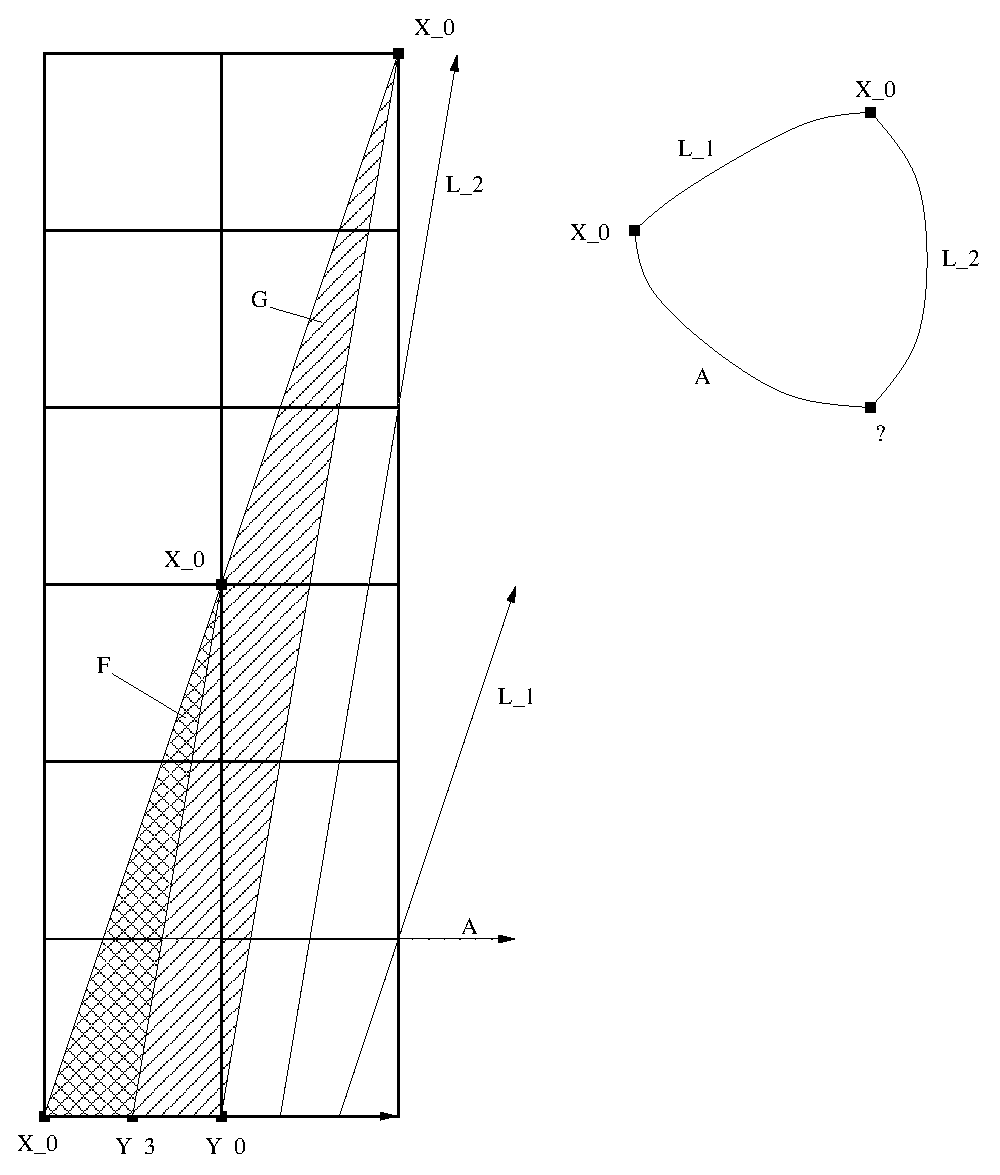
\includegraphics[width=0.45\textwidth]{figures/fig3.pdf}
  \caption{$u$ 平面上的奇点与单值变换。奇点位于 $u=-1,\,1,\,\infty$；绕 $u=-1$、$u=1$ 的回路分别给出
           单值矩阵 $M_{-1}$、$M_{1}$，绕无穷远的回路给出 $M_\infty=M_1M_{-1}$。原文仅标 “Figure 3”
           （原文 PDF 第 60 页），无说明性图注。}
  \label{fig:3}
\end{figure}

% [Tutor Note: 图 3（原文 PDF 第 60 页）与原文 PDF 第 59--60 页的丛语言。$u$ 平面去掉三个奇点后，
%  周期向量 $(a_D,a)^T$ 是平坦 $SL(2,{\rm Z})$ 丛 $V$ 的全纯截面；绕 $u=-1$、$u=1$、$u=\infty$ 的
%  回路分别给出 $M_{-1},M_1,M_\infty$，且按回路的复合次序 $M_\infty=M_1M_{-1}$（先绕 $u=-1$，
%  再绕 $u=1$，合成回路等效于绕无穷远）。把乘积次序写反会得到 $M_\infty^{-1}$。]

更确切地说，$(a_D(u), a(u))$ 构成丛 $V\otimes {\bf C}$ 的全纯截面，并具有如下渐近行为
\begin{eqnarray}
u\approx \infty\,:&\qquad& \left\{\, \begin{array}{l}
a \cong \sqrt{2u}\,  \\
a_D \approx i\;\frac{\sqrt{2u}}{\pi}\;{\rm ln}\; u
\end{array} \right. \,, \nonumber\\
u=1\,:&\qquad& \left\{\, \begin{array}{l}
a_D \approx \,c_0 (u-1) \\
a \approx a_0 + \frac{i}{\pi} \; a_{D}{\rm ln}\; a_{D}
\end{array} \right. \,.\nonumber
\end{eqnarray}
其中 $a_0$ 与 $c_0$ 为常数。对 $u=-1$，行为与 $u=1$ 类似，只需把 $a_D$ 换为 $a-a_D$。
模空间上的度规为 $ds^2={\rm Im}(\tau)\,|da|^2$，其中
\begin{equation}
\tau =\frac{da_D/du}{da / du}\,.
\label{tau-metric}
\end{equation}
为保证动能的正定性，${\rm Im}(\tau)$ 应当是正定的。这些单值变换生成子群 $\Gamma(2)$，它包含在 $SL(2,{\rm Z})$ 中；事实上，带奇点的 $u$ 平面就是上半平面 $H$ 对 $\Gamma(2)$ 的商。该商有三个尖点，
对应三个奇点。

% [Tutor Note: 原文 PDF 第 60 页未编号的渐近行为公式。弱耦合下 $u=\frac12a^2$（原文第 54 页），
%  故 $a\cong\sqrt{2u}$；而 $a_D\approx i\frac{\sqrt{2u}}{\pi}\ln u$ 中的 $i$ 与 $\pi$ 来自单圈预势
%  （见第 54 页 $\partial{\cal F}/\partial a$ 一式）。注意此式是对 $u$ 取对数，而不是对 $a$ 取对数，
%  二者相差 $\ln a^2=2\ln a$ 的常数项。在 $u=1$ 附近，$a_D\approx c_0(u-1)$ 是“磁单极无质量”的标志，
%  而 $a\approx a_0+\frac{i}{\pi}a_D\ln a_D$ 表明此时 $a_D$ 才是好坐标、$a$ 是坏坐标；$u=-1$ 处
%  作替换 $a_D\to a-a_D$。]

% [Tutor Note: 式 (\ref{tau-metric})（原文编号 (105)，原文 PDF 第 60 页）。$\tau=da_D/da$ 在 $u$
%  坐标下写成 $(da_D/du)/(da/du)$；弱耦合区 $\tau=\theta/2\pi+4\pi i/g^2$，故
%  ${\rm Im}\,\tau=4\pi/g^2>0$ 正是动能项正定。$S$ 对偶 $\tau\to-1/\tau$ 伴随
%  $(a_D,a)\to(a,-a_D)$ 的 $SL(2,{\rm Z})$ 作用，即“电—磁”互换；不要把 $a_D$ 与 $a$ 误当成纯虚、
%  纯实的量，它们一般是复的，只有 $\tau$ 的虚部才有正定意义（原文此处对“虚实变换”未加说明）。]

空间 $H/\Gamma(2)$（即 $u$ 平面）也参数化一族曲线 $E_u$，它们由方程
\begin{equation}
y^2 = (x-1)(x+1)(x-u)\,, 
\label{cubic}
\end{equation}
描述，其中 $x$ 是复变量。首先注意，该方程在变换
$$
w:\{u\rightarrow -u\,,x\rightarrow -x\,,y\rightarrow \pm iy \}\,,
$$
下不变；这些变换生成 ${\bf Z}_{4}$ 对称性，其中只有 ${\bf Z}_{2}$ 子群作用在 $u$ 上。
这与 ${\cal M}$ 上的对称性结构相同。现在来描述上述方程所代表的曲线。曲线基本上就是 $x$ 空间，
其拓扑由“$y$ 是单值函数”这一要求决定。由于方程对 $y$ 是二次的，若在 $x$ 空间沿绕 $y$ 的任意
一个零点的闭合回路走一圈，就有 $y\rightarrow -y$。对包含全部零点的回路也同样如此；等价地说，
绕 $x=\infty$ 的回路也如此（这是因为零点数为奇数）。因此，要使 $y$ 成为单值函数，$x$ 空间应当
是复平面 ${\bf C}$（再补上无穷远点）的双重覆叠。此外，该空间应在 $x=-1,1,u,\infty$ 处有四个
分支点，它们两两由两条割线相连（图 4）。为明确起见，取一条从 $-1$ 到 $1$ 的分支割线，另一条
从 $u$ 到 $\infty$。两张叶沿这些割线相接，使得穿过割线时从一张叶走到另一张叶。$y$ 正是在这个
空间上单值。

% [Tutor Note: 式 (\ref{cubic})（原文编号 (106)，原文 PDF 第 60 页）。验证 $\mathbf{Z}_4$：在
%  $u\to-u,\ x\to-x,\ y\to\pm iy$ 下，右端变为 $(-x-1)(-x+1)(-x+u)=-(x^2-1)(x-u)$，而左端
%  $(\pm iy)^2=-y^2$，故方程不变。其中 $u\to-u$ 与 $x\to-x$、$y\to\pm iy$ 合起来才构成
%  $\mathbf{Z}_4$，而只有 $u\to-u$ 这一 $\mathbf{Z}_2$ 子群作用在模空间上；曲线族 $E_u$ 本身
%  则具有更大的 $\mathbf{Z}_4$。]

\begin{figure}[htbp]
  \centering
  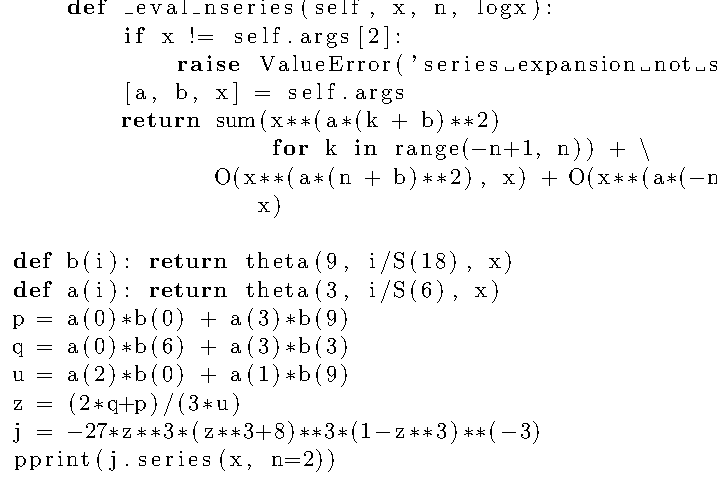
\includegraphics[width=0.60\textwidth]{figures/fig4.pdf}
  \caption{$x$ 空间：以 $x=-1,\,1,\,u,\,\infty$ 为分支点的双叶覆叠（亏格 1 的黎曼面）。两条割线分别连接
           $-1$ 与 $1$、$u$ 与 $\infty$；$a$-圈与 $b$-圈如图所示。原文仅标 “Figure 4”（原文 PDF 第 61 页），
           无说明性图注。}
  \label{fig:4}
\end{figure}

如此得到的 $x$ 空间正是一个亏格为 1 的黎曼面。这可以这样直观地看出：在环面上画一个圆 $c_1$，令其沿 $a$-圈环绕，再沿环面平移它得到圆 $c_2$（图 5(a)）。现在把圆 $c_1$ 与 $c_2$ 压扁成线段 $l_1$ 与 $l_2$
（图 5(b)）。这把环面分成沿这两条线段相接的两半。若把这两半都剪开，所得到的曲面就与上面描述的
$x$ 空间相同，其中 $l_1$ 与 $l_2$ 是两条分支割线，而无穷远点映为有限 $x$ 处的一点（图 5(c)）。

\begin{figure}[htbp]
  \centering
  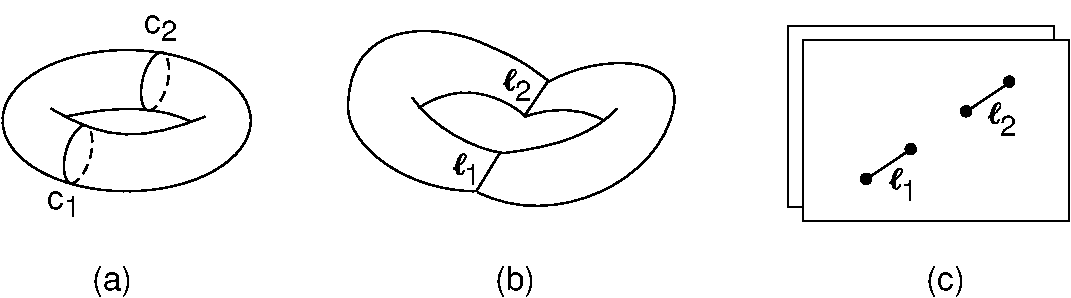
\includegraphics[width=0.95\textwidth]{figures/fig5.pdf}
  \caption{由环面理解 $x$ 空间。(a) 环面上的 $a$-圈 $c_1$ 与 $b$-圈 $c_2$；(b) 将 $c_1,c_2$ 压扁为线段
           $l_1,l_2$，环面被分成沿此二线段相接的两半；(c) 沿 $l_1,l_2$ 剪开两半后所得的双叶结构，即 $x$ 空间。
           原文仅标 “Figure 5”（原文 PDF 第 61 页），无说明性图注。}
  \label{fig:5}
\end{figure}

% [Tutor Note: 图 4、图 5（原文 PDF 第 61 页）。$y^2=(x-1)(x+1)(x-u)$ 对 $y$ 是二次的，故
%  $x$ 空间是 $\mathbf{C}\cup\{\infty\}$ 的双重覆叠，四个分支点 $-1,1,u,\infty$ 两两相连成两条割线；
%  割线的具体取法不唯一（这里取 $[-1,1]$ 与 $[u,\infty]$），不同取法只改变同调基的辛基底，不改变
%  物理。图 5 用环面说明：$c_1,c_2$ 压扁为 $l_1,l_2$ 后剪开，得到双叶结构；$x$ 平面上绕单条割线的
%  回路对应 $a$-圈，与两条割线都相交的回路对应 $b$-圈。]

由此清楚可见，$x$ 平面上绕两条割线之一走一圈的回路，对应环面的 $a$-圈；另一方面，与两条割线都
相交的回路（在我们的情形中，绕 $1$ 与 $u$），对应环面上的 $b$-圈。注意，当 $x$ 空间上两个分支点
重合时，曲线 $E_u$ 上的一个圈收缩为零，曲线变为奇异。例如在我们的情形中，若 $u=\infty$，
$a$-圈收缩为零；而 $u=1$ 时，这发生在 $b$-圈上。于是 $u$ 平面上的奇点正是族 $E_u$ 中某条曲线出现消失圈之处。

% [Tutor Note: 原文 PDF 第 62 页。奇点处消失圈与单值变换的对应是本节的核心：$u=\infty$ 时
%  $a$-圈收缩（对应 $M_\infty$），$u=1$ 时 $b$-圈收缩（对应 $M_1$）；由 $\mathbf{Z}_2$ 对称性
%  $u\to-u$，$u=-1$ 处同样是一个 $b$-圈收缩（对应 $M_{-1}$，但基底经 $a_D\to a-a_D$ 重排）。
%  这也解释了 $H/\Gamma(2)$ 为何恰有三个尖点——尖点即消失圈的位置。]

为确定 $a_D$ 与 $a$，在亏格为 1 的黎曼面 $E_u$ 上取两条独立的一维圈 $\gamma_1$ 与 $\gamma_2$，
并归一化使其相交数为 1：
$$
\gamma_1 \cdot \gamma_2 = 1\,.
$$
这些圈随 $u$ 连续变化，构成 $V_u=H^1(E_u,{\rm C})$ 这一 $E_u$ 的一阶同调群的局部基。一个圈可以与
一阶上同调群中的元素 $\lambda$ 配对：
$$
\gamma \rightarrow  \oint_{\gamma} \lambda\,.
$$
$\lambda$ 可看作亚纯 $(1,0)$-形式，定义在 $E_u$ 上，留数为零，模去恰当形式。留数为零保证该配对在
$\gamma$ 的连续形变下不变，即使形变越过 $\lambda$ 的极点。借助这一配对，我们也可把 $\lambda$
视为 $V_u$ 的元素。对 $E_u$ 上的 1-形式，可以取基底
$$
\lambda_{1} = \frac{dx}{y}\,, \qquad \lambda_{2} = \frac{xdx}{y}\,.
$$
不计标量倍数，$\lambda_1$ 是 $E_u$ 上唯一的全纯微分；若定义
$$
b_i=\oint_{\gamma_i}\lambda_1\,,\qquad{\rm for}\quad i = 1,2\,,
$$
则环面由参数
$$
\tau_u = b_1/b_2\,,\qquad {\rm with} \quad {\rm Im}(\tau_u) > 0\,. 
$$
刻画。考虑任意截面
$$
\lambda = a_1(u) \lambda_1 + a_2 (u) \lambda_2\,,
$$
（它是 $V_u$ 的截面），并暂时作如下等同：
$$
a_D=\oint_{\gamma_1}\lambda\,,\qquad a=\oint_{\gamma_2}\lambda\,.
$$
若 $\lambda$ 是留数为零的形式，则绕奇点一圈时 $a_D$ 与 $a$ 按正确的方式变换，这完全由
$\gamma_1$ 与 $\gamma_2$ 在 $SL(2,Z)$ 的某个子群下的变换决定（这一点在下面第 4.6 小节还会解释）。
另一方面，若 $\lambda$ 有一个留数非零的极点，则积分路径可能越过该极点，结果 $a_D$ 与 $a$ 可能
不再按纯粹的 $SL(2,Z)$ 变换。正如我们在前面某小节中已讨论的，在没有非零裸质量费米子的情形下，
这第二种可能性当然与 BPS 质量公式的对称性不一致。因此 $\lambda$ 不应有留数非零的极点（存在非零
裸质量费米子时情形不同，将在下一节末尾讨论）。上述对 $a_D$ 与 $a$ 的等同意味着
$$
\frac{da_D}{du}=\oint_{\gamma_1}\frac{d\lambda}{du}\,,\qquad
\frac{da}{du}=\oint_{\gamma_2}\frac{d\lambda}{du}\,.
$$
为固定 $\lambda$ 的任意性，我们利用条件 ${\rm Im}\tau > 0$，它正是 (\ref{tau-metric}) 所定义的
${\cal M}$ 上度规所要求的。首先设
$$
\frac{d\lambda}{du} = f(u) \lambda_{1} = f(u) \frac{dx}{y}\,.
$$
于是
$$
\frac{da_{D}}{du} = f(u)\,b_1\,,\qquad \frac{da}{du} = f(u)\,b_2\,,
$$
从而
$$
\tau = \frac{b_1}{b_2} = \tau_u\,. 
$$
由于 ${\rm Im}\,\tau_u > 0$，得到 ${\rm Im}\,\tau >0$。正如 Seiberg 与 Witten 所论证的，
逆命题也成立，因此 $d\lambda/du$ 不依赖于 $\lambda_2$。函数 $f(u)$ 由理论在 $u$ 平面奇点附近的
渐近行为固定，其值为 $f(u)=-\sqrt{2}/4\pi$。由此可得 $\lambda$ 为
$$
\lambda=\frac{\sqrt{2}}{2\pi}\;\frac{dx\sqrt{x-u}}{\sqrt{x^2-1}}=  
\frac{\sqrt{2}}{2\pi}\;\frac{dx y}{x^2-1}=\frac{\sqrt{2}}{2\pi}\;
\frac{dx}{y} (x-u) \,.
$$
为计算 $a$ 与 $a_D$，必须在 $E_u$ 上选取一组具体的一维圈基。我们把 $\gamma_2$ 等同于环面上的
$a$-圈，等价地，等同于一条绕点 $-1$ 与 $1$ 的曲线，这两个点取在 $x$ 平面上。可以把这条曲线形变到完全沿从 $-1$
到 $1$ 的割线来回。于是 $a(u)$ 由
\begin{equation}
a(u)=\frac{\sqrt{2}}{\pi}\,\int_{-1}^1\,\frac{dx\sqrt{x-u}}{\sqrt{x^2-1}}\,.
\label{au}
\end{equation}
给出。对 $\gamma_1$，取绕点 $1$ 与 $u$ 的曲线，得到
\begin{equation}
a_D(u)=\frac{\sqrt{2}}{\pi}\,\int_{1}^u\,\frac{dx\sqrt{x-u}}{\sqrt{x^2-1}}\,.
\label{adu}
\end{equation}
可以验证，在这样的圈选取下，$a$ 与 $a_D$ 在奇点附近具有所期望的行为 \cite{SW-I}。

% [Tutor Note: 原文 PDF 第 62 页。原文写 “first homology group $V_u=H^1(E_u,{\rm C})$”，严格说
%  $H^1$ 是上同调记号（同调应为 $H_1$）；因 $E_u$ 是紧致定向曲面，二者经 Poincaré 对偶同构，
%  后文按同调使用无碍，但引用时宜留意这一记号混用。留数为零的条件保证 $\oint_\gamma\lambda$
%  在 $\gamma$ 连续形变时不变（即使越过 $\lambda$ 的极点），这是 $\lambda$ 能作为 $V_u$ 元素并
%  与周期配对的前提。]

% [Tutor Note: 原文 PDF 第 63 页。由 $d\lambda/du=f(u)\,dx/y$ 与 $f(u)=-\sqrt2/4\pi$ 积分可得
%  $\lambda=\frac{\sqrt2}{2\pi}\frac{dx\sqrt{x-u}}{\sqrt{x^2-1}}$：因为
%  $\int du\,(x-u)^{-1/2}=-2\sqrt{x-u}$，负号与 $f$ 的负号相消，系数恰为 $\sqrt2/2\pi$。三个等号
%  用到 $y^2=(x^2-1)(x-u)$，即 $\frac{\sqrt{x-u}}{\sqrt{x^2-1}}=\frac{y}{x^2-1}=\frac{x-u}{y}$。
%  $\sqrt{x-u}$ 的分支约定与下面 $a_D$ 积分中出现的 $i$ 直接相关，不能随意选取。]

% [Tutor Note: 式 (\ref{au})、(\ref{adu})（原文编号 (107)、(108)，原文 PDF 第 63 页）。$\gamma_2$
%  沿 $[-1,1]$ 割线来回，故 $a(u)$ 的积分限为 $-1\to 1$；$\gamma_1$ 绕 $1$ 与 $u$，故积分限为
%  $1\to u$。两式的积分路径都取在相应割线的同一侧，上下限方向决定整体符号；若把 $\gamma_1$ 的
%  定向取反，$a_D$ 变号，继而 $M_1$、$M_{-1}$ 都会改变，务必与原文约定一致。原文在此引 \cite{SW-I}
%  验证了渐近行为。]

\noindent\underline{$a(u)$ 与 $a_D(u)$ 的显式表达式：}

容易求出 $a$ 与 $a_D$ 的显式表达式，其形式为完全椭圆积分 $E(k)$ 与 $K(k)$；所用的工具是
超几何函数 $F(\alpha,\beta,\gamma;z)$ 的积分表示 \cite{GR}。超几何函数由下式给出
\begin{eqnarray}
F(\alpha,\beta,\gamma;z)&=& \frac{\Gamma(\gamma)}{\Gamma(\beta)
\Gamma(\gamma-\beta)}\int_0^1\,dx\,x^{\beta-1} (1-x)^{\gamma-\beta-1}
(1-zx)^{-\alpha}\nonumber\\ 
&=& \frac{\Gamma(\gamma)}{\Gamma(\alpha)\Gamma(\beta)}\sum_{n\geq 0}
\frac{\Gamma(\alpha +n)\Gamma(\beta +n)}{\Gamma(\gamma +n)}\,
\frac{z^n}{n!}\,.\nonumber
\end{eqnarray}
将其与 (\ref{au}) 中 $a$ 的积分表示比较，容易看出
$$
a(u)=\sqrt{2(1+u)}\, F\left(-1/2, 1/2, 1; 2/(1+u)\right)\,.
$$
至于 $a_D$，先在 (\ref{adu}) 中作代换 $x=(u-1)t+1$。这给出
$$
a_D(u)=\frac{i}{\pi} (u-1)\int_0^1\,dt\,t^{-\frac{1}{2}}
(1-t)^{\frac{1}{2}} (1-\frac{1-u}{2} t)^{-\frac{1}{2}}\,. 
$$
将其与超几何函数的表达式比较，得到
$$
a_D(u)=\frac{i}{2} (u-1) F\left(1/2, 1/2, 2; (1-u)/2\right)\,.
$$

% [Tutor Note: 原文 PDF 第 64 页超几何函数的两种表示。积分表示前的 $\Gamma$ 因子是
%  $\Gamma(\gamma)/[\Gamma(\beta)\Gamma(\gamma-\beta)]$，而级数表示前是
%  $\Gamma(\gamma)/[\Gamma(\alpha)\Gamma(\beta)]$——两者并不相同，极易误抄成同一个；积分表示还要求
%  ${\rm Re}\,\gamma>{\rm Re}\,\beta>0$。另注意原文把 $F$ 的自变量写在分号之后
%  （$F(\alpha,\beta,\gamma;z)$），与某些文献的 $F(\alpha,\beta;\gamma;z)$ 记法只是标点差别。]

% [Tutor Note: 原文 PDF 第 64 页。在 $a_D$ 的积分 (\ref{adu}) 中作 $x=(u-1)t+1$，则
%  $x-u=(u-1)(t-1)$；在 $u>1$ 的割线一侧、$t\in[0,1]$ 上，
%  $\sqrt{x-u}=i\sqrt{u-1}\sqrt{1-t}$，同时
%  $\sqrt{x^2-1}=\sqrt{(u-1)t\,[(u-1)t+2]}$。整理后出现的 $i$、$(u-1)$ 以及
%  $(1-u)/2=-k'^2/k^2$ 中的负号，是这一段最易出错的地方，务必逐步核对。]

用超几何函数表示，完全椭圆积分为
\begin{eqnarray}
K(k) &=& \frac{\pi}{2}\, F\left(1/2, 1/2, 1; k^2\right)\,,\nonumber\\
E(k) &=& \frac{\pi}{2}\, F\left(-1/2, 1/2, 1; k^2\right)\,.\nonumber
\end{eqnarray}
进而定义 $k'^2=1-k^2$，并令
$$
E'(k)\equiv E(k')\,,\qquad K'(k) \equiv K(k')\,.
$$ 
现在利用恒等式
$$
c(1-z)F(a,b,c;z) - c F(a,b-1,c;z) + (c-a)z F(a,b,c+1;z)=0\,,
$$ 
取 $c=1, a=b=1/2$ 且 $z=(1-u)/2$，代入 $a_D$ 的表达式，得到
\begin{eqnarray}
a(u)   &=& \frac{4}{\pi k} E(k)\,,\nonumber\\
a_D(u) &=& \frac{4}{i\pi} E(i\frac{k'}{k}) + 
\frac{4i}{\pi k^2} K(i\frac{k'}{k})\,.\nonumber
\end{eqnarray}
这里 $k^2=2/(1+u)$，$(1-u)/2=-k'^2/k^2$。若注意到
$$
F(a, b, c; z)=(1-z)^{-a} F(a, c-b, c; z/(z-1))=
(1-z)^{-b} F(b, c-a, c; z/(z-1))\,.
$$
则这些表达式可以进一步简化。上式蕴含 $K(ik'/k)=kK(k')=kK'(k)$ 与
$E(ik'/k)=k^{-1}E(k')=k^{-1}E'(k)$，于是
\begin{eqnarray}
a(u)  &=& \frac{4}{\pi k}\, E(k)\,,\nonumber\\
a_D(u)&=& \frac{4}{\pi i}\,\frac{E'-K'}{k}\,.\nonumber
\end{eqnarray}
广义耦合 $\tau$ 可利用
\begin{eqnarray}
\frac{dE}{dk}&=&\frac{E-K}{k}\,,\quad 
\frac{dK}{dk}=\frac{1}{kk'^2}\,(E-k'^2 K)\,,\nonumber\\
\frac{dE'}{dk}&=&-\frac{k}{k'^2}\,(E'-K')\,,\quad 
\frac{dK'}{dk}=-\frac{1}{kk'^2}\,(E'-k^2 K')\,,\nonumber
\end{eqnarray}
算出，结果为
$$
\tau=\frac{\partial a_D}{\partial a}=\frac{da_D/dk}{da/dk}
=\frac{iK'}{K}\,.
$$

% [Tutor Note: 原文 PDF 第 64 页椭圆积分约定。这里 $K(k),E(k)$ 的宗量是模数 $k$，而不是参数
%  $m=k^2$：$K(k)=\frac{\pi}{2}F(1/2,1/2,1;k^2)$，$E(k)=\frac{\pi}{2}F(-1/2,1/2,1;k^2)$。原文只写
%  $E(k),K(k)$ 而未声明约定，引用文献数据时务必注意 $K(m)$ 与 $K(k)$ 相差一个 $k\to\sqrt m$
%  的代换；$k'^2=1-k^2$ 为补模。]

% [Tutor Note: 原文 PDF 第 65 页。$F(a,b,c;z)=(1-z)^{-a}F(a,c-b,c;z/(z-1))$ 是超几何函数的分式
%  线性变换，由此得 $K(ik'/k)=kK'(k)$、$E(ik'/k)=k^{-1}E'(k)$。注意 $|ik'/k|$ 一般不在 $[0,1)$
%  内，$K,E$ 需解析延拓；又 $E'$、$K'$ 是 $E(k')$、$K(k')$ 的简写，不是对 $k$ 的导数——原文的
%  撇号在这两节里有“补模”与“导数”两种含义，读到 $dE'/dk$ 时尤须分清。]

% [Tutor Note: 原文 PDF 第 65 页末。由 $a=\frac{4}{\pi k}E(k)$、
%  $a_D=\frac{4}{\pi i}\frac{E'-K'}{k}$ 对 $k$ 求导：
%  $\frac{da}{dk}=-\frac{4}{\pi}\frac{K}{k^2}$，
%  $\frac{da_D}{dk}=\frac{4}{\pi i}\frac{K'}{k^2}$（注意 $E'=E(k')$、$K'=K(k')$ 中 $k'^2=1-k^2$
%  也依赖 $k$，求导时不能漏掉 $dk'/dk=-k/k'$），二者相除才得 $\tau=iK'/K$。若漏掉补模对 $k$ 的
%  依赖，会得到相差一个 $k$ 因子的结果。]
   % §3.6--§3.9（原文 PDF 54--65 页）
%=====================================================================
%  分片 G：§4 含物质的 $N=2$ 规范理论的 Seiberg--Witten 分析
%  覆盖原文 PDF 第 65--80 页（§4 标题与导语、§4.1--§4.6，含图 6、图 7）
%=====================================================================

\section{含物质的 $N=2$ 规范理论的 Seiberg--Witten 分析}

\begin{keypoints}
\begin{itemize}
\item \textbf{物理图像：}加入 $N_f$ 个物质超多重态后，库仑分支上除磁单极/双子奇点外还出现夸克变无质量的奇点；奇点位置随裸质量移动，$m_i=0$ 时其数目与电荷由 $R$ 对称性的离散子群和中心荷的变换性质所决定。
\item \textbf{数学工具：}电荷归一化改为 $n_e\to2n_e$、$a\to a/2$，且 $2a_D=\partial{\cal F}/\partial a$；有物质时单值变换成为作用在 $(m/\sqrt2,a_D,a)^T$ 上的 $3\times3$ 矩阵（见原文 PDF 第 72 页），故对偶群一般不再是 $SL(2,Z)$，谱也仅在 $N_f=4$ 时才可能保持 $SL(2,Z)$ 不变。
\item \textbf{关键结论：}无质量各理论的 Seiberg--Witten 曲线为 $N_f=0$：$y^2=x^3-ux^2+\frac14\Lambda^4x$；$N_f=1$：$y^2=x^2(x-u)+t\Lambda_1^6$；$N_f=2$：$y^2=(x^2-\tilde\Lambda_2^4)(x-u)$；$N_f=3$：$y^2=x^2(x-u)+\tilde\Lambda_3^2(x-u)^2$。
\item \textbf{BPS 态：}零裸质量夸克（$SO(2N_f)$ 的矢量）与磁单极（$2N_f$ 个费米子零模生成 $Spin(2N_f)$ 的旋量）满足 $M=\sqrt2\,|Z|$，其中 $Z=n_ea+n_ma_D+S\,m/\sqrt2$；$N_f=1,3$ 时存在宇称简并，$N_f=2,4$ 时没有。
\item \textbf{几何对应：}模空间视为椭圆曲线族 $E_u$ 的模空间，$a,a_D$ 为其周期；判别式零点阶数给出单值变换的指数，$u\to\infty$ 处 $M_\infty=PT^{N_f-4}$，且有限奇点处单值矩阵之积应等于 $M_\infty$。
\end{itemize}
\end{keypoints}

本节我们考虑规范群为 $SU(2)$、并与 $N_f$ 个物质多重态耦合的 $N=2$
超对称规范理论。这一分析牵涉许多技术性问题，理论的性质依赖于 $N_f$
的取值。与通常的 QCD 一样，物质场（费米子）与规范玻色子对 $\beta$
函数的贡献符号相反。因此，为保证渐近自由，我们要求 $N_f
\leq 4$。$N_f =4$ 的理论在微扰论的各阶都是有限的，而且当夸克无质量时，
它极可能在非微扰层次上也是共形不变的。Seiberg 与 Witten
给出了证据，表明这一理论是 $SL(2,Z)$ 不变理论的一个例子。四维中已知的
另一个 $SL(2,Z)$ 不变理论是 $N=4$ 超对称规范理论，它的 $\beta$
函数同样为零。不过，下文我们将主要集中于 $N_f\leq 3$。至于 $N_f=4$
的情形，读者可参阅 Seiberg 与 Witten 的原始工作 \cite{SW2}。

% [Tutor Note: 见原文 PDF 第 65 页导语第一段。原文称“为保证渐近自由要求 $N_f\le4$”，
% 但由式 (111) 可见 $N_f=4$ 时 $\beta(g)=0$：该理论是有限的（共形不变），
% 并非渐近自由；严格的渐近自由条件是 $N_f<4$。此处是原文的宽泛表述，阅读时不要
% 把 $N_f=4$ 当作渐近自由理论。]

有物质存在时，采用一个不同于前几节的电荷归一化会比较方便。在 $N=2$
纯规范理论中，所有场都按伴随表示变换，粒子与磁单极的荷都是整数。因此，
在公式 $Z=a n_e + a_D n_m$ 中，$n_e$ 与 $n_m$ 都是整数。按这一归一化，
一旦引入夸克，$n_e$ 就可能取半整数。本节我们采用一个稍有不同的约定：
为保证 $n_e$ 始终为整数，把它乘以 2，同时把 $a$ 除以 2，以保持质量公式
不变。由于 $a_D$ 保持不变，它现在由 $2 a_D=\partial{\cal F}/\partial a$
给出。用规范不变量 $u={\rm Tr}\phi^2$ 表示，当 $|u|\rightarrow\infty$ 时，
在这一归一化下 $a$ 与 $a_D$ 的渐近行为变为
$$
a \cong \frac{1}{2} \sqrt{2u}\,, \quad
a_D \simeq i \frac{4}{\pi} a \log a\,.
$$

% [Tutor Note: 见原文 PDF 第 65 页。与第 3 节的纯规范归一化对照：那里
% $a\cong\sqrt{2u}$、基本表示的夸克 $n_e=\pm1/2$、$W$ 玻色子 $n_e=\pm1$；
% 本节把 $n_e$ 乘 2、$a$ 除 2，于是 $a\cong\frac12\sqrt{2u}$ 而 $a_D$ 不变
% （$2a_D=\partial{\cal F}/\partial a$）。这个因子 2 贯穿全节，尤其是式
% (113)、第 76 页的换基与式 (115)，核对时最易出错。]

此外，有效耦合也被重新标度为 $\tau=\partial a_D/\partial a = \frac{\theta}{\pi}
+ \frac{8 \pi i}{g^2}$。电荷的这一重新标度会改变确定模型解的曲线形式，
但物理保持不变。

本节我们将研究规范群为 $SU(2)$ 的理论。在这种情况下，最有趣的动力学
出现在模空间的库仑分支上，在那里 $SU(2)$ 破缺为 $U(1)$。因此，先研究
$N = 2$ 超对称 QED 是有启发性的。

\subsection{$N = 2$ 超对称量子电动力学（SQED）}

$N=2$ 超对称 QED 包含光子矢量多重态与 $k$ 个夸克超多重态。光子多重态
由 $N=1$ 手征超场 $(W_{\alpha}, A)$ 组成，每个夸克超多重态由两个 $N=1$
手征超场 $M^i$ 与 $\widetilde M_i$ 组成，它们的 $U(1)$ 荷分别为 $+1$ 与
$-1$。唯一可重整且与 $N = 2$ 相容的超势是：
$$
{\cal W}=\sqrt{2} A M^i\widetilde M_i + \sum_i m_i M^i\widetilde
M_i\,. 
$$

% [Tutor Note: 见原文 PDF 第 66 页。$A$ 是光子矢量多重态的 $N=1$ 手征超场
% （其最低分量为复标量），$W_\alpha$ 是场强手征超场；$M^i$ 与 $\widetilde M_i$
% 的味指标 $i$ 与 $U(1)$ 规范指标都隐含缩并。超势中的 $\sqrt2$ 系数不是可以
% 随意改动的约定：它保证同一超多重态内玻色子与费米子质量简并，并与 BPS 质量
% 公式中的 $\sqrt2$ 相关联。]

当 $m_i = 0$ 时，理论具有整体对称群 $SU(k)\times SU(2)_R \times
U(1)_{\cal R}$。$SU(k)$ 是作用于 $k$ 个超多重态的味对称群，$SU(2)_R$
转动两个超对称，而 $U(1)_{\cal R}$ 是通常的 $R$ 对称性，它受反常的破坏。
与无物质的情形一样，策略是先确定经典模空间，再看量子模空间是否定性不同。
理论的对称性对于确定这些模空间的结构非常有用。

% [Tutor Note: 见原文 PDF 第 66 页。原文 “afflicted by an anomaly” 一语指该整体
% 对称性被瞬子反常破缺（下一小节将具体算出 ${\bf Z}_{4N_c-2N_f}$），并非说它
% 完全不是对称性；故译作“受反常的破坏”，而非“具有反常”。]

一般而言，经典模空间有希格斯分支与库仑分支。希格斯分支由某些 $M^i$
获得真空期望值来定义。在这种情况下，无论在 QED 中还是在规范群为 $SU(2)$
的 QCD 中，规范群都被完全破缺。对 $k=1$，不存在希格斯相。当 $k \geq 2$、
$m_i = 0$ 时，利用整体对称性以及 $D$ 项的消失条件，可以把 $M$ 与
$\widetilde M$ 转到 $M=(B,0,0,...)$ 与 $\widetilde M = (0,
B,0,...)$ 的形式。由此可以读出依赖于味数 $k$ 的各种对称性破缺模式。
处在希格斯分支上的理论不含磁单极或双子，因此其动力学可能性不如库仑分支
丰富。经典模空间是一个超凯勒流形，理论的对称性在其上导致唯一的超凯勒
度规。由于这一唯一性，该度规没有量子修正。因此，在希格斯分支上，
经典模空间与量子模空间相同。

在现在的情形下，若所有 $m_i = 0$，则库仑分支由 $<A> \not= 0$ 定义，
而这又意味着 $<M^i>=<\widetilde M_i>=0$。$U(1)$ 规范群保持未破缺，
而所有 $M$ 都获得质量。在模空间的一般点上，有效低能理论（只涉及无质量
模）是一个纯 $N=2$ 规范理论，凯勒势属于特殊几何型：$K={\rm Im} a_D (a)
\bar{a}$。通过 $N=2$ 超对称，它与规范动能项相联系，
$$
\int d^2 \theta \; \frac{\partial a_D}{\partial a} \;
W^{\alpha}W_{\alpha}\,.
$$

凯勒势（因而度规）会获得量子修正，但 $K$ 的单圈近似是精确的，而且没有
非微扰修正，因为该理论不含瞬子。利用含 $k$ 个超多重态的 QED 的单圈
$\beta$ 函数，我们得到
\begin{equation}
a_D = - \frac{ik}{2\pi} \; a \ln (a/\Lambda)\,.
\label{beta-hyper}
\end{equation}
要重现这个公式，需注意超对称地定义 $g$ 的方式中额外的因子 $2$，以及前面
提到的归一化约定。由此得到的度规 ${\rm Im}
(\tau)$ 在 $|a| = \Lambda / e$ 处为零，因而有效耦合常数是奇异的。由于这一
朗道极点奇点，理论在紫外区域没有意义，除非它被嵌入到一个渐近自由的更大
理论中。若加入费米子质量项，库仑分支上的奇点就可以移动。因为当 $a = -
\frac{1}{\sqrt{2}} m_i$ 时一个电子变为无质量，我们有
$$
a_D = - \frac{i}{2\pi} \sum_i (a+m_i / \sqrt{2}) \;\ln
\frac{(a+m_i / \sqrt{2})}{\Lambda}\,.
$$
现在每个裸质量都对应模空间上的一个奇点，在那里该粒子变为无质量。取决于
两个或更多质量是否可能相等，可以出现希格斯分支与库仑分支相接触的情形，
从而导致复杂的结构。

% [Tutor Note: 见原文 PDF 第 67 页式 (109)。QED 的 $U(1)$
% $\beta$ 函数为正（红外自由），故 $a_D$ 的系数是 $-ik/2\pi$，与纯 $N=2$
% 理论大 $u$ 处的 $+i(4-N_f)/2\pi$（式 (113)）反号；此处极易
% 漏掉负号。另注意该式是对 $k$ 个电子求和前的单圈结果，$\ln(a/\Lambda)$ 的
% 宗量是 $a$（量纲 1），与式 (113) 中的 $u/\Lambda^2_{N_f}$ 不同。
% 由 $\tau=\partial a_D/\partial a$ 可核验 ${\rm Im}\,\tau=0$ 恰好发生在
% $|a|=\Lambda/e$，即朗道极点。]

这里我们也看到第 2 节讨论过的 $N = 2$ 代数中心荷修正形式的一种体现。
对纯 $N=2$，我们有 $Z = n_e a + n_m a_D$。然而现在电子的质量并不只是
$\sqrt{2} |a|$，而是第 $i$ 个多重态具有质量
$|\sqrt{2} a + m_i |$。正如第 2 节所示，这与下述事实一致：有质量超多重态的
$U(1)$ 荷 $S_i$ 出现在中心荷 $Z$ 的公式中，即
$$
Z = n_e a + n_m a_D + \sum_i S_i m_i / \sqrt{2}\,.
$$

% [Tutor Note: 见原文 PDF 第 67 页末。中心荷多出 $\sum_iS_im_i/\sqrt2$ 项，
% 故 BPS 质量 $M=\sqrt2|Z|$ 给出 $|\sqrt2a+m_i|$，而不是 $\sqrt2|a|$；
% 核对时注意 $m_i$ 前的 $1/\sqrt2$ 与 $a$ 前的 $\sqrt2$ 来自同一归一化，
% 不可对调。后文式 (84)（原书第 84 式）即此修改后的质量公式。]

\subsection{含物质的 $N=2$ 超对称量子色动力学（SQCD）}

与 $N_f$ 个物质超多重态耦合的 $N=2$ 超对称 QCD 包含 $N=1$ 超势
$$
W=\sum_{i=1}^{N_f}(\sqrt{2}\widetilde{Q}_i\Phi
Q^i+m_i\tilde{Q}_iQ^i)\,. 
$$
一般而言，当 $m_i=0$ 时，该理论具有整体对称群
$SU(N_f)\times SU(2)_R\times U(1)_{\cal R}$。在规范群为 $SU(2)$ 的特殊
情形下，味群扩大为 $O(2N_f)$。这是因为对 $SU(2)$ 而言，基本表示与其
复共轭表示同构，因此 $Q^i$ 与 $\widetilde Q_i$ 可以组合成一个按
$O(2N_f)$ 变换的 $2N_f$ 维矢量。于是，对 $SU(2)$ 规范群这一特殊情形，
理论还具有一个宇称对称群 ${\bf Z}_2\subset O(2N_f)$，其作用为
\begin{equation}
\rho : Q_1 \leftrightarrow \widetilde{Q}_1\,,
\label{rho}
\end{equation}
而其他所有场保持不变。这一宇称在理论分析中起着重要作用。理论的整体对称群
实际上是 $O(2N_f) \times SU(2)_R \times U(1)_{\cal R}$ 的一个商群。之所以
要取商，是因为 $Z_2 \subset U(1)_{\cal R}$ 与洛伦兹群中的 $(-1)^F$ 相同；
这个 $Z_2$ 与 $SU(2)_R$ 的中心相结合，恰好就是 $O(2N_f)$ 中心的
${\bf Z}_2$。

% [Tutor Note: 见原文 PDF 第 67--68 页。$SU(2)$ 中基本表示与共轭表示同构，
% $Q^i$ 与 $\widetilde Q_i$ 才能拼成 $O(2N_f)$ 的 $2N_f$ 维矢量；对
% $SU(N_c)$（$N_c>2$）这一步不成立，故 $N_c=2$ 的味对称性比一般情形大。
% 关于商群：$U(1)_{\cal R}$ 中心的 $Z_2$、$SU(2)_R$ 中心的 ${\bf Z}_2$ 与
% $O(2N_f)$ 中心的 ${\bf Z}_2$ 是同一个 ${\bf Z}_2$ 的不同化身，故整体
% 对称群要按对角线 ${\bf Z}_2$ 取商，否则会重复计数。]

对 $N_f = 0,1$，理论只有库仑分支，即 $(<\phi>
\not= 0)$。在这一分支上 $SU(2)$ 破缺为 $U(1)$，所有夸克都有质量。此外，
$U(1)_{\cal R}$ 自发破缺，因为 $\Phi$ 的 $U(1)_{\cal R}$ 荷为 $2$。
对 $N_f \geq 2$，我们可以有库仑分支，也可以有希格斯分支。在希格斯分支上，
规范对称性完全破缺，动力学并不丰富。我们将不详尽分析这一分支，只指出：
与 QED 情形一样，模空间上的度规由对称性唯一确定，且没有量子修正。

\noindent\underline{量子理论的一些性质}：
我们理论的微扰 $\beta$ 函数（由于超对称，它只是单圈效应）由下式给出
\begin{equation}
\beta (g) = - \frac{4-N_f}{16\pi^2} g^3.
\label{betanf}
\end{equation}
因此，为保证渐近自由，我们只考虑 $N_f=0,1,2,3,4$。

% [Tutor Note: 见原文 PDF 第 68 页式 (111)。负号对应 $N_f<4$ 的
% 渐近自由；$N_f=4$ 时 $\beta=0$，理论有限而非渐近自由（见本节导语的批注）。
% 若改用 $\alpha=g^2/4\pi$，渐近自由条件同样是 $4-N_f>0$。系数 $1/16\pi^2$
% 与 $g$ 的归一化有关，比较不同文献时先核对其 $\beta$ 函数定义。]

在上一节，通过数瞬子背景中的费米子零模，我们发现 $U(1)_{\cal R}$ 破缺为
离散子群 ${\bf Z}_{4N_c-2N_f}$。这是要求由
(\ref{G}) 给出的关联函数 $G$ 在 $U(1)_{\cal R}$ 下保持不变而得到的。
对 $N_c=2$，我们还有一个额外的离散对称群 (\ref{rho})，它置换费米子
零模 $\psi_{q_1}$ 与 $\widetilde\psi_{q_1}$。这个群是反常的，因为它把
$G$ 变为 $-G$。因此，现在我们可以允许那些不保持 $G$ 不变、而是把它改变
一个符号的 $U(1)_{\cal R}$ 变换。这个符号可以由一个反常的 ${\bf Z}_2$
变换来补偿。于是，对 $N_c=2$，$U(1)_{\cal R}$ 破缺为离散子群 ${\bf
Z}_{2(4N_c-2N_f)}={\bf Z}_{4(4-N_f)}$。它可以与反常的 ${\bf Z}_2$
结合，得到一个无反常的离散子群 ${\bf Z}_{4(4-N_f)}$，其作用为（见
(\ref{Rb1}) 与 (\ref{Rb2})）：
$$
\begin{array}{l}
\left.\begin{array}{l}
W_{\alpha} \rightarrow \omega W_{\alpha} (\omega^{-1} \theta )\\
\Phi \rightarrow \omega^2 \Phi (\omega^{-1} \theta )\\
Q^1  \rightarrow \widetilde Q_1 (\omega^{-1} \theta )\\
\widetilde Q_1  \rightarrow Q^1 (\omega^{-1} \theta ) \\
\end{array}\right. \\
\left.\begin{array}{l}
Q^i  \rightarrow Q^i (\omega^{-1} \theta )\\
\widetilde Q_i  \rightarrow \widetilde Q_i (\omega^{-1} \theta )\\
\end{array}\right\} \qquad i\not= 1\,,
\end{array}
$$
其中 $\omega={\exp}(2i\pi/4(4-N_f))$。对 $N_f = 0$，我们没有夸克来抵消
反常，只有上述变换的平方是无反常的。这一情形已在上一节讨论过。此外，
可以看出子群 ${\bf Z}_2 \subset {\bf Z}_{4(4-N_f)}$ 与洛伦兹群中的
$(-1)^F$ 相同。把上述变换与 $SU(2)_R$ 的 $U(1)_J$ 子群相结合（见
(\ref{Rb1}) 与 (\ref{Rb2})），我们得到一个与 $N=1$ 超对称对易的
${\bf Z}_{4(4-N_f)}$ 对称性
\begin{equation}
\begin{array}{l}
\left.\begin{array}{l}
\Phi \rightarrow \omega^2 \Phi(\theta) \\
Q^1 \rightarrow \omega^{-1} \widetilde{Q}_1(\theta) \\
\widetilde{Q}_1 \rightarrow \omega^{-1} Q^1(\theta) \\
\end{array} \right.\\
\left.\begin{array}{l}
Q^i \rightarrow \omega^{-1} Q^i(\theta) \\
\widetilde{Q}_1 \rightarrow \omega^{-1} \widetilde{Q}_i(\theta) 
\end{array} \right\}
\qquad i \not= 1\,.
\end{array}
\label{symm-A}
\end{equation}

% [Tutor Note: 见原文 PDF 第 68--69 页。$N_c=2$ 时
% ${\bf Z}_{2(4N_c-2N_f)}={\bf Z}_{2(8-2N_f)}={\bf Z}_{16-4N_f}
% ={\bf Z}_{4(4-N_f)}$，指数中 $4N_c-2N_f=8-2N_f$ 与后文 $4(4-N_f)$
% 只有在 $N_c=2$ 时才一致，代值核对时勿混用。$N_f=0$ 时没有夸克抵消反常，
% 只有变换的平方无反常，这与第 3 节的讨论一致。]

% [Tutor Note: 见原文 PDF 第 69 页。$\omega={\exp}(2i\pi/4(4-N_f))$ 应理解为
% $\omega=e^{2\pi i/[4(4-N_f)]}$，即 ${\bf Z}_{4(4-N_f)}$ 的本原根；原文排版
% “$2i\pi/4(4-N_f)$” 极易被误读成 $(2\pi i/4)(4-N_f)$。可用下一段的结果反验：
% $u$ 的荷为 4，故 $\omega^4=e^{2\pi i/(4-N_f)}$，恰给出
% $u\to e^{2\pi i/(4-N_f)}u$。]

% [Tutor Note: 原文 PDF 第 69 页式 (112) 第二组第二行左端写作
% $\widetilde{Q}_1$，据上下文（该组对 $i\ne1$ 的场统一乘 $\omega^{-1}$，
% 且与第一组的 $Q^1\leftrightarrow\widetilde Q_1$ 置换相区别）应为
% $\widetilde{Q}_i$。这是原文的排印笔误，公式按原样保留，阅读时请自行修正。]

在这一变换下，规范不变序参量 $u={\rm
Tr}\phi^2$ 的荷为 $4$，并按 $u \rightarrow \exp 2 \pi
i /(4-N_f) u$ 变换。这进一步把 ${\bf Z}_{4(4-N_f)}$ 破缺为 ${\bf
Z}_4$。剩余的 ${\bf Z}_{4-N_f}$ 在 $u$ 平面上非平凡地作用。注意对
$N_f=0$，不保持 $u$ 不变的子群只是一个 ${\bf Z}_2$。

与 $N_f = 0$ 情形一样，$a_D(u)$ 的大 $u$ 行为由单圈 $\beta$ 函数
(\ref{betanf}) 决定：
\begin{eqnarray}
a &\cong& \frac{1}{2} \sqrt{2u} + \cdots \,,\nonumber\\
a_D &\simeq& i \;\frac{4-N_f}{2\pi}\,a(u)\ln\frac{u}{\Lambda^2_{N_f}}
+ \cdots \,.\label{betanf-mon}
\end{eqnarray}
这里，省略号代表非微扰的瞬子修正。这些修正的一般形式可以通过与上一节
$N_f=0$ 情形类似的论证得到。首先，来自 $k$ 瞬子位形的修正正比于
$k$ 瞬子因子；利用 $\beta$ 函数 (\ref{betanf})，它可以写成
\begin{equation}
e^{-8\pi^2k/g^2} =\left(\frac{\Lambda_{N_f}}{a}\right)^{k(4-N_f)}\,. 
\label{inst-nf}
\end{equation}
遵循 Seiberg \cite{Seiberg-n,Seiberg-poh} 的做法，我们可以通过给 $u$
与 $\Lambda_{N_f}$ 赋予适当的荷，来恢复 $U(1)_{\cal R} \times {\bf Z}_2
(\rho )$ 对称性中破缺的部分。于是我们给 $u$ 赋荷 $4$、赋偶的
$\rho$-宇称，而给 $\Lambda_{N_f}^{4-N_f}$ 赋荷 $2 (4-N_f)$、赋奇的
$\rho$-宇称。注意在这一赋值下，单瞬子因子 $\exp(-8\pi^2/g^2)$ 具有奇的
$\rho$-宇称，它恰好补偿 (\ref{G}) 中关联函数 $G$ 在 ${\bf Z}_2(\rho)$
下的奇宇称，从而使之保持不变。对 $N_f=4$ 的特殊情形，$U(1)_{\cal R}$
无反常，$u$ 的荷为 $4$。$O(8)$ 中的 $Z_2(\rho)$ 仍是反常的，但同样可以
通过给瞬子因子 $\exp(-8\pi^2/g^2)$ 赋奇宇称而把它视为未破缺。在上述荷
赋值下要求 $U(1)_{\cal R}$ 不变，意味着每个修正项都应含有因子 $\sqrt u$。
此外，由于 $u$ 平面上的度规在 $\rho$-宇称下不变，具有奇瞬子数的位形不能
对 $a$ 与 $a_D$ 有贡献。把这些事实合在一起，我们可以把修正后的 $a$ 与
$a_D$ 的一般形式写成
\begin{eqnarray}
a &=& \frac{1}{2} \sqrt{2u} \left ( 1 + \sum_{n=1}^\infty a_n (N_f)
\left(\frac{\Lambda^2_{N_f}}{u}\right)^{n(4-N_f)} \right )\,,
\nonumber\\
a_D &=& i \frac{4-N_f}{2 \pi} a(u) \ln \frac{u}{\Lambda^2_{N_f}} +
\sqrt{u} \sum_{n=0}^\infty  a_{Dn} (N_f) \left(\frac{\Lambda^2_{N_f}}
{u}\right)^{n(4-N_f)} \,.\nonumber
\end{eqnarray}
计算系数 $a_n$ 与 $a_{Dn}$ 是困难的部分。

% [Tutor Note: 见原文 PDF 第 69 页。$a$ 的展开从 $n=1$ 开始，而 $a_D$ 的
% 展开从 $n=0$ 开始（$n=0$ 项是 $\sqrt u\,a_{D0}(N_f)$，即解析的非微扰修正）；
% 两式的幂次都是 $(\Lambda^2_{N_f}/u)^{n(4-N_f)}$，其中 $\Lambda^2_{N_f}$ 与
% $u$ 同量纲。注意 $a_D$ 对数项系数 $i(4-N_f)/(2\pi)$ 与 $a$ 的领头项
% $\frac12\sqrt{2u}$ 的 $N_f$ 依赖不同，且因子 $\sqrt u$ 整体提到求和号外，
% 抄写时最易漏掉。]

% [Tutor Note: 见原文 PDF 第 69 页。把 $\Lambda_{N_f}^{4-N_f}$ 的
% $U(1)_{\cal R}$ 荷定为 $2(4-N_f)$、$\rho$ 宇称为奇，这一赋值在 $N_f=4$ 时
% 退化为 $\Lambda^0$ 而失去意义；所以原文随后把 $N_f=4$ 单独处理。也因此，
% $N_f=4$ 的曲线不能由上述 $a,a_D$ 展开式直接取极限得到（参见原文第 79--80 页
% 与 [32]）。]

由于规范群 $SU(2)$ 破缺为 $U(1)$，理论将具有有质量的带电态，而我们想知道
未破缺的整体对称性如何作用于它们。整体对称性中未破缺的部分（即保持 $u$
不变的部分）可以通过把变换 (\ref{symm-A}) 取 $4-N_f$ 次幂得到。这一未破缺
变换改变 $\phi$ 的符号，因此对带电场的作用相当于电荷共轭。对 $N_f=1,3$；
$4-N_f$ 为奇数，未破缺变换含有 $\rho$ 的奇次幂。因此它在 $O(2N_f)$ 中
起宇称的作用。所以在这种情况下，宇称 (\ref{rho}) 在谱上得到实现，只是它
反转电荷与磁荷的符号。给定电荷的态属于 $SO(2)$（对 $N_f=1$）或 $SO(6)$
（对 $N_f=3$）多重态。对 $N_f=2,4$；$4-N_f$ 为偶数，未破缺变换只含
$\rho$ 的偶次幂。所有相当于宇称变换的 $\rho$ 奇次幂都属于破缺的变换。
因此在这种情况下，宇称对称性破缺，态只处于 $SO(4)$（对 $N_f=2$）或
$SO(8)$（对 $N_f=4$）表示中。

\subsection{BPS 饱和态}

在希格斯分支上 $SU(2)$ 完全破缺，不存在电荷或磁荷。因此 $N=2$ 代数的
中心荷只含超多重态 $U(1)$ 荷的贡献。我们将不详尽讨论这一点。

在库仑分支上，最简单的 BPS 饱和态是裸质量为零、并在规范对称性自发破缺
后获得质量 $M = \sqrt{2} |a|$ 的夸克。它们构成一组按 $SO(2N_f)$ 的
矢量变换的 BPS 态。除此之外，还有按 $SO(2N_f)$ 的旋量变换的 BPS 态，
其来源如下：由于规范对称性破缺为 $U(1)$，理论含有磁单极。在磁单极存在
时，每个费米子的 $SU(2)$ 二重态有一个零模。由于有 $N_f$ 个超多重态，
就有 $2N_f$ 个费米子二重态，因而有 $2N_f$ 个费米子零模。量子化后，这些
零模给出一个 $2N_f$ 维狄拉克代数，它提供 $SO(2N_f)$ 的旋量表示。于是
费米子零模把磁单极变成 $SO(2N_f)$ 的旋量。这与超弦理论中 Ramond 扇区的
量子化非常相似。旋量的存在表明，在量子层次上对称群是 $SO(2N_f)$ 的通用
覆盖，即 $Spin(2N_f)$。

% [Tutor Note: 见原文 PDF 第 70 页。要点是“$N_f$ 个超多重态 $\Rightarrow$
% $2N_f$ 个费米子二重态 $\Rightarrow$ 每个二重态在磁单极背景中各贡献一个
% 零模 $\Rightarrow$ 共 $2N_f$ 个零模 $\Rightarrow$ $2N_f$ 维 Clifford/Dirac
% 代数 $\Rightarrow$ $Spin(2N_f)$ 的旋量”。原文用“each $SU(2)$ doublet of
% fermions has one zero-mode”一句带过零模个数的计算（指标定理的结论），
% 具体可参看第 2、3 节关于零模的讨论。]

磁单极的集体坐标之一是电荷转动。量子化后，它导致磁单极具有一列带电荷的
态。然而，由电荷算符作 $2\pi$ 转动并不是恒等变换。利用 Witten 效应，这种
转动给出一个拓扑非平凡的规范变换，对 $n_m = 1$ 的磁单极，其本征值为
$e^{i \theta} (-1)^H$。这里 $(-1)^H$ 是 $SU(2)$ 的中心，对超多重态中的
态为奇，对矢量多重态中的态为偶。本节我们把电荷算符归一化，使基本夸克的荷
为 $\pm 1$、有质量规范玻色子的荷为 $\pm 2$。在这一归一化下，上述规范转动
可以写成算符等式
$$
e^{i \pi Q} = e^{i \theta n_m} (-1)^H.
$$
其中 $Q = n_e + n_m \theta/\pi$。由于 $n_e \in {\bf Z}$，这一关系意味着
$n_e$ 为偶数的态有 $(-1)^H = 1$，$n_e$ 为奇数的态有 $(-1)^H = -1$。
因子 $(-1)^H$ 可以等同于 $SO(2N_f)$ 旋量表示的手征算符。对 $N_f = 1,3$，
$SO(2N_f)$ 宇称变换作用于谱，它保证一个按 $SO(2N_f)$ 正手征旋量变换的
双子与一个具有相反电荷与磁荷、相反 $SO(2N_f)$ 手征的粒子简并。对
$N_f = 2,4$，不存在这种关系。

% [Tutor Note: 见原文 PDF 第 70 页。$e^{i\pi Q}=e^{i\theta n_m}(-1)^H$ 中
% “$2\pi$ 转动不是恒等变换”来自 Witten 效应：绕磁单极一周的电荷转动同时
% 产生一个 $\theta$ 角的规范变换。$(-1)^H$ 就是 $SU(2)$ 的中心元，
% 等价于 $Spin(2N_f)$ 旋量表示的手征算符，故 $n_e$ 的奇偶性与 $SO(2N_f)$
% 手征性相关联。核对时注意 $n_e$ 的符号约定（本节已把 $n_e$ 乘 2，
% 基本夸克 $n_e=\pm1$，见第 65 页）。]

对 $N_f > 0$，我们将看到谱中含有 $n_m > 1$ 的态。标记这些态的一个方便
方式是看它们在 $Spin(2N_f)$ 中心下的行为。
\begin{itemize}
\item

$N_f = 2$：\, $Spin(4) = SU(2) \times SU(2)$，中心为 ${\bf Z}_2
\times {\bf Z}_2$。中心的表示可以用 $(\epsilon , \epsilon ')$ 标记，
其中 $\epsilon = 0$ 对应类矢量的不可约表示，$\epsilon = 1$ 对应类旋量的
不可约表示。基本夸克按 $(\epsilon , \epsilon ') = (1,1)$ 变换。多夸克态
则按 $(n_e \; mod \; 2, n_e \; mod \; 2)$ 变换。由于磁单极的行为像旋量，
我们有
$$
(\epsilon , \epsilon ') = ((n_e + n_m) \; mod \; 2, n_e \; mod \; 2)
\qquad {\rm for}\,\, {N_f = 2}\,.
$$
\item
$N_f = 3$：\, $Spin(6) = SU(4)$，中心为 ${\bf Z}_{4}$。基本夸克处于
$Spin (6)$ 的 $6$ 中，因此它们相对中心的荷为 $2$。由于磁单极的行为像
旋量，我们得出结论：${\bf Z}_{4}$ 的作用为
$$
\exp \; \frac{i \pi}{4} (n_m + 2n_e)
\qquad{\rm for} \,\,{N_f = 3}\,.
$$
\item
$N_f=4$：\, $Spin(8)$ 的中心为 ${\bf Z}_2\times {\bf Z}_2$。因此，用与
上面类似的论证，我们得到

$(\epsilon,\epsilon')$$=$$(n_m\; mod\; 2, n_e\; mod \; 2) $。中心的四个
表示可以用实现它们的 $Spin(8)$ 表示来标记：$(0,1)\equiv v$，
$(1,0)\equiv s$，$(1,1)\equiv c$，$(0,0)\equiv o$。这里 $v$ 指矢量表示，
$s$ 与 $c$ 指两个旋量表示，$o$ 指平凡表示。$Spin(8)$ 有一个由外自同构
构成的三元性（triality）群，它同构于作用在 $v$、$s$、$c$ 上的置换群
${\bf S}_3$。
\end{itemize}

% [Tutor Note: 见原文 PDF 第 71 页。三条记号极易混淆：$N_f=2$ 时中心为
% ${\bf Z}_2\times{\bf Z}_2$，夸克的荷为 $(1,1)$，磁单极贡献使第一个
% ${\bf Z}_2$ 指标变为 $(n_e+n_m)\bmod2$；$N_f=3$ 时 $Spin(6)=SU(4)$ 的
% 中心是 ${\bf Z}_4$，基本夸克在 $6$ 中、相对中心的荷为 2，故相位是
% $e^{i\pi(n_m+2n_e)/4}$；$N_f=4$ 时 $Spin(8)$ 的中心两个 ${\bf Z}_2$
% 分别给出 $n_m$、$n_e$ 的奇偶。原文在 $N_f=4$ 处写“representatios”
% （应为 representations），系排印笔误。]

若打开一个 $N = 2$ 不变的质量，比如 $m_{N_f} \not= 0$，则
$SO(2N_f)$ 明显破缺为 $SO(2N_f-2) \times SO(2)$，与 $SO(2)$ 相关的
整体阿贝尔荷出现在中心荷中
$$
Z = n_e a + n_m a_D +S_{N_f} \frac{m_{N_f}}{\sqrt{2}},\qquad
M = \sqrt{2} |Z|\,.
$$
因此当 $a = \pm m_{N_f} / \sqrt{2}$ 时，其中一个基本夸克变为无质量。
这一点在以后确定库仑分支上量子模空间的整体结构时至关重要。

% [Tutor Note: 见原文 PDF 第 71 页。这里 $S_{N_f}$ 是 $SO(2N_f)$ 破缺后
% 剩余 $SO(2)$ 对应的整体荷，$m_{N_f}/\sqrt2$ 是它耦合到中心荷的方式；
% 由 $M=\sqrt2|Z|$ 得夸克质量 $|\sqrt2a+m_{N_f}|$，故在
% $a=\pm m_{N_f}/\sqrt2$ 处变无质量。符号约定沿用式 (84) 的
% 修改后质量公式，比较时注意 $S_{N_f}$ 的归一化。]

\subsection{对偶}

与 $N_f=0$ 情形一样，存在一个作用在场与耦合上的 $SL(2,Z)$ 对偶群。
有物质存在时会出现一些新的问题，下面将讨论。

如前面一样，我们可以计算 $(a_D,a)$ 绕模空间上奇点的单值矩阵。最简单的
情形是只有一个带非零裸质量的夸克，并考察当 $a \approx a_0 \equiv m_{N_f} /
\sqrt{2}$ 时会发生什么。从 QED 的分析我们知道，在 $a_0$ 处有一个对数
奇点，该夸克在那里变为无质量。在奇点附近有
$$
\begin{array}{rcl}
a& \approx & a_0\,, \\
a_D & \approx & - \frac{i}{2\pi} (a-a_0) \ln (a-a_0) +
c\,. 
\end{array}
$$
现在单值变换可以容易地算出为
$$
\begin{array}{rcl}
a &\rightarrow & a \,,\\
a_D &\rightarrow &\displaystyle{ a_D + a - \frac{m_{N_f}}{\sqrt{2}}}\,.
\end{array}
$$
与 $N_f = 0$ 情形不同，现在变换是非齐次的，因为列矢量 $(a_D, a)^T$ 在
单值变换下（除通常的 $SL(2,Z)$ 变换之外）还会获得一个移动。这种移动的
可能性在上一节讨论纯规范理论情形时也被注意到了。然而在那里，这一移动
不属于单值群，而且它与 BPS 质量公式的对称性不相容。有物质存在时，这一
移动是允许的，因为 BPS 质量公式被修改了。而且现在这一移动自然地作为
单值群的一部分出现。为了写出单值矩阵，我们构造列矢量 $(m/ \sqrt{2} , a_D ,
a )^T$。单值变换现在可以写成
$$
\left ( \begin{array}{c} m/ \sqrt{2} \\ a_D \\ a \end{array} \right)
\rightarrow {\cal M} 
\left ( \begin{array}{c} m/ \sqrt{2} \\ a_D \\ a \end{array}\right)\,, 
$$
其中单值矩阵 ${\cal M}$ 由下式给出
$$
{\cal M } = \left ( \begin{array}{ccc}
1 & 0 & 0 \\ -1 & 1 & 1 \\ 0 & 0 & 1
\end{array} \right )\,,\qquad
{\cal M}^{-1} = \left(\begin{array}{ccc}
1 & 0 & 0 \\ 1 & 1 & -1 \\ 0 & 1 & 1
\end{array}\right) \,.
$$

% [Tutor Note: 见原文 PDF 第 72 页。印出的 ${\cal M}^{-1}$ 第三行是
% $(0,1,1)$，这是原文笔误；按 ${\cal M}$ 直接求逆应为
% $\left(\begin{array}{ccc}1&0&0\\1&1&-1\\0&0&1\end{array}\right)$。
% 用紧接着的电荷变换律反验即知：$W=(S,n_m,n_e)$、$W\to W{\cal M}^{-1}$ 若按
% 印出的矩阵计算会得到 $(S+n_m,\;n_m+n_e,\;-n_m+n_e)$，其中第二个分量多出
% $+n_e$，与下一段给出的 $(S+n_m,n_m,-n_m+n_e)$ 矛盾。公式按原文保留，
% 阅读时请自行修正。]

如果我们把电荷排成行矢量 $W = (S, n_m, n_e)$，那么 $Z$（或 $M$）的
不变性意味着在单值变换下 $W \rightarrow W{\cal M}^{-1}$。一般地，
矩阵 ${\cal M}$ 可以具有形式
$$
{\cal M} = \left ( \begin{array}{ccc}
1 & 0 & 0 \\ r & k & l \\ q & n & p
\end{array} \right )\,,
\qquad
{\cal M}^{-1} = \left ( \begin{array}{ccc}
1 & 0 & 0 \\ lq-pr & p & -l \\
nr-kq & -n & k
\end{array} \right )\,,
$$
其中 $\det {\cal M} = 1$。

% [Tutor Note: 见原文 PDF 第 72 页。此逆矩阵表达式分子上没有显式的
% $1/\det{\cal M}$，是因为此处 $\det{\cal M}=1$（原文随后即声明）。若把
% $\det{\cal M}=1$ 误当成 $\det B=1$（$B$ 为右下 $2\times2$ 块），或忘记
% 下三角块的符号，都会得到错误结果；推导时写成
% ${\cal M}=\left(\begin{smallmatrix}1&0\\ b&B\end{smallmatrix}\right)$、
% ${\cal M}^{-1}=\left(\begin{smallmatrix}1&0\\ -B^{-1}b&B^{-1}\end{smallmatrix}\right)$
% 最稳妥。]

注意在单值变换下，电荷与磁荷可以相互混合，但不会获得正比于 $S$ 的贡献，
因为 $S$ 是整体对称性的荷。另一方面，$S$ 可以获得正比于 $n_e$ 与 $n_m$
的贡献，它们与局域规范对称性相关。对上面考虑的例子，
$$
(S, n_m, n_e ) \rightarrow (S + n_m, n_m, -n_m + n_e )\,.
$$
这再次引向边缘稳定性（marginal stability）的问题：对大的 $m_{N_f}$，
奇点位于大 $u$ 的弱耦合区域，在那里磁单极的半经典处理是可靠的。在半经典
量子化中，整体 $U(1)$ 荷只由费米子零模携带。由于这些模的数目有限，无法
构造 $S$ 任意大的态。这意味着，尽管通过作用 ${\cal M}^{-1}$ 我们可以
随意增大 $S$ 的值，原本可能是一个单粒子态的东西回来时却成了多粒子态。
如果在绕奇点一周的过程中某一时刻单粒子态变得不稳定并衰变成多粒子态，
这是可能的。因此，尽管形式体系是 $SL(2, Z)$ 协变的，谱却不是。

% [Tutor Note: 见原文 PDF 第 72--73 页。这一段是“边缘稳定性”（marginal
% stability）论证的雏形：当两个态的中心荷相位相同时，单粒子态与多粒子态
% 可以简并并相互衰变，因此绕奇点一周后单粒子态可能变成多粒子态。原文说
% “the formalism is $SL(2,Z)$ covariant, the spectrum is not”，要点是
% 单值变换只保证 BPS 质量公式（中心荷）协变，不保证谱的粒子数不变；
% 该论证在 Seiberg--Witten 原文 [32] 中有更详细的讨论。]

Seiberg 与 Witten 提供了许多有说服力的论证，表明 $N_f = 4$ 的理论像
$N = 4$ 理论一样是 $SL(2,Z)$ 不变的，尽管细节相当不同。在 $N_f=4$
理论中，整体对称群是 $Spin(8)$，即 $SO(8)$ 的通用覆盖。态
$(n_m, n_e)=(0,1)$ 是 $Spin(8)$ 矢量表示 $v$ 中的基本超多重态。态
$(n_m, n_e)=(1,0)$ 处于旋量表示 $s$ 中，而 $(n_m, n_e)=(1,1)$ 处于
$Spin(8)$ 的旋量表示 $c$ 中。仅 $SL(2,Z)$ 本身无法保持这一谱不变，但
$SL(2,Z)$ 与 $Spin(8)$ 三元性群（它置换表示 $v$、$s$、$c$）的组合却可以
做到。前提是人们愿意假设：对每一对互素的整数 $(p,q)$ 都存在磁单极束缚态，
这类似于 Sen 对 $N=4$ 理论讨论的情形 \cite{sen}。对每一对这样的整数，
应当存在八个态，它们按 $Spin(8)$ 的表示 $8_v$、$8_s$ 或 $8_c$ 变换，
取决于 $(p,q)$ 的 $mod \; 2$ 约化。$SL(2,Z)$ 与三元性混合后将保持谱不变。
Seiberg 与 Witten 为这个模型提供的解有力地支持了这一可能性。于是整体
对称群是 $Spin(8)$ 与 $SL(2,Z)$ 的半直积。

% [Tutor Note: 见原文 PDF 第 73 页。$N_f=4$ 时对偶群不是单纯的 $SL(2,Z)$，
% 而是半直积 $Spin(8)\rtimes SL(2,Z)$：$SL(2,Z)$ 单独作用会把矢量表示
% $v$ 与旋量表示 $s,c$ 互换（因为 $SL(2,Z)$ 变换改变 $(n_m,n_e)$ 的奇偶性），
% 必须同时用三元性把 $v,s,c$ 再置换回来。原文“$SL(2,Z)$ alone cannot keep
% this spectrum unchanged”即指此。类似地，$N_f<4$ 的有物质理论中，
% 单值变换含 $S$ 荷的平移，故对偶群一般也不是 $SL(2,Z)$（见式 (115) 前的
% $3\times3$ 矩阵讨论）。]

\subsection{奇点的初步考察}

与纯 $N = 2$ 情形一样，我们先试图定位模空间上的奇点，然后再计算它们的
单值变换。回想一下，在规范耦合常数 $g$ 的标准归一化下，由 (\ref{betanf})
给出的单圈 $\beta$ 函数可以积分为
$$
\frac{1}{\alpha_{N_f}(\mu)} = \frac{4-N_f}{2 \pi} \ln 
\frac{\mu}{\Lambda_{N_f}}\,,
$$
其中 $\alpha=4\pi/g^2$。现在，如果有些（比如 $N_f-N_f'$ 个）夸克具有
质量 $m_i=m$，而我们考察尺度 $\mu < m$ 处的理论，那么低能理论只包含
$N_f'$ 个超多重态作为自由度。耦合 $\alpha(N_f')$ 则由一个与上式类似的
表达式给出，只需把 $N_f$ 与 $\Lambda_{N_f}$ 换成 $N_f'$ 与
$\Lambda_{N_f'}$。两个理论的标度可以通过匹配条件
$\alpha_{N_f}(m) =\alpha_{N_f'}(m)$ 相联系，它意味着
$$
\Lambda^{4-N_f'}_{N_f'} = m^{N_f - N_f'}\;\Lambda_{N_f}^{4-N_f}\,.
$$
例如，
$$
\begin{array}{lcl}
N_f = 3 \;, N'_f = 0\, &\Rightarrow& \Lambda^{4}_{0} = m^3 \Lambda_3\,,\\
N_f = 1 \;, N'_f = 0\, &\Rightarrow& \Lambda^{4}_{0} = m \Lambda_{1}^{3}\,.
\end{array}
$$

% [Tutor Note: 见原文 PDF 第 73 页。匹配条件的指数极易记错：$\Lambda_{N_f}$
% 在 $\Lambda_{N_f}^{4-N_f}$ 中出现，故对 $N_f=3$ 是 $\Lambda_3$ 的一次方
% （$\Lambda_0^4=m^3\Lambda_3$），而对 $N_f=1$ 是 $\Lambda_1^3$
% （$\Lambda_0^4=m\Lambda_1^3$）。注意这里的 $\Lambda_{N_f}$ 是单重标度
% （量纲 1），与式 (113) 中出现的 $\Lambda^2_{N_f}$ 不是同一
% 写法，核对时先统一记号。]

为了确定模空间上的奇点结构，我们先考虑 $N_f \leq 3$、且超多重态裸质量
远大于 $\Lambda$ 的理论。由超多重态变为无质量而产生的奇点现在位于模空间的
半经典（大 $u$）区域，可以容易地辨认。在小 $u$ 区域，实际上只剩下一个
$N_f=0$ 的理论，它有两个分别对应无质量磁单极与双子的奇点。然后我们慢慢
把裸质量减小到零，并跟踪模空间上奇点的移动。

\noindent\underline{$N_f = 3$}：
让我们从相等的质量 $m_i = m >> \Lambda$ 开始。在这种情况下，无质量理论
的整体对称性 $Spin(6)\approx SU(4)$ 破缺为 $SU(3) \times U(1)$。经典地，
在 $a = m/ \sqrt{2}$ 处有一个奇点，三个夸克在那里变为无质量。这些带电荷的
无质量场构成 $SU(3)$ 的 \underline{3} 表示。对 $m >> \Lambda$，奇点位于
半经典区域 $u \sim 2a^2 >> \Lambda^2$。对 $u<< m^2$，三个有质量夸克可以被
积掉，给出一个标度为 $\Lambda^{4}_{0} = m^3 \Lambda_3$ 的 $N_f=0$ 理论。
因此，对小 $u$，模空间就是标度为 $\Lambda_{0}$ 的纯 $N = 2$ 理论的模空间，
它有两个奇点，对应 $(n_m , n_e) = (1,0)$ 与 $(1,1)$。这些就是磁单极与
双子变为无质量的点。显然，这些奇点处的无质量态是 $SU(3)$ 不变的。

当 $m$ 减小时，大 $u$ 处的奇点移动；虽然相关态的电荷可以（通过单值矩阵）
改变，但它们的非阿贝尔荷不能改变。因此对任何 $m$，各奇点处的无质量场都按
$SU(3)$ 的 \underline{3}、\underline{1}、\underline{1} 变换。在 $m = 0$
极限下，原来的整体对称性恢复，无质量态必须组合成 $SU(4)$ 的表示。唯一的
可能是两个奇点组合成一个 $SU(4)$ 的 \underline{4}，而另一个奇点移到别处
并保持为单态。于是我们得出结论：无质量的 $N_f = 3$ 理论有两个奇点，其无
质量粒子分别处于 $SU(4)$ 的 \underline{4} 与 \underline{1} 中。根据我们
对不同态在中心下如何变换的研究，奇点处无质量粒子的最小电荷为：对于
\underline{4} 是 $(n_m , n_e) = (1,0)$，对于 \underline{1} 是
$(n_m, n_e) = (2,1)$。半经典地，第一个态是存在的，但由第二个所隐含的
磁单极--磁单极束缚态是否存在尚不清楚。

% [Tutor Note: 见原文 PDF 第 74 页。$N_f=3$ 的计数：大 $m$ 时有三个奇点
% （荷为 $\underline{3},\underline{1},\underline{1}$），$m\to0$ 时前两个
% 合并成 $SU(4)$ 的 $\underline{4}$（$\underline{3}+\underline{1}$ 恰好
% 给出 $\underline{4}$），第三个保持为 $\underline{1}$。$\underline{1}$
% 对应的 $(n_m,n_e)=(2,1)$ 是磁单极--磁单极束缚态，原文明确说半经典图像
% 只保证第一个态存在，第二个的存在性未定；这是原文承认的开放性假设，
% 不应在译文中当作已证结论。]

\noindent\underline{$N_f = 2$}：
在这种情况下，取两个相等的质量 $m_i=m >>\Lambda$，无质量理论的整体
对称性 $Spin(4)$ 破缺为 $SO(2) \times SO(2)$。在 $a = m/ \sqrt{2}$ 处有
一个奇点，那里的无质量态按两个 $SO(2)$ 之一变换。在区域 $u<<m^2$，我们
同样可以积掉夸克，得到 $N_f=0$ 理论，其 $\Lambda^4_0=m^2\Lambda^2_2$，
并有两个奇点 $(n_m, n_e) = (1,0), (1,1)$。这些奇点处的无质量场是
$SO(2)\times SO(2)$ 的单态。总共有三个奇点、四个无质量态。当
$m \rightarrow 0$，我们恢复两个味无质量理论的全部整体对称群，即 $Spin (4)
\approx SU(2) \times SU(2)$。奇点必须以这样的方式组合，使得无质量态构成
这一未破缺群的表示。由于每个 $SO(2)$ 都包含在不同的 $SU(2)$ 中，把无
质量态组合成 $SU(2)\times SU(2)$ 表示的唯一方式是 ($\underline{2}$,
$\underline{1}$) 与 ($\underline{1}$, $\underline{2}$)。因此对 $m = 0$，
有两个奇点，最简单的电荷赋值是 $SO(4)$ 的一个旋量中
$(n_m , n_e ) = (1,0)$，另一个旋量中 $(n_m , n_e ) = (1,1)$。回忆一下，
在中心下的变换为 $(\epsilon,\epsilon')=((n_m+n_e) mod\; 2, n_e\; mod\;2)$。

% [Tutor Note: 见原文 PDF 第 74 页。注意与上一小节式 (110) 之后
% 的 $(\epsilon,\epsilon')$ 公式对照：那里第一个指标是
% $(n_e+n_m)\bmod2$，这里写 $(n_m+n_e)\bmod2$，两者相同（加法可交换），
% 但原文两处次序不同，抄写时容易抄错。$m=0$ 时两个奇点分别对应
% $(\underline{2},\underline{1})$ 与 $(\underline{1},\underline{2})$，
% 荷 $(1,0)$ 与 $(1,1)$ 恰好落在两个不同的旋量中。]

\noindent\underline{$N_f=1$}：
现在有质量理论与无质量理论具有相同的 $SO(2)$ 对称性，不过，与前面同样的
论证意味着大 $m$ 时存在三个奇点。由于作用在 $u$ 平面上的 ${\bf Z}_3$
对称性，这个数目不随 $m\rightarrow 0$ 改变。我们回想，这个对称性是
(\ref{symm-A}) 中 ${\bf Z}_{4(4-N_f)}$ 的子群
${\bf Z}_{4-N_f}={\bf Z}_{3}$，它被非零的 $u$ 破缺。由
$$
a_D = i \frac{4-N_f}{2\pi} a(u) \ln \frac{u}{\Lambda^2_{N_f}}+...\,,
$$
我们看到，虽然 $a$ 在 (\ref{symm-A}) 下齐次变换，$a_D$ 却带有 $a$ 的
移动，{\it 即}，$a\rightarrow \omega^2 a$，
$a_D \rightarrow \omega^2 (a_D + a)$，其中 $\omega = e^{i\pi/6}$。因此，
如果在 $m=0$ 极限下其中一个奇点对应 $(n_m , n_e ) = (1,0)$ 的无质量态，
那么 ${\bf Z}_3$ 对称性就意味着另外两个奇点的存在，它们由
$(n_m , n_e )= (1,1)$ 与 $(1,2)$ 刻画。于是，即使 $m=0$，$N_f=1$ 理论
的模空间也有三个奇点，对应无质量态 $(n_m , n_e )= (1,0), (1,1)$ 与
$(1,2)$。

% [Tutor Note: 见原文 PDF 第 75 页。这里 $\omega=e^{i\pi/6}$ 与式
% (112) 后面的 $\omega=e^{2\pi i/[4(4-N_f)]}$ 不是同一个符号：
% $N_f=1$ 时后者给出 $e^{2\pi i/12}=e^{i\pi/6}$，两者一致。$\omega^2$
% 是 ${\bf Z}_3$ 的本原根（$(\omega^2)^3=e^{2\pi i}=1$），故
% $u\to\omega^4u=\omega^{-2}u$ 的 ${\bf Z}_3$ 作用把三个奇点循环置换，
% 电荷按 $(1,0)\to(1,1)\to(1,2)$ 轮换。此处符号与相位最易错，务必与
% 式 (112) 的 $\omega$ 定义统一。]

\subsection{单值变换与度规的确定}

与无物质的 $N=2$ 理论情形一样，可以通过把 $u$ 平面视为由 $u$ 参数化的
一族椭圆曲线 $E_u$ 的模空间来找到理论的解。量 $a_D(u)$ 与 $a(u)$ 于是
可以同这些曲线的周期相联系。当 $E_u$ 上的某个圈收缩到零尺度时，曲线变为
奇异。这对应 $u$ 平面上的一个奇点，绕它具有非平凡的单值变换。如果我们
知道 $u$ 平面上的奇点及相应的单值变换（它们与谱中无质量粒子的出现相关），
就可以倒推回去确定椭圆曲线族，从而计算周期 $a_D$ 与 $a$。本小节中，我们
概述 Seiberg 与 Witten 在 \cite{SW2} 中为求 $N_f=1,2,3$ 理论的曲线所用的
物理论证，其中利用了 $N_f=0$ 理论曲线的一般特征（该文献还包含对这一
问题的更严格处理，我们不在本文重复）。

对 $N_f = 0$，解由如下方程所描述的一族椭圆曲线给出
$$
y^2 = (x - \Lambda^2 )(x + \Lambda ^2 )(x-u) \,,
$$
其单值变换在 $\Gamma(2)$ 中。在本节中我们改变了约定，
使得即使存在物质场，$(n_m , n_e )$ 也都是整数。这是通过把 $n_e$ 乘以
$2$、把 $a$ 除以 $2$ 实现的，从而 $Z = a_D n_m + a n_e$ 保持不变。这一
约定的改变可以实现为一个变换
$$
\left ( \begin{array}{cc} a_D \\ a \end{array} \right ) \rightarrow
\left ( \begin{array}{cc} a_D \\ a' \end{array} \right ) =
\left ( \begin{array}{cc} 1 & 0 \\ 0 & 1/2 \end{array} \right )
\left ( \begin{array}{cc} a_D \\ a \end{array} \right ),
$$
它同时把单值矩阵变为
$$
\left ( \begin{array}{cc} m & n \\ p & q \end{array} \right )
\rightarrow
\left ( \begin{array}{cc} 1 & 0 \\ 0 & 1/2 \end{array} \right )
\left ( \begin{array}{cc} m & n \\ p & q \end{array} \right )
\left ( \begin{array}{cc} 1 & 0 \\ 0 & 2 \end{array} \right ) =
\left ( \begin{array}{cc} m & 2n \\ p/2 & q \end{array} \right )\,.
$$

% [Tutor Note: 见原文 PDF 第 75--76 页。式 (116) 与第 3 节（原文 PDF
% 第 63 页）给出的 $y^2=(x^2-\Lambda^4)(x-u)$ 并不是同一个曲线族：本节把
% $a$ 除以 2 而 $a_D$ 不变，故 $\tau=\partial a_D/\partial a$ 变为原来的
% 2 倍，曲线的模参数也随之改变（这正是第 65 页所说“电荷的重新标度改变
% 曲线形式”的含义）；两者由 $\tau\mapsto2\tau$ 相联系（相当于一个 2-等源
% 变换），并非简单的坐标重参数化。核对 $N_f=0$ 的周期与单值矩阵时，不要把
% 第 3 节的结果直接搬来用。]

由于 $p$ 与 $n$ 是模 $2$ 的整数，新的单值矩阵含有元素 $2n$（它是模 $4$
的整数），而所有其他元素都是整数。这些矩阵构成 $SL(2,Z)$ 的子群
$\Gamma_{0}(4)$。在新约定下，(\ref{mondall}) 中的单值变换取形式
\begin{equation}
M_{\infty} = \left( \begin{array}{cc}
-1 & 4 \\ 0 & -1 \end{array} \right )\,, \quad
M_{1} = \left( \begin{array}{cc}
1 & 0 \\ -1 & 1 \end{array} \right )\,, \quad
M_{-1} = \left( \begin{array}{cc}
-1 & 4 \\ -1 & 3 \end{array} \right )\,,
\end{equation}
而解由如下方程所描述的一族曲线给出
\begin{equation}
y^2 = x^3 - ux^2 + \frac{1}{4} \Lambda^4 x \,.
\label{f2}
\end{equation}

% [Tutor Note: 见原文 PDF 第 76 页。“$p$ 与 $n$ 是模 2 的整数”实际是说
% 在 $\Gamma(2)$ 中 $p\equiv n\equiv0\pmod2$（故 $2n\equiv0\pmod4$、
% $p/2$ 为整数）；于是换基后的单值群是 $\Gamma(2)$ 在此相似变换下的共轭，
% 即（按列矢量的写法）上右元为 4 的倍数的子群，原文记为
% $\Gamma_0(4)$（按行矢量 $W$ 的写法即下左元为 4 的倍数）。可用旧矩阵
% (104) 逐一代入核验：$M_1=\left(\begin{smallmatrix}1&0\\-2&1\end{smallmatrix}\right)
% \to\left(\begin{smallmatrix}1&0\\-1&1\end{smallmatrix}\right)$，
% $M_{-1}=\left(\begin{smallmatrix}-1&2\\-2&3\end{smallmatrix}\right)
% \to\left(\begin{smallmatrix}-1&4\\-1&3\end{smallmatrix}\right)$，
% $M_\infty=\left(\begin{smallmatrix}-1&2\\0&-1\end{smallmatrix}\right)
% \to\left(\begin{smallmatrix}-1&4\\0&-1\end{smallmatrix}\right)$，
% 且 $M_1M_{-1}=M_\infty$。原文把“matrices”误拼为“martices”，系排印笔误。]

正如上一节所讨论的，任何亏格为一的曲线都可以用三次曲线
$$
y^2 = F(x) = (x-e_1)(x-e_2) (x-e_3)\,.
$$
表示。这描述了一个空间 $x$，它是复平面的双叶覆盖，分支点为 $e_1$、$e_2$、
$e_3$ 与 $\infty$。当两个分支点重合时（{\it 例如} $e_1=e_2\not=
e_3$ 或 $e_3 \rightarrow \infty$），曲线变为奇异。这时奇点称为稳定奇点。
若多于两个分支点重合，则奇点不稳定，但总可以通过一个依赖于 $u$ 的 $x$
与 $y$ 的重参数化把它变成稳定奇点。对曲线 (\ref{f2})，分支点位于
$$
x=0,\, \frac{1}{2} (u \pm \sqrt{u^2 - \Lambda^4}),\, \infty\,.
$$
对 $u = \pm \Lambda^2$ 我们有两个稳定奇点，但 $u \rightarrow \infty$ 的
奇点不稳定。

为了更好地理解这条曲线的性质，我们先考虑一个一般情形：对比如 $u = 0$
处的稳定奇点，$u=0$ 附近的曲线族可以写成
$$
y^2 = (x-1)(x^2 - u^n)\,, 
$$
其中 $n$ 为某个整数。绕 $u=0$ 的单值变换于是共轭于 $T^n$，其中矩阵 $T$
在 (\ref{ST}) 中定义。这可以这样理解：考虑曲线
$y^2=(x-1)(x^2-\lambda)$（其中 $\lambda = u^n$）上的全纯阿贝尔微分
$\omega = dx/y$。其周期可以写成
$$
\omega_1 = \int_{\Gamma_1}\;\frac{dx}{y}\,, \qquad
\omega_2 = \int_{\Gamma_2}\;\frac{dx}{y}\,,
$$
其中 $\Gamma_1$ 是从 $u=-\lambda^{1/2}$ 到 $u=\lambda^{1/2}$ 的路径，
$\Gamma_2$ 是从 $u=\lambda^{1/2}$ 到 $u=1$ 的路径（图 6(a)）。当
$\lambda \rightarrow e^{2 \pi i} \lambda$ 时，
$\lambda^{1/2} \rightarrow -\lambda^{1/2}$，割线 $\Gamma_1$ 按图 6(b)
移动。这只不过交换了被积函数的分支，因此 $\omega_1 \rightarrow \omega_1$。

\noindent 至于 $\omega_2$，路径 $\Gamma_2$ 按图 7 变换。

\noindent 于是 $\omega_2 \rightarrow \omega_2 + \omega_1$。由于
$\lambda = u^n$，当 $u \rightarrow e^{2\pi i}u$ 时，$\lambda$ 转 $n$ 圈，
我们就得到单值变换的 $n$ 次幂。因此，以 $\lambda$ 表示，单值变换共轭于
$T$；而以 $u$ 表示，它共轭于 $T^n$，这正是我们所要证明的。

% [Tutor Note: 见原文 PDF 第 76--77 页。此处是“$\lambda$ 平面绕行路径的
% 同伦类”论证：$\Gamma_1$ 连接 $\pm\lambda^{1/2}$，绕行一圈后两端同时
% 变号，恰好交换积分分支，故 $\omega_1$ 不变；$\Gamma_2$ 从
% $\lambda^{1/2}$ 到 $1$，绕行一圈后其端点移到另一叶，路径同伦等价于
% 原来的 $\Gamma_2$ 加上 $\Gamma_1$，故 $\omega_2\to\omega_2+\omega_1$。
% 必须区分“以 $\lambda$ 为变量共轭于 $T$”与“以 $u$ 为变量共轭于 $T^n$”：
% 前者绕一圈、后者绕 $n$ 圈。图 6、图 7 的定向若画反，$\omega_2$ 的符号
% 会差一个负号，这是核对单值矩阵时最常见的错误来源。]

\begin{figure}[htbp]
  \centering
  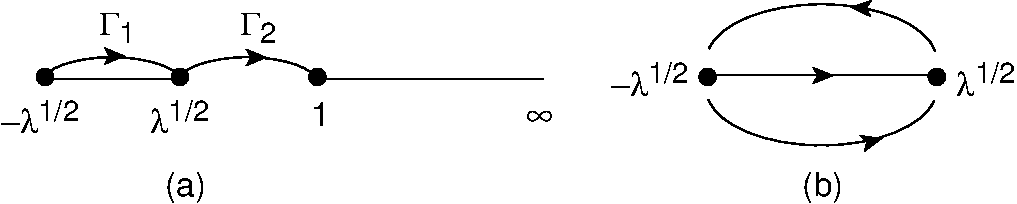
\includegraphics[width=0.95\textwidth]{figures/fig6.pdf}
  \caption{$\lambda$ 平面上的分支点与积分路径。(a) 分支点 $-\lambda^{1/2},\ \lambda^{1/2},\ 1,\ \infty$
           及路径 $\Gamma_1,\Gamma_2$；(b) 围绕 $\pm\lambda^{1/2}$ 的闭合路径及其定向。原文仅标
           “Figure 6”（原文 PDF 第 77 页），无说明性图注。}
  \label{fig:6}
\end{figure}

\begin{figure}[htbp]
  \centering
  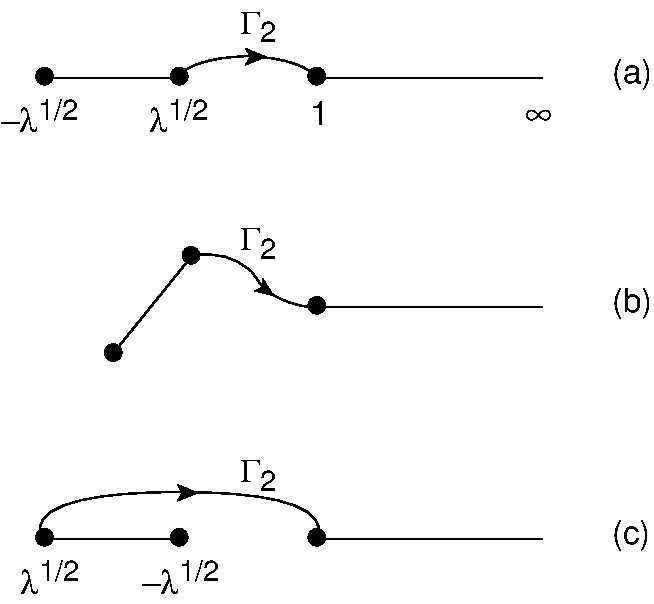
\includegraphics[width=0.55\textwidth]{figures/fig7.pdf}
  \caption{路径 $\Gamma_2$ 的变形。(a) $\lambda$ 平面上的 $\Gamma_2$；(b) 绕过分支点 $1$ 的变形；
           (c) 等价路径表示。原文仅标 “Figure 7”（原文 PDF 第 77 页），无说明性图注。}
  \label{fig:7}
\end{figure}

给定任意多项式，一个有用的量是它的判别式，定义为
$$
\Delta = \prod_{i<j} (e_i - e_j)^2,
$$
其中 $e_i$ 是根。$\Delta$ 可以用多项式的系数表达。显然，在两个分支点重合
的奇点处 $\Delta = 0$（$\infty$ 处的奇点除外）。例如对
$y^2 = (x-1)(x^2-u^n)$，在 $u = 0$ 附近 $\Delta \sim u^n$，而单值变换
共轭于 $T^n$。因此，在稳定情形下，单值变换的指数就是 $\Delta$ 的零点
阶数。例如，对由 (\ref{f2}) 描述的曲线族，$\Delta$ 在 $u=\pm\Lambda^2$
处有一阶零点，绕这些点的单值变换共轭于 $T$。
现在我们来看 $u\rightarrow \infty$。对大 $u$，分支点大约位于
$x=0,\,\Lambda^4/4u,\,u,\,\infty$。因此 $u=\infty$ 处的奇点不稳定，因为
在这一极限下多于两个分支点重合。这可以通过变量代换
$$
x = x'u\,, \qquad y = y' u^{3/2}\,,
$$
来修正，它把分支点移到 $0,\,\Lambda^4/4u^2,\,1,\,\infty$。判别式现在
表现为 $\Delta \sim u^{-4}$，对应共轭于 $T^{-4}$ 的单值变换。由于
$y \rightarrow y'$ 中存在 $\sqrt u$，用原来的变量 $(x,y)$ 表示时，单值
变换多出一个负号，共轭于 $PT^{-4}$。于是我们看到，曲线 (\ref{f2}) 给出
了 $N_f = 0$ 理论的正确单值变换。

% [Tutor Note: 见原文 PDF 第 77 页。$u\to\infty$ 处的奇点“不稳定”指
% 多于两个分支点重合。用 $x=x'u,\ y=y'u^{3/2}$ 把分支点移到有限位置后，
% 判别式在 $(x',y')$ 变量下表现为 $\Delta\sim u^{-4}$，对应共轭于
% $T^{-4}$ 的单值变换；但 $y=y'u^{3/2}$ 中的 $u^{3/2}$ 含有 $\sqrt u$，
% 绕 $u=0$ 一圈会给出额外的 $-1$，故回到原变量 $(x,y)$ 后单值变换是
% $PT^{-4}$ 而不是 $T^{-4}$（$P=-1$ 即宇称）。漏掉这个负号、把结果写成
% $T^{-4}$ 是最常见的错误。另外注意判别式的定义不含首项系数与整体符号，
% 与某些文献的约定相差常数因子。]

为了得到非零 $N_f$ 理论的曲线，我们应当知道这些理论中出现的单值变换。
这可以容易地算出来（如同 $N_f=0$ 情形），因为我们已经知道在 $u$ 平面
奇点处变为无质量的粒子的电荷谱。首先注意，如同 $N_f=0$ 理论，
$u=\infty$ 处的单值变换可以由微扰 $\beta$ 函数 (\ref{betanf})、或等价
地由 (\ref{betanf-mon}) 得到，结果为
$$
{\cal M}_{\infty} = PT^{N_f -4}.
$$
$u$ 平面有限点处的奇点一般对应无质量的磁单极，它们带一个单位的磁荷和
$n_e$ 个单位的电荷。为计算相应的单值变换，我们必须转到理论的对偶描述，
在其中磁单极与对偶规范场的耦合方式如同电子与通常规范场的耦合。在这一
框架下，单值变换由含 $k$ 个超多重态的单圈 QED $\beta$ 函数
(\ref{beta-hyper}) 决定，并由 $T^k$ 给出。这还必须与 $T^{n_e}S$ 共轭，
后者把荷为 $(0,1)$ 的超多重态变成荷为 $(1,n_e)$ 的磁单极。因此绕一个有
$k$ 个 $(n_m = 1, n_e)$ 磁单极的点的单值变换是
$(T^{n_e}S) T^k (T^{n_e}S)^{-1}$。类似的论证可用于计算 $N_f = 3$ 理论
中 $(2,1)$ 态的单值变换。下面我们列出上一小节描述的奇点周围的所有单值
变换：
$$
\begin{array}{rl}
N_f=0:& STS^{-1},\,(T^2 S)T(T^2 S)^{-1}\rightarrow M_{\infty}=PT^{-4}\,,\\
N_f=1:& STS^{-1},\,(TS)T(TS)^{-1},\, (T^2S)T(T^2S)^{-1} \rightarrow
M_{\infty}=PT^{-3}\,, \\
N_f=2:& ST^2 S^{-1},\,(TS)T^2(TS)^{-1}\rightarrow M_{\infty}=PT^{-2}\,,\\
N_f=3:& (ST^2S)T(ST^2S)^{-1},\,ST^4 S^{-1}\rightarrow
M_{\infty}=PT^{-1}\,. \\
\end{array}
$$
利用 $S^2=-1$ 与 $(ST)^3=1$，很容易验证对每个 $N_f$，有限 $u$ 处单值
矩阵的乘积都给出 $M_{\infty}$。注意在前三种情形（$N_f = 0,1,2$）中，
赋给奇点的电荷与我们先前论证所确定的电荷在符号上不同。这与把普适电荷和
群中心下的变换性质相联系时固有的不确定性一致。基于目前获得的知识，下面
我们概述 Seiberg 与 Witten 得到非零 $N_f$ 理论曲线显式形式的论证。

% [Tutor Note: 见原文 PDF 第 78 页。原文“massless magnetic monopoles with
% one unit of magnetic charge and $n_e$ units of magnetic charge”中第二个
% “magnetic charge”应为“electric charge”：磁单极带一个单位的磁荷与
% $n_e$ 个单位的电荷，这正是 $(n_m,n_e)=(1,n_e)$ 的含义。系原文笔误，
% 译文按正确含义（电荷）译出。另注意上表的单值矩阵之积给出
% $M_\infty=PT^{N_f-4}$，可用 $S^2=-1$、$(ST)^3=1$ 逐项核验；它是后面
% 确定各曲线形式的主要约束。]

\noindent\underline{$N_f =0$ 曲线的性质}：
在继续之前，列举 $N_f=0$ 曲线的一些性质非常有用，这些性质预期对非零
$N_f$ 仍然成立：
\begin{enumerate}
\item
描述曲线族的方程取一般形式 $y^2=F(x,u,\Lambda)$，其中 $F$ 是 $x$ 与 $u$
的不超过三次的多项式。
\item
$F$ 中关于 $x$ 与 $u$ 三次的部分是 $F_0 = x^2 (x-u)$。
\item
若给 $u$ 与 $x$ 赋 $U(1)_{\cal R}$ 荷 $4$、给 $\Lambda$ 赋荷 $2$，则
$F$ 的荷为 $12$。若给 $y$ 赋荷 $6$，则曲线在 $U(1)_{\cal R}$ 变换下
不变。
\item
$F$ 可以写成 $F = F_{0} + \Lambda^4 F_1$，其中 $F_1 = x/4$。
\end{enumerate}

性质 (1) 对 $N_f > 0$ 仍是一个拟设。它将给出正确的单值矩阵，并且在考虑
$N_f = 4$ 理论时也能部分地得到证明。性质 (2) 是下述事实的推论：当
$u \rightarrow \infty$ 时，我们必须得到与 $a_D$ 中来自单圈 $\beta$ 函数
的对数相联系的无穷远单值变换。这意味着有限 $x$ 处的某一个分支点应当在
$u\rightarrow\infty$ 时移到无穷远。对大 $u$，三次部分可以写成
$(x-e_1 u)(x-e_2 u)(x-e_3 u)$。于是，若两个 $e_i$ 相等而另一个不同（比如
$e_1=e_2\not=e_3$），就可得到所期望的行为。在这种情况下，通过重新定义
$x$，可以把 $F_0$ 化成 $x^2 (x-u)$ 的形式。性质 (4) 在 $N_f = 0$ 理论中
是 $U(1)_R$ 荷赋值的推论。注意 $F$ 只有一项经典贡献加上一项单瞬子项：
$\Lambda^4 x/4$。现在我们用这些性质来确定 $N_f = 1,2,3$ 的曲线。

\noindent\underline{无质量 $N_f=1$ 理论的曲线}：
在这个理论中，由方程 (\ref{inst-nf})，瞬子振幅正比于 $\Lambda^3_{1}$。
然而对 $N_f \geq 1$，瞬子因子在 $\rho$ 宇称下为奇，因此 $F$ 中只能出现
它的偶次幂。由于 $\Lambda_{1}$ 的 $U(1)_R$ 荷为 $2$、$F$ 的荷为 $12$，
唯一的可能是
$$
y^2 = x^2 (x-u) + t \Lambda^{6}_{1} \,.
$$
常数 $t$ 可以吸收到 $\Lambda_{1}$ 的重定义中：
$t\Lambda^{6}_{1}=\tilde{\Lambda}^6$。这一曲线族的判别式为
$$
\Delta = \tilde{\Lambda}^{6}_{1} (4 u^3 - 27 \tilde{\Lambda}^{6}_{1})\,.
$$
它有三个零点，这些零点在作用在 $u$ 平面上的 ${\bf Z}_3$ 变换下互相
交换，相应的单值变换共轭于 $T$。类似地，大 $u$ 处的单值变换可以算出为
$PT^{-3}$。这与 $N_f=1$ 理论应有的结果一致。

% [Tutor Note: 见原文 PDF 第 79 页。可用三次式 $x^3-ux^2+\tilde\Lambda^6$
% 的判别式 $\Delta=4u^3\tilde\Lambda^6-27\tilde\Lambda^{12}$ 核验此式：
% $x^3+ax^2+bx+c$ 的判别式为 $a^2b^2-4b^3-4a^3c-27c^2+18abc$，代入
% $a=-u,\ b=0,\ c=\tilde\Lambda^6$ 即得。注意原文的 $\Delta$ 定义不含
% 首项系数，与某些文献相差一个常数因子；零点位置（$u^3=\frac{27}{4}
% \tilde\Lambda^6$，三个零点相差 ${\bf Z}_3$ 相位）才是物理上重要的。]

\noindent\underline{无质量 $N_f=2$ 理论的曲线}：
在这种情况下瞬子因子是 $\Lambda^{2}_{2}$，同样，在没有裸质量时，$F$ 中
只能出现它的偶次幂。由于 $\Lambda_2$ 的 $U(1)_R$ 荷为 2，曲线的一般形式为
$$
y^2 = x^2 (x-u) + (ax + bu) \Lambda^{4}_{2}\,.
$$
根据我们对 $N_f=2$ 理论的讨论，预期有两个奇点，每个奇点带两个无质量磁单极。
因此每个奇点处的单值变换共轭于 $T^2$，这意味着每个有限奇点处的判别式
应当有二阶零点。这一条件确定了 $a$ 与 $b$。在对 $\Lambda_2$ 作重新标度
之后，$N_f=2$ 曲线族可以写成
$$
y^2 = (x^2 - \tilde{\Lambda}^{4}_{2} ) (x-u)\,,
$$
它具有所预期的 ${\bf Z}_2$ 对称性。

% [Tutor Note: 见原文 PDF 第 79 页。注意 $(x^2-\tilde\Lambda_2^4)(x-u)
% = x^3-ux^2-\tilde\Lambda_2^4x+u\tilde\Lambda_2^4$ 确实具有上式的
% “$(ax+bu)\Lambda_2^4$”形式：$a=-1,\ b=1$。所谓“判别式在每个有限奇点
% 处有二阶零点”即 $\Delta$ 有两个二重零点（对应两个奇点各两个无质量
% 单极），这正好确定两个系数 $a,b$。原文省略了这一代数步骤。]

\noindent\underline{无质量 $N_f=3$ 理论的曲线}：
在这种情况下，$u$ 平面上有两个奇点，其单值变换分别共轭于 $T^4$ 与 $T$，
并且没有对称性作用在 $u$ 平面上。取 $T^4$ 奇点在 $u = 0$。于是判别式
应在 $u=0$ 处有四阶零点。这与通常的 $U(1)_{\cal R}$ 荷及 $\rho$ 宇称
赋值一起给出
$$
F = a \Lambda^{2}_{3} x^2 + bu^2 x + cu x^2 + x^3 \,.
$$
这里 $b \not= 0$，否则曲线对所有 $u$ 都是奇异的。要求 $F$ 的三次部分
具有所期望的经典行为，并经过一些重新标度后，得到
$$
y^2 = x^2 (x-u) + \tilde {\Lambda}^{2}_{3} (x-u)^2\,.
$$

% [Tutor Note: 见原文 PDF 第 79--80 页。原文只给出拟设与最终曲线，中间
% “要求三次部分具有经典行为”和“经过一些重新标度”两步完全没有展开：
% 由 $F=x^3+(a\Lambda_3^2+cu)x^2+bu^2x$ 算判别式可得
% $\Delta=b^2u^4[(a\Lambda_3^2+cu)^2-4bu^2]$，在 $u=0$ 处的四阶零点由
% $b^2u^4$ 自动给出（$b\ne0$），这解释了下文“$b\not=0$”的条件；而
% $x$、$y$ 的允许重参数化（含 $x$ 的平移/标度）会把拟设化为最终形式。
% 原文未展示这些步骤，若需复现请参看 [32] 的严格处理。]

注意上面我们只考虑了没有裸质量项的理论。由于质量项具有奇的 $\rho$-宇称，
在有非零裸质量的理论中，瞬子因子的奇次幂也可以对曲线方程有贡献。我们在此
不讨论这些情形，但为完整起见，直接列出最终结果：
\begin{eqnarray}
N_f=1:\qquad y^2 &=& x^2(x-u)+ \frac{1}{4}m\Lambda_1^3 x -
\frac{1}{64} \Lambda_1^6\,, \nonumber \\
N_f=2:\qquad y^2 &=& (x^2-\frac{1}{64}\Lambda_2^4) (x-u) + m_1 m_2
\Lambda_2^2 x - \frac{1}{64}(m_1^2+m_2^2)\Lambda_2^4\,,\nonumber \\
N_f=3:\qquad y^2 &=& x^2(x-u)-\frac{1}{64} \Lambda_3^2(x-u)^2
-\frac{1}{64}(m_1^2+m_2^2+m_3^2) \Lambda_3^2(x-u) \nonumber \\
      && +\frac{1}{4}m_1m_2m_3 \Lambda_3 x - \frac{1}{64}
(m_1^2 m_2^2 + m_2^2 m_3^2 + m_1^2 m_3^2)\Lambda_3^2\,. \nonumber
\end{eqnarray}
关于更多细节与讨论（包括 $N_f=4$ 情形），以及得到曲线方程的更严格方法，
读者可参阅 Seiberg 与 Witten 的原始工作 \cite{SW2}。

% [Tutor Note: 见原文 PDF 第 80 页。这三条曲线在原书中全部带 nonumber
% 标注，因此不占公式编号，但它们与前面无质量曲线的关系可以
% 逐项核验：$m_i\to0$ 时 $N_f=1$ 给出 $-\frac1{64}\Lambda_1^6$（对应
% $t=-1/64$），$N_f=2$ 给出 $(x^2-\frac1{64}\Lambda_2^4)(x-u)$（对应
% $\tilde\Lambda_2^4=\frac1{64}\Lambda_2^4$），$N_f=3$ 给出
% $-\frac1{64}\Lambda_3^2(x-u)^2$（对应
% $\tilde\Lambda_3^2=-\frac1{64}\Lambda_3^2$，故 $\tilde\Lambda_3^2$
% 的符号与 $\Lambda_3^2$ 相反）。核对符号时以这一极限为依据。]

一旦曲线确定，其余步骤就与 $N_f=0$ 情形非常相似。我们通过围道积分定义
量 $a$ 与 $a_D$：
$$
a=\int_{\gamma_1} \, \lambda\,,\quad a_D=\int_{\gamma_2}\lambda\,,
$$
度规由 ${\rm Im}(\tau)$ 给出，其中 $\tau=\frac{da_D}{du}/
\frac{da}{du}$。这里 $\lambda$ 是一个全纯一形式，满足
$$ 
\frac{d\lambda}{du}=\frac{\sqrt 2}{8\pi}\frac{dx}{y}\,.
$$
与 $N_f=0$ 情形的差别在于，现在 $\lambda$ 可以有非零留数的极点，不过
留数应当与 $u$ 无关。若如此，则 $\tau$ 仍经历 $SL(2,Z)$ 变换，而
$(a_D, a)$ 经历 $SL(2,Z)$ 变换外加一个移动。正如我们在带非零裸质量夸克的
QED 情形所看到的，这一移动实际上是必需的，并且与修改后的 BPS 质量公式
(\ref{bps-m}) 一致。由此推出，造成移动的 $\lambda$ 的留数应当正比于裸
夸克质量。这一点已在 \cite{SW2} 中对 $N_f=2$ 曲线作了检验，并发现确实
如此。事实上，留数的存在具有很强的限制性，Seiberg 与 Witten 正是利用
这一信息以严格的方式导出了 $N_f=4$ 理论的曲线。其他理论的曲线则可以由
重整化群流确定，结果与上面所列一致。

% [Tutor Note: 见原文 PDF 第 80 页。$d\lambda/du$ 的系数
% $\sqrt2/(8\pi)$ 中含因子 $\sqrt2$ 与 $8\pi$，与式 (109)
% 的 $1/2\pi$、式 (111) 的 $1/16\pi^2$ 相互关联；改动任何一处
% 归一化都会破坏周期 $a,a_D$ 与单值矩阵的一致性，抄写时必须逐字符核对。
% 另外原文“used by Seiberg and Witten to drive the curve”中的“drive”
% 系“derive”（导出）的拼写笔误；同页“varialbles”（应为 variables）、
% “form the perturbative”（应为 from）等亦为排印笔误。全片类似的拼写
% 笔误还有 sigularities（应为 singularities，第 74--75 页）、
% analoguous（应为 analogous，第 73 页）、representaion（应为
% representation，第 73 页），译文均已按正确词义处理。留数正比于裸质量
% 是本节与前面 QED 讨论（$a_D$ 的平移）相呼应的关键结论。]

   % §4 与 §4.1--§4.6（原文 PDF 65--80 页）

%---------------------- 致谢与参考文献 ----------------------
%=====================================================================
%  致谢（Lead 翻译，原文 PDF 第 80 页）
%=====================================================================
\section*{致谢}
\markboth{致谢}{}
\addcontentsline{toc}{section}{致谢}

在本讲义所涉主题上，我们与同事们的无数次讨论使我们受益良多。我们尤其要感谢
E. Alvarez、S. Randjbar-Daemi、W. Lerche、A. Klemm、S. Yankielowicz、C. Gomez、
K. Kounnas、M. Mari\~no、J. Distler、E. Verlinde、A. Giveon、E. Rabinovici 与
G. L. Cardoso 的有益讨论。我们还要感谢的里雅斯特理论组（Trieste Theory Group）
提供机会，让我们在富有激励的环境中讲授这些内容。

% [Tutor Note: 原文致谢中的 “Trieste Theory Group” 即 ICTP 的里雅斯特理论组；本讲义源自
% 1995 年 Trieste Summer School 的系列讲座（见原文 PDF 第 2 页引言第一段），故致谢对象与
% 讲座背景一致。]
   % 致谢
%% =====================================================================
%%  参考文献（保留原文条目，不译；编号由 thebibliography 自动生成，
%%  与原文 [1]--[40] 逐一对应）
%% =====================================================================
\section*{参考文献}
\markboth{参考文献}{}
\addcontentsline{toc}{section}{参考文献}
\begin{thebibliography}{100}
\bibitem{GO}
P. Goddard and D. I. Olive, Rep. Prog. Phys. {\bf 41} (1978) 1357.
\bibitem{coleman1}
S. Coleman, {\it Classical Lumps and Their Quantum Descendants}, In
the Proc. of the 1975 Int. School of Subnuclear Physics, Erice;
Ed. A. Zichichi, Plenum Press (1977).  
\bibitem{coleman2}
S. Coleman, {\it The Magnetic Monopole Fifty Years Later}, In the
Proc. of the 1981 Int. School of Subnuclear Physic, Erice;
Ed. A. Zichichi, Plenum Press (1983).
\bibitem{Dirac}
P. A. M. Dirac, Phys. Rev. {\bf 74} (1948) 817.
\bibitem{Goldhaber}
A. S. Goldhaber, Phys. Rev. Lett. {\bf 36} (1976) 1122.
\bibitem{Wilczek}
F. Wilczek, Phys. Rev. Lett. {\bf 48} (1982) 1146.
\bibitem{Schwinger}
J. Schwinger, Phys. Rev. {\bf 144} (1966) 1087; {\bf 173} (1968)
1536. 
\bibitem{Zwanziger}
D. Zwanziger, Phys. Rev. {\bf 176} (1968) 1480.
\bibitem{thooft}
G. 't Hooft, Nucl. Phys. {\bf B79} (1974) 276. 
\bibitem{polya}
A. M. Polyakov, JETP Lett. {\bf 20} (1974) 194.
\bibitem{Julia-Zee}
B. Julia and A. Zee, Phys. Rev. {\bf D11} (1975) 2227.
\bibitem{TW1}
E. Tomboulis and G. Woo, Nucl. Phys. {\bf B107} (1976) 221.
\bibitem{GSW}
J. L. Gervais, B. Sakita and S. Wadia, Phys. Lett. {\bf 63B} (1976) 55. 
\bibitem{bogomol}
E. B. Bogomol'nyi, Sov. J. Nucl. Phys. {\bf 24} (1976) 449.
\bibitem{PS}
M. K. Prasad and C. M. Sommerfield, Phys. Rev. Lett. {\bf 35} (1975)
760. 
\bibitem{CO}
E. Corrigan and D. Olive, Nucl. Phys. {\bf B110} (1976) 237.
\bibitem{GNO}
P. Goddard, J. Nuyts and D. Olive, Nucl. Phys. {\bf B125} (1977) 1.
\bibitem{MO}
C. Montonen and D. Olive, Phys. Lett. {\bf 72B} (1977) 117.
\bibitem{manton}
N. S. Manton, Nucl. Phys. {\bf B126} (1977) 525.
\bibitem{sen}
A. Sen, Phys. Lett. {\bf 329B} (1994) 217.
\bibitem{Witten79}
E. Witten, Phys. Lett. {\bf 86B} (1979) 283.
\bibitem{WB}
J. Wess and J. Bagger, {\it Supersymmetry and Supergravity}, Princeton
University Press (1983).
\bibitem{West}
P. West, {\it Introduction to Supersymmetry and Supergravity}, World
Scientific, Singapore (1990).
\bibitem{Sohnius}
M. Sohnius, Phys. Rep. {\bf 128} (1985) 39.
\bibitem{HLS}
R. Haag, J. T. Lopuszanski and M. Sohnius, Nucl. Phys. {\bf B88}
(1975) 257.
\bibitem{Olive-Witten}
E. Witten and D. Olive, Phys. Lett. {\bf 78B} (1978) 97.
\bibitem{Grimm}
R. Grimm, M. Sohnius and J. Wess, Nucl. Phys. {\bf B133} (1978) 275.
\bibitem{bilal}
A. Bilal, {\it Duality in N=2 SUSY SU(2) Yang-Mills Theory: A
Pedagogical Introduction to the Work of Seiberg and Witten},
hep-th/9601007. 
\bibitem{DDS}
A. C. Davis, M. Dine and N. Seiberg, Phys. Lett. {\bf 125B} (1983) 487.
\bibitem{ADS}
I. Affleck, M. Dine and N. Seiberg, Nucl. Phys. {\bf B241} (1984) 493.
\bibitem{SW-I}
N. Seiberg and E. Witten, Nucl. Phys. {\bf B426} (1994) 19.
\bibitem{SW2} 
N. Seiberg and E. Witten, Nucl. Phys. {\bf B431} (1994) 484. 
\bibitem{Seiberg88}
N. Seiberg, Phys. Lett. {\bf 206B} (1988) 75.
\bibitem{DD}
A. D'adda and P. DiVecchia, Phys. Lett. {\bf 73B} (1978) 162.
\bibitem{GR}
I. S. Gradshteyn and I. M. Ryzhik, {\it Table of Integrals, Series and
Products}, Academic Press (1980).
\bibitem{SV1}
M. A. Shifman, A. I. Vainshtein, Nucl. Phys. {\bf B277} (1986) 456.
\bibitem{SV2}
M. A. Shifman and A. I. Vainshtein, Nucl. Phys. {\bf B359} (1991) 571.
\bibitem{Seiberg-n}
N. Seiberg, Phys. Lett. {\bf 318B} (1993) 469.
\bibitem{Seiberg-poh}
N. Seiberg, {\it Power of Holomorphy - Exact Results in 4-D
Supersymmetric Gauge Theories}, hep-th/9408013. 
\bibitem{Lerche}
W. Lerche, {\it Introduction to Seiberg-Witten Theory and its Stringy
  Origin}, In the proceedings of the 1996 Trieste spring school on
String Theor, hep-th/9611190.  
\end{thebibliography}


%---------------------- 附录：审校批注索引（由脚本生成） ----------------------
\IfFileExists{notes_index.tex}{% =====================================================================
%  附录：审校批注索引
%  由工具从正文各分片中的 % [Tutor Note: ...] 自动汇总生成；
%  源码中的批注为 LaTeX 注释，编译后不显示，此处以正文形式列出。
% =====================================================================
\newpage
\section*{附录　审校批注索引}
\addcontentsline{toc}{section}{附录　审校批注索引}
\markboth{附录　审校批注索引}{}
\noindent\small
本附录把正文源码中的 \verb|% [Tutor Note: ...]| 批注按章节顺序汇总，便于不读源码时检索。
每条批注前标出所属小节；若批注本身注明页码，则在括注中给出原文电子底本的页码
（原文印刷页号 $=n-1$）。
\normalsize

\par\medskip\noindent\hangindent=3.2em\hangafter=1 \textbf{[1]}~\textbf{引言}~见原文 PDF 第 2 页引言第一段。文中“Trieste Summer School”指 1995 年在意大利的里雅斯特（Trieste）举办的暑期学校系列讲座，本讲义即这些讲座的整理稿；原文称其为“very late written version”（很晚才写成的版本），故译作“成文远晚于讲座本身”。
\par
\par\medskip\noindent\hangindent=3.2em\hangafter=1 \textbf{[2]}~\textbf{引言}~见原文 PDF 第 3 页引言第二段。原文称含物质时“the duality group is no longer pure $SL(2,Z)$”，其中“pure”指对偶群不再是整个 $SL(2,Z)$，而是它的真子群（同余子群）；具体形式与物质场的味数 $N_f$ 有关，详见原文第 4.6 节（原文 PDF 第 75 页起）。
\par
\par\medskip\noindent\hangindent=3.2em\hangafter=1 \textbf{[3]}~\textbf{1.1}~见原文 PDF 第 3 页式 (1)。此处采用的是 $c=\hbar=1$ 且库仑定律带因子 $(4\pi)^{-1}$ 的“有理化”单位制（Lorentz–Heaviside 型），故点电荷场强为 $\vec{E}=q\vec{r}/4\pi r^{3}$ 而非 $q\vec{r}/r^{3}$。后文的 $4\pi$、$e=q/\hbar$ 以及磁荷 $g$ 的归一化全都由它确定；若换用 SI 或高斯制，电荷量子化条件会整体差一个 $4\pi$，核对时请务必以此单位制为准。
\par
\par\medskip\noindent\hangindent=3.2em\hangafter=1 \textbf{[4]}~\textbf{1.1}~见原文 PDF 第 3 页式 (2) 与第 4 页式 (3)。在号差 $(+,-,-,-)$、$\varepsilon^{0123}=+1$ 下，$F_{0i}=E^i$ 但升指标得 $F^{0i}=-E^i$，同理 $\widetilde F^{0i}=-B^i$；式 (3) 的两个矩阵里 $E$、$B$ 的符号分布正是这一约定的结果，此处是最容易漏掉负号的地方，请逐项核对。
\par
\par\medskip\noindent\hangindent=3.2em\hangafter=1 \textbf{[5]}~\textbf{1.1}~见原文 PDF 第 4 页式 (5)、(6)。要点有二：其一，对偶不变性只在场与流“同时”按式 (6) 变换时才成立，单独变换场并不是麦克斯韦方程组的对称性；其二，原文所说连续的 $SO(2)$ 群指 $(F,\widetilde F)$ 平面内的转动（等价于对复组合 $F+i\widetilde F$ 作相位变换），这正是后文 $S$ 对偶连续版本的雏形。
\par
\par\medskip\noindent\hangindent=3.2em\hangafter=1 \textbf{[6]}~\textbf{1.2}~见原文 PDF 第 5 页式 (8)。第二个等号是分部积分：$\partial_j\hat{x}^i=(\delta_{ij}-x_ix_j/r^2)/r$，再把 $E^j\partial_j\hat{x}^i$ 写成 $\partial_j(E^j\hat{x}^i)-\hat{x}^i\partial_j E^j$。原文只说“球对称使第一个积分消失”，对真正给出式 (9) 的 $\vec{\nabla}\cdot\vec{E}=q\delta^{3}(\vec{r})$ 一项轻轻带过——恰恰是原点处的 $\delta$ 源贡献了 $-qg/4\pi\,\hat{r}$。这是本段最容易“差一个符号”的地方，请按 $\partial_j\hat{x}^i$ 的符号重新核对。
\par
\par\medskip\noindent\hangindent=3.2em\hangafter=1 \textbf{[7]}~\textbf{1.2}~见原文 PDF 第 6 页式 (10) 前一句。原文“if we assume that orbital angular momentum is quantized. Then it follows that”在句号处应作逗号（原文标点笔误），译文的句式已按正确逻辑重写。物理上这里假设的是“总角动量（含场角动量 $\vec{J}_{em}$）以 $n\hbar/2$ 量子化”，而非纯轨道角动量；随后原文承认这与两个组元都是玻色子相矛盾，并把解释归于文献 [5,6]（Goldhaber、Wilczek）。下一小节由狄拉克弦给出的推导不依赖此假设。
\par
\par\medskip\noindent\hangindent=3.2em\hangafter=1 \textbf{[8]}~\textbf{1.2}~见原文 PDF 第 6 页式 (13)。注意 $n_{12}$ 依赖两粒子的编号顺序，交换 $1\leftrightarrow2$ 时 $n_{12}\to-n_{12}$；而 $q_1g_2-q_2g_1$ 正是二维矢量 $(q_i,g_i)$ 的行列式，在 $(q_i,g_i)$ 整体 $SO(2)$ 转动下不变。这一“量子化条件与连续对偶相容”的事实，正是后文（§4）把对偶群视为 $SL(2,Z)$ 的子群、并研究其单值变换的出发点。
\par
\par\medskip\noindent\hangindent=3.2em\hangafter=1 \textbf{[9]}~\textbf{1.3}~见原文 PDF 第 7 页第 2 行。原文写 $\vec{B}_{mon}=\vec{\nabla} \vec{A}_{mon}$，漏掉叉乘号，应为 $\vec{B}_{mon}=\vec{\nabla}\times\vec{A}_{mon}$（原文笔误，译文照录）。正因为磁单极场满足 $\vec{\nabla}\cdot\vec{B}_{mon}\ne 0$，这样的 $\vec{A}_{mon}$ 才无法整体存在。
\par
\par\medskip\noindent\hangindent=3.2em\hangafter=1 \textbf{[10]}~\textbf{1.3}~见原文 PDF 第 7 页式 (14)。其中 $g/4\pi r^{2}$ 一项应为 $g\hat{r}/4\pi r^{2}$（即 $\vec{B}_{mon}=g\vec{r}/4\pi r^{3}$），原文漏写单位矢量 $\hat{r}$（原文笔误，译文照录）；补上它，$\vec{B}_{mon}$ 的方向信息才完整，也才能与 $\vec{\nabla}\cdot\vec{B}_{mon}=g\delta^{3}(\vec{r})$ 自洽。
\par
\par\medskip\noindent\hangindent=3.2em\hangafter=1 \textbf{[11]}~\textbf{1.3}~见原文 PDF 第 7 页“Aharonov–Bohm 相位”一段，紧接式 (14) 之后。相位 $e\oint_\Gamma\vec{A}_{sol}\cdot d\vec{l}=eg$ 中的 $e$ 是经 $\hbar$ 归一化的耦合常数 $e=q/\hbar$（原文如此，并非裸电荷），故 $eg=2\pi n$ 与上小节的 $qg/4\pi\hbar=n/2$ 完全等价；两种推导的一致性全靠这一归一化，切勿把 $e$ 当作 $q$ 代入。
\par
\par\medskip\noindent\hangindent=3.2em\hangafter=1 \textbf{[12]}~\textbf{1.4}~见原文 PDF 第 8 页“Derrick 定理”一句。原文只给结论，其证明是标度论证：对静态场作标度变换 $\phi_\lambda(\vec{x})=\phi(\lambda\vec{x})$，能量泛函可写成 $E(\lambda)=\lambda^{2-d}K+\lambda^{-d}V$（$K$ 为梯度项、$V$ 为势能项，均非负）；$d>1$ 时 $\mathrm{d}E/\mathrm{d}\lambda=0$ 无解，故 $d\ge2$ 的标量场论不存在静态有限能量解。原文另把这归因于孤立子在远距离处的非平凡结构，这是从位形角度的直观说法。
\par
\par\medskip\noindent\hangindent=3.2em\hangafter=1 \textbf{[13]}~\textbf{1.4}~见原文 PDF 第 8 页式 (15)、(16)。$W_\mu=W^a_\mu T^a$ 是矩阵值场，$G_{\mu\nu}=G^a_{\mu\nu}T^a$；用 $(T^a)_{bc}=-if^a_{bc}$ 与 $f^{abc}=\epsilon^{abc}$ 展开 $ie[W_\mu,W_\nu]$，得 $G^a_{\mu\nu}=\partial_\mu W^a_\nu-\partial_\nu W^a_\mu-e\epsilon^{abc}W^b_\mu W^c_\nu$。式中的因子 $i$ 与 $D_\mu\phi^a$ 里的 $-e$ 是配套的，符号弄反会直接改变式 (18) 的运动方程，并影响后文 BPS 界与磁荷的符号。
\par
\par\medskip\noindent\hangindent=3.2em\hangafter=1 \textbf{[14]}~\textbf{1.4}~见原文 PDF 第 9 页微扰谱表格。表中“Spin”一列对光子与 $W^\pm$ 填 $\hbar$、对 $H$ 填 $0$，这是原文的写法：自旋一栏理应填自旋量子数 $1,1,0$（即 $s\hbar$ 中的 $s$），原文直接填入 $\hbar$，单位上亦不自洽，属原文笔误；为与源公式块保持一致，表头 Mass/Spin/Charge 保留原文，译名即“质量/自旋/电荷”。表中 $W^\pm$ 的质量 $ae\hbar=aq$ 与电荷 $\pm q=\pm e\hbar$ 彼此一致。
\par
\par\medskip\noindent\hangindent=3.2em\hangafter=1 \textbf{[15]}~\textbf{1.4}~本片原文拼写笔误汇总（译文均按正确词义翻译，源文件未改）：p2 “intented”→intended；p3 “proporties”→properties、“Minkowsky”→Minkowski；p4 “quations”→equations；p5 “elecromagnetic”→electromagnetic；p6 “fermios”→fermions，且“both of the components are bosonic.”句首小写；p7 “intruduced”→introduced；p8 “satifying”→satisfying、“representaion”→representation、“cavariant”→covariant。另有句读笔误一处，见式 (10) 前的批注。
\par
\par\medskip\noindent\hangindent=3.2em\hangafter=1 \textbf{[16]}~\textbf{1.5}~见原文 PDF 第 9 页开头。有限能量条件为 $E=\int\theta_{00}\,d^3x<\infty$：三维体积元带来 $r^2dr$，故要求 $\theta_{00}$ 的衰减快于 $1/r^3$（而不是快于 $1/r^2$）；这里的 $\theta_{00}$ 在静态情形下就是能量密度。
\par
\par\medskip\noindent\hangindent=3.2em\hangafter=1 \textbf{[17]}~\textbf{1.5}~见原文 PDF 第 10 页式 (24)。此处系数最容易写错：第一项的 $1/(ea^2)$ 中 $a^2$ 来自 $\vec{\phi}_{vac}\cdot\vec{\phi}_{vac}=a^2$，第二项的 $1/a$ 保证 $A_\mu$ 是归一化的 $U(1)$ 规范场。代回式 (23) 时只需两个恒等式：$\vec{\phi}_{vac}\cdot\partial_\mu\vec{\phi}_{vac}=0$ 与 $(\vec{\phi}_{vac}\times\partial_\mu\vec{\phi}_{vac})\times\vec{\phi}_{vac}=a^2\partial_\mu\vec{\phi}_{vac}$。
\par
\par\medskip\noindent\hangindent=3.2em\hangafter=1 \textbf{[18]}~\textbf{1.5}~原文笔误，见原文 PDF 第 10 页式 (26) 之后。“Since $\phi^2=a$;”有两处问题：(1) 应为 $\phi^2=a^2$，与式 (23) 一致；(2) 分号应为逗号。译文照录公式原样，只按文意断句。
\par
\par\medskip\noindent\hangindent=3.2em\hangafter=1 \textbf{[19]}~\textbf{1.5}~见原文 PDF 第 10 页式 (28)。原文说它与狄拉克条件“相差因子 2”，核对如下：取 $q_0=e\hbar/2$，则 $g_\Sigma q_0/(4\pi\hbar)=-\nu/2$，而狄拉克条件为 $qg/(4\pi\hbar)=n/2$，故要求 $\nu=-n$。式 (26) 中的负号来自 $B^i=-\frac{1}{2}\epsilon^{ijk}F_{jk}$ 与曲面定向的约定，不要与式 (27) 中 $\nu$ 的符号约定混为一谈。
\par
\par\medskip\noindent\hangindent=3.2em\hangafter=1 \textbf{[20]}~\textbf{1.5}~见原文 PDF 第 11 页式 (29) 之后。核对边界条件：$r\to0$ 时 $H\sim\xi$ 使 $\phi^a=(x^a/er^2)H\to c_1x^a\to0$，故场在原点正则；$r\to\infty$ 时 $H\sim\xi$ 给出 $\phi^a\to ax^a/r=a\hat{x}^a$，而 $K\to0$ 给出 $W^a_i\to-\epsilon^a_{ij}x^j/er^2$。注意 $H$、$K$ 的自变量是 $\xi=aer$ 而不是 $r$，做量纲核对时不要丢掉 $e$ 与 $a$。
\par
\par\medskip\noindent\hangindent=3.2em\hangafter=1 \textbf{[21]}~\textbf{1.5}~原文 PDF 第 11 页这一段有数处拼写笔误：“easiy”应为“easily”，“guage”应为“gauge”，“treate”应为“treat”，“depends of”应为“depends on”；译文均按原意处理。关于集体坐标论证：静态双子解带有一个连续参数（即 $W^a_0$ 的系数），它对应于保持希格斯真空的 $U(1)$ 规范方向的零模；把该规范自由度作为集体坐标量子化后，其共轭动量（电荷）取分立值 $q=n\hbar e$，细节见文献 [12,13]。
\par
\par\medskip\noindent\hangindent=3.2em\hangafter=1 \textbf{[22]}~\textbf{1.6}~见原文 PDF 第 12 页式 (30)。把面积分化为体积分用了两个不同方程：磁荷用非阿贝尔比安基恒等式 $D_i{\cal B}^a_i=0$，电荷用高斯定律（即 (\ref{XXIX}) 的第一个方程）。注意等号链中“面积分”与“体积分”之间的那一步并不只是把 $a$ 提出：需要把 $\phi^a/a$ 作为单位矢量场、分部积分并用 $D_i{\cal B}^a_i=0$，才能把被积函数中的 $\phi^a$ 换成 $(D^i\phi)^a$；这是本节最容易被读者一带而过的地方。
\par
\par\medskip\noindent\hangindent=3.2em\hangafter=1 \textbf{[23]}~\textbf{1.6}~易错预警，见原文 PDF 第 12 页式 (31)。平方配方时务必与式 (30) 中 $g,q$ 的定义对照：把方括号内展开，除保留 $\frac12[({\cal E}^a_k)^2+({\cal B}^a_k)^2+(D_k\phi^a)^2+(D_0\phi^a)^2]$ 外，交叉项为 $-\sin\theta\,{\cal E}\cdot D\phi-\cos\theta\,{\cal B}\cdot D\phi=-a(q\sin\theta+g\cos\theta)$（注意是负号！），移项后才得到式 (31) 末行的 $+a(q\sin\theta+g\cos\theta)$。若把交叉项符号弄反，就会得出 $M\le a\sqrt{q^2+g^2}$ 的错误结论。对 $\theta$ 求极值时用 $\tan\theta=q/g$，最大值为 $\sqrt{q^2+g^2}$。
\par
\par\medskip\noindent\hangindent=3.2em\hangafter=1 \textbf{[24]}~\textbf{1.6}~见原文 PDF 第 12 页。此处对 $\hbar$ 的处理较随意：由 $M_W=ae\hbar=aq$ 与 $\nu/\alpha$ 的写法可反推出 $\alpha\equiv q^2/(4\pi\hbar)$，只有取 $\hbar=1$ 时才与通常的 $\alpha=e^2/4\pi\sim1/137$ 相符。原文此处只作定性结论（磁单极远重于 W 玻色子），不必纠结 $\hbar$ 的幂次；$\nu=1$ 或 $1/4$ 则取决于把“电子电荷”取作 $q$ 还是 $q/2$。
\par
\par\medskip\noindent\hangindent=3.2em\hangafter=1 \textbf{[25]}~\textbf{1.6}~见原文 PDF 第 13 页。式 (32) 其实是两类一阶（BPS）方程的合写：$D_0\phi=0$ 与 $\vec{\cal E}=\sin\theta\,D\phi$、$\vec{\cal B}=\cos\theta\,D\phi$；把 't Hooft–Polyakov 拟设代入这些一阶方程即可精确求解（原文引 [14,15]）。另注意：$\lambda\to0$ 时 $V=0$，$a$ 不再由势的极小值固定，故 $|\phi|=a$ 只能作为边界条件强加，这一点在后文 Seiberg–Witten 分析中至关重要。
\par
\par\medskip\noindent\hangindent=3.2em\hangafter=1 \textbf{[26]}~\textbf{1.7}~术语与记号说明，见原文 PDF 第 13 页。原文用同一个字母 $g$ 表示两件完全不同的东西：群元素 $g$（如式 (36) 的 $g(s,t)$）与磁荷 $g$（见式 (30) 与式 (35)）。阅读时须按上下文区分，切勿把 $g(s,t)$ 的指标结构套到磁荷上。
\par
\par\medskip\noindent\hangindent=3.2em\hangafter=1 \textbf{[27]}~\textbf{1.7}~易错预警，见原文 PDF 第 14 页式 (35)。与 §1.6 的 $M\ge a\sqrt{g^2+q^2}$ 相比这里多出因子 $\sqrt2$：式 (33) 的希格斯动能是复标量的 $(D_\mu\phi)^\dagger D^\mu\phi$，平方配方时须写成 $\frac{1}{2}|{\cal E}-\sqrt2\,D\phi\sin\theta|^2$、$\frac{1}{2}|{\cal B}-\sqrt2\,D\phi\cos\theta|^2$ 之类的形式（实部、虚部各贡献一份），交叉项才给出 $\sqrt2\,a(q\sin\theta+g\cos\theta)$；若照搬 §1.6 实伴随场的 $\frac12(D\phi)^2$ 配方，就会漏掉这个 $\sqrt2$。
\par
\par\medskip\noindent\hangindent=3.2em\hangafter=1 \textbf{[28]}~\textbf{1.7}~含糊点拨，见原文 PDF 第 14 页。原文“$G_{\mu\nu}$ 取值于 $G$ 的某个子群”严格说应为“取值于该子群的李代数”；这里只是省略了“李代数”三字，物理内容不变。又：原文此处有重复词 “the the little group”，系笔误。
\par
\par\medskip\noindent\hangindent=3.2em\hangafter=1 \textbf{[29]}~\textbf{1.7}~原文笔误，见原文 PDF 第 14 页：“from this square to the sphare” 中 “sphare” 应为 “sphere”。
\par
\par\medskip\noindent\hangindent=3.2em\hangafter=1 \textbf{[30]}~\textbf{1.7}~图 2 的读法，见原文 PDF 第 15 页。$(s,t)$ 正方形的整个边界都映到基点 $r_0$，故对每个固定的 $s$，$t\in[0,1]$ 是 $\Sigma$ 上一条由 $r_0$ 出发又回到 $r_0$ 的闭曲线；右图中这些闭曲线按同伦类分层，其绕数即磁荷。注意左图中竖直箭头只表示 $t$ 增大方向，图中的“曲线族”是同一映射 $r(s,t)$ 在不同 $s$ 处的像。
\par
\par\medskip\noindent\hangindent=3.2em\hangafter=1 \textbf{[31]}~\textbf{1.7}~见原文 PDF 第 15 页式 (36)。$P$ 表示路径编序（沿 $t$ 增大方向）；指数中 $ie\int\vec{W}\cdot d\vec{r}$ 的量纲须与式 (33) 的 $D_\mu=\partial_\mu+ieW_\mu$ 一致，核对时勿额外添加 $e$ 或 $2\pi$。
\par
\par\medskip\noindent\hangindent=3.2em\hangafter=1 \textbf{[32]}~\textbf{1.7}~含糊点拨，见原文 PDF 第 16 页的正合序列。原文“$\pi_2(G)$ 可作为单位元嵌入 $\pi_2(G/H)$”的措辞不严谨：对紧致连通 $G$ 有 $\pi_2(G)=0$，于是由正合性得 $\pi_2(G/H)$ 单射地映入 $\pi_1(H)$，其像正是（在 $G$ 中同伦于平庸路径的）$\pi_1(H)_G$，故 $\pi_2(G/H)\cong\pi_1(H)_G$。原文所谓“嵌入”只是说明 $\pi_2(G)=0$ 这一环在序列中不贡献，读者不必按字面理解为群嵌入。完整讨论见文献 [2]（Coleman）。
\par
\par\medskip\noindent\hangindent=3.2em\hangafter=1 \textbf{[33]}~\textbf{1.7}~见原文 PDF 第 16 页。原文称“后面我们会证明 $g=4\pi N/e$”，但本分片后文并未再给出独立证明；读者可对照式 (37)–(42) 的广义量子化条件自行补出（比较 $h(t)$ 的指数中 $4\pi N/a$ 的归一化与式 (41) 中 $G_0$ 前的 $ie/4\pi$）。另注意半整数 $N$ 的路径在 $SO(3)$ 中虽闭合，却生成 $\pi_1(SO(3))={\bf Z}_2$ 的非平凡类，不在 $\pi_1(H)_G$ 中，故最终两种情形都只保留整数 $N$。
\par
\par\medskip\noindent\hangindent=3.2em\hangafter=1 \textbf{[34]}~\textbf{1.8}~含糊点拨，见原文 PDF 第 17 页。原文“the magnetic flux in a solid angle subtended at the origin by the path”措辞较绕：应理解成“穿过该路径所张立体角（以原点为顶点）的磁通量”，即 $\Omega(s)$ 本身是立体角、乘以 $B$ 才是通量；这正是 $\alpha(s)=d\Omega/ds$ 的几何含义。
\par
\par\medskip\noindent\hangindent=3.2em\hangafter=1 \textbf{[35]}~\textbf{1.8}~含糊点拨，见原文 PDF 第 18 页。原文“If all values of $n$ are allowed, then $U(1)\cap K\subset Z_N$”一步较绕：其含义是整体上 $H$ 不是直积 $U(1)\times K$，而是 $(U(1)\times K)/Z_N$ 型的结构，故 $U(1)$ 与 $K$ 的中心在整体上重合；对色单态（$k=1$）回到通常的狄拉克条件，而对色非单态则得到以 $1/N$ 为单位的分数电荷。注意原文用 $|s>$、$|c>$ 而不是 $|s\rangle$、$|c\rangle$，系作者笔误，译文照录。
\par
\par\medskip\noindent\hangindent=3.2em\hangafter=1 \textbf{[36]}~\textbf{1.9}~原文笔误，见原文 PDF 第 18 页：“the magnetic componenets”中 “componenets” 应为 “components”。
\par
\par\medskip\noindent\hangindent=3.2em\hangafter=1 \textbf{[37]}~\textbf{1.9}~见原文 PDF 第 18–19 页。由式 (42) 得到 $e\beta^a\omega^a\in2\pi{\bf Z}$ 后，$e\beta$ 落在与权格 $\Lambda(H)$ 对偶的格 $\Lambda^*(H)$ 上；原文随即把这个对偶格解释为对偶群 $H^v$ 的权格。这一步依赖 $H$ 的表示与归一化约定（原文也明说 “factors of $e$ and $2\pi$ are convention dependent”），下面 $SO(3)$ 与 $SU(2)$ 的例子正是用 $T^3$ 的整/半整本征值来体现这种约定依赖。
\par
\par\medskip\noindent\hangindent=3.2em\hangafter=1 \textbf{[38]}~\textbf{1.9}~原文笔误，见原文 PDF 第 19 页。本页有三处拼写错误：“weekly coupled”应为“weakly coupled”，“monoples”应为“monopoles”，“superysymmetry”应为“supersymmetry”；另有“in the in the $H^v$-theory”重复了“in the”（在原文 PDF 第 19 页下半页）。物理上注意：Montonen–Olive 猜想交换的是微扰谱中的基本粒子与孤子，即 $H$ 理论与 $H^v$ 理论互换，耦合常数 $q/\hbar\leftrightarrow g/\hbar$；在自对偶的 $H=U(1)=H^v$ 情形，这一互换表现为 $e\leftrightarrow g=4\pi/e$，即强耦合与弱耦合互换。
\par
\par\medskip\noindent\hangindent=3.2em\hangafter=1 \textbf{[39]}~\textbf{1.10}~原文笔误，见原文 PDF 第 20 页：“half-odd inegral values”中 “inegral” 应为 “integral”；译文按正确含义处理。
\par
\par\medskip\noindent\hangindent=3.2em\hangafter=1 \textbf{[40]}~\textbf{1.10}~易错预警，见原文 PDF 第 20–21 页。核对 $\theta$ 项的归一化：$F^a_{\mu\nu}\tilde F^{a\mu\nu}$ 是全导数，$\partial_\mu K^\mu=\frac12\epsilon^{\mu\nu\rho\sigma}F^a_{\mu\nu}F^a_{\rho\sigma}$，故式 (44) 中系数取 $\theta e^2/32\pi^2$ 才能保证 $\theta\to\theta+2\pi$ 是物理上等价的周期；若把 $\tilde F$ 的 $\frac12$ 漏掉，$\theta$ 的周期会差一个因子 2。
\par
\par\medskip\noindent\hangindent=3.2em\hangafter=1 \textbf{[41]}~\textbf{1.10}~原文笔误，见原文 PDF 第 21 页：“with eigenvalues $q$ and $g$, respectivly”中 “respectivly” 应为 “respectively”。另，这里的 $n$ 是 $N$ 的本征值（整数），与 §1.9 中刻画 $\pi_1$ 的整数 $N$ 无关。
\par
\par\medskip\noindent\hangindent=3.2em\hangafter=1 \textbf{[42]}~\textbf{1.10}~易错预警，见原文 PDF 第 21 页式 (45)。这里 $g=\frac{4\pi}{e}m$ 的 $m$ 与电荷公式中 $ne$ 的 $n$ 是彼此独立的整数。对 't Hooft–Polyakov 单极，$g=-4\pi/e$ 意味着 $m=-1$（原文只写了“$n=1$”），代回式 (45) 才得到 $q=e(1-\theta/2\pi)$；若误取 $m=1$，会得到 $q=e(1+\theta/2\pi)$。
\par
\par\medskip\noindent\hangindent=3.2em\hangafter=1 \textbf{[43]}~\textbf{1.10}~见原文 PDF 第 22 页式 (46)–(48)。$\tau=\theta/2\pi+4\pi i/e^2$ 的实部为 $\theta/2\pi$、虚部为 $4\pi/e^2$；式 (48) 的 BPS 界即“质量不小于其格点到原点距离”，这正是后文（§2 起）把 BPS 态、格点与单值变换联系起来的出发点，建议牢记式 (46)–(48) 这三个式子。
\par
\par\medskip\noindent\hangindent=3.2em\hangafter=1 \textbf{[44]}~\textbf{2}~原文 PDF 第 22 页（印刷页 21）。本节从头建立 $N=1$ 超对称的旋量约定与超场形式，阅读时宜对照原文 PDF 第 22--23 页式 (49) 前后的约定表；文中所引 [22,23,24] 即 \cite{WB,West,Sohnius}（Wess--Bagger、West、Sohnius 三本/篇标准文献）。
\par
\par\medskip\noindent\hangindent=3.2em\hangafter=1 \textbf{[45]}~\textbf{2.1}~原文 PDF 第 22 页（印刷页 21）首句 "We start by descrbing our conventions" 中 "descrbing" 为原文拼写错误，应为 "describing"。译文按正确词义译出，原文误拼在此注明，未改动原文。
\par
\par\medskip\noindent\hangindent=3.2em\hangafter=1 \textbf{[46]}~\textbf{2.1}~原文 PDF 第 22 页，式 (49) 之前。$M^T\sigma_2M=\sigma_2$ 是由 $\epsilon^{\alpha\beta}=M^\alpha_{~\gamma}\epsilon^{\gamma\delta}M^\delta_{~\beta}$ 与 $\sigma_2=i\epsilon$ 对照得到的矩阵形式；注意 $M_\alpha^{~\beta}$（行 $\alpha$、列 $\beta$）与转置 $(M^T)_\alpha^{~\beta}=M^\beta_{~\alpha}$ 的指标对应，以及 $(M^{-1})^\alpha_{~\beta}$ 的指标位置，稍有不慎就会把升降指标的变换写反。
\par
\par\medskip\noindent\hangindent=3.2em\hangafter=1 \textbf{[47]}~\textbf{2.1}~原文 PDF 第 23 页（印刷页 22），$\bar\sigma^\mu$ 的定义式。由 $\epsilon$ 张量两次升指标得 $(\bar\sigma^\mu)^{\dot\alpha\alpha}=-(\sigma^\mu)^{\alpha\dot\alpha}=(i\sigma_2)(\sigma^\mu)^T(i\sigma_2)^T$，数值上为 $(1,-\vec\sigma)$，即 $\bar\sigma^0=\sigma^0=1$、$\bar\sigma^i=-\sigma^i$。这一负号是 (+---) 号差下 $\sigma$ 与 $\bar\sigma$ 关系的关键，后文 $W^\alpha W_\alpha$ 中 $F\widetilde F$ 项的符号由此决定；切勿套用 $(-,+,+,+)$ 文献的约定。
\par
\par\medskip\noindent\hangindent=3.2em\hangafter=1 \textbf{[48]}~\textbf{2.1}~原文 PDF 第 23 页，$\sigma^{\mu\nu}$ 定义与旋量标量积。两处易错：(i) 因子 $1/4$（而非某些教材的 $1/2$）来自 $\sigma^{\mu\nu}=\frac14(\sigma^\mu\bar\sigma^\nu-\sigma^\nu\bar\sigma^\mu)$，且第一个式子的指标为 $(\sigma^{\mu\nu})_\alpha^{~\beta}$、第二个为 $(\bar\sigma^{\mu\nu})^{\dot\alpha}_{~\dot\beta}$，缩并时方向不同；(ii) $\psi\chi=\psi^\alpha\chi_\alpha=-\psi_\alpha\chi^\alpha=\chi^\alpha\psi_\alpha=\chi\psi$ 中两个负号分别来自 $\epsilon$ 升指标与 Grassmann 反交换，$({\psi\chi})^\dagger=\bar\chi\bar\psi$ 的次序也不可颠倒。后文所有 Yukawa 项与质量项的符号都依赖这组约定。
\par
\par\medskip\noindent\hangindent=3.2em\hangafter=1 \textbf{[49]}~\textbf{2.1}~原文 PDF 第 23 页，$\gamma_5$ 与螺旋度。在 (+---) 号差下对 Dirac 方程的解有 $J_3=-\frac12\gamma_5$，故 $\gamma_5=+1$ 对应负螺旋度（原文写作 $+1\Rightarrow -ve$ helicity）。这与 $(-,+,+,+)$ 文献中常见的"$\gamma_5=+1$ 即正螺旋度"相反，引用时务必核对号差约定。
\par
\par\medskip\noindent\hangindent=3.2em\hangafter=1 \textbf{[50]}~\textbf{2.2}~原文 PDF 第 23 页（印刷页 22），无质量表示的 $\{Q^I_\alpha,\bar Q_{\dot\alpha J}\}$ 矩阵。取 $P^\mu=M(1,0,0,1)$ 后 $\sigma^\mu P_\mu=\mathrm{diag}(P^0-P^3,\,P^0+P^3)=\mathrm{diag}(0,2M)$，乘以式 (50) 的因子 2 即得右下角的 $4M$。又：由 $\{Q_1,\bar Q_{\dot1}\}=0$ 推出 $Q_1|phys>=0$ 的依据是幺正性，$0=\langle phys|\{Q_1,\bar Q_{\dot1}\}|phys\rangle=\|Q_1|phys\rangle\|^2+\|\bar Q_{\dot1}|phys\rangle\|^2$；注意超荷反对易子为 $+2\sigma^\mu P_\mu$（正号），而 §2.4 超协变导数为 $\{D_\alpha,\bar D_{\dot\alpha}\}=-2i\sigma^\mu\partial_\mu$（负号），两者恰好相反，是本章最常见的符号陷阱。
\par
\par\medskip\noindent\hangindent=3.2em\hangafter=1 \textbf{[51]}~\textbf{2.2}~原文 PDF 第 23 页。"$a^I$ is a rising operator and $(a^I)^\dagger$ is a lowering operator for the helicity" 一句容易误解：按角动量，$(a^I)^\dagger$ 使 $J_3$ 增加 $1/2$；但原文以"$m$ 个 $(a^I)^\dagger$ 给出螺旋度 $\lambda-m/2$"定义螺旋度，故对螺旋度而言 $(a^I)^\dagger$ 是下降算符。判断升降时请以 $J_3$ 的矩阵元为准，不要只看名称。
\par
\par\medskip\noindent\hangindent=3.2em\hangafter=1 \textbf{[52]}~\textbf{2.2}~原文 PDF 第 24 页（印刷页 23）。"we have to suplement them with their CPT conjugates" 与 "which can be assiged to them" 中 "suplement"、"assiged" 均为原文拼写错误，应作 "supplement"、"assigned"。又：表中 $N=2,\ \lambda=1/2$ 一行把 $|1/2>,2|0>,|-1/2>$ 与其 CPT 共轭 $|-1/2>,2|0>,|1/2>$ 并列，故 $|0>$、$|1/2>$ 各出现两次，这不是重复排版，而是把表示扩充为 CPT 自共轭的结果。
\par
\par\medskip\noindent\hangindent=3.2em\hangafter=1 \textbf{[53]}~\textbf{2.2}~原文 PDF 第 25 页（印刷页 24）。三处提醒：(i) 最大自旋为 $N/2$ 而非 $N$，关键是 $(a^I_1)^\dagger(a^I_2)^\dagger$ 在自旋指标上反对称、只能给出标量（原文用 $\frac12\epsilon^{\alpha\beta}(a^I_\alpha)^\dagger(a^I_\beta)^\dagger$ 说明）；(ii) $USp(2N)$ 为紧致辛群，有质量多重态的简并度按其不可约表示分类，原文明确略去不证；(iii) "the dimension of the the representation" 中衍出一个 "the"，系原文笔误。
\par
\par\medskip\noindent\hangindent=3.2em\hangafter=1 \textbf{[54]}~\textbf{2.3}~原文 PDF 第 26 页（印刷页 25），式 (51) 前后。两处易错与一处笔误：(i) 中心荷只出现在 $\{Q,Q\}$ 与 $\{\bar Q,\bar Q\}$ 中，系数为 $2\sqrt2\,\epsilon_{\alpha\beta}Z^{IJ}$（不是 $2\epsilon Z$），$\{Q,\bar Q\}$ 中没有中心荷；(ii) 斜对角化后 $Z=\epsilon\otimes D$，指标 $(a,m)$ 的拆分意味着不同 $m$ 的子代数相互对易，"只需考虑 $N=2$"的根据在此——每个 $m$ 给出独立的 $N=2$ 代数，各自给出 $M\geq\sqrt2|Z_m|$，故合起来要求 $M\geq\sqrt2\max_m|Z_m|$；(iii) 原文 "Haag, Lapuszanski and Sohnius" 中 "Lapuszanski" 应作 "Łopuszański"（即 Haag--Łopuszański--Sohnius 定理，文献 \cite{HLS}）。
\par
\par\medskip\noindent\hangindent=3.2em\hangafter=1 \textbf{[55]}~\textbf{2.3}~原文 PDF 第 26 页（印刷页 25），式 (53) 及其前一句。两点：(i) 原文写 "Then, the algebra (51) reduces to"，但按上下文此处应指斜对角化后得到的 $N=2$ 代数式 (52)（式 (51) 是带 $I,J$ 指标的完整代数），疑为原文式号笔误，译文照原文译出，请教授核对；(ii) 组合 $a_\alpha=\frac12\{Q^1_\alpha+\epsilon_{\alpha\beta}(Q^2_\beta)^\dagger\}$ 中的 $(Q^2_\beta)^\dagger$ 是 $\bar Q_{\dot\beta}^{\,2}$，其指标结构（带点指标 $\dot\beta$ 与 $a_\alpha$ 的 $\alpha$ 通过 $\epsilon$ 相配）是得到 $\delta_{\alpha\beta}(M\pm\sqrt2Z)$ 的关键，符号写反则长短多重态的判据会颠倒。
\par
\par\medskip\noindent\hangindent=3.2em\hangafter=1 \textbf{[56]}~\textbf{2.3}~原文 PDF 第 27 页（印刷页 26），式 (54)。这里 $a=|\langle\phi\rangle|$ 是 §1 中希格斯真空的模（原文 PDF 第 21 页明确取 $|\phi|=a$），$e$ 为基本电荷，$n,m$ 分别为电荷与磁荷的整数量子数，$\tau=\theta/2\pi+4\pi i/e^2$（原文 PDF 第 22 页式 (47)）；式 (54) 把中心荷归一化为 $ae(n+m\tau)$，故 $M\geq\sqrt2|Z|$ 与 Bogomol'nyi 界 (35) 同义。"量子修正不应产生额外自由度"一句是原文的启发式论证（短多重态的自由度数由代数决定，不能连续改变），并非严格证明。
\par
\par\medskip\noindent\hangindent=3.2em\hangafter=1 \textbf{[57]}~\textbf{2.4}~原文 PDF 第 27 页（印刷页 26），超空间约定。注意 $\theta\theta\equiv\theta^\alpha\theta_\alpha=-2\theta^1\theta^2$ 与 $\bar\theta\bar\theta\equiv\bar\theta_{\dot\alpha}\bar\theta^{\dot\alpha}=+2\bar\theta_{\dot1}\bar\theta_{\dot2}$ 的符号相反：这源于 $\theta$ 与 $\bar\theta$ 指标升降所用的同一 $\epsilon$ 张量的缩并方式；换用其他教材的 $\epsilon$ 约定时，凡 $\theta\theta$ 型的项都会整体变号。第三式 $\theta\sigma^\mu\bar\theta\,\theta\sigma^\nu\bar\theta=\frac12\theta\theta\bar\theta\bar\theta\,\eta^{\mu\nu}$ 是 Fierz 重排的基本恒等式，其系数 $1/2$ 与 $\eta^{\mu\nu}$ 的位置都不可改动。
\par
\par\medskip\noindent\hangindent=3.2em\hangafter=1 \textbf{[58]}~\textbf{2.4}~原文 PDF 第 28 页（印刷页 27），式 (57) 有一处原文公式笔误：$D_\alpha=\partial/\partial\theta^\alpha+i\sigma^\mu_{\alpha\dot\alpha}\partial_\mu$ 中漏写了 $\bar\theta^{\dot\alpha}$ 因子，正确形式应为 $D_\alpha=\partial/\partial\theta^\alpha+i\sigma^\mu_{\alpha\dot\alpha}\bar\theta^{\dot\alpha}\partial_\mu$；否则 $\{D_\alpha,\bar D_{\dot\alpha}\}$ 只能得到 $-i\sigma^\mu_{\alpha\dot\alpha}\partial_\mu$ 项（只有正确形式才给出原文所写的 $-2i\sigma^\mu\partial_\mu$）。正文公式按原文照录，正确形式在此注明。另需注意 $\{Q,\bar Q\}=+2i\sigma^\mu\partial_\mu$ 与 $\{D,\bar D\}=-2i\sigma^\mu\partial_\mu$ 差一负号，且 $Q_\alpha$ 与 $\bar Q_{\dot\alpha}$ 的一阶项符号相反（分别对应式 (55) 中 $x^\mu$ 位移的两项），这三处合起来是本章最易出错的地方。
\par
\par\medskip\noindent\hangindent=3.2em\hangafter=1 \textbf{[59]}~\textbf{2.4}~原文 PDF 第 28 页，式 (58) 的超场展开。系数 $1$（$f$）、$1$（$\theta\phi$）、$1$（$\theta^2m$）、$1/2$ 量的 $\theta^2\bar\theta^2d$ 都是相对于 $\theta\theta=\theta^\alpha\theta_\alpha$ 的约定；注意展开中 $\theta^2$ 项、$\bar\theta^2$ 项彼此独立，$\theta\sigma^\mu\bar\theta v_\mu$ 是唯一同时含 $\theta$ 与 $\bar\theta$ 的双线性项。$d(x)$ 的变分是全导数这一事实，是"超对称拉氏量 = 超场最高分量"这一构造原则的根据。
\par
\par\medskip\noindent\hangindent=3.2em\hangafter=1 \textbf{[60]}~\textbf{2.4}~原文 PDF 第 28 页（印刷页 27），式 (59) 及其下方。原文 "Here, $A$ and $\psi$ are the fermionic and scalar components respectively" 中 "fermionic" 与 "scalar" 的词序写反了：由式 (59) 可见 $A$ 是标量分量、$\psi$ 是费米分量。译文按正确物理含义译出，原文错误在此注明。另外，式 (59) 中 $A,\psi,F$ 都依赖 $y=x+i\theta\sigma\bar\theta$ 而非 $x$，这正是手征超场的本质（$\bar D\Phi=0$ 的解全部集中在 $(y,\theta)$ 上）；式 (62)--(63) 换回 $(x,\theta,\bar\theta)$ 后出现的 $\Box A$、$\partial_\mu\psi$ 等项正是 $y$ 与 $x$ 之差的高阶效应，作分量计算时不可遗漏。
\par
\par\medskip\noindent\hangindent=3.2em\hangafter=1 \textbf{[61]}~\textbf{2.4}~原文 PDF 第 29 页（印刷页 28），矢量超场与 Wess--Zumino 规范。四点是核对重点：(i) $V$ 的展开系数 $i/2$（$\theta^2$ 项）、$-i/2$（$\bar\theta^2$ 项）、负号（$\theta\sigma^\mu\bar\theta A_\mu$ 项）由 $V=V^\dagger$ 的实性条件固定，改动任一系数都会破坏实性；(ii) 规范变换为 $V\to V+\Lambda+\Lambda^\dagger$ 且 $\Lambda$ 必须是手征超场，这是保持 $V$ 为实超场且 $W_\alpha$ 手征的前提；(iii) 只有在这一规范下才有 $V^3=0$ 与 $V^2=\frac12A_\mu A^\mu\theta^2\bar\theta^2$，超场多项式才能截断；(iv) 规范固定条件 $C=M=N=\chi=0$ 与超对称不相容（WZ 规范破坏超对称但不破坏规范对称性），故按此规范作超对称变换时必须配合补偿变换；原文明确说明这一点，切勿把 WZ 规范下的分量变换直接当作超对称变换。
\par
\par\medskip\noindent\hangindent=3.2em\hangafter=1 \textbf{[62]}~\textbf{2.4}~原文 PDF 第 29--30 页（印刷页 28--29），场强的超场定义。注意阿贝尔情形 $W_\alpha=-\frac14\bar D^2D_\alpha V$（因子 $1/4$），非阿贝尔情形 $W_\alpha=\frac18\bar D^2 e^{2V}D_\alpha e^{-2V}$（因子 $1/8$）：两者归一化不同，比较系数时务必分清。非阿贝尔规范变换为 $e^{-2V}\to e^{-i\Lambda^\dagger}e^{-2V}e^{i\Lambda}$（左乘 $\Lambda^\dagger$、右乘 $\Lambda$），与常见的 $e^{2V}$ 写法的符号约定相反；式 (65) 中 $f^{abc}A^b_\mu A^c_\nu$ 与 $D_\mu\bar\lambda^a=(\partial_\mu+f^{abc}A^b_\mu)\bar\lambda^c$ 的符号由 $T^a$ 的伴随表示约定固定，换用 $T^a_{bc}=+if^{abc}$ 的教材时整体反号，需逐项核对。
\par
\par\medskip\noindent\hangindent=3.2em\hangafter=1 \textbf{[63]}~\textbf{2.5}~原文 PDF 第 30 页（印刷页 29），$\Phi_i^\dagger\Phi_j$ 的最高分量与自由拉格朗日量。核对要点：(i) $-\frac14A_i^\dagger\Box A_j-\frac14\Box A_i^\dagger A_j$ 两项经分部积分合成 $+\frac12\partial_\mu A_i^\dagger\partial^\mu A_j$（实标量动能正确）；(ii) 费米项 $-\frac i2\psi_j\sigma^\mu\partial_\mu\bar\psi_i+\frac i2\partial_\mu\psi_j\sigma^\mu\bar\psi_i$ 分部积分后化为 $-i\bar\psi_i\bar\sigma^\mu\partial_\mu\psi_i$，相对符号极易写反，可用厄米性校验；(iii) $F_i^\dagger F_j$ 为辅助场项，原文 "summing over $i=j$" 系笔误，意思应为"取 $i=j$ 并对 $i$ 求和"。又：原文此处把 $g^{ij}$ 记作场空间度规（通常教材写作 $g_{i\bar\jmath}$），本译本按原记号照录。
\par
\par\medskip\noindent\hangindent=3.2em\hangafter=1 \textbf{[64]}~\textbf{2.5}~原文 PDF 第 31 页（印刷页 30），$R$ 对称性。注意 $R$ 作用为 $\Phi'(x,\theta)=e^{2in\alpha}\Phi(x,e^{-i\alpha}\theta)$，故等价地 $\theta\to e^{+i\alpha}\theta$、$d^2\theta\to e^{-2i\alpha}d^2\theta$；于是 $\int d^2\theta\,{\cal W}$ 不变要求 ${\cal W}$ 中每一项的 $R$ 特征标之和为 $1$，而 $K$ 须为 $R$ 中性。原文此处 "Since $\theta\to e^{+i\alpha}\theta$, or $d^2\theta\to\ldots$, The R-character..." 中 "or" 应为 "i.e."、"The" 误作大写，均系原文笔误。术语上，本译本把 R-character 统一译作“$R$ 特征标”（即超场的 $R$ 荷）。$R$ 特征标的定义（$A\to e^{2in\alpha}A$，$\psi\to e^{2i(n-1/2)\alpha}\psi$，$F\to e^{2i(n-1)\alpha}F$）与 $d^2\theta$ 的权重 $e^{-2i\alpha}$ 必须配套，否则可重整性对 ${\cal W}$ 的约束会算错。
\par
\par\medskip\noindent\hangindent=3.2em\hangafter=1 \textbf{[65]}~\textbf{2.5}~原文 PDF 第 31 页（印刷页 30），$W^\alpha W_\alpha|_{\theta\theta}$ 与式 (66)--(67)。关键约定：$\widetilde F^{\mu\nu}\equiv\frac12\epsilon^{\mu\nu\rho\sigma}F_{\rho\sigma}$，故式中的 $\frac i4\epsilon^{\mu\nu\rho\sigma}F_{\mu\nu}F_{\rho\sigma}=\frac i2 F\widetilde F$；对偶项的归一化取决于此定义，若把 $\widetilde F$ 定义成无 $1/2$ 的形式，$F\widetilde F$ 的系数会差因子 2。$F\widetilde F$ 为全导数，在通常的超对称拉格朗日量中被丢弃，把它保留并配以 $\tau$ 的虚部（$\theta/2\pi$）即得式 (67)：其中 $-1/4g^2$ 来自 $\tau$ 实部 $4\pi/g^2$ 乘 $-\frac12$ 再乘 $1/8\pi$，$\theta/32\pi^2$ 来自 $\theta/2\pi$ 乘 $\frac12$ 再乘 $1/8\pi$，可用来校验系数。
\par
\par\medskip\noindent\hangindent=3.2em\hangafter=1 \textbf{[66]}~\textbf{2.5}~原文 PDF 第 32 页（印刷页 31），式 (68) 的排版笔误：第一项印作 $\int d^\theta$，缺少上标 $2$，应为 $\int d^2\theta\,W^\alpha W_\alpha$。正文公式按原文照录，正确形式在此注明；若照原文排版，$\int d^\theta$ 只是一个形式上缺了上标的写法，物理含义仍是 $\int d^2\theta$。
\par
\par\medskip\noindent\hangindent=3.2em\hangafter=1 \textbf{[67]}~\textbf{2.5}~原文 PDF 第 32 页（印刷页 31），式 (68) 下方。$N=1$ 超对称允许标量部分与杨--米尔斯部分取任意相对归一化（每项分别不变），原文把标量部分归一化为 $1$；下一节（原文 §2.6，见原文 PDF 第 32--33 页式 (69) 之后）将用 $\Phi\to\Phi/g$ 重新标度，使两个费米子的动能项归一化相同，这正是 $N=2$ 对 $N=1$ 拉格朗日量施加的第一个约束。这是理解 $N=2$ 构造的关键一步。
\par
\par\medskip\noindent\hangindent=3.2em\hangafter=1 \textbf{[68]}~\textbf{2.5}~原文 PDF 第 32 页（印刷页 31），式 (70) 的符号需核对。由式 (69) 的辅助场项 $+\frac{1}{2g^2}D^aD^a-D^aA^\dagger T^aA$ 消去 $D^a$（得 $D^a=g^2A^\dagger T^aA$）后，得到的应是 $+\frac12g^2(A^\dagger T^aA)^2$：原文式 (70) 第二项写作负号，会使标量势沿 $D$ 方向无下界，且与下一节式 (71) 的正定结果 $-\frac{1}{2g^2}{\rm Tr}([A^\dagger,A]^2)\geq0$ 不一致，疑为原文笔误。译文照录原文的负号，请教授核对原文 PDF 第 32 页式 (70)。
\par
\par\medskip\noindent\hangindent=3.2em\hangafter=1 \textbf{[69]}~\textbf{2.6}~见原文 PDF 第 33 页式 (71)。这里的符号与因子极易出错。把辅助场 部分的拉格朗日量写全为 $\frac{1}{g^2}{\rm Tr}(\frac{1}{2}D^aD^a+D^a[A^\dagger,A]^a+F^{\dagger a}F^a)$， $D$ 的代数方程给出 $D^a=-[A^\dagger,A]^a$；代回后 $\frac{1}{2}D^2$ 项只剩 $-\frac{1}{2g^2}{\rm Tr}([A^\dagger,A]^2)$。由于 $[A^\dagger,A]$ 反厄米，这个量非负， 这正是标量势的正定性来源。注意：(i) 系数 $1/2$ 与 $1/g^2$ 同时出现，漏掉任何一个都会 使 (71) 与 (72) 中的 $-\frac{1}{2}[A^\dagger,A]^2$ 对不上；(ii) 原文把二次项写成 $\frac{1}{2}DD$（$D$ 的指标缩并省略），不要误读为两个不同的 $D$ 场。
\par
\par\medskip\noindent\hangindent=3.2em\hangafter=1 \textbf{[70]}~\textbf{2.6}~见原文 PDF 第 33 页式 (72)。(72) 的第一行是全纯规范耦合 $\tau=\theta/2\pi+4\pi i/g^2$ 的 $N=1$ 超空间写法；第二行才是分量形式，其 Yang--Mills 项系数为 $1/g^2$，标量动能项系数也是 $1/g^2$，两者的相对归一化正是上一段所说的 "两个费米子动能归一化相同" 所固定。与 §1 的 Yang--Mills--Higgs 拉格朗日量逐项对照时， 注意这里 $A$ 带有因子 $1/g$（见正文对 $\Phi\to\Phi/g$ 的标度），所以 Higgs 势写成 $-(1/2g^2){\rm Tr}([A^\dagger,A]^2)$ 而非 §1 中的 $\lambda(\phi^\dagger\phi-v^2)^2$ 形式。 另外 $\theta$ 项系数 $g^2\theta/32\pi^2$ 中的 $g^2$ 来自 $\tau$ 的虚部与 $F\widetilde F$ 的归一化，切勿与 $\theta/32\pi^2$ 混淆。
\par
\par\medskip\noindent\hangindent=3.2em\hangafter=1 \textbf{[71]}~\textbf{2.6}~见原文 PDF 第 34 页 $\Psi^{(3)}$ 的表达式。原文此处排版有笔误： $\exp$ 的方括号内 $2gV(\cdots$ 只开了一个圆括号而没有闭合，源码中 $\backslash$left[ $\cdots$ $\backslash$right] 也不配对；按上下文（以及 $\bar\theta\bar\theta$ 投影）应为 $\Phi^\dagger(\cdots)\exp[2gV(\cdots)]|_{\bar\theta\bar\theta}$。 本书译文照录原文的写法，未作修补。
\par
\par\medskip\noindent\hangindent=3.2em\hangafter=1 \textbf{[72]}~\textbf{2.6}~见原文 PDF 第 34 页式 (74) 及其后。两处需留意。 (i) 原文 (74) 第二行写的是 $(\Phi^\dagger e^{2gV})^a{\cal F}_a(\Phi)$，指数是 $+2gV$；而 (72) 中规范不变的凯勒项是 $\Phi^\dagger e^{-2V}\Phi$。若取 ${\cal F}=\frac12\tau\Psi^2$ 回到 (72)，按规范不变性这里通常应是 $\Phi^\dagger e^{-2gV}$ （$g$ 因 $\Phi\to\Phi/g$ 的标度而出现；同一理由下 (72) 的指数也应是 $-2gV$）。 也就是说 (72) 与 (74) 两处的符号及 $g$ 因子互不自洽，至少有一处是原文笔误。 译文照录原文，读者自行推导有效作用量时请以规范不变性为准核对文献 [27,28] （Grimm；Bilal）的约定。 (ii) 紧接着"读出凯勒势"的句子在原文中括号不配对：${\rm Im}(\Phi^{\dagger a}{\cal F}_a(\Phi)$ 少一个右括号，译文照录；另外度规 $g_{ab}={\rm Im}(\partial_a\partial_b{\cal F})$ 严格说是混合分量 $g_{a\bar b}$ 的写法（凯勒度规的非零分量是 $\partial_a\partial_{\bar b}K$）， 原文指标约定如此。
\par
\par\medskip\noindent\hangindent=3.2em\hangafter=1 \textbf{[73]}~\textbf{2.6}~见原文 PDF 第 34 页末段。这里的逻辑是：$N=2$ 超对称把低能有效作用量 完全装入一个全纯函数 ${\cal F}(\Psi)$（预势）之中，因此确定量子修正后的 ${\cal F}$ 就等于确定整个低能理论。注意 ${\cal F}$ 与 $N=1$ 的超势 ${\cal W}$ 是两个不同的 对象（前者是全纯规范动力学的一部分，后者给出 Yukawa 耦合与 F 项），全文中 "prepotential" 一律译作"预势"。可重整性只允许二次 ${\cal F}$，故低能有效理论 中 ${\cal F}$ 的非二次部分必定来自量子修正，确定它便是非微扰问题。
\par
\par\medskip\noindent\hangindent=3.2em\hangafter=1 \textbf{[74]}~\textbf{2.7}~见原文 PDF 第 34 页 §2.7 开头。这里的论证是 §2.3 关于含中心荷 代数表示（原文 PDF 第 26 页起）的结论的直接应用：无中心荷时，有质量的 $N=2$ 多重态必须是"长"多重态，其分量数比超多重态（短多重态）多；只有中心荷 取特定值（BPS 条件 $M=\sqrt{2}|Z|$）时，有质量表示才能保持"短"，才能装进 超多重态。因此裸质量 $m_i$ 必须同时作为中心荷出现——这正是 §2.9 要计算的内容。
\par
\par\medskip\noindent\hangindent=3.2em\hangafter=1 \textbf{[75]}~\textbf{2.7}~见原文 PDF 第 35 页式 (75)。这是本片最易写错的超势之一，请注意： (i) 超势为 $\sqrt{2}\widetilde Q_i\Phi Q_i+m_i\widetilde Q_iQ_i$，其中 $\Phi=\Phi^aT^a$ 取伴随表示，$Q_i$ 与 $\widetilde Q_i$ 分别取 $N_c$ 与 $\bar N_c$ 表示，指标缩并后 是规范单态。(ii) 系数 $\sqrt2$ 由 $N=2$ 超对称固定，不能与质量项的相对系数任意 改变；它与式 (78) 中物质超流里的 $i\sqrt2$ 因子同源。(iii) 当 $A$ 取真空期望值 $a$ 时，$\sqrt2\widetilde q\,\Phi q$ 与 $m\widetilde q q$ 一起给出 $N=2$ 不变 的质量项，其结构保证了 BPS 关系 $M=\sqrt2|Z|$（见 §2.9）。(iv) 原文把 $N_f$ 个 超多重态的质量都取为对角形式，未写味混合；一般情形可通过对 $Q_i$ 作 $U(N_f)$ 旋转 对角化。
\par
\par\medskip\noindent\hangindent=3.2em\hangafter=1 \textbf{[76]}~\textbf{2.7}~见原文 PDF 第 35 页式 (76)。两处易错：(i) $D^a$ 中 $q^\dagger_i\lambda^a q_i$ 与 $-\widetilde q_i\lambda^a\widetilde q_i^\dagger$ 两项符号相反，这是因为 $Q$ 与 $\widetilde Q$ 的 $U(1)$ 荷相反；若把第二项的符号写错，消去 $D$ 后的标量势就不再 半正定。(ii) 这里的 $\lambda^a$ 是基本表示的生成元矩阵（$N_c\times N_c$）， 不是伴随表示的结构常数 $f^{abc}$；$\sum_a$ 是对规范群所有生成元求和， 与式 (71) 中 ${\rm Tr}$ 的写法只是记号不同。(iii) 原文把 $D$ 项与超多重态质量项 一起极小化并引用文献 [29,30]；这一步的物理内容是寻找标量势的平坦方向， 其分析结果直接给出式 (77) 的矩阵条件。
\par
\par\medskip\noindent\hangindent=3.2em\hangafter=1 \textbf{[77]}~\textbf{2.7}~见原文 PDF 第 36 页式 (77) 之前。由 ${\rm Tr}[(qq^\dagger-\widetilde q^\dagger\widetilde q)\lambda^a]=0$ 推出 (77)，用的是 $\lambda^a$ 在不可约表示下的完备性（Schur 引理）：若矩阵 $M$ 与 所有生成元对易，则 $M\propto{\bf 1}$。这里 $M=qq^\dagger-\widetilde q^\dagger\widetilde q$ 实际上满足的是更强的条件 ${\rm Tr}(M\lambda^a)=0$（对所有 $a$），即 $M$ 正交于 所有无迹生成元，故 $M\propto{\bf 1}$。注意常数写成 $c^2{\bf 1}_{N_c}$（$c$ 可正可负， 写 $c^2$ 便于下面开方），这种"用平方记常数"的写法在原文中出现多次。
\par
\par\medskip\noindent\hangindent=3.2em\hangafter=1 \textbf{[78]}~\textbf{2.7}~见原文 PDF 第 36 页第 1 种情形。此段有两处原文笔误，译文照录： (i) "它有 $N-N_f$ 个零本征值"应为 $N_c-N_f$（同段其余各处均用 $N_c$）； (ii) "但 $N_c=N_f-1$ 时除外，那时它完全破缺"应为 $N_c=N_f+1$：因为破缺后的 未破缺群是 $SU(N_c-N_f)$，只有当 $N_c-N_f=1$ 时它是平凡群 $SU(1)$，规范对称性 才完全破缺。另外，"$2N_fN_c-N_f^2$ 个夸克超场变重"这个数目恰等于被破缺的规范 生成元数 $\dim SU(N_c)-\dim SU(N_c-N_f)$，即 Higgs 机制中每个被吃掉一个手征超场； 这与"剩下 $N_f^2$ 个无质量超场作为破缺整体对称性的 Goldstone 玻色子"是自洽的。
\par
\par\medskip\noindent\hangindent=3.2em\hangafter=1 \textbf{[79]}~\textbf{2.7}~见原文 PDF 第 36 页第 2 种情形。原文标题写作 "$N_f\leq N$"， 但按本节开头的分类 "$N_f<N_c$ 与 $N_f\geq N_c$"，此处应为 $N_f\geq N_c$； 同段末尾 "For $N_f>N$, there are surviving $R$-symmetries" 中的 $N$ 也应为 $N_c$（且按字面应是 $N_f\geq N_c$ 的情形）。两处均疑为原文把 $N_c$ 简写成 $N$ 造成的笔误，译文照录原文。$\tilde v_i^{(i)}=\sqrt{|v_i^{(i)}|^2-c^2}$ 直接由 式 (77) 的对角分量 $|v_i^{(i)}|^2-|\tilde v_i^{(i)}|^2=c^2$ 得到，注意这里取 的是 $|\cdot|^2$ 而非 $(\cdot)^2$。
\par
\par\medskip\noindent\hangindent=3.2em\hangafter=1 \textbf{[80]}~\textbf{2.8}~见原文 PDF 第 37 页 §2.8 开头。$M\ge\sqrt2|Z|$ 是 §2.3 讨论含中心荷 代数表示时得到的结论（原文 PDF 第 26--27 页，见分片 C）；本节要证明它与 §1 的 Bogomol'nyi 界是同一个界。注意 $\sqrt2$ 因子是 $N=2$ 代数归一化的产物，本节 末尾（原文 PDF 第 41 页）由 (84) 之前的 $\tau_{cl}$ 表达式得到的 $M\ge\sqrt2|Z|$ 必须与之一致，切勿中途丢掉或改成 $\sqrt2/2$。
\par
\par\medskip\noindent\hangindent=3.2em\hangafter=1 \textbf{[81]}~\textbf{2.8}~见原文 PDF 第 37--38 页。原文说 "a slightly lengthy computation yields" 便跳过了全部中间步骤，这是本节的第一个"含糊"处：实际做法是把 $\delta{\cal L}_D$ 中的各项分部积分，把不是全导数的部分用运动方程或 $\sigma$ 矩阵恒等式归并，最后得到四个全导数的组合。核对要点是式 (78) 中四个 系数依次为 $\sqrt2$、$i\sqrt2$、$\sqrt2$、$-i\sqrt2$，其中两个 $i$ 的符号由 $\bar\psi\bar\sigma^\mu\partial_\mu\psi$ 与 $\partial_\mu\bar\psi\bar\sigma^\mu\psi$ 的相对符号决定；写成超流时再把 $\epsilon$、$\bar\epsilon$ 吸收进去，所以 实际的 $S^\rho_\alpha$ 与这里差一个 $\epsilon$ 因子（见式 (79)）。
\par
\par\medskip\noindent\hangindent=3.2em\hangafter=1 \textbf{[82]}~\textbf{2.8}~见原文 PDF 第 38 页式 (78)。底本（作者 1996 年的 LaTeX 源码）把本式 写在 \textbackslash{}beq...\textbackslash{}eeq（即 equation 环境）中，却在式中带了 \textbackslash{}nonumber；当年的 LaTeX 2e 在 equation 环境中忽略 \textbackslash{}nonumber，故原文 PDF 该式仍有编号 (78)。在载入 amsmath 的 现代编译下，\textbackslash{}nonumber（=\textbackslash{}notag）会真正取消编号，从而使 (78) 及以后所有公式的编号 比原文少 1。为满足“公式编号与原文逐一对应”的要求，本译本删去了这一多余的 \textbackslash{}nonumber（公式的数学内容一字未动），该式仍编为 (78)。
\par
\par\medskip\noindent\hangindent=3.2em\hangafter=1 \textbf{[83]}~\textbf{2.8}~见原文 PDF 第 38 页式 (78)--(79)。这是本节最容易混淆的约定： (i) 原文把 $\epsilon,\bar\epsilon$ 吸收进 $S^\rho$，故 (79) 中 $S^\rho$ 是 "带参数的"超流；后面式 (80) 之前的 $S^{\rho}_{gauge}$、式 (82) 以及 §2.9 中的 $\epsilon^\alpha S^\mu_{(1)\alpha}$ 都沿用这一约定。计算超荷对易子时必须先 把参数提出，否则会多出 $1/\sqrt2$ 与 $i$ 因子。 (ii) (78) 中 $\bar{\cal W}$ 与 ${\cal W}$ 的导数项分别带 $\bar\psi$ 与 $\psi$， 其 $i\sqrt2$ 的符号相反，这是下面 (82) 中相应项的来源。
\par
\par\medskip\noindent\hangindent=3.2em\hangafter=1 \textbf{[84]}~\textbf{2.8}~见原文 PDF 第 38 页式 (80)--(81)。这两组变分是后面全部计算的输入， 极易抄错：(i) $\delta A^a_\mu$ 中 $\epsilon$ 与 $\bar\epsilon$ 的位置、以及 $-i$ 与 $+i$ 的分配；$\delta D^a$ 没有 $i$ 因子，且两项的 $\bar\sigma^\mu$ 在 不同的两侧。(ii) 式 (81) 第三行 $\delta\bar\psi$ 中 $\bar\epsilon$ 配 $F^\dagger$、 $\epsilon$ 配 $D_\mu A^\dagger$，与第二行恰好"交叉"，写成同侧就会破坏超对称。 (iii) $\delta F$ 最后一项 $-2iT^aA\bar\epsilon\bar\lambda^a$ 是为了抵消 (69) 中 $A^\dagger T^a\lambda^a\psi$ 项里 $\delta\psi$ 的一部分而必需的， 系数 2 与生成元的归一化有关；若漏掉此项，超流 (82) 将不守恒。
\par
\par\medskip\noindent\hangindent=3.2em\hangafter=1 \textbf{[85]}~\textbf{2.8}~见原文 PDF 第 39 页式 (82) 之前。原文那句 "the supercurrent is not just the sum of the above, plus the gauge-covariantized version of $S^\rho_{matter}$" 措辞含混（直译会读成 "不仅是上述之和再加协变化版本"），其本意是：超流并不等于"上面两项之和" 加上"物质超流的规范协变化"，还必须补上来自 $D^aA^\dagger T^aA$ 与 $iA^\dagger T^a\lambda^a\psi$ 的额外项，否则超流不守恒。译文按此理解处理， 读者对照 (82) 与 (78) 即可看出第三、四行就是协变化后的物质项，而第二行末的 $A^\dagger T^aA$ 项则是额外贡献。
\par
\par\medskip\noindent\hangindent=3.2em\hangafter=1 \textbf{[86]}~\textbf{2.8}~见原文 PDF 第 39 页。两个超流都整体乘了 $g^2$（左端写成 $g^2S$）， 因为下面用 $g^2S^\mu$ 与规范费米子的归一化配套；还原物理超流时别忘了除以 $g^2$。 第二个超流是 $SU(2)_R$ 旋转的结果：$\lambda_2\to-\lambda_1$ 使末两项整体变号， 同时变换参数换成 $\epsilon'$，这不是笔误。注意原文说这对应于 "$(\lambda,\psi)$ 二重态作 $SU(2)_R$ 变换"，其具体实现是 $(\lambda_1,\lambda_2)\to(\lambda_2,-\lambda_1)$，即 $SU(2)_R$ 的一个 $90^\circ$ 转动（$\epsilon_{12}$ 型），读者可自行验证它保持 $N=2$ 代数不变。
\par
\par\medskip\noindent\hangindent=3.2em\hangafter=1 \textbf{[87]}~\textbf{2.8}~见原文 PDF 第 39 页。这两个 $\sigma$ 矩阵恒等式的最后一项 $\pm i\epsilon^{abcd}$ 的符号完全取决于 $\epsilon^{0123}$ 的取值约定 （以及 $\eta={\rm diag}(1,-1,-1,-1)$ 的号差），原文在 §1.1 的约定中固定了这一点。 若采用相反的 $\epsilon^{0123}$ 约定，化简后会得到 $-iF+\widetilde F$ 之类的 不同组合，进而使中心荷的实部/虚部归属颠倒。这是本节最容易出现"整体符号错误" 的地方，请务必核对原始约定。
\par
\par\medskip\noindent\hangindent=3.2em\hangafter=1 \textbf{[88]}~\textbf{2.8}~见原文 PDF 第 39--40 页。这一步的指标位置极易写错： $\sigma_{\nu\alpha\dot\alpha}\bar\lambda^{\dot\alpha}$ 与 $(\sigma^\nu\bar\sigma^\mu\lambda)_\alpha$ 的旋量指标都作用在 $\alpha$ 上， 而 $\sigma^\mu_{\alpha\dot\alpha}\bar\lambda^{\dot\alpha}A^\dagger T^aA$ 一项来自 $\epsilon\sigma^\mu\bar\lambda A^\dagger T^aA$ 中去掉 $\epsilon$。 另外 $\bar\lambda^{\dot\alpha}=i(\sigma_y\lambda^\dagger)^{\dot\alpha}$ 中的 $i$ 与 $\sigma_y$ 是 $(\frac12,0)$ 与 $(0,\frac12)$ 表示互换的标准结果， 原文在括号里特别注明 $\bar\lambda_{\dot\beta}=\lambda^\dagger_\beta$ 供核对。
\par
\par\medskip\noindent\hangindent=3.2em\hangafter=1 \textbf{[89]}~\textbf{2.8}~见原文 PDF 第 40 页。这里原文把两处"显然"的步骤跳过了，实际用到： (i) 等时反对易关系 $\{\lambda^{\dagger a}_{1\gamma},\lambda^b_{1\lambda}\} \propto\delta^{ab}\delta_{\gamma\lambda}$（规范费米子按 $\lambda\to g\lambda$ 归一化后，这正是第一行系数 $1/g^4$ 变成第二行 $1/g^2$ 的原因）； (ii) $\lambda_1$ 与 $\lambda_2$ 同属一个 $N=2$ 多重态，彼此反对易，因此两组 费米子不能交叉缩并，只能各自成对出现，这正是第一行两项的来历； (iii) $\sigma^{j\,T}$ 的出现来自交换 $\alpha\leftrightarrow\beta$ 时转置 $\sigma^j$。最后的 $\sigma^i\sigma_y\sigma^{j\,T}$ 只有其反对称部分存活。
\par
\par\medskip\noindent\hangindent=3.2em\hangafter=1 \textbf{[90]}~\textbf{2.8}~见原文 PDF 第 40--41 页。两点提示：(i) 由 $-2(\sigma_y)_{\alpha\beta}\delta^{ij}$ 写成 $2i\epsilon_{\alpha\beta}\delta^{ij}$ 用了 $(\sigma_y)_{\alpha\beta}=-i\epsilon_{\alpha\beta}$ 的约定（即 $\epsilon_{12}=+1$、$\sigma_y=\begin{pmatrix}0&-i\\ i&0\end{pmatrix}$）； 若把 $\epsilon_{\alpha\beta}$ 的符号约定弄反，中心荷的实部与虚部就会对调。 (ii) 从 $F^{a0i}D_iA^{\dagger a}$ 到全导数 $\partial_i(F^{a0i}A^{\dagger a})$ 需要：对磁部分用 Bianchi 恒等式 $D_i\widetilde F^{a0i}=0$，对电部分在源外区域 用运动方程 $D_iF^{a0i}=0$。原文只说 "one can easily show"，这一步实质上是把 $\partial_i(F A)$ 展开后丢掉 $D_iF$ 项；它正是 §1 中 Bogomol'nyi 表面项论证 的超对称版本。
\par
\par\medskip\noindent\hangindent=3.2em\hangafter=1 \textbf{[91]}~\textbf{2.8}~见原文 PDF 第 41 页电荷与磁荷的表达式。这是全节最易出归一化错误 的地方：(i) $Q_{ele}$ 与 $Q_{mag}$ 的分母都是 $ag$，但右端分别是 $gn_e$ 与 $\frac{4\pi}{g}n_m$；磁荷的 $4\pi/g$ 来自 't Hooft 张量 $\widetilde F$ 的归一化 （见 §1.4 关于电荷量子化的讨论，原文 PDF 第 7 页起）。(ii) $a$ 是 Higgs 真空中 $A$ 的取值，其归一化取决于生成元的选取（原文 $T^a$ 取基本表示， ${\rm Tr}(T^aT^b)=\frac12\delta^{ab}$）；若换成 $A=\frac a2\sigma_3$ 的写法， $Q_{ele}$ 的系数就会差因子 2。(iii) 两个公式都隐含了 $a$ 与 $g$ 的乘积 $ag$，这正是狄拉克量子化条件 $eg=2\pi$ 型结构的体现。
\par
\par\medskip\noindent\hangindent=3.2em\hangafter=1 \textbf{[92]}~\textbf{2.8}~见原文 PDF 第 41 页。此处 $Z=-ia(n_e+(4\pi i/g^2)n_m)$ 与下面 含 $\theta$ 的 $Z=a(n_e+\tau_{cl}n_m)$ 相差一个整体因子 $-i$（原文自己也说 "ignoring an overall factor of $-i$"）。两种写法不可混用：$|Z|$ 不受整体相位 影响，但 BPS 等号条件 $M=\sqrt2|Z|$ 中 $Z$ 的相位与超对称投影（哪一个超荷 被保留）有关，写有效作用量时一般用后面 $Z=an_e+a_Dn_m$ 的全纯形式。 另外此处的比较对象是式 (52)（原文 PDF 第 22 页附近，分片 C 的范围内）， 原文说 "comparing with (52)" 即指 §2.2 中中心扩张的代数形式。
\par
\par\medskip\noindent\hangindent=3.2em\hangafter=1 \textbf{[93]}~\textbf{2.8}~见原文 PDF 第 41 页。(i) 原文说 "the Witten effect described in section (1.10)"，但 §1 只有九个小节，"$\theta$ 参数与磁单极电荷" 是 §1.9 （原文 PDF 第 20 页）；此处 "(1.10)" 疑为原文编号笔误。 (ii) 复耦合 $\tau_{cl}=\theta/2\pi+4\pi i/g^2$ 的下标 $cl$ 表示这是经典值 （未含量子修正）；它与 (72) 第一行的 $\tau$ 一致，区别只在本书后文会用 量子修正后的 $\tau$。 (iii) $Q_{ele}$ 的移动量 $(\theta g^2/8\pi^2)Q_{mag}$ 与 $Q_{mag}=4\pi n_m/g$ 合起来给出 $Q_{ele}=g(n_e+\frac{\theta}{2\pi}n_m)$，这正是 $\tau_{cl}$ 的 实部来源；核对时注意 $\theta$ 的周期 $2\pi$。
\par
\par\medskip\noindent\hangindent=3.2em\hangafter=1 \textbf{[94]}~\textbf{2.8}~见原文 PDF 第 41 页末段。(i) 原文用对偶论证而不是直接计算来"导出" $Z=an_e+a_Dn_m$，这属于典型的"含糊点拨"处：严格证明需要 §3 的 $SL(2,Z)$ 变换性质（原文 PDF 第 43 页起，分片 E），这里只需记住 $(a,a_D)$ 在 $SL(2,Z)$ 下按二重态变换、且 $a_D=\partial{\cal F}/\partial a$。 (ii) 这里的 $a$ 是标量场 $A$ 的真空期望值（在 $SU(2)$ 中 $a$ 是 Cartan 子代数分量的值），$a_D$ 是"对偶"标量；$Z$ 用 $a$ 与 $a_D$ 表达是 Seiberg--Witten 理论的核心公式之一。 (iii) 注意 $\tau$ 与预势的关系：$\tau=\partial^2{\cal F}/\partial a^2$， 因此 $a_D=\partial{\cal F}/\partial a$ 与 $\tau$ 是同一预势的一阶、二阶导数， 后文 §3.6--3.7（原文 PDF 第 54、57 页）的单值变换与 $U(1)$ 的 $\beta$ 函数 都建立在这个关系上。
\par
\par\medskip\noindent\hangindent=3.2em\hangafter=1 \textbf{[95]}~\textbf{2.9}~见原文 PDF 第 42 页 §2.9 开头。原文写短多重态 "must satisfy the relation $M=\sqrt{2}Z$"，严格说应为 $M=\sqrt{2}|Z|$：$Z$ 含相位（§2.8 末尾 已指出其相位约定任意），短（BPS）多重态的质量只由 $|Z|$ 决定；原文此处的 $Z$ 被默认为正实数（在适当相位约定下）。译文照录原文。另注意此处逻辑： "$Z$ 不满足该关系" 是推出"中心荷还缺一块"的依据，而不是说前面的计算有错。
\par
\par\medskip\noindent\hangindent=3.2em\hangafter=1 \textbf{[96]}~\textbf{2.9}~见原文 PDF 第 42 页超势。请注意两项的相对系数：$\sqrt2\widetilde QQ\Phi$ 与 $m\widetilde QQ$ 必须同时出现且系数固定，否则 $N=2$ 会破缺为 $N=1$； 常见错误是只写质量项而忘记 $\sqrt2\widetilde Q\Phi Q$，或把 $\sqrt2$ 写成 2。 这与 §2.7 式 (75) 是同一个超势，只是这里写出了味指标求和并明确 $Q_i$ 在 $N$、$\widetilde Q_i$ 在 $\bar N$ 表示。
\par
\par\medskip\noindent\hangindent=3.2em\hangafter=1 \textbf{[97]}~\textbf{2.9}~见原文 PDF 第 42 页这两组式子。要点：(i) 替换规则 $q\to\widetilde q^\dagger$、$\widetilde q^\dagger\to-q$ 只作用于标量 （$q,\widetilde q^\dagger$ 构成 $SU(2)_R$ 二重态），费米子 $\psi_q,\psi_{\widetilde q}$ 是单态因而不变；这与 §2.8 中 $\lambda_1\to\lambda_2,\lambda_2\to-\lambda_1$ 是同一个 $SU(2)_R$ 旋转。 (ii) $m$ 项前的 $i\sqrt{2}$ 因子来自式 (78) 中 $i\sqrt{2}\,\partial\bar{\cal W}/\partial A^\dagger\,\bar\psi\bar\sigma^\rho\epsilon$ 一项；因为 $\partial\bar{\cal W}/\partial\bar q = m\widetilde q$ 型， 代入后即得这些项。(iii) 第二组式子中 $m$ 项的整体符号翻转，正是因为 $\widetilde q^\dagger\to-q$；若符号写错，反对易子中的附加项 $\sum_i m_i S_i$ 就会抵消而不是相加。
\par
\par\medskip\noindent\hangindent=3.2em\hangafter=1 \textbf{[98]}~\textbf{2.9}~见原文 PDF 第 42--43 页 $S_i$ 的定义。这是标准的 Noether 荷： 第一项 $D_0q^\dagger q+qD_0q^\dagger$ 是标量场的"动量"部分（对称化以保证 厄米性），中间两项是费米子双线性的自旋贡献，括号内最后的替换 $(q\to\widetilde q,\ \psi_q\to\psi_{\widetilde q})$ 表示对 $\widetilde q$ 取相反的 $U(1)$ 荷（即整项变号）。原文说 "$i$ is not summed over"， 即 $S_i$ 对应第 $i$ 个味，而非求和。注意 $\psi^\dagger_{qi}\psi_{qi}$ 与 $\psi_{qi}\psi^\dagger_{qi}$ 的次序在两项中相反，这是费米子算符次序所致， 保持原文即可。
\par
\par\medskip\noindent\hangindent=3.2em\hangafter=1 \textbf{[99]}~\textbf{2.9}~见原文 PDF 第 43 页式 (84)。这是本片的最后结果，也是 §2 的核心公式 之一。系数 $1/\sqrt2$ 的来源值得记住：对 BPS 态 $M=\sqrt2|Z|$，而超多重态的 质量项直接进入 $M$，故质量 $m_i$ 必须以 $m_i/\sqrt2$ 的形式出现在 $Z$ 中， 再由 $S_i=\pm1$（对 $U(1)$ 荷为 $\pm1$ 的态）给出 $M=m_i$。若把 $1/\sqrt2$ 写成 $\sqrt2$，BPS 谱就会整体差因子 2。另外式 (84) 是 §3、§4 中确定 Seiberg--Witten 曲线质量参数的基础：裸质量 $m_i$ 正是通过这一项与 $a,a_D$ 一起进入中心荷，从而决定 BPS 谱的谱线。
\par
\par\medskip\noindent\hangindent=3.2em\hangafter=1 \textbf{[100]}~\textbf{3}~上式中 $Z=a(n_e+\frac{i}{\alpha}n_m)$ 在 $n_e\leftrightarrow n_m$、$\alpha\leftrightarrow1/\alpha$、$a\leftrightarrow a/\alpha$ 下只差一个整体相位（$Z\to iZ$），故 $|Z|$ 不变；这正是 $g\leftrightarrow g_D=4\pi/g$ 的 Montonen--Olive 对偶的“弱形式”。注意这只是经典（树图）层面的观察：$N=2$ 量子理论中 $Z$ 的重整化通过 $a_D=\partial{\cal F}/\partial a$ 进入，精确公式是 (3.12)。
\par
\par\medskip\noindent\hangindent=3.2em\hangafter=1 \textbf{[101]}~\textbf{3}~$\tau=\theta/2\pi+i4\pi/g^2$ 的定义极易记错：虚部是 $4\pi/g^2$（不是 $1/g^2$，也不是 $g^2/4\pi$），因此 $\operatorname{Im}\tau=4\pi/g^2>0$ 恰对应弱耦合极限 $g^2\to0$，即 $\tau$ 位于上半平面（upper half plane）。与本节导语的 $\alpha=g^2/4\pi$ 对照有 $\tau=\theta/2\pi+i/\alpha$。还要区分：此处的 $\tau$ 是经典（树图）耦合；在量子模空间上 $\tau(a)=\partial^2{\cal F}/\partial a^2$（见式 (3.5)），两者仅在 $|a|\to\infty$ 的渐近自由区重合。
\par
\par\medskip\noindent\hangindent=3.2em\hangafter=1 \textbf{[102]}~\textbf{3.1}~原文 “containts” 系 “contains” 的拼写笔误（原文 PDF 第 43 页）。势能前的因子 $1/2g^2$ 与 $\operatorname{Tr}$ 的归一化约定绑定（见 §2 的约定）；若改用基本表示下的 $\operatorname{tr}$，前置因子会随之改变。$V\geq0$，且 $V=0\iff[\phi,\phi^\dagger]=0$，这正是下文定义希格斯真空的依据。
\par
\par\medskip\noindent\hangindent=3.2em\hangafter=1 \textbf{[103]}~\textbf{3.1}~这里的逻辑链值得补全：$G/H$ 中保持嘉当子代数不变的元素构成 Weyl 群，它通过共轭作用把 $\phi$ 在嘉当内的坐标作反射；物理真空由 Weyl 轨道分类，故模空间的坐标函数必须是 Weyl 不变量。Chevalley 定理进一步保证：Weyl 不变多项式环是自由多项式环，恰有 $r$ 个生成元，这与“模空间维数 = 秩 $r$”一致。原文只说“Weyl 反射”而未点明这层不变量理论，容易让读者误以为 $G/H$ 全是规范冗余。
\par
\par\medskip\noindent\hangindent=3.2em\hangafter=1 \textbf{[104]}~\textbf{3.1}~“容易验证”一步的细节（原文 PDF 第 44 页）：$\phi={1\over2}a\sigma_3$ 时 $\phi^2={1\over4}a^2\mathbb{1}$，在基本表示中 $\operatorname{Tr}\mathbb{1}=2$，故 ${\rm Tr}(\phi^2)={1\over2}a^2$；Weyl 反射 $a\to-a$ 使之不变，而秩为 1 说明这是唯一的独立不变量。
\par
\par\medskip\noindent\hangindent=3.2em\hangafter=1 \textbf{[105]}~\textbf{3.1}~$({\rm Tr}\phi)^2=0$、$({\rm Tr}\phi)^3=0$ 是缩写，应理解为把 ${\rm Tr}\phi=\sum_i a_i$ 代入后恒为零所得的牛顿恒等式：由 $(\sum_i a_i)^2=0$ 得 $\sum_{i<j}a_ia_j=-{1\over2}\sum_i a_i^2$，于是 $u={1\over2}\sum_i a_i^2=-\sum_{i<j}a_ia_j$；由 $(\sum_i a_i)^3=0$ 并利用三变量对称性可得 $a_1a_2a_3={1\over3}\sum_i a_i^3$。按字面读会把这两个恒等式误解为空话。
\par
\par\medskip\noindent\hangindent=3.2em\hangafter=1 \textbf{[106]}~\textbf{3.1}~原文此处有一个符号笔误（原文 PDF 第 44 页）：与上一页的一般展开 $\det(\lambda-\phi)=\lambda^N-\frac12{\rm Tr}(\phi^2)\lambda^{N-2}-\frac13{\rm Tr}(\phi^3)\lambda^{N-3}+\cdots$ 对照，$N=3$ 时常数项为 $-\frac13{\rm Tr}(\phi^3)=-(a_1a_2a_3)$，故正确的定义应是 $v=+\frac13{\rm Tr}(\phi^3)=a_1a_2a_3$；原文写成 $v=-\frac13{\rm Tr}(\phi^3)=a_1a_2a_3$，中间表达式的负号有误（右端 $a_1a_2a_3$ 才是 $v$ 的定义）。公式已按原文照录，此处如实指出。
\par
\par\medskip\noindent\hangindent=3.2em\hangafter=1 \textbf{[107]}~\textbf{3.1}~原文用 $<$ 与 $>$ 表示真空期望值（$u=<{\rm Tr}(\phi^2)>$），这是老式 LaTeX 写法，排版上与不等号同形；规范记法应为 $\langle{\rm Tr}(\phi^2)\rangle$。数学内容未改动，仅在此提示。
\par
\par\medskip\noindent\hangindent=3.2em\hangafter=1 \textbf{[108]}~\textbf{3.2}~这一步“容易翻译”的实质：超荷的微分表示中含 $\partial/\partial\theta$ 项，要使 $\{Q,\bar Q\}\sim\partial_\mu$ 与 $Q$ 作用于 $\theta$ 的形式不变，$\theta$ 必须与 $Q$ 反向变换；同时 $d^4\theta$ 测度在 $\theta\to e^{i\alpha}\theta$ 下不变，而 $d^2\theta$ 测度带荷 $-2$。这既解释了 (3.1) 中 $\Phi$ 前的因子 $e^{2i\alpha}$（$\Phi$ 的 $U(1)_{\cal R}$ 荷为 2），也解释了超势 ${\cal W}=\sqrt{2}\widetilde Q\Phi Q$ 的总荷必须为 2（见 (3.1) 之后关于 ${\cal W}$ 的讨论）。
\par
\par\medskip\noindent\hangindent=3.2em\hangafter=1 \textbf{[109]}~\textbf{3.2}~注意区分 $U(1)_J$ 与 $U(1)_{\cal R}$：在 (3.1) 中 $V$ 的变换完全相同，区别仅在于手征超场 $\Phi$ 是否带整体相位 $e^{2i\alpha}$。$U(1)_J\subset SU(2)_R$ 由 $\sigma_3$ 生成，是 $N=1$ 语言下仍显式的那个 $R$ 对称性；$U(1)_{\cal R}$ 则是 $N=2$ 的额外整体 $U(1)$。两者是独立参数，切勿把它们混成一个 $\alpha$（原文在 (3.2) 中同样用 $\alpha$ 记两个不同 $U(1)$ 的参数）。
\par
\par\medskip\noindent\hangindent=3.2em\hangafter=1 \textbf{[110]}~\textbf{3.2}~由 (3.1) 中 $\Phi\to e^{2i\alpha}\Phi$ 可知 ${\cal W}=\sqrt{2}\widetilde Q\Phi Q$ 的 $U(1)_{\cal R}$ 荷为 $\Phi$ 的荷 2；要使超势不变，$Q,\widetilde Q$ 必须中性——这正是 (3.2) 中它们在 $U(1)_{\cal R}$ 下只随超空间坐标平移而无整体相位的理由。
\par
\par\medskip\noindent\hangindent=3.2em\hangafter=1 \textbf{[111]}~\textbf{3.2}~$\psi_D$ 的 $U(1)_{\cal R}$ 变换 $e^{i\alpha\gamma_5}$ 是轴（手征）转动，会在路径积分测度中产生反常，这是 $U(1)_{\cal R}$ 破缺的根源；而 $U(1)_J$ 给出普通的矢量相位 $e^{i\alpha}$（$\lambda$ 与 $\psi$ 反向变换，使 $\psi_D=(\lambda,\bar\psi)$ 获得同一相位），因而是非反常的。两种 $U(1)$ 对手征反常的贡献截然不同，这是本节最易混淆之处。
\par
\par\medskip\noindent\hangindent=3.2em\hangafter=1 \textbf{[112]}~\textbf{3.2}~指标定理给出的零模数核对：对 $SU(N_c)$，表示 $R$ 中一个左手 Weyl 费米子在 $\nu$ 个瞬子背景中有 $2T(R)\nu$ 个零模；$T({\rm adj})=N_c$（故 $2N_c$ 个），$T({\rm fund})={1\over2}$（故 1 个），与原文一致。原文此处 “left moving”（左行）与 “left-handed”（左手）混用，实指同一件事（手征零模）；“representaion” 是 “representation” 的拼写笔误（原文 PDF 第 46 页）。用集体坐标语言说：瞬子振幅的费米子积分要恰好插入全部零模才非零，下式 (3.3) 就是能“吃掉”零模的最小关联函数，其 $U(1)_{\cal R}$ 荷决定破缺后的离散群。
\par
\par\medskip\noindent\hangindent=3.2em\hangafter=1 \textbf{[113]}~\textbf{3.2}~荷的核对（极易错）：由 (3.1) 下方的分量表，$\lambda,\psi$ 的 $U(1)_{\cal R}$ 荷各为 $+1$，$\psi_q,\widetilde\psi_q$ 各为 $-1$，故 (3.3) 的总荷为 $2N_c\cdot1+2N_c\cdot1-N_f\cdot1-N_f\cdot1=4N_c-2N_f$。令上式的相位为 1 得 $\alpha=2\pi n/(4N_c-2N_f)$。注意原文在离散情形把群元素写成 $e^{2\pi i\alpha}$、$\alpha=n/4N_c$，这与前文连续转动参数（荷 $q$ 的场取 $e^{iq\alpha}$）的归一化不同：离散情形下荷 $q$ 的场实际获得 $(e^{2\pi in/(4N_c)})^q$。下文说 $\phi^2$（荷 4）变换为 $e^{2\pi in/N_c}\phi^2$ 即按此约定，可自行核对。
\par
\par\medskip\noindent\hangindent=3.2em\hangafter=1 \textbf{[114]}~\textbf{3.2}~$n=2N_c$ 对应的群元素为 $e^{2\pi i\cdot2N_c/(4N_c)}=e^{i\pi}=-1$，作用在荷 1 的费米子上给 $-1$，恰与 $SU(2)_R$ 中心 $\lambda,\psi\to e^{i\pi}(\lambda,\psi)$ 相同，故必须取商 ${\bf Z}_2$。这是下文 $SU(2)$ 最终群 $(SU(2)_R\times{\bf Z}_4)/{\bf Z}_2$ 的来源。
\par
\par\medskip\noindent\hangindent=3.2em\hangafter=1 \textbf{[115]}~\textbf{3.2}~“$\phi^3$ 的不变性挑出 $n=2N_c,4N_c$”是压缩表述（原文 PDF 第 47 页），容易误读：单看 $\phi^3$ 的不变性（相位 $e^{3\pi i n/N_c}=1$）只给出 $n$ 为偶数，即 6 个元素（${\bf Z}_6$，与下一句“破缺掉的 ${\bf Z}_6$”呼应）；必须与 $\phi^2$ 的条件 $n\in\{N_c,2N_c,3N_c,4N_c\}=\{3,6,9,12\}$ 取交集，才剩下 $n=6,12$，即 ${\bf Z}_2$。
\par
\par\medskip\noindent\hangindent=3.2em\hangafter=1 \textbf{[116]}~\textbf{3.2}~对 $SU(4)$ 及以上“没有任何子群存活”一句若按字面理解会与计算矛盾（原文 PDF 第 47 页）：元素 $n=2N_c$ 对所有 Weyl 不变量 ${\rm Tr}\phi^k$（$U(1)_{\cal R}$ 荷 $q=2k$，均为偶数）给出的相位为 $e^{2\pi i q\cdot2N_c/(4N_c)}=e^{i\pi q}=1$，即它保持整个真空模空间不变。该元素恰好是 $SU(2)_R$ 的中心（见上一段），在 $(SU(2)_R\times{\bf Z}_{4N_c})/{\bf Z}_2$ 的商下与群中心重合，因而不给出新的对称性。原文的意思应理解为“商掉中心后不再有新的离散 $R$ 对称性”；这一点原文没有点明，特此提醒。
\par
\par\medskip\noindent\hangindent=3.2em\hangafter=1 \textbf{[117]}~\textbf{3.3}~原文 “non of the massive states” 应为 “none of the massive states”；“as we will in the remaining part of this section” 语句不完整（疑脱漏 “do/describe”）。两处均为原文笔误（原文 PDF 第 47 页），译文按语义补足，未增删物理内容。
\par
\par\medskip\noindent\hangindent=3.2em\hangafter=1 \textbf{[118]}~\textbf{3.3}~指标位置极易写反：$K={\rm Im}(\bar A_i\,\partial{\cal F}/\partial A_i)$，度规 $g_{i\bar j}={\rm Im}\,\partial^2{\cal F}/\partial a_i\partial a_j$；注意 $\bar A_i$ 是复共轭并带下指标。另注意归一化：由 (3.4) 的 $1/4\pi$，(3.5) 直接给出 $\tau=\partial^2{\cal F}/\partial a^2$（不再带 $1/4\pi$）；若漏掉 (3.4) 中的 $1/4\pi$，$\tau$ 会与 $\tau_{cl}=\theta/2\pi+i4\pi/g^2$ 相差 $4\pi$，后文所有对偶变换都会随之错位。
\par
\par\medskip\noindent\hangindent=3.2em\hangafter=1 \textbf{[119]}~\textbf{3.3}~“度规 = 广义规范耦合”是 $N=2$ 的核心结构：同一个全纯函数 ${\cal F}$ 同时给出标量场空间的凯勒度规与规范动力学因子（$\operatorname{Im}\tau\,F_{\mu\nu}F^{\mu\nu}$ 的系数）。由于 $N=2$ 的非重整化性质，这一等同关系不因量子修正而改变；这正是后文能用 ${\rm Im}\,\tau>0$（动能正定）约束 $\tau$、并把求度规归结为求 $a_D(u),a(u)$ 的原因。
\par
\par\medskip\noindent\hangindent=3.2em\hangafter=1 \textbf{[120]}~\textbf{3.3}~记号陷阱：此处的 $\alpha$ 是 $U(1)_{\cal R}$ 的转动参数；本节导语中的 $\alpha=g^2/4\pi$；(3.10) 前后 $SL(2,{\rm Z})$ 矩阵的四个元素也记作 $\alpha,\beta,\gamma,\delta$。同一个字母在本节中有三种完全不同的含义，阅读时必须按上下文区分，这是原文记号最易误导之处。
\par
\par\medskip\noindent\hangindent=3.2em\hangafter=1 \textbf{[121]}~\textbf{3.3}~反常系数的归一化易错：原文用 $(32\pi^2)^{-1}\int F\widetilde F\in{\bf Z}$（分母是 $32\pi^2$ 而非 $16\pi^2$），这与 $\theta$ 项的写法 $\theta\,(32\pi^2)^{-1}\int F\widetilde F$ 配套（可由 (3.4)--(3.5) 中 $\theta$ 项的系数验证）。核对离散子群时必须使用同一约定，并记住这里的 $\alpha$ 是 $U(1)_{\cal R}$ 的转角。
\par
\par\medskip\noindent\hangindent=3.2em\hangafter=1 \textbf{[122]}~\textbf{3.3}~$N_c\to N_c-N_f/2$ 的来源是零模计数：伴随表示（$\lambda,\psi$，荷各 $+1$）贡献 $2N_c+2N_c=4N_c$，每个基本表示味（$\psi_q,\widetilde\psi_q$，荷各 $-1$）贡献 2，故有效荷为 $4N_c-2N_f=4(N_c-N_f/2)$，离散群为 ${\bf Z}_{4(N_c-N_f/2)}={\bf Z}_{4N_c-2N_f}$。
\par
\par\medskip\noindent\hangindent=3.2em\hangafter=1 \textbf{[123]}~\textbf{3.3}~手征转动把 $\theta$ 移走的机制：$U(1)_{\cal R}$ 转动使 $\delta{\cal L}_{eff}=-\alpha N_c/(8\pi^2)F\widetilde F$，而 $\theta$ 项为 $\theta\,(32\pi^2)^{-1}F\widetilde F$，故等价于 $\theta\to\theta-4\pi N_c\alpha$（纯 Yang--Mills，$N_f=0$）；选取适当的 $\alpha$ 即可把 $\theta$ 归零。此后本节默认 $\theta=0$，从而 $\tau_{cl}=i4\pi/g^2$ 为纯虚数。
\par
\par\medskip\noindent\hangindent=3.2em\hangafter=1 \textbf{[124]}~\textbf{3.3}~“容易积分”的细节（原文 PDF 第 49 页）：由 $\partial^3{\cal F}/\partial A^3=(N_c/\pi)(i/A)$ 作两次不定积分得 $\partial^2{\cal F}/\partial A^2=(iN_c/\pi)\ln A+c_1$；$N_c=2$ 时与 $\operatorname{Im}\tau$ 的单圈形式 $\tau={\cal F}''=(i/\pi)(\ln(A^2/\Lambda^2)+3)$ 比较可见，$-\ln\Lambda^2$ 与常数 3 都属于积分常数（中含有限部分）。这些常数要与经典项 ${\cal F}=\frac12\tau_{cl}A^2$ 的归一化匹配才能唯一确定，原文省略了这一步；常数“3”也可直接对 $A^2\ln A^2$ 求二阶导（得 $2+1$）核对。
\par
\par\medskip\noindent\hangindent=3.2em\hangafter=1 \textbf{[125]}~\textbf{3.3}~“$N=2$ 的 $\beta$ 函数只有单圈”是 $N=2$ 非重整化定理的结论。系数可核对：在 $N=1$ 语言中单圈系数为 $3C_2(G)-T({\rm adj})$，对 $SU(N_c)$ 即 $3N_c-N_c=2N_c$，故 $\beta(g)=-g^3\cdot 2N_c/(16\pi^2)=-N_c g^3/8\pi^2$；$N_c=2$ 正给出原文的 $\beta(g)=-g^3/4\pi^2$。正因为如此，“反常严格单圈”与“预势在微扰论中精确到单圈”才能同时成立。对比 $N=1$：那里手征反常仍严格单圈，但 $\beta$ 函数会得到高阶修正（见 [36,37]），所以 $N=1$ 的预势没有这种单圈精确性。
\par
\par\medskip\noindent\hangindent=3.2em\hangafter=1 \textbf{[126]}~\textbf{3.3}~单圈 $\beta$ 函数积分给出 $8\pi^2/g^2(\mu)=4\ln(\mu/\Lambda)$：由 $dg/d\ln\mu=-g^3/4\pi^2$ 得 $d(8\pi^2/g^2)/d\ln\mu=4$，于是 $e^{-8\pi^2k/g^2}=(\Lambda/\mu)^{4k}$；取 $\mu\sim a$（相关能标）即得下式，常数因子吸收进 $\Lambda$ 的定义。另：全纯性论证（见 [38,39]）排除反瞬子修正——反瞬子贡献依赖 $\bar g$ 而不全纯。
\par
\par\medskip\noindent\hangindent=3.2em\hangafter=1 \textbf{[127]}~\textbf{3.3}~给 $\Lambda$ 赋 $U(1)_{\cal R}$ 荷 2 的技巧值得说明：$\Lambda$ 是动力学标度而非基本场，但在反常意义下可以赋荷，使得 $\ln(A^2/\Lambda^2)$ 成为中性（$A$ 的 $U(1)_{\cal R}$ 荷为 2，故 $A^2$ 与 $\Lambda^2$ 的荷都是 4）；于是单圈项整体带荷 4，与 $k$-瞬子项 $(\Lambda/A)^{4k}A^2$ 的荷一致，$U(1)_{\cal R}$ 便以齐次方式恢复。这是 Seiberg 的全纯性论证（见 [38,39]）的关键一步。
\par
\par\medskip\noindent\hangindent=3.2em\hangafter=1 \textbf{[128]}~\textbf{3.3}~“取 $A$ 为积分限”的细节：由 $\beta$ 函数积分 $1/g^2$ 得 $4\pi/g^2(a)=(2/\pi)\ln(a/\Lambda)+{\rm const}$，其虚部形式恰给出后文 $\operatorname{Im}\tau=\frac1\pi(\ln\frac{a^2}{\Lambda^2}+3)$ 的对数项；常数部分（含“3”）由与经典项 $\frac12\tau_{cl}A^2$ 的匹配确定。原文 “sompnent” 是 “component” 的拼写笔误（原文 PDF 第 50 页），“vev” 指 vacuum expectation value。
\par
\par\medskip\noindent\hangindent=3.2em\hangafter=1 \textbf{[129]}~\textbf{3.3}~“调和函数不可能有整体极小值”用的是调和函数的最小值原理（maximum principle）：非常数调和函数在开区域内部不能取极值。这里有两层意思：${\rm Im}\,\tau$ 必须处处为正（否则度规不定、动能项变负），但单圈表达式 ${\rm Im}\,\tau=\frac1\pi(\ln\frac{a^2}{\Lambda^2}+3)$ 在小 $|a|$ 处会变负，故微扰描述只在弱耦合区（大 $|a|$）有效；$\tau(a)$ 的多值性（$\ln a^2$ 的对数支）正是后文单值变换（monodromy）的几何根源（原文 PDF 第 50 页）。
\par
\par\medskip\noindent\hangindent=3.2em\hangafter=1 \textbf{[130]}~\textbf{3.4}~这里的 $8\pi$ 与 §1 的归一化约定严格绑定：把 $U(1)\subset SU(2)$ 归一化到“$SO(3)$ 场整数电荷”时，基本表示物质场的电荷为半整数，磁单极方程右端为 $8\pi\delta^{(3)}(x)$。若采用 $eg=2\pi$ 或 $eg=4\pi$ 等不同约定，$8\pi$、$1/8\pi$、$1/16\pi$ 等因子会整体改变；务必与 §1（1.2--1.4 小节）中电荷量子化与规范场归一化的约定对照核对（原文 PDF 第 51 页）。
\par
\par\medskip\noindent\hangindent=3.2em\hangafter=1 \textbf{[131]}~\textbf{3.4}~中间略去的代数可补出：利用 2-形式的恒等式 $\widetilde F_D F=F_D\widetilde F$、$\widetilde F_D\widetilde F=-F_D F$ 及 $\operatorname{Re}(iX)=-\operatorname{Im}X$，可把 $\frac1{16\pi}\operatorname{Re}\int(\widetilde F_D-iF_D)(F+i\widetilde F)$ 化为 $\frac1{8\pi}\int\widetilde F_D F$；若把 $X=F+i\widetilde F$ 当作整体（注意 $X^2=2F^2+2iF\widetilde F$），对 $F$ 配方即得下一式的对偶作用量。原文以“Adding this ... and integrating over $F$”一句带过。
\par
\par\medskip\noindent\hangindent=3.2em\hangafter=1 \textbf{[132]}~\textbf{3.4}~$\tau\to\tau+1$ 对应 $\theta\to\theta+2\pi$：$\theta$ 项为 $\theta(32\pi^2)^{-1}\int F\widetilde F=\theta\nu$，在 $e^{iS}$ 中只依赖 $\theta\bmod 2\pi$，故作用量（路径积分）不变。$T:\tau\to\tau+1$ 与 (3.8) 的 $S:\tau\to-1/\tau$ 一起生成 $SL(2,{\bf Z})$；不同文献对生成元的取法（$S$ 或 $-S$、$T$ 或 $T^{-1}$）只差约定，核对时以下式 (3.11) 的矩阵为准。
\par
\par\medskip\noindent\hangindent=3.2em\hangafter=1 \textbf{[133]}~\textbf{3.4}~$A_D=h$ 与 $h_D=-A$ 的推导：由 $\tau_D=\partial A_D/\partial A=-1/\tau=-\partial A/\partial A_D$，积分即得 $A_D=h(A)$、$h_D(A_D)=-A$（相差可加常数，原文取零）。这正是 $(A_D,A)$ 在 $S:\tau\to-1/\tau$ 下按 (3.11) 的 $S=\begin{pmatrix}0&1\\-1&0\end{pmatrix}$ 变换的含义；代入 $\operatorname{Im}\int d^4\theta\,h\bar A$ 即见其不变（$d^4\theta$ 积分不产生额外因子）。
\par
\par\medskip\noindent\hangindent=3.2em\hangafter=1 \textbf{[134]}~\textbf{3.4}~原文 “equivanlently” 为 “equivalently” 的拼写笔误（原文 PDF 第 52 页）。
\par
\par\medskip\noindent\hangindent=3.2em\hangafter=1 \textbf{[135]}~\textbf{3.4}~此处 $\alpha,\beta,\gamma,\delta$ 是 (3.10) 中 $SL(2,{\rm Z})$ 矩阵的四个元素（即 $\alpha=a,\ \beta=b,\ \gamma=c,\ \delta=d$），与本节其他地方的 $\alpha=g^2/4\pi$ 及 $U(1)_{\cal R}$ 转角无关——同一字母三种含义并存是原文记号的一大陷阱。可自行核对：要求 $\partial{\cal F}'/\partial A'=A'_D$ 就得到 $\beta\gamma=\alpha\delta-1$，即 $\alpha\delta-\beta\gamma=1$。
\par
\par\medskip\noindent\hangindent=3.2em\hangafter=1 \textbf{[136]}~\textbf{3.4}~这段话把度规的 $SL(2,{\rm Z})$ 不变性几何化：$X\cong{\rm C}^2$ 上的辛形式 $\omega={\rm Im}\,da_D\wedge d\bar a$ 在 $SL(2,{\rm Z})$ 下不变（$\operatorname{Im}$ 部分对应 $S$ 保持的反对称形式），而模空间度规是 $\omega$ 沿截面 $f$ 的拉回，故自动不变。“截面”指 $(a_D(u),a(u))$ 作为 $X$ 上丛的局部选取；$u$ 只要求全纯，它与 $\langle{\rm Tr}\phi^2\rangle$ 的最终认同、以及小 $|a|$ 区域的解，将在后续小节确定（原文 PDF 第 52 页）。
\par
\par\medskip\noindent\hangindent=3.2em\hangafter=1 \textbf{[137]}~\textbf{3.4}~“取 $u=a$ 回到原公式”是因为此时 $\frac{da_D}{du}=\tau$，故度规化为 $\operatorname{Im}\tau\,|da|^2$ 即 (3.5)。另注意：$SL(2,{\rm Z})$ 不变性只保证形式，不保证正定性；正是“动能正定”这一物理要求挑出正确的解（见后续小节）。
\par
\par\medskip\noindent\hangindent=3.2em\hangafter=1 \textbf{[138]}~\textbf{3.4}~标题 “Higher Dimensions” 指模空间维数为 $r>1$（更高秩的规范群），不是时空维数；段首的 “\textbackslash{}{\textbackslash{}}” 是作者用来避免 \textbackslash{}verb|\textbackslash{}underline| 后紧跟文字时产生间距的技巧，这里照录。
\par
\par\medskip\noindent\hangindent=3.2em\hangafter=1 \textbf{[139]}~\textbf{3.4}~$f^*(\omega_h)=0$ 等价于 $\partial a_{Di}/\partial a^j=\partial a_{Dj}/\partial a^i$（反对称部分为零），这正是存在局部全纯函数 ${\cal F}(a)$ 使 $a_{Di}=\partial{\cal F}/\partial a^i$ 的积分条件（Poincaré 引理）。原文只说“这一条件保证…”，实际用到的是闭形式局部恰当这一标准事实。
\par
\par\medskip\noindent\hangindent=3.2em\hangafter=1 \textbf{[140]}~\textbf{3.4}~单值变换（monodromy）的定位：把 $(a_D,a)$ 沿模空间中绕奇点的闭合回路作解析延拓，回到起点时一般不再是原来的值，而相差一个 $SL(2,{\bf Z})$ 变换；这正是 $\tau(a)$ 多值性（对数支）的全局体现，后文将用单值矩阵 $M_\infty$ 等拼接各个弱耦合描述。原文 “on being taken around a close loop” 中 “close loop” 应为 “closed loop”（拼写笔误，原文 PDF 第 53 页）。
\par
\par\medskip\noindent\hangindent=3.2em\hangafter=1 \textbf{[141]}~\textbf{3.5}~原文 “microspcopic” 为 “microscopic” 的拼写笔误（原文 PDF 第 53 页）。此处的 $Z$ 是经典（树图）中心荷；下文 (3.12) 给出低能有效理论中的精确形式 $Z=a n_e+a_D n_m$。
\par
\par\medskip\noindent\hangindent=3.2em\hangafter=1 \textbf{[142]}~\textbf{3.5}~这里的质量项可从 $N=2$ 的超势 ${\cal W}=\sqrt{2}\widetilde Q\Phi Q$（见 (3.2) 之前关于超势的讨论）得到：把 $\Phi$ 的标量分量取为真空期望值（原文在此处记作 $A$，通常记作 $a$），即得 $\sqrt{2}n_e a M\widetilde M$，于是 $a\ne0$ 时超多重态获得质量——这是希格斯机制在 $N=2$ 中的实现。
\par
\par\medskip\noindent\hangindent=3.2em\hangafter=1 \textbf{[143]}~\textbf{3.5}~$w=(n_m,n_e)$ 是行矢量，$Z=w^Tv$ 是不变量；等价的列矢量写法是按 $(M^T)^{-1}$ 变换。$M$ 为整系数矩阵是要求电荷格映射到自身，否则 $n_m,n_e$ 不再是整数——这就是“对偶群必须落在 $Sp(2r,{\bf Z})$ 中”的物理含义。
\par
\par\medskip\noindent\hangindent=3.2em\hangafter=1 \textbf{[144]}~\textbf{3.5}~原文此处有一处笔误（原文 PDF 第 54 页）：$\tau_{ij}$ 的变换写作 $(A\tau+B)(c\tau+D)^{-1}$，其中小写 $c$ 与矩阵块 $C$（$M=\begin{pmatrix}A&B\\C&D\end{pmatrix}$）不一致，正确形式应为 $(A\tau+B)(C\tau+D)^{-1}$。同页另有两处小笔误：“geting” 应为 “getting”；$\partial a_Di/\partial a_j$ 的下标应为 $\partial a_{Di}/\partial a_j$。公式与文字已按原文照录，此处如实指出。
\par
\par\medskip\noindent\hangindent=3.2em\hangafter=1 \textbf{[145]}~\textbf{3.6}~原文笔误汇总（本分片）：“associalted”→“associated”（PDF 54）；  “close loop”→“closed loop”（PDF 54、61）；“elementary stat”→“elementary state”（PDF 56）；  “The the associated”→“The associated”（PDF 56）；“gauge theroy”→“gauge theory”、  “in terms our”→“in terms of our”（PDF 58）；“singuralites”→“singularities”（PDF 60）；  “Sine”→“Since”、“anyone”→“any one”（PDF 61）；“regrad”→“regard”、“Upto”→“up to”（PDF 62）；  “in terms complete”→“in terms of complete”（PDF 63）、“hypergeometirc”→“hypergeometric”（PDF 64）。  译文一律按正确拼写处理；所有公式照原文抄录，未作“修正”。
\par
\par\medskip\noindent\hangindent=3.2em\hangafter=1 \textbf{[146]}~\textbf{3.6}~式 (\ref{mondone})（原文编号 (97)，原文 PDF 第 54 页）有三处易错：  (1) 单值矩阵作用在列向量 $(a_D,a)^T$ 上，而电荷向量按 $(M^{-1})^T$ 变换（见原文 PDF 第 54 页      式 (97) 之前关于 $w=(n_m,n_e)\to wM^{-1}$ 的说明）；两者方向相反，写反会得到 $M_\infty^{-1}$。  (2) $M_\infty=PT^{-2}$ 中 $P=-I$ 是 $SL(2,{\rm Z})$ 的中心元，给出整体变号      $a\to -a,\ a_D\to -a_D$；$T^{-2}$ 给出 $a_D$ 的平移 $2a$。二者不可拆错。  (3) 这里的回路是绕 $u=0$ 的大回路，它与绕 $u=\infty$ 的回路同伦（$u$ 平面上两者只差一块可缩区域），      故记为 $M_\infty$；绕行方向取逆时针，若取顺时针则所有单值矩阵都取逆。
\par
\par\medskip\noindent\hangindent=3.2em\hangafter=1 \textbf{[147]}~\textbf{3.6}~原文 PDF 第 55 页第一段。$M_\infty$ 把 $a\to -a$，故 $a^2$ 在 $M_\infty$ 下不变；  若其余单值变换都与 $M_\infty$ 对易，单值群便成为阿贝尔群，$a^2$ 才可能是整体坐标。但此时  $\tau=da_D/da$ 的虚部无法保持正定，动能项会变号——“非阿贝尔的单值群”与“度规正定”是同一件事  的两面；这正是原文断言“this cannot be the case”的物理内容，原文未展开。
\par
\par\medskip\noindent\hangindent=3.2em\hangafter=1 \textbf{[148]}~\textbf{3.6}~原文 PDF 第 55 页。严格说，威尔逊有效作用量是把有质量自由度积掉得到的；当某个质量  趋于零时，该自由度便不应再被积掉，有效作用量的解析结构在此失效，表现为模空间上的奇点。奇点的  单值变换由在奇点处变为无质量的粒子的量子数决定——这正是后文用 $(n_m,n_e)$ 标记 $M(n_m,n_e)$ 的原因。  术语 “integrate out” 译作“积掉”。
\par
\par\medskip\noindent\hangindent=3.2em\hangafter=1 \textbf{[149]}~\textbf{3.6}~式 (\ref{mondq})（原文编号 (98)，原文 PDF 第 56 页）。与式 (97) 对比：在大 $u$  （弱耦合）处 $a_D\to -a_D+2a$、$a\to -a$；在超多重态无质量点处 $a_D\to a_D+2a$、$a\to a$。  两者在 PSL(2,Z) 意义下只差一个整体 $P=-I$，即 $M_\infty$ 对应 $T^{-2}$。需注意 $-I\in\Gamma(2)$  （因为 $-1\equiv 1\pmod 2$），所以把 $M_\infty$ 写成 $PT^{-2}$ 并不影响“单值群由 $M_1,M_{-1}$  生成并等于 $\Gamma(2)$”这一结论；但若在模变换中忽略这个 $-I$，就会误把 $(a_D,a)$ 与  $(-a_D,-a)$ 当成同一个截面。
\par
\par\medskip\noindent\hangindent=3.2em\hangafter=1 \textbf{[150]}~\textbf{3.6}~式 (\ref{asns})（原文编号 (99)，原文 PDF 第 56 页）。$SL(2,{\rm Z})$ 矩阵  $M=\left(\begin{smallmatrix}\alpha&\beta\\ \gamma&\delta\end{smallmatrix}\right)$ 作用在周期向量上为  $v\to Mv$；由 $Z=n_ma_D+n_ea$ 不变可知电荷向量按 $(M^{-1})^T$ 变换，即  $(n_m,n_e)\to(\delta n_m-\gamma n_e,\,-\beta n_m+\alpha n_e)$。原文第一分量写作 $n_m\delta-n_e\gamma$，  核对时极易把 $\gamma$ 与 $n_e$ 的配对弄错；第二分量同理。另注意 $\alpha\delta-\beta\gamma=1$  正是 $SL(2,{\rm Z})$ 的行列式条件。
\par
\par\medskip\noindent\hangindent=3.2em\hangafter=1 \textbf{[151]}~\textbf{3.6}~式 (\ref{mondn})（原文编号 (100)，原文 PDF 第 56 页）。${\rm Tr}\,M(n_m,n_e)=2$ 且  $M\ne\pm I$，故 $M$ 是 $SL(2,{\rm Z})$ 中的抛物型元素，必与 $T$ 共轭；这是“只需两个奇点就能生成  整个单值群”的群论根据。矩阵元 $2n_e^2$、$-2n_m^2$ 中的因子 2 来自单圈 $\beta$ 函数（见下一小节），  不是笔误。
\par
\par\medskip\noindent\hangindent=3.2em\hangafter=1 \textbf{[152]}~\textbf{3.6}~原文 PDF 第 56 页式 (101) 之后的解集。由矩阵等式得到四个方程，其中 $m^2=m'^2$  只给出 $m=\pm m'$，还需与 $1+mn=m'n'+2m'^2$、$1-mn=-m'n'$ 联立才能定出 $m,m'=\pm 1$。  表中四列依次对应 $(m,m')=(1,1),(1,-1),(-1,-1),(-1,1)$，最简单的解 $m=m'=1,n=0,n'=-1$  是第一列。另注意矩阵等式的左端是 $M_1$、右端是 $M_\infty M_{-1}^{-1}$，与式 (101) 的乘积次序  $M_1M_{-1}=M_\infty$ 一致；若把次序写反，所得方程会变成另一组。
\par
\par\medskip\noindent\hangindent=3.2em\hangafter=1 \textbf{[153]}~\textbf{3.6}~式 (\ref{mon-inv})（原文编号 (102)，原文 PDF 第 57 页）之后。原文 “Clearly,  $q_m=m, q_n=n$ is a solution” 中 $q_n$ 应为 $q_e$（本征向量按 $(q_m,q_e)$ 排列，见式 (102) 左端）；  这是原文笔误，公式本身无误。该本征值方程只定出 $(q_m,q_e)$ 的方向：$nq_m-mq_e=0$ 的通解为  $(q_m,q_e)\propto(m,n)$；对稳定双子取最小整数倍，才得到唯一的 $(m,n)$。
\par
\par\medskip\noindent\hangindent=3.2em\hangafter=1 \textbf{[154]}~\textbf{3.6}~原文 PDF 第 57 页末。$M_\infty$ 对电荷的作用是  $(n_m,n_e)\to(-n_m,-n_e-2n_m)$（见第 54 页），故在磁荷固定的扇区里，电荷只在模 $2n_m$  的意义下定义；对 $n_m=1$ 就是模 2。用 $M_\infty^n$ 共轭只改变基本群表示的基底（即单值矩阵的  起点），不改变物理；但它会改变“哪个双子表现为基本态”的标记，后文取 $M_1,M_{-1}$ 的表示时  已固定了这一基底。
\par
\par\medskip\noindent\hangindent=3.2em\hangafter=1 \textbf{[155]}~\textbf{3.7}~原文 PDF 第 57--58 页 $\beta$ 函数一节。这里 $b$ 定义为 $\beta(g)=b\,g^3$ 中 $g^3$  的系数（已含 $1/16\pi^2$），故 $\mu\,d(1/\alpha)/d\mu=-8\pi b$ 中的因子是 $8\pi$ 而不是 $2\pi$；  由 $\alpha=g^2/4\pi$ 可直接验证：$d(1/\alpha)/d\ln\mu=-(8\pi/g^3)\beta(g)$。系数 $2/3$ 与 $1/3$  分别是外尔费米子与复标量的标准单圈贡献，最易抄错。
\par
\par\medskip\noindent\hangindent=3.2em\hangafter=1 \textbf{[156]}~\textbf{3.7}~原文 PDF 第 58 页。一个超多重态含两个外尔费米子、两个复标量，故  $2\cdot\frac{2}{3}+2\cdot\frac{1}{3}=2$，得 $b=Q^2/8\pi^2$。这里每个外尔费米子贡献  $2Q_f^2/3$、每个复标量贡献 $Q_s^2/3$（均以 $g^3/16\pi^2$ 为单位）；$b>0$ 表明该 $U(1)$  在紫外并不渐近自由，而是红外自由（紫外出现朗道极点）。
\par
\par\medskip\noindent\hangindent=3.2em\hangafter=1 \textbf{[157]}~\textbf{3.7}~原文 PDF 第 58 页。用费米子的手征转动把 $\theta$ 参数转掉，前提是只关心 $\theta=0$  的真空；一般情形 $\tau=\theta/2\pi+i/\alpha$，$\mu\,d\tau/d\mu=-iQ^2/\pi$ 只对虚部成立。此处  “反常”指 $U(1)_R$ 的手征反常，它使 $\theta$ 的移动可完全转移到费米子相位上。对磁单极多重态，  把上述计算整体搬到对偶变量即得 $\tau_D\simeq-(i/\pi)\ln(a_D/\Lambda)$；注意 $\tau_D$ 与 $\tau$  不是同一个函数，在强耦合区不能混用。
\par
\par\medskip\noindent\hangindent=3.2em\hangafter=1 \textbf{[158]}~\textbf{3.8}~原文 PDF 第 58 页（本小节开头）有两处笔误：“gauge theroy” 应为 “gauge theory”，  “in terms our” 应为 “in terms of our”。另注意：加 $W=m\,{\rm Tr}\Phi^2$ 使 $N=2$ 破缺到 $N=1$；  低能纯阿贝尔理论被认为有质量间隙，并自发破缺 $\mathbf{Z}_4\to\mathbf{Z}_2$，这是 $N=1$  规范理论禁闭的宏观图像，下文用磁单极凝聚来“实现”它。
\par
\par\medskip\noindent\hangindent=3.2em\hangafter=1 \textbf{[159]}~\textbf{3.8}~原文 PDF 第 59 页。由 $\hat W=\sqrt2 A_DM\widetilde M+mU(A_D)$ 得  $\partial\hat W/\partial M=\sqrt2 A_D\widetilde M$、  $\partial\hat W/\partial\widetilde M=\sqrt2 A_DM$、  $\partial\hat W/\partial A_D=\sqrt2 M\widetilde M+m\,du/dA_D$，三式令零即得文中两行方程  （第二行把两个方程合并书写，原文用小写 $a_D$ 指其标量分量）。$M=\widetilde M=(-m u'(0)/\sqrt2)^{1/2}$  中的 $u'(0)$ 指 $du/da_D$ 在 $a_D=0$ 处的值；原文未讨论根号下为负（此时取纯虚相位）的约定。这一相位只影响凝聚体的相位，$M\ne0$（从而磁希格斯机制成立）的结论不变。
\par
\par\medskip\noindent\hangindent=3.2em\hangafter=1 \textbf{[160]}~\textbf{3.9}~图 3（原文 PDF 第 60 页）与原文 PDF 第 59--60 页的丛语言。$u$ 平面去掉三个奇点后，  周期向量 $(a_D,a)^T$ 是平坦 $SL(2,{\rm Z})$ 丛 $V$ 的全纯截面；绕 $u=-1$、$u=1$、$u=\infty$ 的  回路分别给出 $M_{-1},M_1,M_\infty$，且按回路的复合次序 $M_\infty=M_1M_{-1}$（先绕 $u=-1$，  再绕 $u=1$，合成回路等效于绕无穷远）。把乘积次序写反会得到 $M_\infty^{-1}$。
\par
\par\medskip\noindent\hangindent=3.2em\hangafter=1 \textbf{[161]}~\textbf{3.9}~原文 PDF 第 60 页未编号的渐近行为公式。弱耦合下 $u=\frac12a^2$（原文第 54 页），  故 $a\cong\sqrt{2u}$；而 $a_D\approx i\frac{\sqrt{2u}}{\pi}\ln u$ 中的 $i$ 与 $\pi$ 来自单圈预势  （见第 54 页 $\partial{\cal F}/\partial a$ 一式）。注意此式是对 $u$ 取对数，而不是对 $a$ 取对数，  二者相差 $\ln a^2=2\ln a$ 的常数项。在 $u=1$ 附近，$a_D\approx c_0(u-1)$ 是“磁单极无质量”的标志，  而 $a\approx a_0+\frac{i}{\pi}a_D\ln a_D$ 表明此时 $a_D$ 才是好坐标、$a$ 是坏坐标；$u=-1$ 处  作替换 $a_D\to a-a_D$。
\par
\par\medskip\noindent\hangindent=3.2em\hangafter=1 \textbf{[162]}~\textbf{3.9}~式 (\ref{tau-metric})（原文编号 (105)，原文 PDF 第 60 页）。$\tau=da_D/da$ 在 $u$  坐标下写成 $(da_D/du)/(da/du)$；弱耦合区 $\tau=\theta/2\pi+4\pi i/g^2$，故  ${\rm Im}\,\tau=4\pi/g^2>0$ 正是动能项正定。$S$ 对偶 $\tau\to-1/\tau$ 伴随  $(a_D,a)\to(a,-a_D)$ 的 $SL(2,{\rm Z})$ 作用，即“电—磁”互换；不要把 $a_D$ 与 $a$ 误当成纯虚、  纯实的量，它们一般是复的，只有 $\tau$ 的虚部才有正定意义（原文此处对“虚实变换”未加说明）。
\par
\par\medskip\noindent\hangindent=3.2em\hangafter=1 \textbf{[163]}~\textbf{3.9}~式 (\ref{cubic})（原文编号 (106)，原文 PDF 第 60 页）。验证 $\mathbf{Z}_4$：在  $u\to-u,\ x\to-x,\ y\to\pm iy$ 下，右端变为 $(-x-1)(-x+1)(-x+u)=-(x^2-1)(x-u)$，而左端  $(\pm iy)^2=-y^2$，故方程不变。其中 $u\to-u$ 与 $x\to-x$、$y\to\pm iy$ 合起来才构成  $\mathbf{Z}_4$，而只有 $u\to-u$ 这一 $\mathbf{Z}_2$ 子群作用在模空间上；曲线族 $E_u$ 本身  则具有更大的 $\mathbf{Z}_4$。
\par
\par\medskip\noindent\hangindent=3.2em\hangafter=1 \textbf{[164]}~\textbf{3.9}~图 4、图 5（原文 PDF 第 61 页）。$y^2=(x-1)(x+1)(x-u)$ 对 $y$ 是二次的，故  $x$ 空间是 $\mathbf{C}\cup\{\infty\}$ 的双重覆叠，四个分支点 $-1,1,u,\infty$ 两两相连成两条割线；  割线的具体取法不唯一（这里取 $[-1,1]$ 与 $[u,\infty]$），不同取法只改变同调基的辛基底，不改变  物理。图 5 用环面说明：$c_1,c_2$ 压扁为 $l_1,l_2$ 后剪开，得到双叶结构；$x$ 平面上绕单条割线的  回路对应 $a$-圈，与两条割线都相交的回路对应 $b$-圈。
\par
\par\medskip\noindent\hangindent=3.2em\hangafter=1 \textbf{[165]}~\textbf{3.9}~原文 PDF 第 62 页。奇点处消失圈与单值变换的对应是本节的核心：$u=\infty$ 时  $a$-圈收缩（对应 $M_\infty$），$u=1$ 时 $b$-圈收缩（对应 $M_1$）；由 $\mathbf{Z}_2$ 对称性  $u\to-u$，$u=-1$ 处同样是一个 $b$-圈收缩（对应 $M_{-1}$，但基底经 $a_D\to a-a_D$ 重排）。  这也解释了 $H/\Gamma(2)$ 为何恰有三个尖点——尖点即消失圈的位置。
\par
\par\medskip\noindent\hangindent=3.2em\hangafter=1 \textbf{[166]}~\textbf{3.9}~原文 PDF 第 62 页。原文写 “first homology group $V_u=H^1(E_u,{\rm C})$”，严格说  $H^1$ 是上同调记号（同调应为 $H_1$）；因 $E_u$ 是紧致定向曲面，二者经 Poincaré 对偶同构，  后文按同调使用无碍，但引用时宜留意这一记号混用。留数为零的条件保证 $\oint_\gamma\lambda$  在 $\gamma$ 连续形变时不变（即使越过 $\lambda$ 的极点），这是 $\lambda$ 能作为 $V_u$ 元素并  与周期配对的前提。
\par
\par\medskip\noindent\hangindent=3.2em\hangafter=1 \textbf{[167]}~\textbf{3.9}~原文 PDF 第 63 页。由 $d\lambda/du=f(u)\,dx/y$ 与 $f(u)=-\sqrt2/4\pi$ 积分可得  $\lambda=\frac{\sqrt2}{2\pi}\frac{dx\sqrt{x-u}}{\sqrt{x^2-1}}$：因为  $\int du\,(x-u)^{-1/2}=-2\sqrt{x-u}$，负号与 $f$ 的负号相消，系数恰为 $\sqrt2/2\pi$。三个等号  用到 $y^2=(x^2-1)(x-u)$，即 $\frac{\sqrt{x-u}}{\sqrt{x^2-1}}=\frac{y}{x^2-1}=\frac{x-u}{y}$。  $\sqrt{x-u}$ 的分支约定与下面 $a_D$ 积分中出现的 $i$ 直接相关，不能随意选取。
\par
\par\medskip\noindent\hangindent=3.2em\hangafter=1 \textbf{[168]}~\textbf{3.9}~式 (\ref{au})、(\ref{adu})（原文编号 (107)、(108)，原文 PDF 第 63 页）。$\gamma_2$  沿 $[-1,1]$ 割线来回，故 $a(u)$ 的积分限为 $-1\to 1$；$\gamma_1$ 绕 $1$ 与 $u$，故积分限为  $1\to u$。两式的积分路径都取在相应割线的同一侧，上下限方向决定整体符号；若把 $\gamma_1$ 的  定向取反，$a_D$ 变号，继而 $M_1$、$M_{-1}$ 都会改变，务必与原文约定一致。原文在此引 \cite{SW-I}  验证了渐近行为。
\par
\par\medskip\noindent\hangindent=3.2em\hangafter=1 \textbf{[169]}~\textbf{3.9}~原文 PDF 第 64 页超几何函数的两种表示。积分表示前的 $\Gamma$ 因子是  $\Gamma(\gamma)/[\Gamma(\beta)\Gamma(\gamma-\beta)]$，而级数表示前是  $\Gamma(\gamma)/[\Gamma(\alpha)\Gamma(\beta)]$——两者并不相同，极易误抄成同一个；积分表示还要求  ${\rm Re}\,\gamma>{\rm Re}\,\beta>0$。另注意原文把 $F$ 的自变量写在分号之后  （$F(\alpha,\beta,\gamma;z)$），与某些文献的 $F(\alpha,\beta;\gamma;z)$ 记法只是标点差别。
\par
\par\medskip\noindent\hangindent=3.2em\hangafter=1 \textbf{[170]}~\textbf{3.9}~原文 PDF 第 64 页。在 $a_D$ 的积分 (\ref{adu}) 中作 $x=(u-1)t+1$，则  $x-u=(u-1)(t-1)$；在 $u>1$ 的割线一侧、$t\in[0,1]$ 上，  $\sqrt{x-u}=i\sqrt{u-1}\sqrt{1-t}$，同时  $\sqrt{x^2-1}=\sqrt{(u-1)t\,[(u-1)t+2]}$。整理后出现的 $i$、$(u-1)$ 以及  $(1-u)/2=-k'^2/k^2$ 中的负号，是这一段最易出错的地方，务必逐步核对。
\par
\par\medskip\noindent\hangindent=3.2em\hangafter=1 \textbf{[171]}~\textbf{3.9}~原文 PDF 第 64 页椭圆积分约定。这里 $K(k),E(k)$ 的宗量是模数 $k$，而不是参数  $m=k^2$：$K(k)=\frac{\pi}{2}F(1/2,1/2,1;k^2)$，$E(k)=\frac{\pi}{2}F(-1/2,1/2,1;k^2)$。原文只写  $E(k),K(k)$ 而未声明约定，引用文献数据时务必注意 $K(m)$ 与 $K(k)$ 相差一个 $k\to\sqrt m$  的代换；$k'^2=1-k^2$ 为补模。
\par
\par\medskip\noindent\hangindent=3.2em\hangafter=1 \textbf{[172]}~\textbf{3.9}~原文 PDF 第 65 页。$F(a,b,c;z)=(1-z)^{-a}F(a,c-b,c;z/(z-1))$ 是超几何函数的分式  线性变换，由此得 $K(ik'/k)=kK'(k)$、$E(ik'/k)=k^{-1}E'(k)$。注意 $|ik'/k|$ 一般不在 $[0,1)$  内，$K,E$ 需解析延拓；又 $E'$、$K'$ 是 $E(k')$、$K(k')$ 的简写，不是对 $k$ 的导数——原文的  撇号在这两节里有“补模”与“导数”两种含义，读到 $dE'/dk$ 时尤须分清。
\par
\par\medskip\noindent\hangindent=3.2em\hangafter=1 \textbf{[173]}~\textbf{3.9}~原文 PDF 第 65 页末。由 $a=\frac{4}{\pi k}E(k)$、  $a_D=\frac{4}{\pi i}\frac{E'-K'}{k}$ 对 $k$ 求导：  $\frac{da}{dk}=-\frac{4}{\pi}\frac{K}{k^2}$，  $\frac{da_D}{dk}=\frac{4}{\pi i}\frac{K'}{k^2}$（注意 $E'=E(k')$、$K'=K(k')$ 中 $k'^2=1-k^2$  也依赖 $k$，求导时不能漏掉 $dk'/dk=-k/k'$），二者相除才得 $\tau=iK'/K$。若漏掉补模对 $k$ 的  依赖，会得到相差一个 $k$ 因子的结果。
\par
\par\medskip\noindent\hangindent=3.2em\hangafter=1 \textbf{[174]}~\textbf{4}~见原文 PDF 第 65 页导语第一段。原文称“为保证渐近自由要求 $N_f\le4$”， 但由式 (111) 可见 $N_f=4$ 时 $\beta(g)=0$：该理论是有限的（共形不变）， 并非渐近自由；严格的渐近自由条件是 $N_f<4$。此处是原文的宽泛表述，阅读时不要 把 $N_f=4$ 当作渐近自由理论。
\par
\par\medskip\noindent\hangindent=3.2em\hangafter=1 \textbf{[175]}~\textbf{4}~见原文 PDF 第 65 页。与第 3 节的纯规范归一化对照：那里 $a\cong\sqrt{2u}$、基本表示的夸克 $n_e=\pm1/2$、$W$ 玻色子 $n_e=\pm1$； 本节把 $n_e$ 乘 2、$a$ 除 2，于是 $a\cong\frac12\sqrt{2u}$ 而 $a_D$ 不变 （$2a_D=\partial{\cal F}/\partial a$）。这个因子 2 贯穿全节，尤其是式 (113)、第 76 页的换基与式 (115)，核对时最易出错。
\par
\par\medskip\noindent\hangindent=3.2em\hangafter=1 \textbf{[176]}~\textbf{4.1}~见原文 PDF 第 66 页。$A$ 是光子矢量多重态的 $N=1$ 手征超场 （其最低分量为复标量），$W_\alpha$ 是场强手征超场；$M^i$ 与 $\widetilde M_i$ 的味指标 $i$ 与 $U(1)$ 规范指标都隐含缩并。超势中的 $\sqrt2$ 系数不是可以 随意改动的约定：它保证同一超多重态内玻色子与费米子质量简并，并与 BPS 质量 公式中的 $\sqrt2$ 相关联。
\par
\par\medskip\noindent\hangindent=3.2em\hangafter=1 \textbf{[177]}~\textbf{4.1}~见原文 PDF 第 66 页。原文 “afflicted by an anomaly” 一语指该整体 对称性被瞬子反常破缺（下一小节将具体算出 ${\bf Z}_{4N_c-2N_f}$），并非说它 完全不是对称性；故译作“受反常的破坏”，而非“具有反常”。
\par
\par\medskip\noindent\hangindent=3.2em\hangafter=1 \textbf{[178]}~\textbf{4.1}~见原文 PDF 第 67 页式 (109)。QED 的 $U(1)$ $\beta$ 函数为正（红外自由），故 $a_D$ 的系数是 $-ik/2\pi$，与纯 $N=2$ 理论大 $u$ 处的 $+i(4-N_f)/2\pi$（式 (113)）反号；此处极易 漏掉负号。另注意该式是对 $k$ 个电子求和前的单圈结果，$\ln(a/\Lambda)$ 的 宗量是 $a$（量纲 1），与式 (113) 中的 $u/\Lambda^2_{N_f}$ 不同。 由 $\tau=\partial a_D/\partial a$ 可核验 ${\rm Im}\,\tau=0$ 恰好发生在 $|a|=\Lambda/e$，即朗道极点。
\par
\par\medskip\noindent\hangindent=3.2em\hangafter=1 \textbf{[179]}~\textbf{4.1}~见原文 PDF 第 67 页末。中心荷多出 $\sum_iS_im_i/\sqrt2$ 项， 故 BPS 质量 $M=\sqrt2|Z|$ 给出 $|\sqrt2a+m_i|$，而不是 $\sqrt2|a|$； 核对时注意 $m_i$ 前的 $1/\sqrt2$ 与 $a$ 前的 $\sqrt2$ 来自同一归一化， 不可对调。后文式 (84)（原书第 84 式）即此修改后的质量公式。
\par
\par\medskip\noindent\hangindent=3.2em\hangafter=1 \textbf{[180]}~\textbf{4.2}~见原文 PDF 第 67--68 页。$SU(2)$ 中基本表示与共轭表示同构， $Q^i$ 与 $\widetilde Q_i$ 才能拼成 $O(2N_f)$ 的 $2N_f$ 维矢量；对 $SU(N_c)$（$N_c>2$）这一步不成立，故 $N_c=2$ 的味对称性比一般情形大。 关于商群：$U(1)_{\cal R}$ 中心的 $Z_2$、$SU(2)_R$ 中心的 ${\bf Z}_2$ 与 $O(2N_f)$ 中心的 ${\bf Z}_2$ 是同一个 ${\bf Z}_2$ 的不同化身，故整体 对称群要按对角线 ${\bf Z}_2$ 取商，否则会重复计数。
\par
\par\medskip\noindent\hangindent=3.2em\hangafter=1 \textbf{[181]}~\textbf{4.2}~见原文 PDF 第 68 页式 (111)。负号对应 $N_f<4$ 的 渐近自由；$N_f=4$ 时 $\beta=0$，理论有限而非渐近自由（见本节导语的批注）。 若改用 $\alpha=g^2/4\pi$，渐近自由条件同样是 $4-N_f>0$。系数 $1/16\pi^2$ 与 $g$ 的归一化有关，比较不同文献时先核对其 $\beta$ 函数定义。
\par
\par\medskip\noindent\hangindent=3.2em\hangafter=1 \textbf{[182]}~\textbf{4.2}~见原文 PDF 第 68--69 页。$N_c=2$ 时 ${\bf Z}_{2(4N_c-2N_f)}={\bf Z}_{2(8-2N_f)}={\bf Z}_{16-4N_f} ={\bf Z}_{4(4-N_f)}$，指数中 $4N_c-2N_f=8-2N_f$ 与后文 $4(4-N_f)$ 只有在 $N_c=2$ 时才一致，代值核对时勿混用。$N_f=0$ 时没有夸克抵消反常， 只有变换的平方无反常，这与第 3 节的讨论一致。
\par
\par\medskip\noindent\hangindent=3.2em\hangafter=1 \textbf{[183]}~\textbf{4.2}~见原文 PDF 第 69 页。$\omega={\exp}(2i\pi/4(4-N_f))$ 应理解为 $\omega=e^{2\pi i/[4(4-N_f)]}$，即 ${\bf Z}_{4(4-N_f)}$ 的本原根；原文排版 “$2i\pi/4(4-N_f)$” 极易被误读成 $(2\pi i/4)(4-N_f)$。可用下一段的结果反验： $u$ 的荷为 4，故 $\omega^4=e^{2\pi i/(4-N_f)}$，恰给出 $u\to e^{2\pi i/(4-N_f)}u$。
\par
\par\medskip\noindent\hangindent=3.2em\hangafter=1 \textbf{[184]}~\textbf{4.2}~原文 PDF 第 69 页式 (112) 第二组第二行左端写作 $\widetilde{Q}_1$，据上下文（该组对 $i\ne1$ 的场统一乘 $\omega^{-1}$， 且与第一组的 $Q^1\leftrightarrow\widetilde Q_1$ 置换相区别）应为 $\widetilde{Q}_i$。这是原文的排印笔误，公式按原样保留，阅读时请自行修正。
\par
\par\medskip\noindent\hangindent=3.2em\hangafter=1 \textbf{[185]}~\textbf{4.2}~见原文 PDF 第 69 页。$a$ 的展开从 $n=1$ 开始，而 $a_D$ 的 展开从 $n=0$ 开始（$n=0$ 项是 $\sqrt u\,a_{D0}(N_f)$，即解析的非微扰修正）； 两式的幂次都是 $(\Lambda^2_{N_f}/u)^{n(4-N_f)}$，其中 $\Lambda^2_{N_f}$ 与 $u$ 同量纲。注意 $a_D$ 对数项系数 $i(4-N_f)/(2\pi)$ 与 $a$ 的领头项 $\frac12\sqrt{2u}$ 的 $N_f$ 依赖不同，且因子 $\sqrt u$ 整体提到求和号外， 抄写时最易漏掉。
\par
\par\medskip\noindent\hangindent=3.2em\hangafter=1 \textbf{[186]}~\textbf{4.2}~见原文 PDF 第 69 页。把 $\Lambda_{N_f}^{4-N_f}$ 的 $U(1)_{\cal R}$ 荷定为 $2(4-N_f)$、$\rho$ 宇称为奇，这一赋值在 $N_f=4$ 时 退化为 $\Lambda^0$ 而失去意义；所以原文随后把 $N_f=4$ 单独处理。也因此， $N_f=4$ 的曲线不能由上述 $a,a_D$ 展开式直接取极限得到（参见原文第 79--80 页 与 [32]）。
\par
\par\medskip\noindent\hangindent=3.2em\hangafter=1 \textbf{[187]}~\textbf{4.3}~见原文 PDF 第 70 页。要点是“$N_f$ 个超多重态 $\Rightarrow$ $2N_f$ 个费米子二重态 $\Rightarrow$ 每个二重态在磁单极背景中各贡献一个 零模 $\Rightarrow$ 共 $2N_f$ 个零模 $\Rightarrow$ $2N_f$ 维 Clifford/Dirac 代数 $\Rightarrow$ $Spin(2N_f)$ 的旋量”。原文用“each $SU(2)$ doublet of fermions has one zero-mode”一句带过零模个数的计算（指标定理的结论）， 具体可参看第 2、3 节关于零模的讨论。
\par
\par\medskip\noindent\hangindent=3.2em\hangafter=1 \textbf{[188]}~\textbf{4.3}~见原文 PDF 第 70 页。$e^{i\pi Q}=e^{i\theta n_m}(-1)^H$ 中 “$2\pi$ 转动不是恒等变换”来自 Witten 效应：绕磁单极一周的电荷转动同时 产生一个 $\theta$ 角的规范变换。$(-1)^H$ 就是 $SU(2)$ 的中心元， 等价于 $Spin(2N_f)$ 旋量表示的手征算符，故 $n_e$ 的奇偶性与 $SO(2N_f)$ 手征性相关联。核对时注意 $n_e$ 的符号约定（本节已把 $n_e$ 乘 2， 基本夸克 $n_e=\pm1$，见第 65 页）。
\par
\par\medskip\noindent\hangindent=3.2em\hangafter=1 \textbf{[189]}~\textbf{4.3}~见原文 PDF 第 71 页。三条记号极易混淆：$N_f=2$ 时中心为 ${\bf Z}_2\times{\bf Z}_2$，夸克的荷为 $(1,1)$，磁单极贡献使第一个 ${\bf Z}_2$ 指标变为 $(n_e+n_m)\bmod2$；$N_f=3$ 时 $Spin(6)=SU(4)$ 的 中心是 ${\bf Z}_4$，基本夸克在 $6$ 中、相对中心的荷为 2，故相位是 $e^{i\pi(n_m+2n_e)/4}$；$N_f=4$ 时 $Spin(8)$ 的中心两个 ${\bf Z}_2$ 分别给出 $n_m$、$n_e$ 的奇偶。原文在 $N_f=4$ 处写“representatios” （应为 representations），系排印笔误。
\par
\par\medskip\noindent\hangindent=3.2em\hangafter=1 \textbf{[190]}~\textbf{4.3}~见原文 PDF 第 71 页。这里 $S_{N_f}$ 是 $SO(2N_f)$ 破缺后 剩余 $SO(2)$ 对应的整体荷，$m_{N_f}/\sqrt2$ 是它耦合到中心荷的方式； 由 $M=\sqrt2|Z|$ 得夸克质量 $|\sqrt2a+m_{N_f}|$，故在 $a=\pm m_{N_f}/\sqrt2$ 处变无质量。符号约定沿用式 (84) 的 修改后质量公式，比较时注意 $S_{N_f}$ 的归一化。
\par
\par\medskip\noindent\hangindent=3.2em\hangafter=1 \textbf{[191]}~\textbf{4.4}~见原文 PDF 第 72 页。印出的 ${\cal M}^{-1}$ 第三行是 $(0,1,1)$，这是原文笔误；按 ${\cal M}$ 直接求逆应为 $\left(\begin{array}{ccc}1&0&0\\1&1&-1\\0&0&1\end{array}\right)$。 用紧接着的电荷变换律反验即知：$W=(S,n_m,n_e)$、$W\to W{\cal M}^{-1}$ 若按 印出的矩阵计算会得到 $(S+n_m,\;n_m+n_e,\;-n_m+n_e)$，其中第二个分量多出 $+n_e$，与下一段给出的 $(S+n_m,n_m,-n_m+n_e)$ 矛盾。公式按原文保留， 阅读时请自行修正。
\par
\par\medskip\noindent\hangindent=3.2em\hangafter=1 \textbf{[192]}~\textbf{4.4}~见原文 PDF 第 72 页。此逆矩阵表达式分子上没有显式的 $1/\det{\cal M}$，是因为此处 $\det{\cal M}=1$（原文随后即声明）。若把 $\det{\cal M}=1$ 误当成 $\det B=1$（$B$ 为右下 $2\times2$ 块），或忘记 下三角块的符号，都会得到错误结果；推导时写成 ${\cal M}=\left(\begin{smallmatrix}1&0\\ b&B\end{smallmatrix}\right)$、 ${\cal M}^{-1}=\left(\begin{smallmatrix}1&0\\ -B^{-1}b&B^{-1}\end{smallmatrix}\right)$ 最稳妥。
\par
\par\medskip\noindent\hangindent=3.2em\hangafter=1 \textbf{[193]}~\textbf{4.4}~见原文 PDF 第 72--73 页。这一段是“边缘稳定性”（marginal stability）论证的雏形：当两个态的中心荷相位相同时，单粒子态与多粒子态 可以简并并相互衰变，因此绕奇点一周后单粒子态可能变成多粒子态。原文说 “the formalism is $SL(2,Z)$ covariant, the spectrum is not”，要点是 单值变换只保证 BPS 质量公式（中心荷）协变，不保证谱的粒子数不变； 该论证在 Seiberg--Witten 原文 [32] 中有更详细的讨论。
\par
\par\medskip\noindent\hangindent=3.2em\hangafter=1 \textbf{[194]}~\textbf{4.4}~见原文 PDF 第 73 页。$N_f=4$ 时对偶群不是单纯的 $SL(2,Z)$， 而是半直积 $Spin(8)\rtimes SL(2,Z)$：$SL(2,Z)$ 单独作用会把矢量表示 $v$ 与旋量表示 $s,c$ 互换（因为 $SL(2,Z)$ 变换改变 $(n_m,n_e)$ 的奇偶性）， 必须同时用三元性把 $v,s,c$ 再置换回来。原文“$SL(2,Z)$ alone cannot keep this spectrum unchanged”即指此。类似地，$N_f<4$ 的有物质理论中， 单值变换含 $S$ 荷的平移，故对偶群一般也不是 $SL(2,Z)$（见式 (115) 前的 $3\times3$ 矩阵讨论）。
\par
\par\medskip\noindent\hangindent=3.2em\hangafter=1 \textbf{[195]}~\textbf{4.5}~见原文 PDF 第 73 页。匹配条件的指数极易记错：$\Lambda_{N_f}$ 在 $\Lambda_{N_f}^{4-N_f}$ 中出现，故对 $N_f=3$ 是 $\Lambda_3$ 的一次方 （$\Lambda_0^4=m^3\Lambda_3$），而对 $N_f=1$ 是 $\Lambda_1^3$ （$\Lambda_0^4=m\Lambda_1^3$）。注意这里的 $\Lambda_{N_f}$ 是单重标度 （量纲 1），与式 (113) 中出现的 $\Lambda^2_{N_f}$ 不是同一 写法，核对时先统一记号。
\par
\par\medskip\noindent\hangindent=3.2em\hangafter=1 \textbf{[196]}~\textbf{4.5}~见原文 PDF 第 74 页。$N_f=3$ 的计数：大 $m$ 时有三个奇点 （荷为 $\underline{3},\underline{1},\underline{1}$），$m\to0$ 时前两个 合并成 $SU(4)$ 的 $\underline{4}$（$\underline{3}+\underline{1}$ 恰好 给出 $\underline{4}$），第三个保持为 $\underline{1}$。$\underline{1}$ 对应的 $(n_m,n_e)=(2,1)$ 是磁单极--磁单极束缚态，原文明确说半经典图像 只保证第一个态存在，第二个的存在性未定；这是原文承认的开放性假设， 不应在译文中当作已证结论。
\par
\par\medskip\noindent\hangindent=3.2em\hangafter=1 \textbf{[197]}~\textbf{4.5}~见原文 PDF 第 74 页。注意与上一小节式 (110) 之后 的 $(\epsilon,\epsilon')$ 公式对照：那里第一个指标是 $(n_e+n_m)\bmod2$，这里写 $(n_m+n_e)\bmod2$，两者相同（加法可交换）， 但原文两处次序不同，抄写时容易抄错。$m=0$ 时两个奇点分别对应 $(\underline{2},\underline{1})$ 与 $(\underline{1},\underline{2})$， 荷 $(1,0)$ 与 $(1,1)$ 恰好落在两个不同的旋量中。
\par
\par\medskip\noindent\hangindent=3.2em\hangafter=1 \textbf{[198]}~\textbf{4.5}~见原文 PDF 第 75 页。这里 $\omega=e^{i\pi/6}$ 与式 (112) 后面的 $\omega=e^{2\pi i/[4(4-N_f)]}$ 不是同一个符号： $N_f=1$ 时后者给出 $e^{2\pi i/12}=e^{i\pi/6}$，两者一致。$\omega^2$ 是 ${\bf Z}_3$ 的本原根（$(\omega^2)^3=e^{2\pi i}=1$），故 $u\to\omega^4u=\omega^{-2}u$ 的 ${\bf Z}_3$ 作用把三个奇点循环置换， 电荷按 $(1,0)\to(1,1)\to(1,2)$ 轮换。此处符号与相位最易错，务必与 式 (112) 的 $\omega$ 定义统一。
\par
\par\medskip\noindent\hangindent=3.2em\hangafter=1 \textbf{[199]}~\textbf{4.6}~见原文 PDF 第 75--76 页。式 (116) 与第 3 节（原文 PDF 第 63 页）给出的 $y^2=(x^2-\Lambda^4)(x-u)$ 并不是同一个曲线族：本节把 $a$ 除以 2 而 $a_D$ 不变，故 $\tau=\partial a_D/\partial a$ 变为原来的 2 倍，曲线的模参数也随之改变（这正是第 65 页所说“电荷的重新标度改变 曲线形式”的含义）；两者由 $\tau\mapsto2\tau$ 相联系（相当于一个 2-等源 变换），并非简单的坐标重参数化。核对 $N_f=0$ 的周期与单值矩阵时，不要把 第 3 节的结果直接搬来用。
\par
\par\medskip\noindent\hangindent=3.2em\hangafter=1 \textbf{[200]}~\textbf{4.6}~见原文 PDF 第 76 页。“$p$ 与 $n$ 是模 2 的整数”实际是说 在 $\Gamma(2)$ 中 $p\equiv n\equiv0\pmod2$（故 $2n\equiv0\pmod4$、 $p/2$ 为整数）；于是换基后的单值群是 $\Gamma(2)$ 在此相似变换下的共轭， 即（按列矢量的写法）上右元为 4 的倍数的子群，原文记为 $\Gamma_0(4)$（按行矢量 $W$ 的写法即下左元为 4 的倍数）。可用旧矩阵 (104) 逐一代入核验：$M_1=\left(\begin{smallmatrix}1&0\\-2&1\end{smallmatrix}\right) \to\left(\begin{smallmatrix}1&0\\-1&1\end{smallmatrix}\right)$， $M_{-1}=\left(\begin{smallmatrix}-1&2\\-2&3\end{smallmatrix}\right) \to\left(\begin{smallmatrix}-1&4\\-1&3\end{smallmatrix}\right)$， $M_\infty=\left(\begin{smallmatrix}-1&2\\0&-1\end{smallmatrix}\right) \to\left(\begin{smallmatrix}-1&4\\0&-1\end{smallmatrix}\right)$， 且 $M_1M_{-1}=M_\infty$。原文把“matrices”误拼为“martices”，系排印笔误。
\par
\par\medskip\noindent\hangindent=3.2em\hangafter=1 \textbf{[201]}~\textbf{4.6}~见原文 PDF 第 76--77 页。此处是“$\lambda$ 平面绕行路径的 同伦类”论证：$\Gamma_1$ 连接 $\pm\lambda^{1/2}$，绕行一圈后两端同时 变号，恰好交换积分分支，故 $\omega_1$ 不变；$\Gamma_2$ 从 $\lambda^{1/2}$ 到 $1$，绕行一圈后其端点移到另一叶，路径同伦等价于 原来的 $\Gamma_2$ 加上 $\Gamma_1$，故 $\omega_2\to\omega_2+\omega_1$。 必须区分“以 $\lambda$ 为变量共轭于 $T$”与“以 $u$ 为变量共轭于 $T^n$”： 前者绕一圈、后者绕 $n$ 圈。图 6、图 7 的定向若画反，$\omega_2$ 的符号 会差一个负号，这是核对单值矩阵时最常见的错误来源。
\par
\par\medskip\noindent\hangindent=3.2em\hangafter=1 \textbf{[202]}~\textbf{4.6}~见原文 PDF 第 77 页。$u\to\infty$ 处的奇点“不稳定”指 多于两个分支点重合。用 $x=x'u,\ y=y'u^{3/2}$ 把分支点移到有限位置后， 判别式在 $(x',y')$ 变量下表现为 $\Delta\sim u^{-4}$，对应共轭于 $T^{-4}$ 的单值变换；但 $y=y'u^{3/2}$ 中的 $u^{3/2}$ 含有 $\sqrt u$， 绕 $u=0$ 一圈会给出额外的 $-1$，故回到原变量 $(x,y)$ 后单值变换是 $PT^{-4}$ 而不是 $T^{-4}$（$P=-1$ 即宇称）。漏掉这个负号、把结果写成 $T^{-4}$ 是最常见的错误。另外注意判别式的定义不含首项系数与整体符号， 与某些文献的约定相差常数因子。
\par
\par\medskip\noindent\hangindent=3.2em\hangafter=1 \textbf{[203]}~\textbf{4.6}~见原文 PDF 第 78 页。原文“massless magnetic monopoles with one unit of magnetic charge and $n_e$ units of magnetic charge”中第二个 “magnetic charge”应为“electric charge”：磁单极带一个单位的磁荷与 $n_e$ 个单位的电荷，这正是 $(n_m,n_e)=(1,n_e)$ 的含义。系原文笔误， 译文按正确含义（电荷）译出。另注意上表的单值矩阵之积给出 $M_\infty=PT^{N_f-4}$，可用 $S^2=-1$、$(ST)^3=1$ 逐项核验；它是后面 确定各曲线形式的主要约束。
\par
\par\medskip\noindent\hangindent=3.2em\hangafter=1 \textbf{[204]}~\textbf{4.6}~见原文 PDF 第 79 页。可用三次式 $x^3-ux^2+\tilde\Lambda^6$ 的判别式 $\Delta=4u^3\tilde\Lambda^6-27\tilde\Lambda^{12}$ 核验此式： $x^3+ax^2+bx+c$ 的判别式为 $a^2b^2-4b^3-4a^3c-27c^2+18abc$，代入 $a=-u,\ b=0,\ c=\tilde\Lambda^6$ 即得。注意原文的 $\Delta$ 定义不含 首项系数，与某些文献相差一个常数因子；零点位置（$u^3=\frac{27}{4} \tilde\Lambda^6$，三个零点相差 ${\bf Z}_3$ 相位）才是物理上重要的。
\par
\par\medskip\noindent\hangindent=3.2em\hangafter=1 \textbf{[205]}~\textbf{4.6}~见原文 PDF 第 79 页。注意 $(x^2-\tilde\Lambda_2^4)(x-u) = x^3-ux^2-\tilde\Lambda_2^4x+u\tilde\Lambda_2^4$ 确实具有上式的 “$(ax+bu)\Lambda_2^4$”形式：$a=-1,\ b=1$。所谓“判别式在每个有限奇点 处有二阶零点”即 $\Delta$ 有两个二重零点（对应两个奇点各两个无质量 单极），这正好确定两个系数 $a,b$。原文省略了这一代数步骤。
\par
\par\medskip\noindent\hangindent=3.2em\hangafter=1 \textbf{[206]}~\textbf{4.6}~见原文 PDF 第 79--80 页。原文只给出拟设与最终曲线，中间 “要求三次部分具有经典行为”和“经过一些重新标度”两步完全没有展开： 由 $F=x^3+(a\Lambda_3^2+cu)x^2+bu^2x$ 算判别式可得 $\Delta=b^2u^4[(a\Lambda_3^2+cu)^2-4bu^2]$，在 $u=0$ 处的四阶零点由 $b^2u^4$ 自动给出（$b\ne0$），这解释了下文“$b\not=0$”的条件；而 $x$、$y$ 的允许重参数化（含 $x$ 的平移/标度）会把拟设化为最终形式。 原文未展示这些步骤，若需复现请参看 [32] 的严格处理。
\par
\par\medskip\noindent\hangindent=3.2em\hangafter=1 \textbf{[207]}~\textbf{4.6}~见原文 PDF 第 80 页。这三条曲线在原书中全部带 nonumber 标注，因此不占公式编号，但它们与前面无质量曲线的关系可以 逐项核验：$m_i\to0$ 时 $N_f=1$ 给出 $-\frac1{64}\Lambda_1^6$（对应 $t=-1/64$），$N_f=2$ 给出 $(x^2-\frac1{64}\Lambda_2^4)(x-u)$（对应 $\tilde\Lambda_2^4=\frac1{64}\Lambda_2^4$），$N_f=3$ 给出 $-\frac1{64}\Lambda_3^2(x-u)^2$（对应 $\tilde\Lambda_3^2=-\frac1{64}\Lambda_3^2$，故 $\tilde\Lambda_3^2$ 的符号与 $\Lambda_3^2$ 相反）。核对符号时以这一极限为依据。
\par
\par\medskip\noindent\hangindent=3.2em\hangafter=1 \textbf{[208]}~\textbf{4.6}~见原文 PDF 第 80 页。$d\lambda/du$ 的系数 $\sqrt2/(8\pi)$ 中含因子 $\sqrt2$ 与 $8\pi$，与式 (109) 的 $1/2\pi$、式 (111) 的 $1/16\pi^2$ 相互关联；改动任何一处 归一化都会破坏周期 $a,a_D$ 与单值矩阵的一致性，抄写时必须逐字符核对。 另外原文“used by Seiberg and Witten to drive the curve”中的“drive” 系“derive”（导出）的拼写笔误；同页“varialbles”（应为 variables）、 “form the perturbative”（应为 from）等亦为排印笔误。全片类似的拼写 笔误还有 sigularities（应为 singularities，第 74--75 页）、 analoguous（应为 analogous，第 73 页）、representaion（应为 representation，第 73 页），译文均已按正确词义处理。留数正比于裸质量 是本节与前面 QED 讨论（$a_D$ 的平移）相呼应的关键结论。
\par
\par\medskip\noindent\hangindent=3.2em\hangafter=1 \textbf{[209]}~\textbf{致谢}~原文致谢中的 “Trieste Theory Group” 即 ICTP 的里雅斯特理论组；本讲义源自 1995 年 Trieste Summer School 的系列讲座（见原文 PDF 第 2 页引言第一段），故致谢对象与 讲座背景一致。
\par
}{}

\end{document}

